%%
%% main.tex - Memoria de la tesis
%%
%%   Copyright 2009-2010 Jesús Torres <jmtorres@ull.es>
%%
%% Esta obra está bajo licencia Creative Commons Reconocimiento 3.0 Unported
%%
\documentclass[b5paper,twoside,11pt,DIV=calc]{scrbook}
\KOMAoptions{open=right,cleardoublepage=empty,headings=big,headsepline=true,
  chapterprefix,bibliography=totoc,captions=tableheading,numbers=enddot,
  draft=false}

% \documentclass[a4paper,oneside,11pt,DIV=25]{scrbook}
% \KOMAoptions{cleardoublepage=empty,headings=big,headsepline=true,
%   chapterprefix,bibliography=totoc,captions=tableheading,numbers=enddot,
%   draft=false}


% Idioma
% http://www.tex-tipografia.com/spanish2.html
% \usepackage[spanish,es-noenumerate,es-tabla]{babel}
\usepackage[british,UKenglish,USenglish,english,american]{babel}
\selectlanguage{english}
\usepackage{ucs}
\usepackage[utf8x]{inputenc}
\usepackage[T1]{fontenc}

\usepackage{float}
% \usepackage{subfig}
\usepackage{multirow}

% \renewcommand*{\USenglishcontentsname}{\'Indice}

% Fuentes
\usepackage{mathpazo} % Texto con "Palatino" + fuente matemática "Pazo"
\renewcommand{\sfdefault}{uop} % "Optima" como fuente sans serif
\setkomafont{pagehead}{\sffamily\small}
\setkomafont{pagenumber}{\usekomafont{pagehead}}
\setkomafont{caption}{\sffamily\small}
\addtokomafont{captionlabel}{\bfseries}

% Interlineado
\usepackage{setspace}
\onehalfspacing

\recalctypearea % Recalcular las áreas de los bloques de texto
% \usepackage[a4,center,frame]{crop} % Marcas de corte
% \usepackage{showframe} % Marcar los márgenes

% Espacio anterior y posterior al título de cada capítulo
\renewcommand*{\chapterheadstartvskip}{\vspace*{4.50\baselineskip}}
\addtokomafont{chapter}{\fontsize{26}{26}\selectfont}
%\renewcommand*{\chapterheadendvskip}{\vspace{2.25\baselineskip}}

% Listas
% \spanishsignitems

% Notas al pie
\usepackage[multiple]{footmisc}
\deffootnote{1.25em}{1.75em}{\textsuperscript{\thefootnotemark}}

% Separador del título de figuras y tablas
\renewcommand*{\figureformat}{\figurename~\thefigure}
\renewcommand*{\tableformat}{\tablename~\thetable}
\renewcommand*{\captionformat}{\autodot\enskip}
\setcapindent{0em}

% Comments
\newcount\Comments  % 0 suppresses notes to selves in text
\Comments=1   % TODO: set to 0 for final version
\usepackage{color}
% \definecolor{darkgreen}{rgb}{0,0.5,0}
% \definecolor{purple}{rgb}{1,0,1}
% \kibitz{color}{comment} inserts a colored comment in the text
\newcommand{\kibitz}[2]{\ifnum\Comments=1\textcolor{#1}{#2}\fi}
% add yourself here:
% \newcommand{\comment}[2]{\kibitz{red}      {[#1: #2]}}
\newcommand{\comment}[1]{\kibitz{red}      {[COMMENT: #1]}}
\newcommand{\todo}[1]{\kibitz{blue}      {[TODO: #1]}}
\newcommand{\notsure}[1]{\kibitz{green}      {[ELIMINAR?: #1]}}

% Subfiguras
% \usepackage[caption=false, % Usar los captions de KOMA-script
%             labelformat=simple]{subfig}
% \renewcommand\thesubfigure{(\alph{subfigure})} % Paréntesis en las subfiguras
% \renewcommand\thesubtable{(\alph{subtable})} % Paréntesis en las subtablas

\usepackage{epsfig}
\usepackage{tabularx}
\usepackage{graphicx}
\usepackage{caption}
\usepackage{subcaption}
\usepackage{pdflscape}
\usepackage{footnote}
\usepackage{xtab}

% Tablas
\usepackage{longtable} % notación
\usepackage{tabularx}
\usepackage{booktabs}
\newcolumntype{C}{>{$}c<{$}}
\newcolumntype{L}{>{$}l<{$}}
\newcolumntype{R}{>{$}r<{$}}
\renewcommand*{\arraystretch}{1.1} % Distancia entre filas

% Comando para ayudar a formatear los nombres de los programas
\usepackage{xspace}
\newcommand*{\program}[1]{{\ttfamily #1}}
\newcommand{\Blender}{\program{Blender}\xspace}
\newcommand{\Matlab}{\program{MATLAB}\xspace}
\newcommand{\Makehuman}{\program{MakeHuman}\xspace}
\newcommand{\ROS}{\program{ROS}\xspace}
\newcommand{\costmap}{\program{costmap\_2d}\xspace}


% Listados de código
\usepackage{listings}
\lstset{basicstyle=\small}
\newcommand*{\lstCppMakeShortInline}[1]
  {\lstMakeShortInline[language=C++,basicstyle=\normalsize\ttfamily]#1}
\newcommand*{\lstMatlabMakeShortInline}[1]
  {\lstMakeShortInline[language=MATLAB,basicstyle=\normalsize\ttfamily]#1}
\newcommand*{\lstPythonMakeShortInline}[1]
  {\lstMakeShortInline[language=Python,basicstyle=\normalsize\ttfamily]#1}

% Algoritmos
% \usepackage{algorithmic}
\usepackage{algorithm}
\usepackage{algpseudocode}
% \newcommand{\pushcode}[1][1]{\hskip\dimexpr#1\algorithmicindent\relax}
\newcommand{\pushcode}[1][1]{\hskip\algorithmicindent\relax}

% Gráficos
\usepackage{tikz}
\usepackage{graphicx}
\newlength{\figuresheight}
\setlength{\figuresheight}{7cm}
\setkeys{Gin}{totalheight=\figuresheight,keepaspectratio=true}
\graphicspath{{./images/bmps/}{./images/vects/}{./images/}}
\usepackage{ifpdf}
\ifpdf
  \DeclareGraphicsExtensions{.pdf,.mps,.png,.jpg}
\else
  \DeclareGraphicsExtensions{.eps,.mps}
\fi

% Bibliografía
% Citas ordenadas en el orden en que aparecen en la bibliografía (sort).
% % En la primera cita aparecen los nombres de todos los autores (longnamesfirst)
% % \usepackage[longnamesfirst,sort]{natbib}
\usepackage[sort]{natbib}
\bibliographystyle{abbrvnat}
\bibpunct{(}{)}{;}{a}{,}{,}
\setbibpreamble{References shown next are presented in alphabetic order by author. 
References with more than one author are ordered based on the first of them.\par\bigskip}

% Referencias
\usepackage[english]{varioref}
\labelformat{enumi}{(#1)}
\labelformat{equation}{(#1)}

\newcommand{\todoref}[1]{\todo{\ref{#1}}}
\newcommand{\todocite}[1]{\todo{\cite{#1}}}

% PDFTeX
\pdfimageresolution=300
\pdfcompresslevel=9
\pdfadjustspacing=1 % Asegurar la compatibilidad con la salida normal de TeX
\usepackage[
  bookmarksnumbered=true,
  pdfborder={0 0 0},
  pdfdisplaydoctitle=true,
  pdftitle={Obstacle Detection and Planning for Autonomous Vehicles based on Computer Vision Techniques},
  pdfauthor={N\'estor Morales Hern\'andez},
  pdfsubject={Doctoral Thesis},
  pdfkeywords={XXX, please, add, the, keywords}
  ]{hyperref}
  
  \usepackage{breakurl} 

% Para las páginas apaisadas
% \usepackage{lscape}
% \usepackage{pdflscape}
\usepackage{rotfloat} % TODO: Páginas apaisadas en el PDF

\usepackage{framed}
\usepackage{multirow}

% Matemáticas
\usepackage{amsmath}
% \unaccentedoperators
\newcommand{\relphantom}[1]{\mathrel{\phantom{#1}}}
\newcommand{\func}[1]{\mathnormal{#1}}
\newcommand{\mat}[1]{\boldsymbol{\mathrm{\MakeUppercase{#1}}}}
\newcommand{\spc}[1]{\mathbb{#1}}
\newcommand{\dist}[1]{\mathcal{#1}}
% \renewcommand{\vec}[1]{\boldsymbol{#1}}
\newcommand{\UPSIGMA}{\boldsymbol{\Sigma}}

\usepackage[printonlyused,withpage]{acronym}
\usepackage{local}

%needed for the full-face titlepage
\usepackage{eso-pic}

% Estructura del documento
\begin{document}

% \frontmatter
% \label{frontpage}\pdfbookmark{Doctoral Thesis}{frontpage}
% \titlehead{
% \includegraphics[height=1cm]{ull}
%   \vskip 1em
%   Facultad de F\'isica y Matem\'aticas \\
%   Departamento de Ingenier\'ia de Sistemas y Autom\'atica y Arquitectura y Tecnolog\'ia de Computadores.}
% \subject{Doctoral Thesis}
% \title{Obstacle Detection and Planning for Autonomous Vehicles based on Computer Vision Techniques}
% \author{N\'estor Morales Hern\'andez}
% \renewcommand{\codirector}{Leopoldo Acosta S\'anchez\\Jonay T. Toledo Carrillo}
% \date{2014}
% \maketitle
% 
% %%
%% certificado.tex - Memoria de la tesis
%%
%%   Copyright 2009-2010 Jesús Torres <jmtorres@ull.es>
%%
%% Esta obra está bajo licencia Creative Commons Reconocimiento 3.0 Unported
%%
\cleardoublepage
\thispagestyle{empty}
\hfill\begin{minipage}[t]{0.85\textwidth}\parindent 3em
D. DIRECTOR DE LA TESIS, Doctor en TITULACIÓN y CATEGORÍA DEL DIRECTOR de
DEPARTAMENTO DEL DIRECTOR DE LA TESIS de la UNIVERSIDAD DEL DIRECTOR.
\null\vspace{\baselineskip}
CERTIFICA:

\vspace{\baselineskip}
que D. DOCTORANDO, TITULO DEL DOCTORANDO, ha realizado bajo mi
dirección la presente Tesis, titulada ``TÍTULO DE LA TESIS'', para optar al
grado de Doctor por la UNIVERSIDAD QUE CORRESPONDA.

\vspace{\baselineskip}
Con esta fecha, autorizo la presentación de la misma.

\vspace{\baselineskip}
\hfill En LUGAR, a FECHA.
\end{minipage}

\vspace{\baselineskip}
\hfill\begin{tabular}{c}
El Director, \\\\\\\\
DIRECTOR DE LA TESIS
\end{tabular}

% %%
%% dedicatoria.tex - Memoria de la tesis
%%
%%   Copyright 2009-2010 Jesús Torres <jmtorres@ull.es>
%%
%% Esta obra está bajo licencia Creative Commons Reconocimiento 3.0 Unported
%%
\cleardoublepage
\thispagestyle{empty}
\null\vskip 1cm
\textit{\raggedleft
  A Uchy.\\
  \vskip 4cm
  A mis padres, Bernardo e Inmaculada,\\*
  y a mi hermana, Esther.\\
}

% %%
%% agradecimientos.tex - Memoria de la tesis
%%
%%   Copyright 2009-2010 Jesús Torres <jmtorres@ull.es>
%%
%% Esta obra está bajo licencia Creative Commons Reconocimiento 3.0 Unported
%%
\cleardoublepage
\thispagestyle{empty}
\addsec*{\protect\centering Agradecimientos}
\markboth{Agradecimientos}{}

En primer lugar, me gustaría agradecer a mis directores de Tesis, Dr. D. Leopoldo Acosta Sánchez y Dr. D. Jonay Tomás Toledo Carrillo, la oportunidad de colaborar en este proyecto, sin el cual no podría haber aprendido lo que he aprendido, ver lo que visto, ni hacer lo que entre todos hemos hecho. Y por supuesto, los buenos consejos y el tiempo prestado, que no ha sido poco, especialmente en las últimas semanas de la Tesis.

No puedo quedarme sin dar mi agradecimiento al Dr. D. Jesús Javier Espelosín Ortega, D. Rafael Arnay del Arco y D. Daniel Perea Ström (¡equipo MARANEDA!), y D. Jonatán Felipe, con los que empecé este camino de cabras que parece no terminar nunca. Nadie nos contó que estaba sin asfaltar, pero estuvimos lo suficientemente locos como para seguir. Agradezco el apoyo ofrecido todos estos años, y sobre todo el buen humor, que nunca ha faltado. Igualmente, agradezco al Dr. D. Jesús Miguel Torres Jorge el haber malgastado parte de su valioso tiempo resolviéndome infinitas dudas sobre todo lo que no era capaz de echar a andar por mi cuenta. 

Cómo no, al ``equipo cafeína'', por haber llevado la procastinación a niveles desconocidos. Ellos son: Dña Ángela Hernández López, D. Antonio Morell González, D. Ayoze Marrero Ramos, Dña. Elena Santos Hernández, D. Esteban Rodríguez, D. Eusebio Morell González, D. Francisco Fumero Batista, Dr. D. Iván Castilla Rodríguez, D. Javier Hernández Aceituno, Dr. D. Juan Albino Méndez Pérez (a.k.a. Alexis), Dña. Mariana Cairós González, D. Pedro Antonio Toledo Delgado, Dña. Sara González Pérez, Dña. Silvia de León, Dña. Silvia Vera González, D. Yeray Callero de León y Dña. Kelin Victoria Zúñiga Meneses. No me olvido de los infiltrados: Esther Amador, Adal Hancock, Zeus Ruiz, Elisa Sosa Trujillo, Anelia Stoyanova y Miguel Torres. Igualmente, al resto del ya extinto Departamento de Ingeniería de Sistemas y Automática y Arquitectura y Tecnología de Computadores (ISAATC): Dra. Dña. Silvia Alayón Miranda, Dra. Dña. Rosa María Aguilar Chinea, D. Ginés Coll Barbuzano, Dr. D. José Ignacio Estévez Damas, Dra. Dña. Carina Soledad González González, Dr. D. Evelio José González González, D. Germán Carlos González Rodríguez, Dr. D. Alberto Francisco Hamilton Castro, Dr. D. Sergio Elías Hernández Alonso, D. Eladio Hernández Díaz, Dr. D. Graciliano Nicolás Marichal Plasencia, Dr. D. Roberto Luis Marichal Plasencia, D. Juan Julián Merino Rubio, Dr. D. Lorenzo Moreno Ruiz, Dra. Dña. Vanesa Muñoz Cruz, Dr. D. Sid Ahmed Ould Sidha, Dr. D. José Demetrio Piñeiro Vera, D. Héctor Javier Reboso Morales, Dr. D. José Luis Sánchez de la Rosa, Dr. D. José Francisco Sigut Saavedra y Dra. Dña. Marta Sigut Saavedra.

Vorrei ringraziare il Proffesore Sig. Alberto Broggi per l'opportunità di collaborare e imparare in VisLab, e anche Dott. Paolo Zani e Dott. Mirko Felisa per aver accettato di rivedere questa noiosa tesi e il suo incondizionato supporto durante il mio soggiorno a Parma. Inoltre, apprezzo il consiglio e la grande ospitalità dimostrata da Dott. Luca Bombini, Sig. Michele Buzzoni, Sig. Gabriele Camellini, Dott. Pietro Cerri, Sig. Alessandro Coati, Dott. Rean Isabella Fedriga, Sig. Alessandro Giacomazzo, Dott. Paolo Grisleri, Dott. Paolo Medici, Dott. Pier Paolo Porta, Sig. Mario Sabbatelli e Sig. Pietro Versari, che mi hanno fatto sentire a casa. Anche Sig. Moisés Díaz Cabrera, per la compagnia.

I also want to thank Prof. Luc Van Gool for allowing me staying some months in PSI/VISICS, acquiring the expertise of his group. I want also to thank the help and the good mood of Mr. Roeland De Geest, Mr. Bert Deknuydt, Mr. Vincent De Smet, Mr. Basura Fernando, Mrs. Rosalia Galiazzi Schneider, Mr. Stam Georgoulis, Mr. Amir Ghodrati, Dr. Hakan Bilen, Mr. Xu Jia, Mr. Jan Knopp, Mr. Paul Konijn, Dr. Marco Pedersoli, Dr. Markus Mathias, Mr. Andelo Martinovic, Mr. Wim Moreau, Mr. José Antonio Oramas Mogrovejo, Mr. Konstantinos Rematas, Mr. Gilad Sharir, Dr. Radu Timofte, Dr. David Tingdahl and Dr. Tatiana Tommasi.

He dejado para el final a los que siempre han estado ahí. A Emilio Brito López, por haberme cuidado la piedra y haberme ayudado a encontrar el océano; a Beatriz Santos Hernández, por demostrar que 360 no es divisible por 5; y a Miguel Ángel Yonte Rodríguez, por recordarme que vivimos bajo la amenaza constante de que un asterisco nos caiga sobre la cabeza. No me olvido de Lilia Ana Ramos y sus consejos sobre los efectos secundarios de la amapola, Jessica Luis López y su inapropiada afición al surf carnavalero, o Ettore Gendusa, sin cuya colaboración esta sección de agradecimientos podría haber acabado en desastre. De Zebenzui Álvarez Lugo aprendí a encontrarle el punto a las cosas, y junto a Jorge Martín Afonso busqué todo lo negro.

Un reconocimiento especial a mi familia, quienes siempre han estado ahí apoyándome, animándome y, sobre todo, educándome. No puedo ignorar el hecho de que si no fuera por ellos, no podría haber llegado a lo que he llegado, ni podría haber disfrutado de ciertos privilegios de los que me siento muy agradecido. De mi madre, 
Inmaculada Hernández Gil, heredé el gusto por viajar, descubrir nuevos horizontes y llegar siempre un poco más lejos; de mi padre, Bernardo Morales Trujillo, aprendí el gusto por conocer, por aprender y por hacer bien las cosas. Este reconocimiento también va para mi hermana, Esther Morales Hernández, que aunque haya puesto mar de por medio, siempre será mi experta en series y cultura contemporánea favorita.

El último agradecimiento lo he reservado para la Doctora Esther Sanromá Ramos (Uchy para los amigos), la persona más importante en mi vida, y con la que más me alegro de haberme cruzado. Agradezco sus esfuerzos por convertirme en una persona socialmente aceptable, la tolerancia demostrada ante mis contínuos \emph{festivales del humor} y su paciencia a la hora de hacerme ver diversos errores de cálculo espaciales (1.35\,m y 1.50\,m no son lo mismo), temporales (10 minutos y media hora no son medidas equivalentes) y espectrales (aunque los árboles sean así, el marrón y el verde no combinan). Pero sobre todo, agradezco los buenos momentos y la felicidad que ha sido capaz de darme.









% 
% \cleardoublepage
% \pdfbookmark{\contentsname}{tableofcontents}
% \tableofcontents
% 
% \cleardoublepage
% \pdfbookmark{\listtablename}{listoftables}
% \listoftables
% 
% \cleardoublepage
% \pdfbookmark{\listfigurename}{listoffigures}
% \listoffigures
% 
% \cleardoublepage
% \pdfbookmark{\listalgorithmname}{listofalgorithms}
% \listofalgorithms
% 
%%
%%  acronyms.tex - Obstacle Detection and Planning for Autonomous Vehicles based on Computer Vision Techniques
%%
%%  Copyright 2014 Néstor Morales <nestor@isaatc.ull.es>
%% 
%%  Original version: Copyright 2009-2010 Jesús Torres <jmtorres@ull.es>
%%
%%  This work is licensed under a Creative Commons Attribution 4.0 International License.

\cleardoublepage
\chapter*{Acronyms}\label{ch:acronyms}
\pdfbookmark{Acronyms}{acronyms}
\begin{acronym}[acronyms]
  \acro{RNDF}{Road Network Definition File}
  \acro{MSVM}{Multi-class Support Vector Machine}
  \acro{SVM}{Support Vector Machine}
  \acro{LIDAR}{Light-Detection And Ranging}
  \acro{HMI}{Human-Machine Interface}
  \acro{GPU}{Graphical Processing Unit}
  \acro{GPS}{Global Positioning System}
  \acro{IMU}{Inertial Measurement Unit} 
  \acro{PF}{Particle Filter}
  \acro{LGT}{Lidar Ground Truth}
  \acro{ROI}{Region of Interest}
  \acro{RRT}{Rapidly-exploring Random Trees}
  \acro{SAD}{Sum of Absolute Differences}
  \acro{DP}{Dynamic Programming}
  \acro{ELAS}{Efficient Large-Scale Stereo Matching}
  \acro{SGM}{Semi-Global Matching}
  \acro{ADAS}{Advanced Driver Assistance Systems}
  \acro{CRF}{Conditional Random Field}
  \acro{TPS}{Thin Plate Splines}
  \acro{WM}{Weighted Mean}
  \acro{PL}{Piecewise Linear}
  \acro{PCA}{Principal Component Analysis}
  \acro{ACO}{Ant Colony Optimization}
\end{acronym}

\acrodef{RNDF}[RNDF]{Road Network Definition File}
\acrodef{MSVM}[MSVM]{Multi-class Support Vector Machine}
\acrodef{SVM}[SVM]{Support Vector Machine}
\acrodef{LIDAR}[LIDAR]{Light-Detection And Ranging}
\acrodef{HMI}[HMI]{Human-Machine Interface}
\acrodef{GPU}[GPU]{Graphical Processing Unit}
\acrodef{GPS}[GPS]{Global Positioning System}
\acrodef{IMU}[IMU]{Inertial Measurement Unit}
\acrodef{PF}[PF]{Particle Filter}
\acrodef{LGT}[LGT]{Lidar Ground Truth}
\acrodef{ROI}[ROI]{Region of Interest}
\acrodef{RRT}[RRT]{Rapidly-exploring Random Trees}
\acrodef{SAD}[SAD]{Sum of Absolute Differences}
\acrodef{DP}[DP]{Dynamic Programming}
\acrodef{ELAS}[ELAS]{Efficient Large-Scale Stereo Matching}
\acrodef{SGM}[SGM]{Semi-Global Matching}
\acrodef{ADAS}[ADAS]{Advanced Driver Assistance Systems}
\acrodef{CRF}[CRF]{Conditional Random Field}
\acrodef{TPS}[TPS]{Thin Plate Splines}
\acrodef{WM}[WM]{Weighted Mean}
\acrodef{PL}[PL]{Piecewise Linear}
\acrodef{PCA}[PCA]{Principal Component Analysis}
\acrodef{ACO}[ACO]{Ant Colony Optimization}


% %%
%% notacion.tex - Memoria de la tesis
%%
%%   Copyright 2009-2010 Jesús Torres <jmtorres@ull.es>
%%
%% Esta obra está bajo licencia Creative Commons Reconocimiento 3.0 Unported
%%
\chapter*{Símbolos y notación}\label{notación}
\pdfbookmark{Símbolos y notación}{notación}
\markboth{Símbolos y notación}{}
\begin{longtable}{rp{0.8\textwidth}}
  $a$               & escalar \\
  $|a|$             & valor absoluto de $a$ \\
  $\vec{a}$         & vector columna \\
  $a_i$             & $i$-ésimo elemento del vector $\vec{a}$ o del conjunto
    de escalares $\{a_n\}$  \\
  $\vec{1}$         & vector columna $[1,1,\ldots,1]^T$ \\
  $\|\vec{a}\|$     & norma euclídea de $\vec{a}$  \\
  $\vec{a}^T$       & traspuesta de $\vec{a}$ \\
  $\mat{A}$         & matriz  \\
  $\vec{a}_i$       & $i$-ésimo elemento de conjunto de vectores $\{\vec{a}_n\}$
    o $i$-ésima columna de la matriz $\mat{A}$ \\
  $a_{ij}$          & elemento en la fila $i$-ésima y columna $j$-ésima de
    la matriz $\mat{A}$ \\
  $\mat{I}$         & matriz identidad \\
  $\mat{A}^{-1}$    & inversa de la matriz $\mat{A}$ \\
  $\|\mat{A}\|_F$   & norma de Frobenius de la matriz $\mat{A}$ \\
  $\diag(\vec{a})$  & matriz diagonal cuyo $i$-ésimo elemento de la diagonal
    es $a_i$ \\
  $\det(\mat{A})$   & determinante de la matriz $\mat{A}$ \\
  $\trace(\mat{A})$ & traza de la matriz $\mat{A}$ \\
  $[\ldots]$        & vector o matriz \\
  $\{\ldots\}$      & conjunto o lista de elementos \\  
  $X, Y, Z$         & ejes de coordenadas en $\spc{R}^3$ \\
  $x, y$            & ejes de coordenadas en $\spc{R}^2$ \\
  $\spc{F}$         & espacio de características \\
  $\func{f}(x)$     & función $\func{f}$ en $x$ \\
  $\func{f}(x;p)$   & función $\func{f}$ en $x$ con parámetro $p$\\
  $\hat{a}$         & estimación de $a$ \\
  $\langle{a}\rangle$ & media del conjunto $\{a_n\}$ \\
  $\tilde{a}_i$     & $i$-ésimo elemento del conjunto $\{a_n\}$ al que se le ha
    restado la media de dicho conjunto \\
  $a^{(t)}$         & valor de $a$ en la iteración $t$ \\
  $\var(a)$         & varianza de $a$ \\
  $\dist{N}(\vec{\mu},\UPSIGMA)$  & distribución normal multivariable de media
    $\vec{\mu}$ y varianza $\UPSIGMA$ \\
  $\func{D}_{KL}(\dist{P}\|\dist{Q})$ & divergencia de Kullback-Liebler entre
    las distribuciones de probabilidad $\dist{P}$ y $\dist{Q}$
\end{longtable}


% \graphicspath{{./images/bmps/}{./images/vects/}{./images/}
  {./images/presentation/bmps/}{./images/presentation/vects/}{./images/presentation/}
  {./images/chapter00/bmps/}{./images/chapter00/vects/}{./images/chapter00/}
  {./images/chapter01/bmps/}{./images/chapter01/vects/}{./images/chapter01/}
  {./images/chapter02/bmps/}{./images/chapter02/vects/}{./images/chapter02/}
  {./images/chapter03/bmps/}{./images/chapter03/vects/}{./images/chapter03/}
  {./images/chapter04/bmps/}{./images/chapter04/vects/}{./images/chapter04/}
  {./images/chapter05/bmps/}{./images/chapter05/vects/}{./images/chapter05/}
  {./images/chapter06/bmps/}{./images/chapter06/vects/}{./images/chapter06/}
  {./images/chapter07/bmps/}{./images/chapter07/vects/}{./images/chapter07/}
}

\section{Introduction}
  \begin{frame}{Introduction}
    \begin{itemize}
      \item<1-> Humans should not drive.
      \begin{itemize}
	\item<2-> Road injuries are one of the top-ten causes death, according to the World Health Organization (WHO).
	\note {Fortunately, the number of deaths for this cause has been reduced.}
	\note {Popularization of Advanced Driver Assistance Systems (ADAS) could be very related to this fact.}
	\item<3-> Driving is difficult, too.
	\note{An average US citizen expends 38 hours stuck in traffic.}
      \end{itemize}
      \item<4-> The amount of research related to autonomous vehicles has increased a lot.
    \end{itemize}  
    \begin{center}
      \includegraphics<1-1>[height=.5\textheight]{CarCartoon}
      \includegraphics<2-2>[height=.5\textheight]{WHO-data-10-deaths}
      \includegraphics<3-3>[height=.5\textheight]{trafficsigns}
      \includegraphics<4-4>[height=.5\textheight]{uav_research}
    \end{center}
  \end{frame}
  
  \begin{frame}{Advantages of autonomous vehicles}
    \begin{columns}[c] % the "c" option specifies center vertical alignment
      \column{.5\textwidth} % column designated by a command
      \begin{itemize}
	\item<1-> Higher safety.      
	\item<2-> Reduced traffic congestion.
	\item<3-> More free time.
	\item<4-> Higher speed limits.
	\item<5-> Occupant constraints.
	\item<6-> Parking problems.
	\item<7-> Traffic police.
	\item<8-> Vehicle insurance.
	\item<9-> Road signs.
	\item<10-> Smoother ride.
      \end{itemize}  
      \column{.5\textwidth}
      \begin{center}
	\includegraphics<1-1>[width=\textwidth]{safety}
	\includegraphics<2-2>[width=\textwidth]{congestion}
	\includegraphics<3-3>[width=\textwidth]{freetime}
	\includegraphics<4-4>[width=\textwidth]{speedlimit}
	\includegraphics<5-5>[width=\textwidth]{stpatricks}
	\includegraphics<6-6>[width=\textwidth]{parking}
	\includegraphics<7-7>[width=\textwidth]{police}
	\includegraphics<8-8>[width=\textwidth]{insurance}
	\includegraphics<9-9>[width=\textwidth]{roadsign}
	\includegraphics<10-10>[width=0.8\textwidth]{smoothride}
      \end{center}
    \end{columns}
    
    \note {
    \begin{itemize}
      \item As said, higher safety due a to a decrease in the number of traffic accidents.
      \item Reduced traffic congestion, as the roads can increase their capacity.
      \item Vehicle occupants can spend their time in things other than driving.
      \item Higher speed limits.
      \item Occupants are not tied to constraints like being under age, blind, intoxicated, etc.
      \item Alleviation of parking scarcity and reduction of space required for vehicle parking.
      \item Reduction in the need for traffic police and vehicle insurance.
      \item Physical road signs will not be needed anymore: autonomous cars could receive necessary communication electronically.
      \item Smoother ride.
    \end{itemize}
    }
  \end{frame}

  \subsection{Problem Statement}
  \begin{frame}{Problem Statement}
    \begin{itemize}
     \item<1-> We propose different methods which will be used for the detection and tracking of obstacles by our prototype, Verdino.
     \item<2-> These will be used by a global and a local planner for generating and following a safe path.
    \end{itemize}
    \begin{center}
      \includegraphics<1->[height=.4\columnwidth]{verdino}
    \end{center}
  \end{frame}
  
  \begin{frame}{Pipeline}
    \begin{center}
      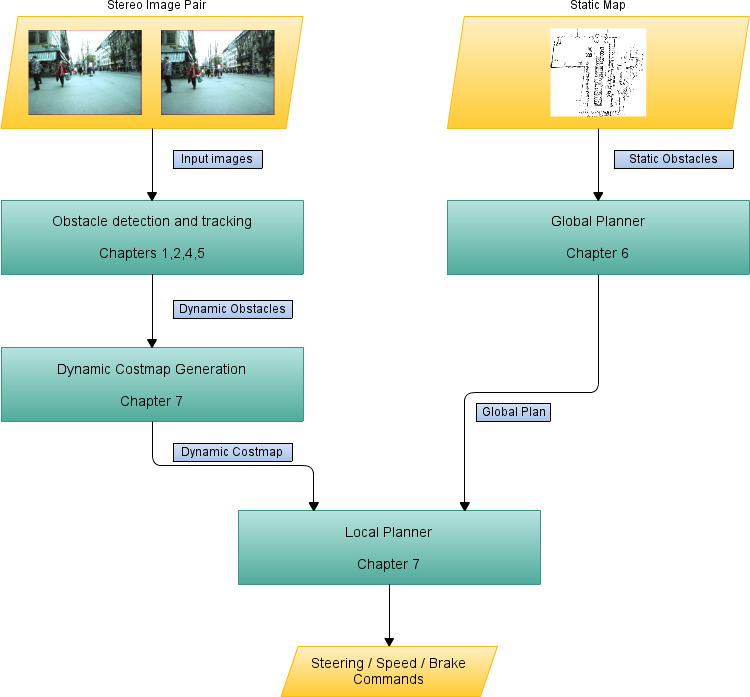
\includegraphics{pipeline_cp0}
    \end{center}
    
  \end{frame}

  
  \begin{frame}{Obstacle detection and tracking}
    \begin{itemize}
    \item<1-> Goals:
      \begin{enumerate}
      \item<2-> Good obstacle detection rate. 
      \item<3-> Obstacle localization.
      \item<4-> Real time.
      \item<5-> Environment conditions independence.
      \item<6-> Tracking capabilities.
      \item<7-> Moving cameras.
      \end{enumerate}
    \end{itemize}
  \end{frame}
  
  \begin{frame}{Obstacle detection and tracking}
    \begin{itemize}
      \item <1-> We propose four different approaches:
      \begin{enumerate}
	\item<1-> Change detection and image registration. 
	\item<2-> Background substraction and nonrigid point set registration.
	\item<3-> Stixels.
	\item<4-> Voxels and a particle filter.
      \end{enumerate}
    \end{itemize}
      
    \begin{center}
      \includegraphics<1-1>[height=.3\columnwidth]{database}
      \includegraphics<2-2>[height=.3\columnwidth]{fig6}
      \includegraphics<3-3>[height=.3\columnwidth]{stixels_over_original}
      \includegraphics<4-4>[height=.3\columnwidth]{fakePointCloud}
    \end{center}
  \end{frame}
  
  \begin{frame}{Obstacle Avoidance and Planning}
    We distinguish two different levels:
    \begin{enumerate}
     \item<1-> Global planning. 
     \item<2-> Local planning.
    \end{enumerate}

    \begin{center}
      \includegraphics<1-1>[height=.35\columnwidth]{figure7}
      \includegraphics<2-2>[height=.35\columnwidth]{example3a}
    \end{center}
  \end{frame}
  
  \begin{frame}{Evaluation of Stereo 3D Reconstruction Algorithms}
    Apart from the previous, we developed some methods intended to assess the performance of the 3D stereo reconstruction algorithms used for the particle filter based approach.
    
    \begin{center}
      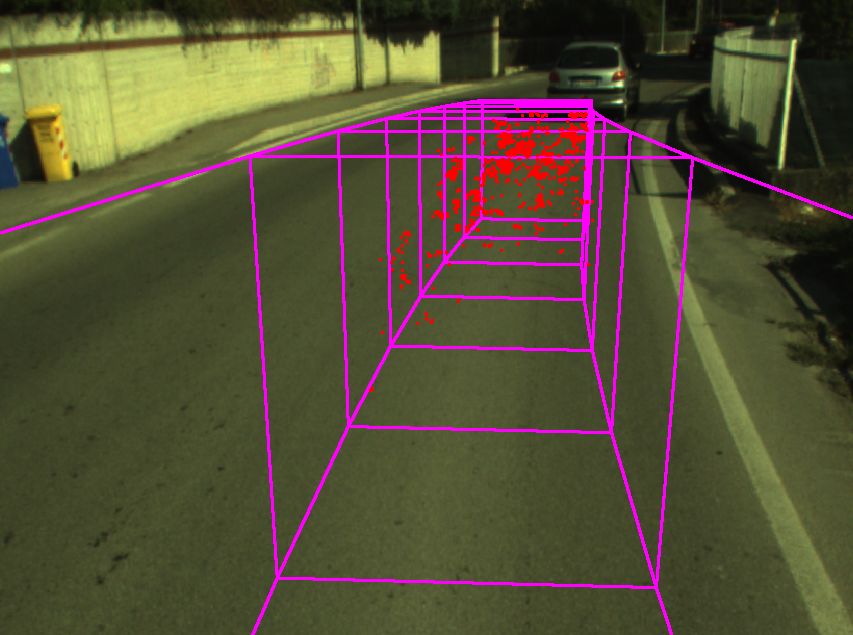
\includegraphics[height=.4\columnwidth]{fc}
    \end{center}
    
  \end{frame}
    
  \subsection{Previous Work}
  \begin{frame}{Autonomous vehicles review}
    \begin{columns}[T] % the "c" option specifies center vertical alignment
      \column{.5\textwidth} % column designated by a command
      \footnotesize
      \begin{itemize}
	\item<1-> \textbf{(1987-1995)} EC EUREKA Prometheus Project.
	\item<2-> \textbf{(1996)} ARGO Project.
	\item<3-> \textbf{(2004)} $1^{st}$ DARPA's Grand Challenge.
	\item<4-> \textbf{(2005)} $2^{nd}$ DARPA's Grand Challenge.
	\item<5-> \textbf{(2007)} DARPA's Urban Challenge.
	\item<6-> \textbf{(2010, 2012, 2013)} Korean Autonomous Vehicle Competition (AVC).
      \end{itemize}  
      \column{.5\textwidth}
      \begin{center}
	\vskip -1cm
       	\begin{overlayarea}{\textwidth}{\textheight}
	  \only<1>{
	  \begin{block}{EC EUREKA Project}
	    \begin{itemize}
	    \item VITA-2\\
	    \begin{center}\includegraphics<1->[width=0.5\textwidth]{vita2}\end{center}
	    \item VaMP\\
	    \begin{center}\includegraphics<1->[width=0.5\textwidth]{VaMP}\end{center}
	    \end{itemize}
	  \end{block}
	  }
	  \only<2>{
	  \begin{block}{ARGO Project}
	    \begin{itemize}
	      \item Lancia Thema.
	      \item Follow the lane marks of a road.
	      \item 1,900\,km
	      \item Average of 60\,Km/h.
	    \end{itemize}
	    \begin{center}\includegraphics<1->[width=0.5\textwidth]{argo}\end{center}
	  \end{block}
	  }
	  \only<3>{
	  \begin{block}{$1^{st}$ DARPA's Grand Challenge}
	    \begin{itemize}
	      \item Mojave Desert.
	      \item 240\,km route.
	      \item Listing of check points.
	      \item None finished the route.
	    \end{itemize}
	    \begin{center}\includegraphics<1->[width=0.5\textwidth]{urbanchallenge2004}\end{center}
	  \end{block}
	  }
	  \only<4>{
	  \begin{block}{$2^{nd}$ DARPA's Grand Challenge}
	    \begin{figure}[t]
		    \centering
		    \begin{subfigure}[b]{0.4\textwidth}
		      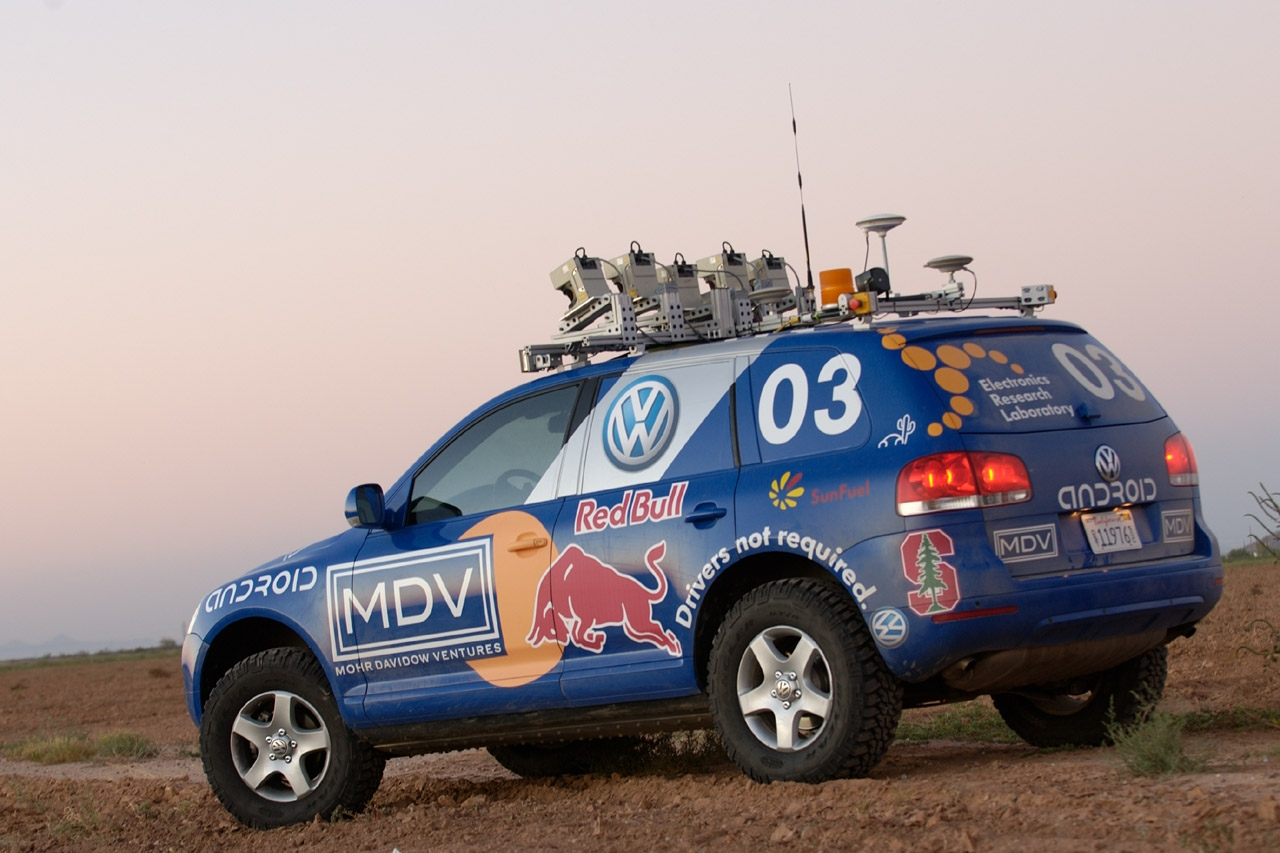
\includegraphics[width=\textwidth]{stanley}
		    \end{subfigure}
		    ~
		    \begin{subfigure}[b]{0.4\textwidth}
		      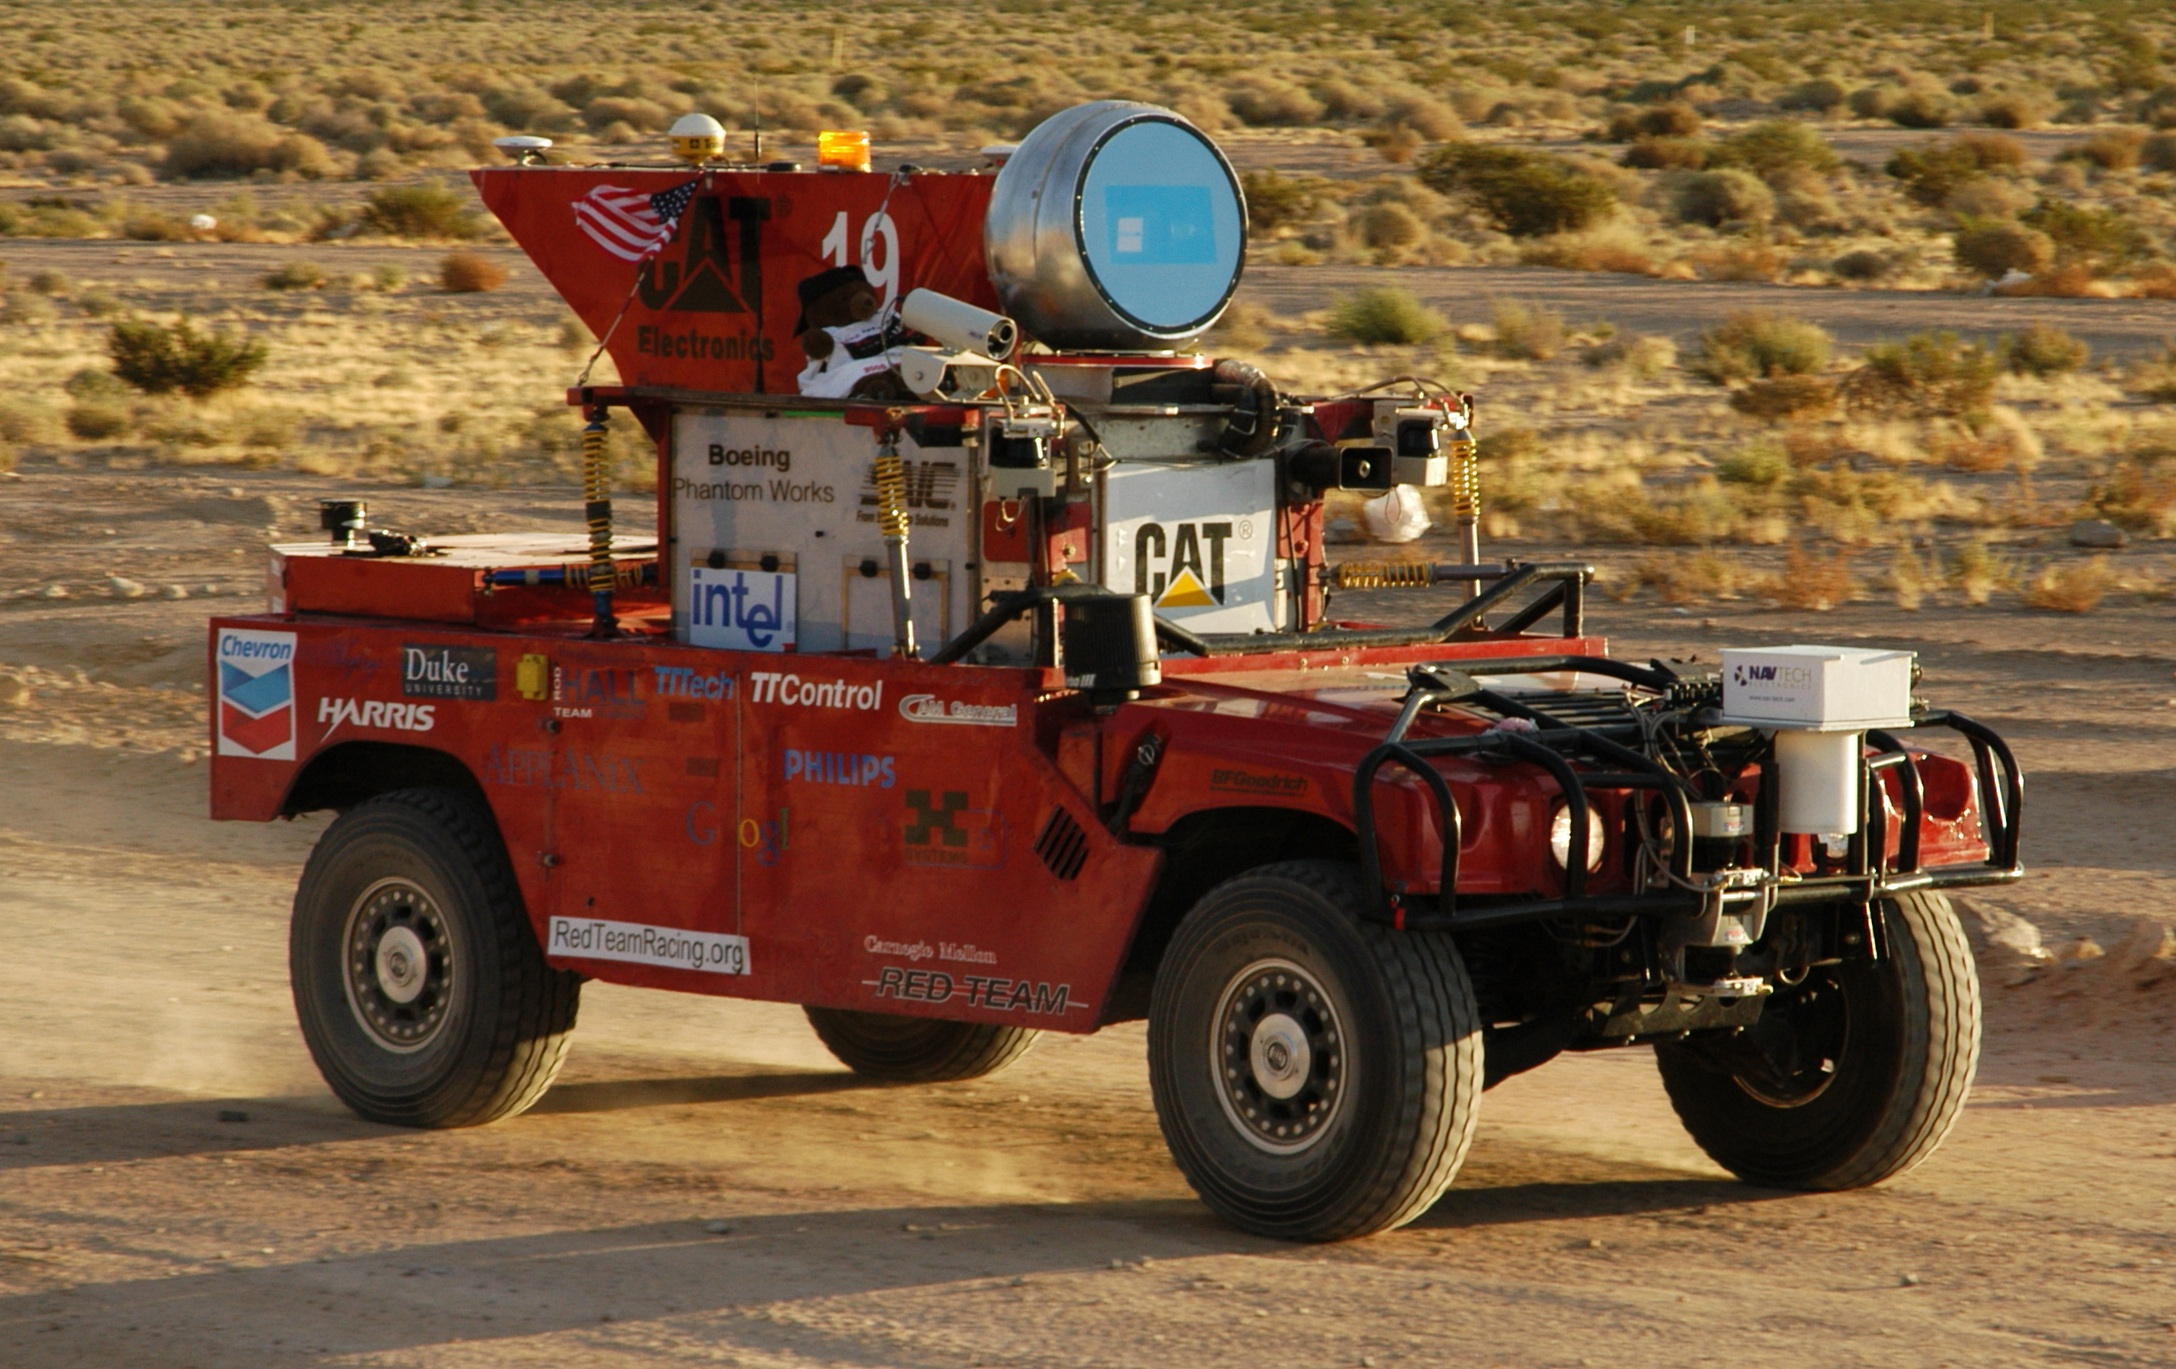
\includegraphics[width=\textwidth]{Sandstorm}
		    \end{subfigure}
		    \\~\\
		    \begin{subfigure}[b]{0.4\textwidth}
		      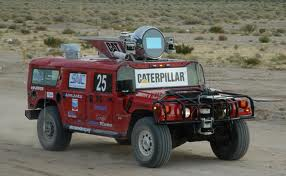
\includegraphics[width=\textwidth]{h1ghlander}
		    \end{subfigure}
		    ~
		    \begin{subfigure}[b]{0.4\textwidth}
		      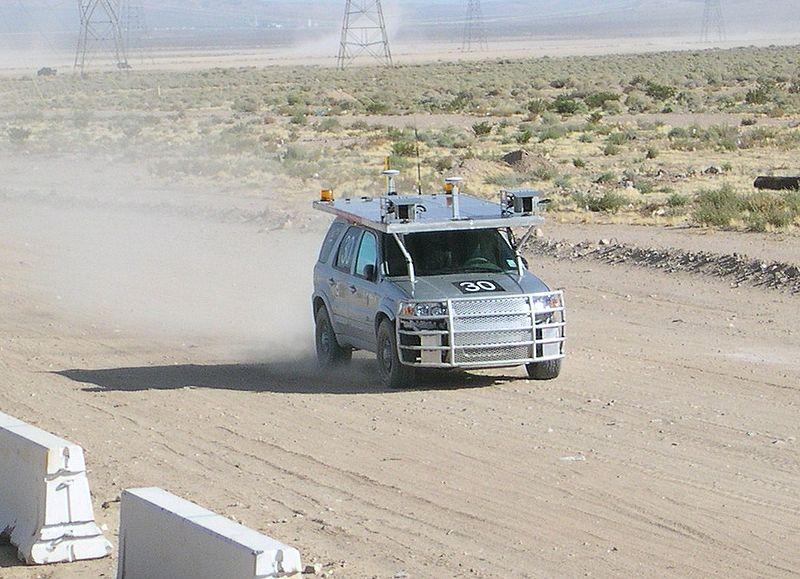
\includegraphics[width=\textwidth]{kat5}
		    \end{subfigure}
		    \\~\\
		    \begin{subfigure}[b]{0.4\textwidth}
		      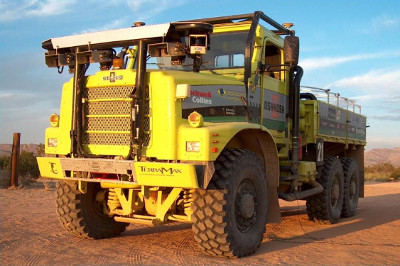
\includegraphics[width=\textwidth]{terramax}
		    \end{subfigure}
	    \end{figure}
	  \end{block}
	  }
	  \only<5>{
	  \begin{block}{DARPA's Urban Challenge}
	    \begin{figure}[t]
		    \centering
		    \begin{subfigure}[b]{0.4\textwidth}
		      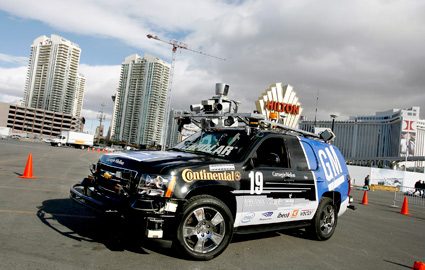
\includegraphics[width=\textwidth]{boss}
		    \end{subfigure}
		    ~
		    \begin{subfigure}[b]{0.4\textwidth}
		      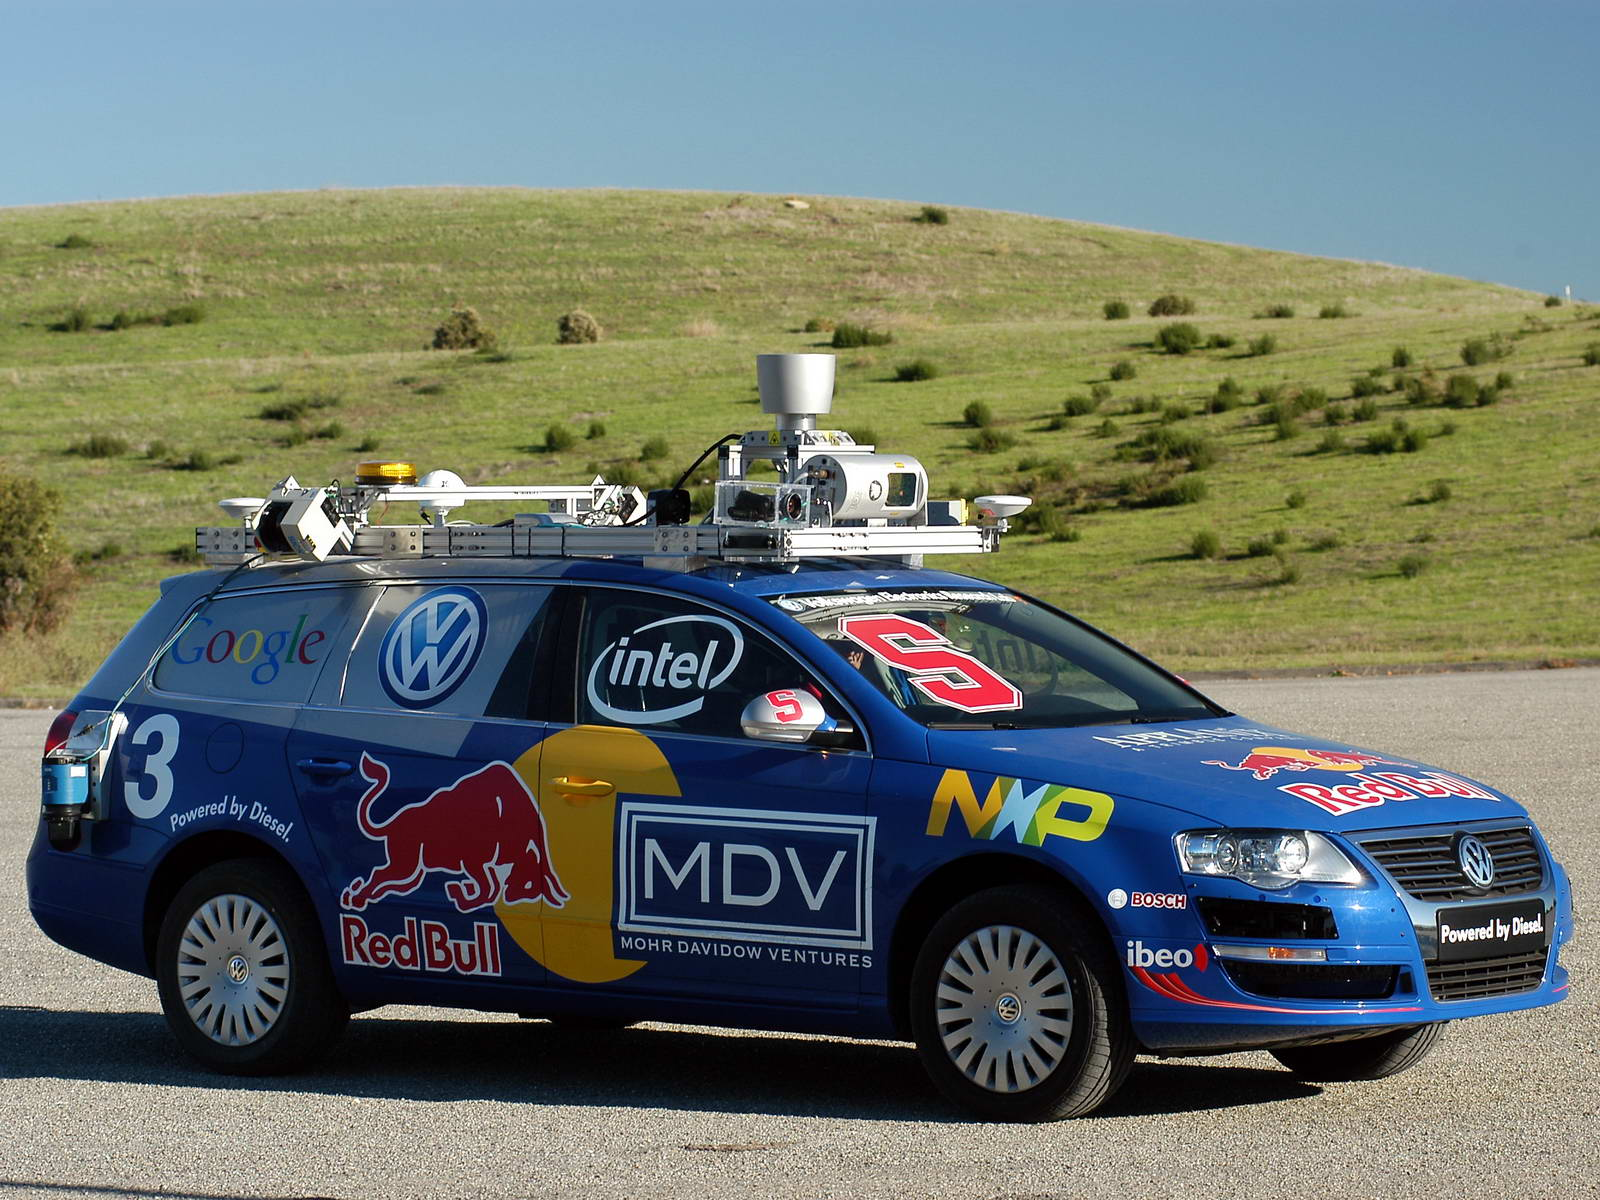
\includegraphics[width=\textwidth]{junior}
		    \end{subfigure}
		    \\~\\
		    \begin{subfigure}[b]{0.4\textwidth}
		      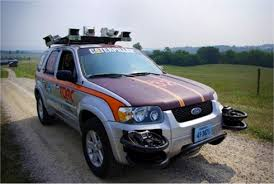
\includegraphics[width=\textwidth]{odin}
		    \end{subfigure}
		    ~
		    \begin{subfigure}[b]{0.4\textwidth}
		      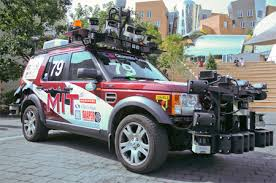
\includegraphics[width=\textwidth]{talos}
		    \end{subfigure}
		    \\~\\
		    \begin{subfigure}[b]{0.4\textwidth}
		      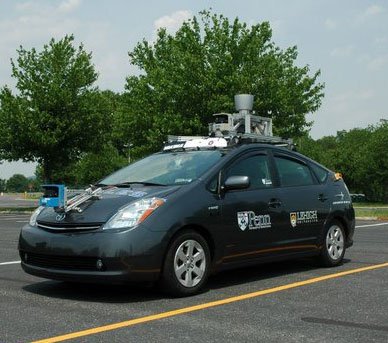
\includegraphics[width=\textwidth]{littleben}
		    \end{subfigure}
		    ~
		    \begin{subfigure}[b]{0.4\textwidth}
		      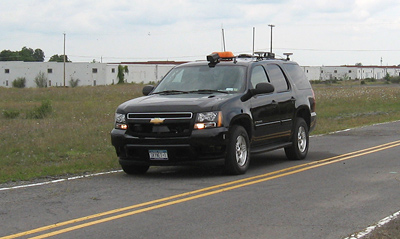
\includegraphics[width=\textwidth]{skynet}
		    \end{subfigure}

	    \end{figure}
	  \end{block}
	  }
	  \only<6>{
	  \begin{block}{Korean Autonomous Vehicle Competition (AVC)}
	    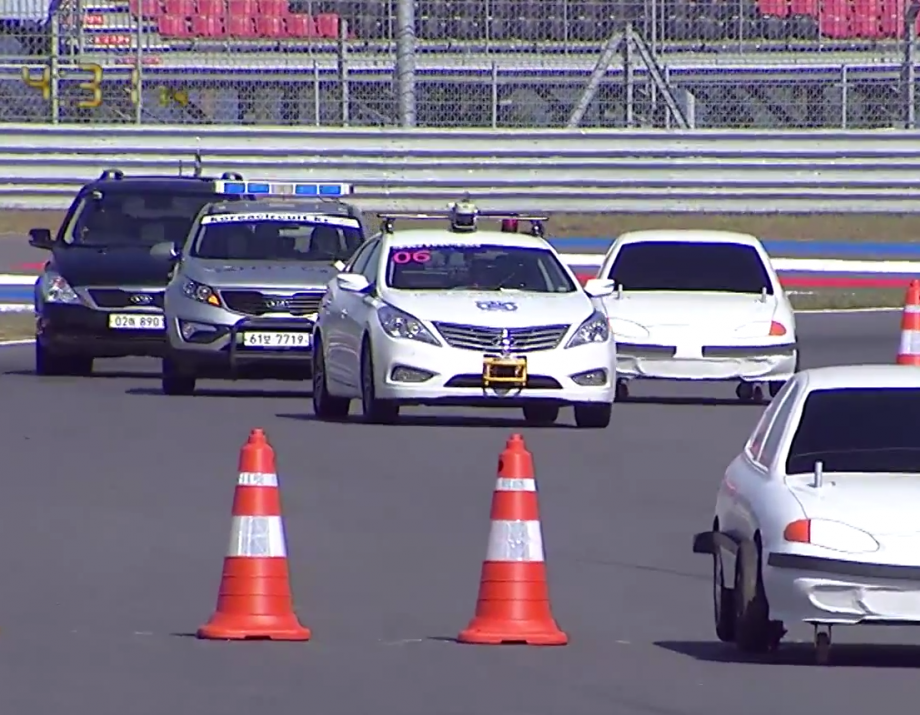
\includegraphics[width=\textwidth]{kavc}
	  \end{block}
	  }
	\end{overlayarea}
      \end{center}
    \end{columns}
    
    \note {
    \begin{itemize}
      \item From 1987 to 1995, the EC EUREKA Prometheus Project conducted research on autonomous vehicles. Among its culmination points were the twin robot vehicles VITA-2 and VaMP, driving long distances in heavy traffic.
      \item In 1996, the ARGO project modified a Lancia Thema to follow the lane marks in an unmodified highway \citep{Broggi1999}. The culmination of the project was a journey of 1,900\,km over six days on the motorways of northern Italy, with an average speed of 90 km/h. The car operated in fully automatic mode for the 94\% of its journey, with the longest automatic stretch being 55\,km. The vehicle had only two grayscale low-cost video cameras on board and used stereoscopic vision algorithms to understand its environment. 
      \item In 2004, DARPA's Grand Challenge was held in the Mojave Desert region of the United States, along a 240\,km route. This competition consisted on an autonomous vehicles race that must reach to the goal without human intervention and using just a listing of check points between the start and the finish line. None of the robot vehicles finished the route.
      \item In 2005, a second competition was held \citep{Buehler2007}. This time, five vehicles successfully completed the course:
      \begin{itemize}
      \item \emph{Stanley} \citep{thrun2006stanley}, from Standford University.
      \item \emph{Sandstorm} and \emph{H1ghlander} \citep{urmson2004high}, from the Carnegie Mellon University.
      \item \emph{Kat-5} \citep{trepagnier2006kat}, from the Gray Insurance Company.
      \item \emph{TerraMax} \citep{ozguner2004team}, from the Oshkosh Truck Corporation.
      \end{itemize}
      \item In 2007, the third driverless car competition of the DARPA Grand Challenge \citep{Buehler2009}, more known as the DARPA Urban Challenge, was held in Victorville, California. This time, six teams successfully finished the entire course:
      \begin{itemize}
      \item \emph{Boss} \citep{Urmson2008}, from the Carnegie Mellon University.
      \item \emph{Junior} \citep{montemerlo2008junior}, from Standford University.
      \item \emph{Odin} \citep{Bacha2008}, from Virginia Tech.
      \item \emph{Talos} \citep{leonard2007team}, from the Massachusetts Institute of Technology.
      \item \emph{Little Ben} \citep{bohren2008little}, from University of Pennsylvania.
      \item \emph{Skynet} \citep{miller2008team}, from Cornell University.
      \end{itemize}
      \item In 2010, 2012 and 2013, the Korean Autonomous Vehicle Competition (AVC) took place.
    \end{itemize}
    }
  \end{frame}

  \begin{frame}{Autonomous vehicles review}
    \begin{columns}[T] % the "c" option specifies center vertical alignment
      \column{.5\textwidth} % column designated by a command
      \footnotesize
      \begin{itemize}
	\item<1-> \textbf{(2010)} VIAC Challenge.
	\item<3-> \textbf{(2011)} WildCat Project.
	\item<4-> \textbf{(2011)} AutoNOMOS Group.
	\item<5-> \textbf{(2012)} Shelley.
	\item<6-> \textbf{(February 2013)} RobotCar project.
	\item<7-> \textbf{(July 2013)} BRAiVE.
	\item<8-> \textbf{(Nowadays)} Many working prototypes.
      \end{itemize}  
      \column{.5\textwidth}
      \begin{center}
	\vskip -1cm
       	\begin{overlayarea}{\textwidth}{\textheight}
	  \only<1-2>{
	  \begin{block}{VIAC Challenge}
	    \begin{itemize}
	    \item<1-> From Italy to China.
	    \item<1-> 100 day, 15,900\,km.
	    \item<2-> Four autonomous vehicles.
	    \item<2-> Limited human intervention.
	    \end{itemize}
	    \begin{center}
	      \includegraphics<1>[width=0.8\textwidth]{viacMap}
	      \includegraphics<2>[width=0.8\textwidth]{viacCars}
	    \end{center}

	  \end{block}
	  }
	  \only<3>{
	  \begin{block}{WildCat Project}
	    \begin{itemize}
	      \item Bowler Wildcat.
	      \item Oxford University.
	    \end{itemize}
	    \begin{center}\includegraphics<1->[width=\textwidth]{wildcat}\end{center}
	  \end{block}
	  }
	  \only<4>{
	  \begin{block}{AutoNOMOS Group}
	    \begin{itemize}
	      \item Spirit of Berlin.\\
	      \begin{center}\includegraphics<1->[width=0.5\textwidth]{spiritofberlin}\end{center}
	      \item MadeInGermany.\\
	      \begin{center}\includegraphics<1->[width=0.5\textwidth]{madeingermany}\end{center}
	    \end{itemize}
	  \end{block}
	  }
	  \only<5>{
	  \begin{block}{Shelley}
	    \begin{itemize}
	      \item More than 160\,km/h
	    \end{itemize}
	    \begin{center}\includegraphics<1->[width=\textwidth]{shelley}\end{center}
	  \end{block}
	  }
	  \only<6>{
	  \begin{block}{RobotCar project}
	    \begin{itemize}
	      \item Oxford University.
	      \item Switches from manual to autopilot on learned routes.
	    \end{itemize}
	    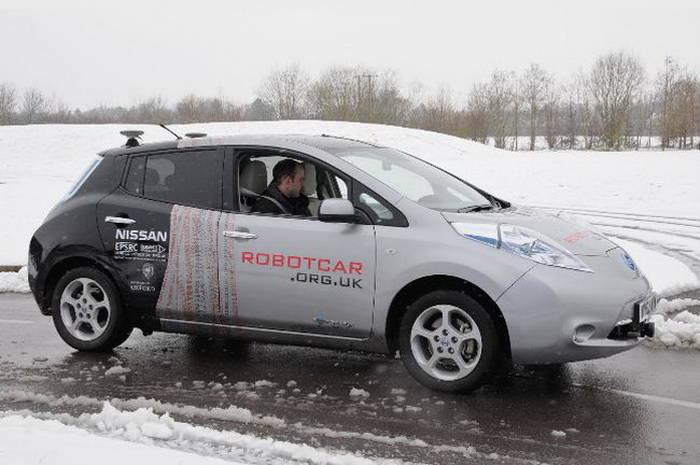
\includegraphics[width=\textwidth]{robotcar}
	  \end{block}
	  }
	  \only<7>{
	  \begin{block}{BRAiVE}
	    \begin{itemize}
	      \item Vislab.
	      \item Moved on a mixed traffic route open to public traffic.
	    \end{itemize}
	    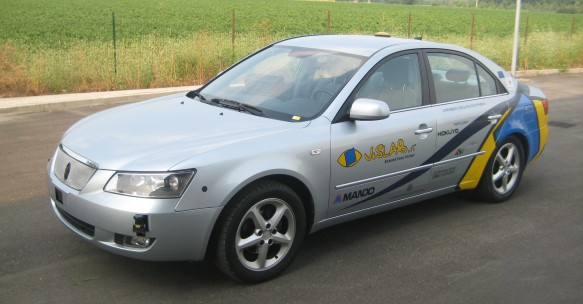
\includegraphics[width=\textwidth]{BRAiVE}
	  \end{block}
	  }
	  \only<8>{
	  \begin{block}{Many working prototypes}
	    \begin{figure}[t]
	      \centering
	      \begin{subfigure}[b]{0.2\textwidth}
		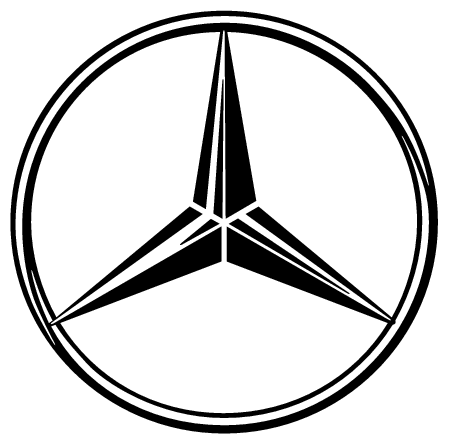
\includegraphics[width=\textwidth]{mercedes_benz}
	      \end{subfigure}
	      ~
	      \begin{subfigure}[b]{0.2\textwidth}
		
\includegraphics[width=\textwidth]{gm}
	      \end{subfigure}
	      ~
	      \begin{subfigure}[b]{0.2\textwidth}
		
\includegraphics[width=\textwidth]{continental}
	      \end{subfigure}
	      \\~\\
	      \begin{subfigure}[b]{0.2\textwidth}
		
\includegraphics[width=\textwidth]{autoliv}
	      \end{subfigure}
	      ~
	      \begin{subfigure}[b]{0.2\textwidth}
		
\includegraphics[width=\textwidth]{bosch}
	      \end{subfigure}
	      ~
	      \begin{subfigure}[b]{0.2\textwidth}
		
\includegraphics[width=\textwidth]{nissan}
	      \end{subfigure}
	      \\~\\
	      \begin{subfigure}[b]{0.2\textwidth}
		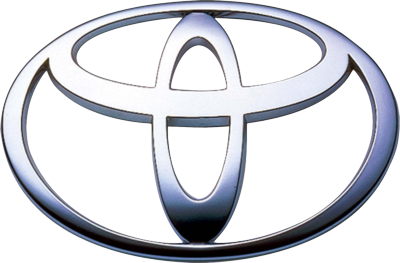
\includegraphics[width=\textwidth]{toyota}
	      \end{subfigure}
	      ~
	      \begin{subfigure}[b]{0.2\textwidth}
		
\includegraphics[width=\textwidth]{audi}
	      \end{subfigure}
	      ~
	      \begin{subfigure}[b]{0.2\textwidth}
		
\includegraphics[width=\textwidth]{vislab_logo}
	      \end{subfigure}
	      \\~\\
	      \begin{subfigure}[b]{0.2\textwidth}
		
\includegraphics[width=\textwidth]{oxforduni_logo}
	      \end{subfigure}
	      ~
	      \begin{subfigure}[b]{0.2\textwidth}
		
\includegraphics[width=\textwidth]{google}
	      \end{subfigure}
	    \end{figure}
	  \end{block}
	  }
	\end{overlayarea}
      \end{center}
    \end{columns}
    
    \note {
    \begin{itemize}
      \item In 2010, inside the VIAC Challenge, four autonomous vehicles drove from Italy to China on a 100-day 15,900\,km trip with only limited human intervention (in traffic jams and when passing toll stations). At the time, this was the longest-ever journey conducted by an unmanned vehicle \citep{Broggi2010VIAC}.
      \item In 2011, under the Oxford University's WildCat Project, a Bowler Wildcat based prototype is capable of autonomous operation using a flexible and diverse sensor suite.
      \item In 2011, the Freie Universität Berlin, Led by the AutoNOMOS group, developed two autonomous cars - \emph{Spirit of Berlin} \citep{berlin2007spirit} and \emph{MadeInGermany} \citep{gohring2013semi} - to drive in the innercity traffic of Berlin in Germany. They were able to handle intercity traffic, traffic lights and roundabouts between the International Congress Centrum and the Brandenburg Gate.
      \item In 2012, Stanford's Dynamic Design Lab, in collaboration with the Volkswagen Electronics Research Lab, produced Shelley, an Audi TTS designed for high speed (greater than 160\,km/h) on a racetrack course.
      \item In February 2013, Oxford University unveiled the RobotCar UK project, an inexpensive autonomous car capable of quickly switching from manual driving to autopilot on learned routes.
      \item In July 2013, Vislab worldpremiered BRAiVE, a vehicle that moved autonomously on a mixed traffic route open to public traffic \citep{grisleri2010braive}.
      \item Currently, many major companies and research organizations have developed working prototype autonomous vehicles, including Mercedes-Benz, General Motors, Continental Automotive Systems, Autoliv Inc., Bosch, Nissan, Toyota, Audi, Vislab (University of Parma), Oxford University and Google.
    \end{itemize}
    }
  \end{frame}
  
  \begin{frame}{Obstacle detection}
    We can divide object tracking methods into two subcategories:
    \begin{itemize}
      \item \emph{2.5D Solutions:} Different approaches:
      \begin{itemize}
	\item \emph{Use of the 3D point as feature.} \cite{franke20056d}
	\item \emph{Dynamic stixels.} \cite{badino2009stixel, pfeiffer2011towards, pfeiffer2013exploiting, benenson2011stixels, benenson2012pedestrian, benenson2012fast}
	\item \emph{Tracked image features.} \cite{barth2009estimating}
	\item \emph{Sensor fusion.} \cite{wu2009collision}
	\item \emph{Occupancy grids.} \cite{danescu2012particle}
      \end{itemize} 
      \item \emph{3D Solutions}
      \begin{itemize}
	\item \emph{Octree connected cubes.} \cite{broggi2013}
	\item \emph{Adjacent stacks of cells} \cite{Moravec96robotspatial}
      \end{itemize}
    \end{itemize}
    
    \note{
    Based on how much information they use, we can divide object tracking methods into two subcategories:
    \begin{itemize}
      \item \emph{2.5D Solutions:} They do not make use of the complete information provided by 3D points. Instead of that, they tend to use elevation maps composed of uniform size cells. Each cell just stores occupancy and height information. This is the kind of methods that, as described before, usually consider obstacles as being in contact with a flat ground.
      In these methods, tracking is performed before the complete reconstruction is done, in an intermediate point based on an specific feature. Depending on the feature used, we distinguishing different approaches:
      \begin{itemize}
	\item \emph{Use of the 3D point as feature.} An example of this is the so called 6D vision \citep{franke20056d}, in which the 3D stereo vision extracted information is combined with an efficient implementation of an optical flow in the image space based on a \ac{GPU}. Relevant points are tracked using a Kalman filter.
	\item \emph{Dynamic stixels.} This approach has been longer discussed in section \ref{ch:chapter00_02_04}.
	\item \emph{Tracked image features.} An example is the work by \cite{barth2009estimating}. There, obstacles are represented as a rigid 3D point set which are tracked in terms of feature displacements and depth measurements.
	\item \emph{Sensor fusion.} \cite{wu2009collision} reconstruct the objects as cuboids from a stereo point cloud. In this process, position and speed values are improved to a very accurate value by the use of a radar along with stereo.
	\item \emph{Occupancy grids.} This is a very popular choice for tracking. An occupancy grid is a probabilistic map of the driving environment, which encodes the past and present knowledge from sensor data, and which can be updated dynamically when new information is available. These occupancy grids can be cartesian, with rectangular cells, polar, or even a relation between columns in an image and the disparity. An example of this is the method by \cite{danescu2012particle}, which has inspired part of the work described in chapter \ref{ch:chapter05}.
	Another advantage of the model based on an occupancy grid is that it makes easier a collaborative update of the grid, which allows the usage of data from several sensors and observers. Another simple example of occupancy grid is that described in chapter \ref{ch:chapter07}.
      \end{itemize} 
      \item \emph{3D Solutions:} Usually based on complex grid maps that use complete 3D information. Again, depending on how this grid is represented, we find 
      \begin{itemize}
	\item \emph{Octree connected cubes.} An example is the work by \cite{wurm2010octomap} or \cite{broggi2013}.
	\item \emph{Adjacent stacks of cells}, as described in \cite{Moravec96robotspatial} 
      \end{itemize}
    \end{itemize}
    }
  \end{frame}

  \begin{frame}{Path planning}
    \begin{itemize}
      \item Classical methods \citep{hwang1992gross}
      \item Heuristic methods \citep{masehian2007classic}
      \item SVM based methods
      \begin{itemize}
       \item Global
	 \begin{itemize}
	  \item \cite{miura2006support}
	  \item \cite{yang2012safe}
	 \end{itemize}
       \item Local
	\begin{itemize}
	  \item \cite{sarkar2008mobile}
	  \item \cite{tennety2009support}
	  \item \cite{qingyang2012local}
	\end{itemize}
      \end{itemize}
    \end{itemize}
    
    \note{
      About classical methods, in general they can be considered as variations of some general approaches: Roadmap, Cell Decomposition, Potential Fields and Mathematical Programming. These methods are not mutually exclusive; in fact, a lot of approaches use combinations of them. A review of some classical methods can be checked out in \cite{hwang1992gross}.
 
      About heuristic methods, these are the answer given by researchers to the limitations of the classic methods. The most representative methods inside this classification are Probabilistic Roadmaps (PRM) \citep{kavraki1996probabilistic}, Rapidly Exploring Random Trees (RRT) \citep{lavalle2000rapidly}, Level set \citep{sethian1999level}, Linguistic Geometry (LG) \citep{stilman1993network}, Simulated Annealing (SA) \citep{zhu2006robot}, Artificial Neural Network (ANN) \citep{hossain2012real}, Genetic Algorithms (GA) \citep{zhang2007evolutionary}, Particle Swarm Optimization (PSO) \citep{chen2006smooth}, Ant Colony (ACO) \citep{mou2008modified} and its variants, like the RNA algorithm described in \cite{zhu2011new}, Stigmergy \citep{cazangi2006evolutionary}, Wavelet Theory \citep{doh2005systematic}, Fuzzy Logic (FL) \citep{kladis2011energy} and Tabu Search (TS) \citep{nguyen2012multi}. For more information, the review in \cite{masehian2007classic} can be checked.
      
      Global:
      In the work presented by \cite{miura2006support}, navigation is planned in environments in which the obstacles are known. Obstacles are randomly labeled into two classes: positive or negative. Using these two classes, a \ac{SVM} is trained and the decision boundary is used as a path. To increase the efficiency, a set of fake obstacles (guide samples) is generated at both sides of the current and goal position, as well as in parallel to the line that joins both points (nominal line), with the objective of helping the \ac{SVM} to find a feasible path.
      \cite{yang2012safe}. In their work, a preprocessing step is used in which the Voronoi Diagram is generated using the obstacles in the map. That diagram is used to select the best path between the starting point of the robot and the goal. The path obtained using Voronoi is not smooth, so the \ac{SVM} is used to make this path smoother. The \ac{SVM} is trained using a dataset in which the sites that generated the Voronoi edges are classified as positive or negative depending on their position (left / right) regarding to the previously obtained path. The decision boundary of this \ac{SVM} will be the final path used.
      
      Local:
      In \cite{sarkar2008mobile, tennety2009support}, authors divide the whole set of objects in the map into two classes and the \ac{SVM} is used to determine the maximum margin hyperplane between the data sets belonging to the two classes. Data is assigned to one or another class depending on whether the points are on the left or on the right side of the robot. Once the initial labels are assigned, further classification is done using the k-nearest neighbor algorithm, with k=1.
      \cite{qingyang2012local}, that uses a path subdivision method and a \ac{SVM}. They use topological maps of local environments which are extracted with little expanded nodes. Next, candidate routes are optimized using the Support Vector Machine, where the candidate routes boundary points are defined as positive and negative samples. They also extend the original \ac{SVM} \citep{cortes1995support} in order to satisfy extra constraints such as vehicle position and heading.
    }
  \end{frame}
  
    \begin{frame}{Local planning}
    \begin{itemize}
      \item \cite{werling2010optimal}
      \item \cite{thrun2006stanley}
      \item \cite{chu2012local}
    \end{itemize}
     
    \note{
      \begin{itemize}
	\item In \cite{werling2010optimal}, long term objectives are performed, like speed keeping, merging, following, stopping. This is done through optimal control strategies within the Fren\'et frame of the street.
	\item In \cite{thrun2006stanley}, lateral offset is defined as the perpendicular to an established base trajectory. This allows the vehicle driving along the road parallel to this trajectory. In order to select the optimal path, the cost function penalizes passing over obstacles and the distance respect to the center of the current road.
	\item In \cite{chu2012local}, also a set of candidate paths are generated, with endpoints in fixed positions at different offsets respect to the base frame, but they do not set this base frame in the center of the road, since it could be dangerous when computing the costs at certain scenarios. Instead of that, they use a security cost for each candidate path. Security of the path is computed by blurring the binary data of the obstacles. They also have into account certain criteria, as the smoothness cost or the path consistency between iterations.
      \end{itemize}
    }
  \end{frame}
  
  \subsection{Testing platform}
  \begin{frame}{Testing platform}
    These algorithms are intended to be used in Verdino.
    \begin{itemize}
     \item<1-> Prototype developed by GRULL, Universidad de La Laguna.
     \item<2-> It will transport people around a bioclimatic urbanization in the ITER facilities.
     \item<3-> A golf cart has been modified to be used as an unmanned vehicle.
    \end{itemize}

    \begin{center}
      \includegraphics<1-1>[height=.3\columnwidth]{verdino}
      \includegraphics<2-2>[height=.3\columnwidth]{iter}
      \includegraphics<3-4>[height=.3\columnwidth]{NV_TXT2}
      \includegraphics<4-4>[height=.3\columnwidth]{verdino}
    \end{center}
  \end{frame}
  
  \begin{frame}{Actuators}
    \begin{columns}[c] % the "c" option specifies center vertical alignment
      \column{.5\textwidth} % column designated by a command
      \begin{itemize}
	\item<1-> Steering system.      
	\item<2-> Braking system.
	\item<3-> Speed system.
	\item<4-> Safety switch.
      \end{itemize}  
      \column{.5\textwidth}
      \begin{center}
	\includegraphics<1-1>[width=\textwidth]{steering}
	\includegraphics<2-2>[width=\textwidth]{braking}
	\includegraphics<3-3>[width=\textwidth]{speedControl}
	\includegraphics<4-4>[width=\textwidth]{panicbutton}
      \end{center}
    \end{columns}
    
    \note {
    \begin{itemize}
      \item Steering system: we tied the original steering to a DC motor controlled by a PID.
      \item Braking system: Controlled through a pneumatic system, composed by a cylinder, a commutation valve, two flow controllers and an air compressor. The pneumatic cylinder acts over the brake cables, that make pressure over the brake drums. A compressor gives the air pressure needed for this process.
      \item Speed system: A microcontroller generates three different signals, that simulate the original devices installed in the vehicle. These correspond to a switch relay, which turns on the motor when the user pushes the acceleration pedal; the sense of speed (forward or backward); and the desired voltage
      \item Safety switch: Allows changing between automatic and manual behavior. When switched off, the vehicle behaves as it was before the modifications.
    \end{itemize}
    }
  \end{frame}

  \begin{frame}{Sensors}
    \begin{columns}[c] % the "c" option specifies center vertical alignment
      \column{.5\textwidth} % column designated by a command
      \begin{itemize}
	\item<1-> Localization sensors.      
	\begin{itemize}
	  \item<3-> Odometry.      
	  \item<4-> IMU.
	  \item<5-> Differential GPS.
	\end{itemize}  
	\item<2-> Navigation sensors.	
	\begin{itemize}
	  \item<6-> LIDAR.      
	  \item<7-> IR cameras.
	  \item<8-> Visible cameras.
	\end{itemize}
      \end{itemize}  
      \column{.5\textwidth}
      \begin{center}
	\includegraphics<3-3>[width=\textwidth]{odometry}
	\includegraphics<4-4>[width=\textwidth]{imu}
	\includegraphics<5-5>[width=\textwidth]{dgps}
	\includegraphics<6-6>[width=\textwidth]{lidar}
	\includegraphics<7-7>[width=\textwidth]{ircameras}
	\includegraphics<8-8>[width=\textwidth]{visiblecamera}
      \end{center}
    \end{columns}
    
    \note {
    \begin{itemize}
      \item \emph{Odometry}: This system measures the independent movement of the two rear wheels, which are attached to an optical encoder. This allows computing the position, orientation and speed of the prototype incrementally.
      \item \emph{\acf{IMU}}: It is comprised by 9 sensors (3 accelerometers, 3 gyroscopes and 3 magnetometers), which are fused in real time in order to get the three-dimensional orientation of the vehicle. The model of the sensor is a \emph{Xsens Mti}.
      \item \emph{\acf{DGPS}}: Allows positioning the vehicle with centimetric accuracy. It is composed by two different devices, the reference station, which is fixed in a known place, and the rover station, which is installed on the vehicle. The model used is a \emph{JAVAD GNSS Triumph-1}, which has an horizontal precision below 1\,cm and a vertical precision around 1.5\,cm using \ac{DGPS}, at a frequency of $5\,Hz$.
      \item \emph{\acf{LIDAR}}: These are used also for localization purposes. Each of those sensors is able to detect the objects in the way of the vehicle, at the plane in which the sensor is mounted. The advantages of these sensors are that they have a high speed and precision. However, they are just able to detect obstacles that crosses the plane defined by the sensor. Because of this, we have equipped the vehicle with 5 \acp{LIDAR}. Two of them are located at the same plane in the front corners of the vehicle, at a height of 50\,cm. Each of these covers an angle of 270\textdegree. Another is located in the front side of the vehicle, at a height of 20\,cm, slightly tilted upwards, in order to detect the small obstacles or non traversable areas. Another is in the top of the vehicle, also in the front side of the vehicle, tilted to the ground and covering the blind areas left by the other sensors. Finally, the last sensor is situated in the back side of the vehicle, and it is used for backwards maneuvers. The used sensors are of the model \emph{SICK LMS 100} and \emph{SICK LMS 111}, allowing a maximal detection distance of 20\,m, a precision of 10-35\,mm, a maximal angular resolution of 0.25\textdegree and a maximal rate of $50\,Hz$.
      \item \emph{IR cameras}: Infrared cameras are used to detect pedestrians or animals based on their temperature. We have a pair of them installed on a Pan-Tilt system attached to the top front side of the vehicle. The model used is a \emph{MobiR\textregistered~M3}, which is able to detect objects in the range $8\sim14\mu m$, at a resolution of $160 \times 120\,px$.
      \item \emph{Visible cameras}: A set of three cameras is also installed in a pan-tilt structure. These are used for the detection and tracking of the objects, which is one of the goals of this thesis. Also, they are currently being used for the detection of the borders of the road. The model of the cameras is a \emph{GoPro\textregistered Hero 3 silver edition}, with a $1920 \times 1080 \, px$ maximal video resolution and a 170\textdegree field of view at a maximal rate of 60\,fps.
    \end{itemize}
    }
  \end{frame}
  
  \begin{frame}{Control}
    \begin{columns}[c] % the "c" option specifies center vertical alignment
      \column{.5\textwidth} % column designated by a command
      \begin{itemize}
	\item<1-> Onboard computer.   
	\begin{itemize}
	  \item<2-> i7-3770K.      
	  \item<2-> 16 Gb RAM DDR3.
	  \item<2-> SSD Storage.
	\end{itemize}	
	\item<3-> Low-level control.
      \end{itemize}  
      \column{.5\textwidth}
      \begin{center}
	\includegraphics<1->[width=\textwidth]{onboard}
      \end{center}
    \end{columns}
    
    \note {
    The vehicle is controlled, at high level, by an on board computer equipped with an \emph{i7-3770K} processor, 16\,Gb of \emph{RAM DDR-3} memory and a \emph{SSD} storage. At low level, a set of own developed electronic devices receive commands from the computer and transform them into the right signal, understandable by the actuators described before.
    }
  \end{frame}
  

% \mainmatter
% \part{Obstacle detection}
% %%
%%  chapter01.tex - Obstacle Detection and Planning for Autonomous Vehicles based on Computer Vision Techniques
%%
%%  Copyright 2014 Néstor Morales <nestor@isaatc.ull.es>
%%
%%  This work is licensed under a Creative Commons Attribution 4.0 International License.
%%

\graphicspath{{./images/chapter01/bmps/}{./images/chapter01/vects/}{./images/chapter01/}}

\chapter{Problem Statement and Previous Work}\label{ch:chapter01}

\section{Problem Statement}\label{ch:chapter01_01}

Computer Vision environment understanding targeted at enabling autonomous operation of a robotic platform has been widely studied over the years, leading to the creation of some prototype vehicles \cite{Maurer1996,Pomerleau1996,Broggi1999} which demonstrated that negotiating moderately complex and dynamic situations in real time was possible, albeit challenging. However, it was only with the development effort driven by the DARPA Challenges \cite{Buehler2007, Buehler2009} that the technology required to provide reliable operation both in off-road and urban scenarios proved to be within reach.
The vehicles that successfully took part to this series of events had to integrate planning and actuation capabilities with a sensing suite capable of coping with harsh environments, heavy traffic and wide temperature ranges, while keeping functional over extended amounts of time. Most competitors relied on high-end active sensors \cite{Urmson2008, Montemerlo2008, Bacha2008, Kammel2008}, with some notable exceptions \cite{Broggi2006, Broggi2010}. 

As we discover when looking up to the available literature (See next section, \ref{ch:chapter01_02}), there are many methods for the detection and tracking of obstacles in complex environments, like this for which Verdino is intended to be working. In this sense, a very first approach is that inspired on the work by \cite{primdahl2005change},  \cite{diego2011video} or \cite{vallespi2012prior} was developed. This is based on the fact that, in an image, a high percentage of the scene represented usually corresponds to static objects. Based on that, it looks quite straightforward to think that, having an image representing an area without obstacles, it is possible to detect the obstacles in an scene by just comparing it with an image being taken in real time. For that, we obtained a dataset with geo-referenced images from a closed urbanization taken at different times of the day. A description of this database, as well as of the algorithm pipeline used for the comparison between images pairs can be found at section \todo{ \ref{XXX} }.

However, such approach suffers from several drawbacks. First, as we just use one image per frame, we are no able to know the exact position of the obstacle in the real world \comment{(Anyway, we think that the output of the algorithm is a good starting point for a classification method)}. Also, the quality of detection is highly tied to the size of the image database, so in big areas we need a huge dataset, with the related space and throughput problems associated to that. If we consider changes due to weather or light conditions, this dataset grows exponentially. Finally, we don't know the direction where an obstacle is going to. These are challenging problems that have been solved using different approaches, until we reached a final solution, described in section \todo { \ref{XXX} }.

To solve that, we first developed a method that tries to isolate just the tracking problem with the use of static monocular cameras. Instead of registering pairs of images, we segment the image with the use of foreground extraction techniques, distinguishing between background and foreground. Using the silhouette of the objects in the foreground (which are mainly non-rigid objects, like pedestrians or animals), we apply a non-rigid point set registration algorithm in order to track the different parts of the body of the obstacles separately. This method, inspired in works like those by \cite{starck2007surface}, or \cite{letouzey2011scene}, can be also used for the completion of the global map of the vehicle, or even for tasks more related to \acf{HMI}. This approach is extensively described in section \todo{ \ref{XXX}}.

However, this method still makes use of a very rudimentary method for the localization of the obstacles (See section \todo{ \ref{XXX-subsection_localization}}), and it is limited to static cameras. For the application proposed, we need the cameras installed on the top of the moving prototype, so we can not use foreground segmentation methods anymore for the detection of the objects in the road. A simple solution for that is stop using monocular vision, and start using stereo vision. In the last years, a high number of advanced algorithms has become viable for autonomous driving applications. The problem is that performing a quantitative and meaningful comparison of their performance level, however, is not an easy task, mainly because of the difficulty of producing ground truth information. Older datasets are small, and either synthetic or taken in controlled environments (\cite{Scharstein2002}), thus effectively limiting their usefulness as indicators of the actual algorithms ability to cope with outdoor scenarios. Due to that, it is needed to compare the performance level of some state-of-the-art stereovision-based 3D mapping algorithms in automotive scenarios. This evaluation methodology and the associated results is shown in section \todo{ \ref{XXX}}. \comment{PREGUNTAR A LA GENTE DEL VISLAB SI ESTA DE ACUERDO CON QUE USE ESTO EN LA TESIS, POR SI LAS MOSCAS}.

\comment{Este párrafo y la sección asociada dependerá de lo que consiga sacar más adelante.}\notsure{
Apart from the full-dense 3D reconstruction methods, we also explore the possibility of using a simpler (and faster) reconstruction based on Stixels, like that described by \cite{badino2009stixel}. In particular, we decided to use the implementation by \cite{benenson2012pedestrian}, due to its fast response (about 100 frames per second). The method, described in section \todo{\ref{XXX}}, compares the stixels obtained between frames and tracks the obstacles along the time. This solves all the problems we had: we can use moving cameras, we can locate the obstacles in the map, and also we are able to know the path followed by them.}

Another approach, which makes use of the dense stereo reconstruction algorithms for which we did the evaluation described above, is inspired in the work by \cite{danescu2012particle}, but also from the voxelized world described in \cite{broggi2013}. The key idea is to simplify the 3d reconstructed world into a grid of voxels, each of these representing a certain volume in the world. In this voxelized world, for each voxel above a given occupancy probability threshold, a set of particles part of a particle filter is assigned. Each particle will have a double function: the first, denoting hypotheses (as in the classical particle filter methods); the second, to be used as segmentation criteria in the segmentation of the world into different obstacles. In this way, we consider that two contiguous voxels belong to different obstacles if their obtained direction and sense diverges. A more detailed explanation of the method is found in \todo{\ref{XXX}}.

At this point, we have an acceptable reconstruction of the surroundings of the vehicle, which includes the localization and tracking of the obstacles in the neighborhood of the cart. But the reconstruction of the environment is not the only challenge that an autonomous vehicle has to deal with. Once that a vehicle has an idea of where it is, and where it wants to go, it also needs to know the best way to reach there and, more important, how to avoid the harmful elements it has previously detected using the methods described. This allows a safe trip, both for the pedestrians, cars, etc. in the road, and for the vehicle itself.
As said, Verdino is intended to travel in pedestrian areas where most of the obstacles are pedestrians, so its behavior must be mainly reactive in order to give priority to the safety of paths against the efficiency of the route. Also, there is not a clear traveling path, like a road. Instead of that, the vehicle will be moving around an unstructured area, so there is not something like a \acf{RNDF} that allows a fast calculation of the paths that the car will use to reach a certain point. Because of that, we must consider two different planning levels:
\begin{itemize}
 \item \textbf{Global Planning:}
 As it is not possible to determine a global trajectory based on a \acs{RNDF}, we must use a method able to deal with changing environments for the calculation of a fast and safe path. The idea is that, having a map of the static obstacles in the environment and with the vehicle properly localized on it \cite{Perea2013mcl}, it will generate a path that will allow reaching this destination as fast as possible. This task, which can be solved easily in static environments using graphs or other similar optimization methods, becomes a little bit more challenging in environments like, for example, a parking lot, in which cars are parking and driving off continuously.
 In section \todo{ \ref{XXX} }, the way in which we solved this problem is described. It is based on the border between classes, which is obtained after training a \acf{MSVM} (See Appendix \todo {\ref{XXX}} for more information), considering each single obstacle as a separate class. Instead of using this border for classification purposes, as it is usual, we take advantage of the fact that it will be the safest and smoother distance to the obstacles. Taking this into account, it makes sense to apply this separation line as our path. Also, the use of a different class for each obstacle allows ensuring that the path is safe enough, even in complicate scenarios, like in pedestrian areas.
 
 \item \textbf{Local Planning:}
 In a lower level, we also need a way to make the vehicle know how to follow the generated path. This problem requires a system able to, several times per second, calculate the best steering angle and speed in order to follow the global plan while avoiding the surrounding obstacles. The method, which is inspired in the work of \cite{chu2012local}, receives as input the current position of the vehicle in the map, its orientation, speed and the steering angle. Also, we provide it with the global plan obtained in the upper level. Finally, a map of the dynamic obstacles in the surrounds of the cart is computed and passed to the algorithm.
 
 This dynamic map can be filled with the information provided by sensors like \acp{LIDAR}, among other sensors. But it can can also be computed with the information extracted from cameras, and this is the connection point with the work described in the first part of this Thesis. The detected obstacles are included in the map, so the vehicle is able to avoid them using the calculated steering angle and speed.
 
 The way in which both this map and the speed/steering angle commands is obtained is described in section \ref{XXX}.
\end{itemize}
 
 The whole pipeline of the application developed for this thesis is shown at figure \ref{fig:cp01_pipeline}. 
 
\begin{figure}[thb]\label{fig:cp01_pipeline}
  \centering
  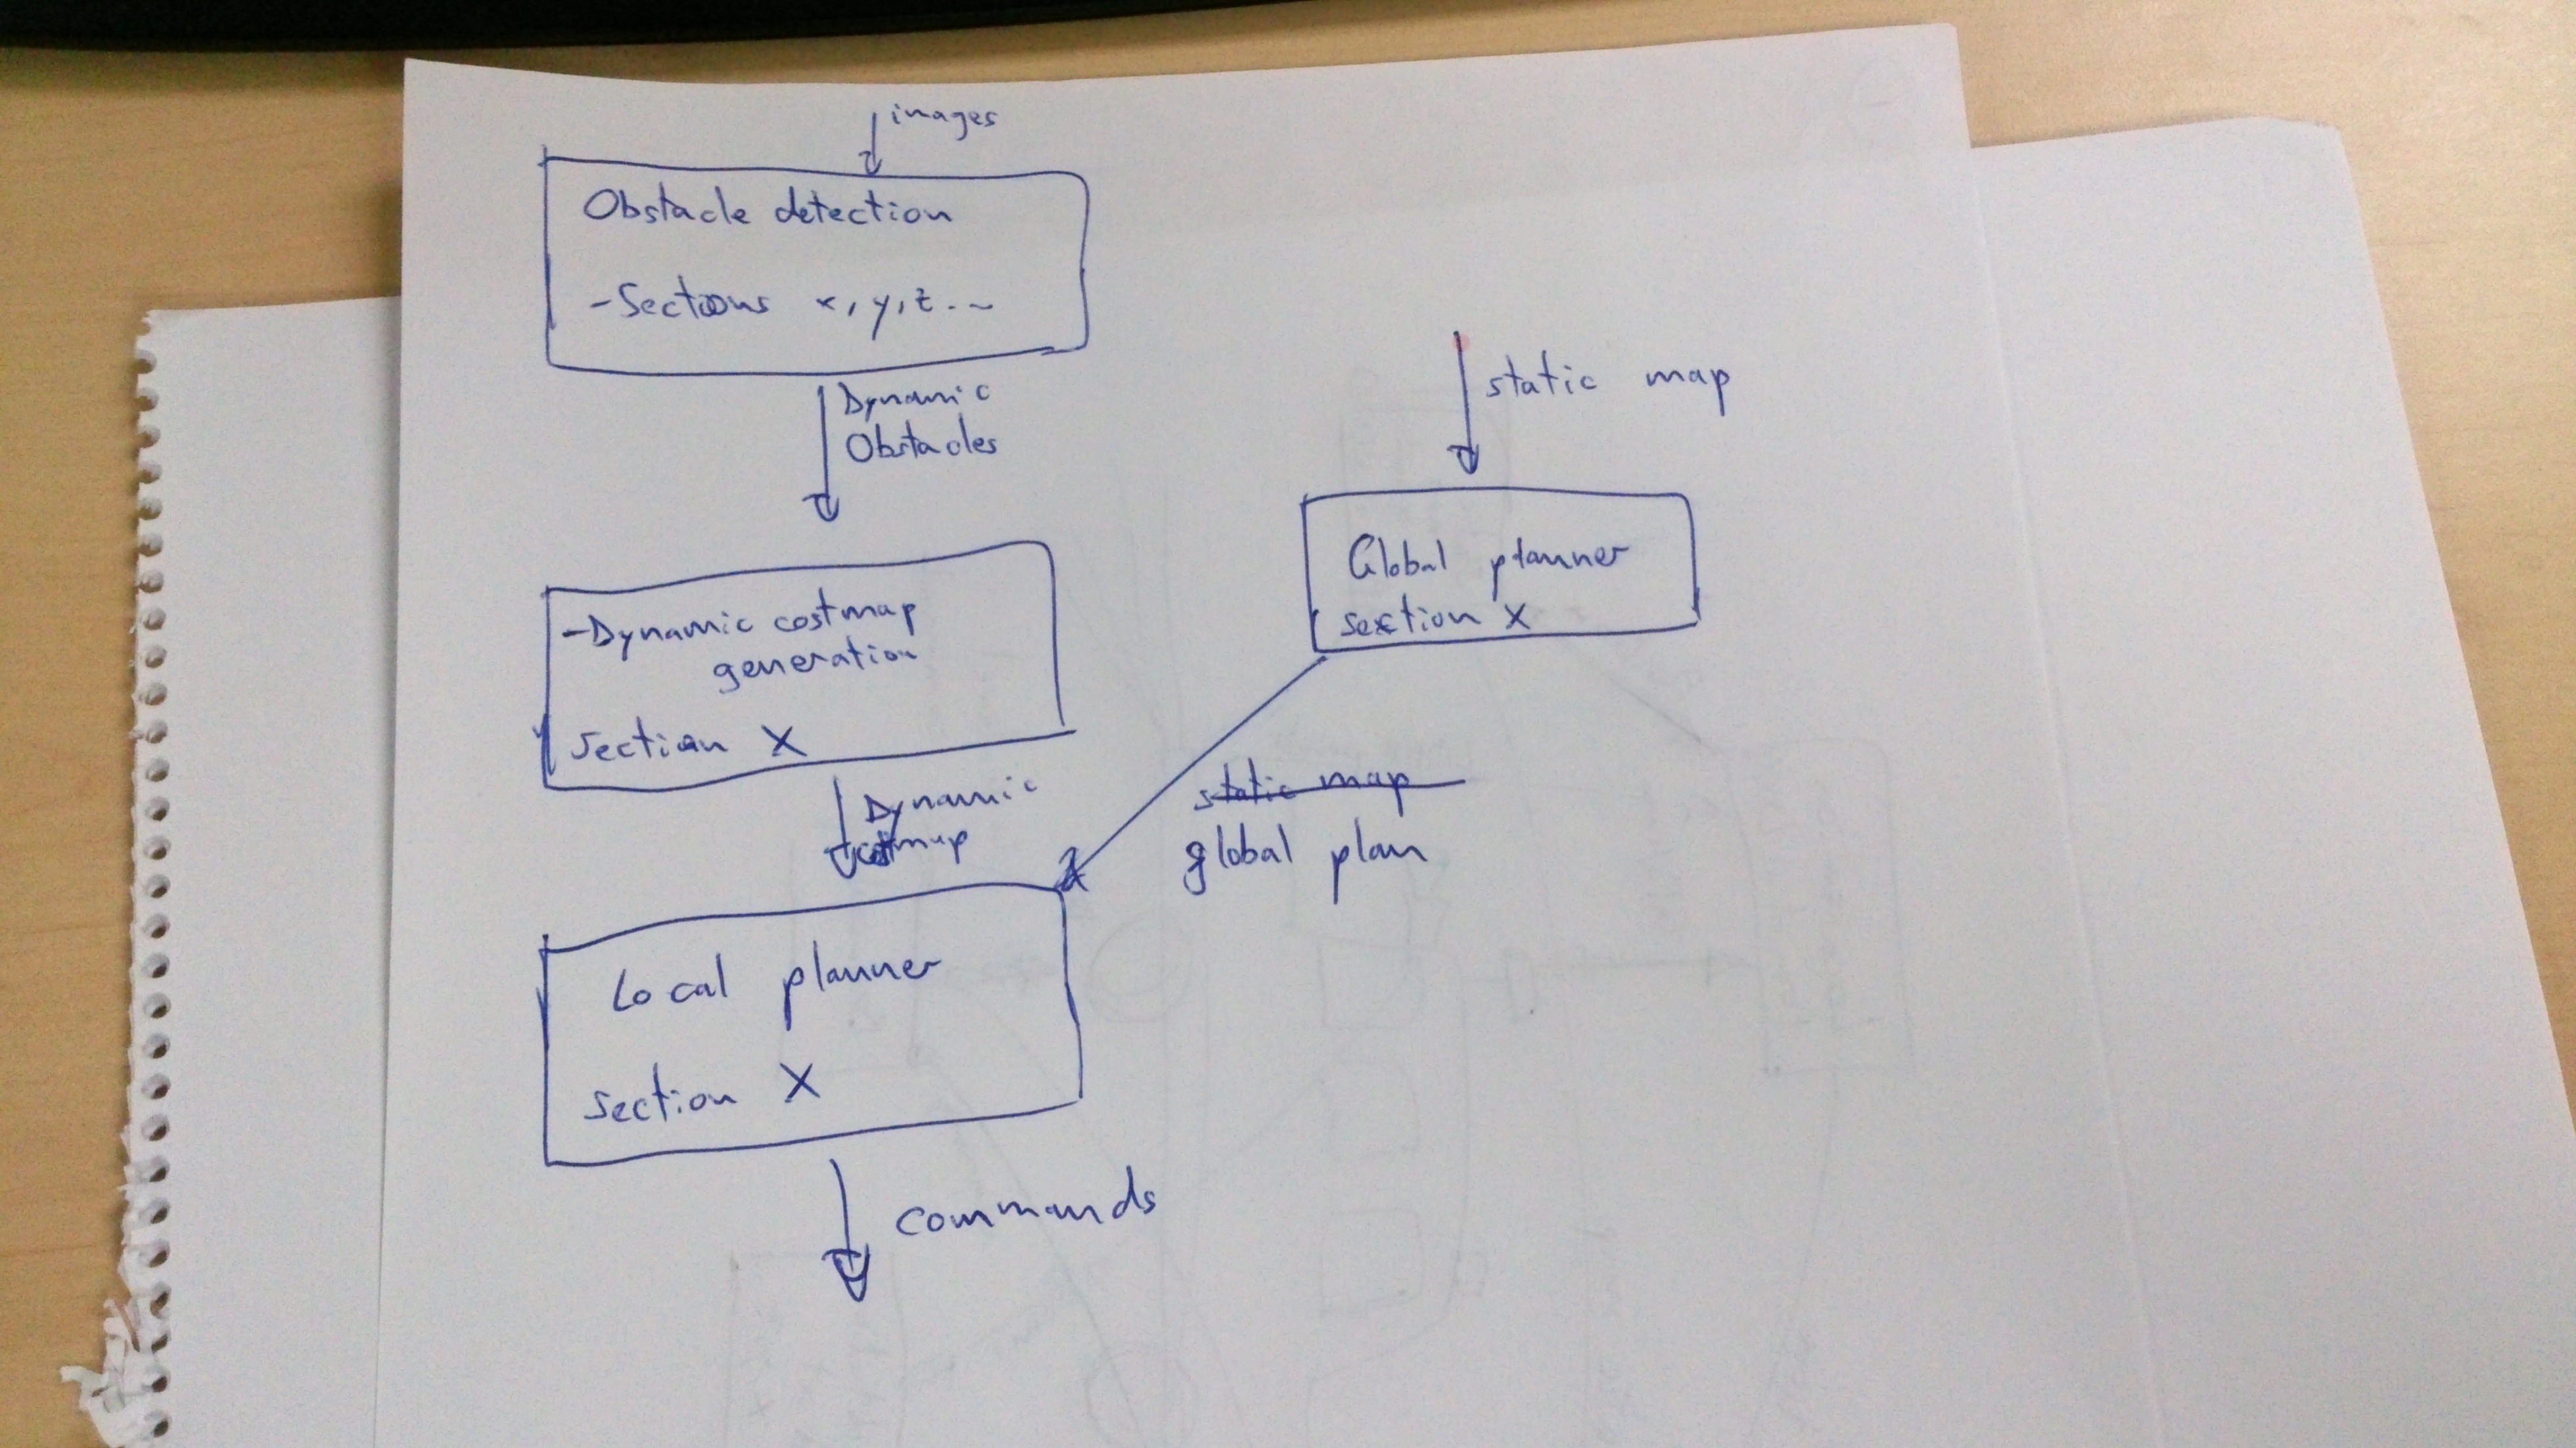
\includegraphics{pipeline}
  \caption{Pipeline of the modules described in this Thesis.}
\end{figure}

From the images captured in real-time, obstacles are located and passed to the module in charge of the generation of the dynamic costmap. At the same time, the static map is used for the generation of a feasible trajectory. Using the current position and vehicle status, the local planner tries to compute the proper commands in order to follow the global plan while trying to avoid the obstacles included in the dynamic costmap.

\section{Previous Work}\label{ch:chapter01_02}

Research on autonomous vehicles is a task being developed for a long time and for which a big effort has been carried on. A proof of that is the extensive literature existing about that topic, in special since the first of the DARPA Challenges (\cite{Buehler2007, Buehler2009}). Since then, the literature related to the topic has increased. Also, the interest on the use of Computer Vision in autonomous vehicles is growing, due to the possibilities that images offer when compared to other sensors, like \acp{LIDAR}.
In 1996, the ARGO project... \todo{Continuar desde aquí, una vez tenga una especie de historia de los vehiculos autonomos, en la intro.}
\todo{TerraMax, VIAC, Braive, Annieway y cualquier otro que pille por el camino.}
As depicted from section \ref{ch:chapter01_01}, the topics described in this thesis are quite diverse, so it is fair to review the state-of-the art of each of these topics separately.

\subsection{Change detection for obstacle localization in images}\label{ch:chapter01_02_01}

\todo{blah blah blah blah blah blah blah blah blah blah blah blah blah blah blah blah blah blah blah blah blah blah blah blah blah blah blah blah blah blah blah blah blah blah blah blah blah blah blah blah blah blah blah blah blah blah blah blah blah blah blah blah blah blah blah blah blah blah blah blah blah blah blah blah blah blah blah blah blah blah blah blah blah blah blah blah blah blah blah blah blah blah blah blah blah blah blah blah blah blah blah blah blah blah blah blah blah blah blah blah blah blah blah blah blah blah blah blah blah blah blah blah blah blah blah blah blah blah blah blah blah blah blah blah blah blah blah blah blah blah blah blah blah blah blah blah blah blah blah blah blah blah blah blah blah blah blah blah blah blah blah blah blah blah blah blah blah blah blah blah blah blah blah blah blah blah blah blah }

\subsection{Non-rigid point set registration for obstacle tracking}\label{ch:chapter01_02_02}

\todo{blah blah blah blah blah blah blah blah blah blah blah blah blah blah blah blah blah blah blah blah blah blah blah blah blah blah blah blah blah blah blah blah blah blah blah blah blah blah blah blah blah blah blah blah blah blah blah blah blah blah blah blah blah blah blah blah blah blah blah blah blah blah blah blah blah blah blah blah blah blah blah blah blah blah blah blah blah blah blah blah blah blah blah blah blah blah blah blah blah blah blah blah blah blah blah blah blah blah blah blah blah blah blah blah blah blah blah blah blah blah blah blah blah blah blah blah blah blah blah blah blah blah blah blah blah blah blah blah blah blah blah blah blah blah blah blah blah blah blah blah blah blah blah blah blah blah blah blah blah blah blah blah blah blah blah blah blah blah blah blah blah blah blah blah blah blah blah blah }

\subsection{Evaluation of stereo 3D reconstruction algorithms}\label{ch:chapter01_02_03}

\todo{blah blah blah blah blah blah blah blah blah blah blah blah blah blah blah blah blah blah blah blah blah blah blah blah blah blah blah blah blah blah blah blah blah blah blah blah blah blah blah blah blah blah blah blah blah blah blah blah blah blah blah blah blah blah blah blah blah blah blah blah blah blah blah blah blah blah blah blah blah blah blah blah blah blah blah blah blah blah blah blah blah blah blah blah blah blah blah blah blah blah blah blah blah blah blah blah blah blah blah blah blah blah blah blah blah blah blah blah blah blah blah blah blah blah blah blah blah blah blah blah blah blah blah blah blah blah blah blah blah blah blah blah blah blah blah blah blah blah blah blah blah blah blah blah blah blah blah blah blah blah blah blah blah blah blah blah blah blah blah blah blah blah blah blah blah blah blah blah }

\subsection{Stixel World}\label{ch:chapter01_02_04}

\todo{blah blah blah blah blah blah blah blah blah blah blah blah blah blah blah blah blah blah blah blah blah blah blah blah blah blah blah blah blah blah blah blah blah blah blah blah blah blah blah blah blah blah blah blah blah blah blah blah blah blah blah blah blah blah blah blah blah blah blah blah blah blah blah blah blah blah blah blah blah blah blah blah blah blah blah blah blah blah blah blah blah blah blah blah blah blah blah blah blah blah blah blah blah blah blah blah blah blah blah blah blah blah blah blah blah blah blah blah blah blah blah blah blah blah blah blah blah blah blah blah blah blah blah blah blah blah blah blah blah blah blah blah blah blah blah blah blah blah blah blah blah blah blah blah blah blah blah blah blah blah blah blah blah blah blah blah blah blah blah blah blah blah blah blah blah blah blah blah }

\subsection{3D object tracking}\label{ch:chapter01_02_05}

By processing the data captured by sensors, it is desired to obtain the position, speed and size of an obstacle. However, usually sensors don't provide this information, so we need to process the information over time and do the tracking of detected obstacles. Many approaches that try to solve this problem, like \cite{danescu2012particle}, assume that obstacles have an standard geometry, and they are modeled as cuboids with associated position, size and speed vectors. This assumption is mostly correct in environments like highways, country roads, and certain urban scenarios, in which almost all the obstacles are cars, trucks or buses which can be simplified as cuboids. Also, these approaches tend to consider a flat ground.
However, this assumption cannot always done, as happens in pedestrian areas, intersections, off-road... In this case, we need to deal with specific shapes, sometimes with concave surfaces. The problem with this kind of obstacles is that methods that assume cuboid-shaped objects tend to wrap the obstacles with a convex shape, which causes an overestimation of their volume (\cite{broggi2013}). Another problem are those objects that are not laying on the ground, as happens with hanged traffic lights, tree crowns, lamps, etc. Usually, they are integrated into an occupancy grid as if they were touching the ground. About the ground plane assumption, in cases like that of an off-road scenario, it is important to estimate the real slope of the road in order to get good results.
Based on how much information they use, we can divide object tracking methods into two subcategories:
\begin{itemize}
 \item \emph{2.5D Solutions:} They do not make use of the complete information provided by 3D points. Instead of that, they tend to use elevation maps composed of uniform size cells. Each cell just stores occupancy and height information. This is the kind of methods that, as described before, usually consider obstacles as being in contact with a flat ground.
 In these methods, tracking is done before the complete reconstruction is done, in an intermediate point based on an specific feature. Based on this intermediate feature, we can distinguishing different kind of approaches:
  \begin{enumerate}
   \item \emph{Use of the 3D point as feature.} An example of this is the so called 6D vision (\cite{franke20056d}), in which the 3D stereo vision extracted information is combined with an efficient implementation of an optical flow in the image space based on a \acf{GPU}. Relevant points are tracked using a Kalman filter.
   \item \emph{Dynamic stixels.} \todo{This approach has been longer discussed in section \ref{ch:chapter01_02_04}.}\comment{Cambiar en caso de que al final no meta los stixels}
   \item \emph{Tracked image features.} As example, check the work by \cite{barth2009estimating}. In this work, obstacles are represented as a rigid 3D point set which are tracked in terms of feature displacements and depth measurements.
   \item \emph{Sensor fusion.} \cite{wu2009collision} reconstruct the objects as cuboids from a stereo point cloud. In this process, position and speed values are improved to a very accurate value by the use of a radar along with stereo.
   \item \emph{Occupancy grids.} This is a very popular choice for tracking. An occupancy grid is a probabilistic map of the driving environment, which encodes the past and present knowledge from sensor data, and which can be updated dynamically when new information is available. These occupancy grids can be cartesian, with rectangular cells, polar, or even a relation between columns in an image an the disparity. An example of this is the method by \cite{danescu2012particle}, which has inspired part of the work described in section \todo { \ref{XXX}}.
   Another advantage of the model based on an occupancy grid is that it makes easier a collaborative update of the grid, which allows the usage of data from several sensors and observers.
  \end{enumerate} 
 \item \emph{3D Solutions:} Usually based on complex grid maps that use complete 3D information. Again, depending on how this grid is represented, we find 
 \begin{enumerate}
   \item \emph{Octree connected cubes.} An example is the work by \cite{wurm2010octomap} or \cite{broggi2013}.
   \item \emph{Adjacent stacks of cells}, as described in \cite{Moravec96robotspatial} 
 \end{enumerate}
\end{itemize}

\subsection{Global planning}\label{ch:chapter01_02_06}

Muchos estudios se han realizado en torno al problema de generacion de rutas globales. Aunque fue inicialmente propuesta para aplicaciones en robotica, ultimamente se ha usado con exito en aplicaciones de automocion.

Podemos dividir los algoritmos de planificacion en... (El resto esta en la libreta, en la parte de estado del arte de planificacion local)


==============================================================
Lo que pongo a continuacion va para la intro de global planning
Los algoritmos de planificacion pueden ser divididos en locales y globales:
Globales:
  La ruta global y los estados del vehiculo quedan determinados por la info proporcionada por un mapa digital y un sistema de localizacion
Locales:
  La ruta local puede ser generada entonces en la etapa de planificacion basada en la ruta global y la info del entorno del vehiculo obtenida por los sensores
  El paper se basa en local path planning que proporciona capacidades de evitacion de obstaculos a un vehiculo autonomo que sigue una ruta global predefinida


\subsection{Local planning}\label{ch:chapter01_02_03}

Con una ruta global calculada y el conocimiento del entorno del vehículo, hace falta enviar al vehículo una serie de comandos que le indiquen cómo seguirla.

En la literatura, muchos métodos se basan en la búsqueda de trayectorias que hagan de intermediarias entre esta ruta global y la ruta local.

Muchos de estos métodos de generación trayectorias se basan en un esquema de optimización discreta (refs. 6, 17-19 coreanos)

Estos métodos calculan un cjto finito de trayectorias basadas en un modelo parametrico, habitualmente funciones polinomiales de un orden determinado. El problema de esto es que a pesar de q el espacio de sol. se reduce y permite una planificacion eficiente, puede introducir suboptimalidad -> Puede llevar a overshoots y/o stationary offsets en curvas

Algunos ejemplos:
(9-annieway) -> Un árbol de trayectorias es muestreado simulando el closed loop system empleando el RRT algorithm
(10-annieway) -> El sistema incorpora varias heurísticas en forma de sampling biases to assert well behaved operation
(17-annieway) El control optimo de un sistema aerodinamico se encuentra dentro de un function space que es spanned by a Garlekin based
Algunos metodos que se basan en la transformacion del espacio de configuraciones mediante el espacio de Frenét:
(Annieway -> Optimal Trajectory Generation for Dynamic Street Scenarios in a Frenét Frame) -> Realiza objetivos a largo plazo como mantenimiento de velocidad, merging, following, stopping por medio de estrategias de ctrol optimo within the Frenét-frame de la calle.
(Stanley: The robot that won the DARPA Grand Challenge) -> Define el offset lateral como la perpendicular a una trayectoria base establecida
  Esta condicion permite al vehiculo circular por la carretera paralelo a la trayectoria base.
  Para seleccionar el path optimo, la funcion de coste penaliza el paso sobre obstaculos y la distancia respecto al centro de la carretera actual
(Coreanos) Tambien genera paths candidatos con endpoints en posiciones fijadas a diferentes offsets respecto al base frame
  Sin embargo, no se basa en el centro de la carretera sino que usa un coste de seguridad para cada path candidato, ya que la estimacion del centro de la carretera puede ser peligroso a la hora de calcular el coste en ciertos escenarios.
  La seguridad de cada path es evaluada cuantitativamente blurring los datos binarios para una colision
  Tb tienen en cuenta como criterios de coste la suavidad y la consitencia del path



\section{Summary}\label{ch:chapter01_03}

In this chapter, we have described a general idea of the work presented in this Thesis. Also, the pipeline of the final developed application is introduced. All this information will be explained in more detail in the following sections, including implementation details together with some results and a discussion of the advantages/disadvantages of the different methods.


% %%
%%  chapter02.tex - Obstacle Detection and Planning for Autonomous Vehicles based on Computer Vision Techniques
%%
%%  Copyright 2014 Néstor Morales <nestor@isaatc.ull.es>
%%
%%  This work is licensed under a Creative Commons Attribution 4.0 International License.
%%

\graphicspath{{./images/chapter02/bmps/}{./images/chapter02/vects/}{./images/chapter02/}}

\chapter{Change detection for obstacle localization in images}\label{ch:chapter02}


\graphicspath{
  {./images/bmps/}{./images/vects/}{./images/}
  {./images/presentation/bmps/}{./images/presentation/vects/}{./images/presentation/}
  {./images/chapter00/bmps/}{./images/chapter00/vects/}{./images/chapter00/}
  {./images/chapter03/bmps/}{./images/chapter03/vects/}{./images/chapter03/}
}

\subsection{Evaluation of Stereo 3D Reconstruction Algorithms}
\begin{frame}{Introduction}
  \begin{itemize}
    \item We want to know the best performance algorithms available for environmental mapping.
    \item Very few datasets $\rightarrow$ Most of them in controlled conditions
    \item Three different dense reconstruction algorithm implementations
    \item Three different and well-known evaluation strategies
  \end{itemize}
  
  \note {
  \begin{itemize}
   \item Critical tasks in the development of driving assistance systems and stereo vision has been widely used to accomplish it
   \item that allow assessing the performance of a specific method in a real world application
   \item conditions... which are not able to capture the variety of the real world
   \item These strategies represent a trade-off btween cost, set up time and accuracy
  \end{itemize}
  }
\end{frame}

\begin{frame}{Introduction}
  Little o no data available to be used as ground truth.
  \begin{itemize}
    \item<1-> Use of a high-end LIDAR (LIgth Detection and Ranging) unit\footnote{\cite{Geiger2012}}.
    \item<2-> Exploit a prior over the data-set\footnote{\cite{Steingrube2009}}.
    \item<3-> Synthesize a virtual view\footnote{\cite{Morales2009}}.
  \end{itemize}
  \begin{overlayarea}{\textwidth}{0.5\textheight}
    \only<2>{
    \begin{exampleblock}{Example}
      The presence of freespace in front of a manually driven vehicle to detect wrongly reconstructed points.
    \end{exampleblock}
    }
    \only<3>{
    \begin{exampleblock}{Example}
      A virtual view synthesized from the reconstructed environment geometry can be compared with the actual data recorded from a third camera.
    \end{exampleblock}
    }
  \end{overlayarea}
  
  \note {
  }
\end{frame}

\begin{frame}{Experimental setup}
  \framesubtitle{Dense LIDAR-based ground truth}
  \begin{itemize}
    \item KITTI dataset from the Karlsruhe Institute of Technology.
    \item Only non-occluded computed pixels have been considered
    \item Average errors have been computed considering only the values below the endpoint error.
    \item Statistics for each frame are being considered, not just their average over an entire sequence.
  \end{itemize}
  
  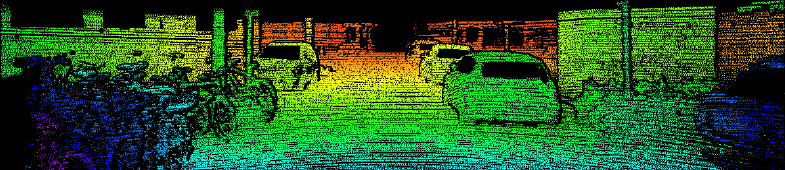
\includegraphics[width=\textwidth]{lidarGT}

  \note {
  \begin{itemize}
    \item Ground truth for a given frame is obtained by registering 5 consecutive frames before and after the one selected and accumulating the resulting point clouds.
    \begin{itemize}
      \item Ambiguous regions such windows and fences are manually removed
      \item The corresponding disparity map is computed using calibration information
    \end{itemize}
    \item The original benchmark also uses linear interpolation of missing values, making sparse and semi-dense methods comparable to dense ones -> This is not fair and hardly optimal // Worsened error metrics for non-dense algorithms.
    \item ... And not all the values
    \item To better understand the collected data, it will be plotted in a graph with the independent variable (x-axis) representing the measured value, and the dependent one (y-axis) the percentage of frames falling below it. Better-performing algorithms are those with a lower x value for a given frame percentage (e.g. y = 90%).
 \end{itemize}
 }
\end{frame}

\begin{frame}{Experimental setup}
  \framesubtitle{False correspondences estimation}
  \begin{itemize}
    \item A safety distance of about 1\,s is usually kept from a leading vehicle.
    \item A speed-dependent free volume is present in front of the ego-vehicle. \\
  \end{itemize}

  \begin{center}
    \begin{figure}[t]
	  \centering
	  \begin{subfigure}[t]{0.5\textwidth}
	      \includemovie[autoplay, repeat]{\linewidth}{0.5\textheight}{/home/nestor/Seafile/Videos/Tesis/cp03/FC.avi}
	  \end{subfigure}% 
	  ~
	  \begin{subfigure}[t]{0.5\textwidth}
	      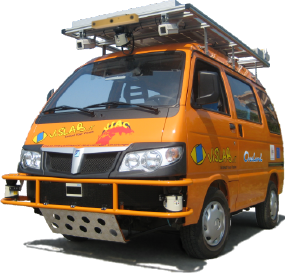
\includegraphics[height=0.5\textheight]{viac_van}
	  \end{subfigure}%       
    \end{figure}
  \end{center}

  \note {
    \begin{itemize}
     \item Any reconstructed point falling within said area must be considered as an erroneous estimate.
     \item We reject false negatives using the LIDAR information.
     \item Face correspondences percentage is the ratio of points inside the object-free volume respect to the total number of 3D points.
    \end{itemize}
  }
\end{frame}

\begin{frame}{Experimental setup}
  \framesubtitle{Normalized Cross Correlation (NCC)}

  \begin{center}
    \begin{figure}[t]
	  \centering
	  \begin{subfigure}[t]{0.5\textwidth}
	    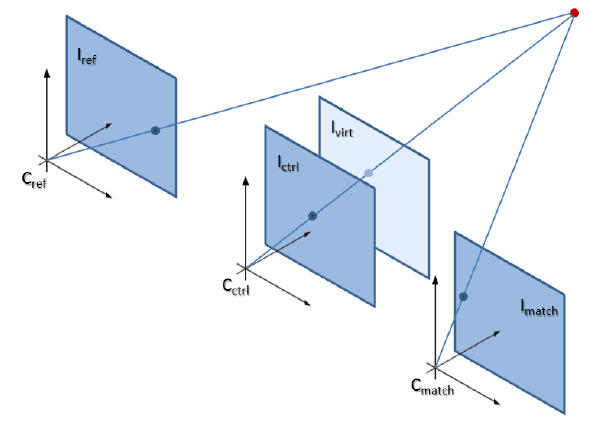
\includegraphics[width=\textwidth]{trinocular_setup}
	  \end{subfigure}% 
	  ~
	  \begin{subfigure}[t]{0.5\textwidth}
	    \includemovie[autoplay, repeat, controls]{\linewidth}{0.5\textheight}{/home/nestor/Seafile/Videos/Tesis/cp03/ncc.avi}	      
	  \end{subfigure}%       
    \end{figure}
  \end{center}

  \note {
    \begin{itemize}
     \item LIDAR-based GT takes time to be produced and FC is an indirect measurement.
     \item The use of a third camera allows to directly compare a reconstructed view with the actual images w/o manual intervention.

     \item NCC is calculated as described by Morales et al.

     \item It is suggested a configuration of 20 cm btween ref and match, and the ctrol camera is at 50 cm from ref camera
     \item In our conf, it is 24 and 12, respectively, as we use a precalibrated trinocular camera.
    \end{itemize}
  }
\end{frame}

\begin{frame}{Algorithms}
  Three dense reconstruction algorithms tested:
  \begin{itemize}
   \item Census Cost Semi-Global Matching (Census-SGM) \footnote{\cite{Hirschmuller2005, Hirschmuller2009}}
   \item Birchfield-Tomasi Semi-Global Matching (BT-SGM)\footnote{\cite{Hirschmuller2005, Birchfield1998}, \url{http://opencv.org}}
   \item Efficient Large-Scale Stereo Matching (ELAS) \footnote{\cite{Geiger2011}}
  \end{itemize}


  \note {
    \begin{itemize}
     \item LIDAR-based GT takes time to be produced and FC is an indirect measurement.
     \item The use of a third camera allows to directly compare a reconstructed view with the actual images w/o manual intervention.

     \item NCC is calculated as described by Morales et al.

     \item It is suggested a configuration of 20 cm btween ref and match, and the ctrol camera is at 50 cm from ref camera
     \item In our conf, it is 24 and 12, respectively, as we use a precalibrated trinocular camera.
    \end{itemize}
  }
\end{frame}

\begin{frame}{Algorithms}
  \framesubtitle{Semi-Global Matching}
  
  \begin{itemize}
    \item Disparity search range is reduced
    \begin{itemize}
      \item A set of sparse, robustly matched control points is found.
      \item A 2D mesh is generated via Delaunay triangulation.
      \item A prior is created from this mesh
    \end{itemize}
  \end{itemize}

  \note {
    By computing a piecewise linear function induced by the support point disparities and the triangulated mesh.
  }
\end{frame}

\begin{frame}{Algorithms}
  \framesubtitle{Efficient Large-Scale Stereo Matching (ELAS)}
  
  \begin{itemize}
    \item Gets the disparity map D by minimizing \\
    \begin{center} $E(D) = E_{data}(D) + E_{smooth}(D)$ \end{center}
    \item NP-complete (but tractable using DP).
    \item Two cost metrics:
    \begin{enumerate}
      \item Census cost metric.
      \begin{itemize}
	\item Hamming distance of the Census transform of a 5x5 window.
      \end{itemize}
      \item  Birchfield-Tomasi cost metric.
    \end{enumerate}
  \end{itemize}

  \note {
    \begin{itemize}
     \item $E_{data}$ is the pixel-wise matching cost
     \begin{itemize}
      \item Sum of all pixels matching costs for the disparities of D
     \end{itemize}
     \item $E_{smooth}$ is the smooth constraint.
     \begin{itemize}
      \item adds a small penalty P1 to all px in the neighborhood of a pixel p for which the disparity varies by one
      \item adds a higher penalty P2 if greater
     \end{itemize}
     \item SGM is no tractable in real time, unless we use a DP strategy
     \item each pixel is used as the px-wise matching function, instead of the mutual information, as used in the original implementation.
     \item Similar results, but reduces the overall processing burden
     \item Each position C(p, d) of the cost volume is initialized with the number of differing bits btween the corresponding transformed values of left-right images.
     \item We have used the freely available OpenCV implementation that uses BT pixel dissimilarity as cost metric to initialize the cost
    \end{itemize}
  }
\end{frame}

\begin{frame}{Algorithms}
\begin{table}[h!]
\begin{center}
\resizebox{\columnwidth}{!} {
\begin{tabular}{|l|c|c|c|c|c|}
 \cline{2-6}
 \multicolumn{1}{ c|}{} & \multicolumn{3}{ c| }{Census-SGM} &
 \multicolumn{1}{ c| }{\multirow{2}{*}{BT-SGM}} &
 \multicolumn{1}{ c| }{\multirow{2}{*}{ELAS}} \\ \cline{2-4}
 \multicolumn{1}{c|}{} & Config 1 & Config 2 & Config 3 & & \\ \cline{2-6}
 \hline \hline
 Gaussian filter & $\surd$ & $\surd$ & $\surd$ & - & - \\
 Sparse Census mask & - & - & - & - & - \\
 Ternarized Census & - & - & - & - & - \\
 Hamming scores aggregation  & - & - & - & - & - \\
 Uniqueness constraint & 10 & 20 & 20 & 10 & 15 \\
 Adaptive mean & $\surd$ & $\surd$ & $\surd$ & - & $\surd$ \\
 Despeckle filter & $\surd$ & $\surd$ & $\surd$ & $\surd$ & $\surd$ \\
 Gap filter & $\surd$ & $\surd$ & - & - & $\surd$ \\
 \hline \hline
 Other parameters & \multicolumn{3}{ |c }{$P_1=10$, $P_2=50$, L/R check} &
 \multicolumn{1}{ |c }{see \footnote{\url{http://www.cvlibs.net/datasets/kitti/eval\_stereo\_flow.php}}} &
 \multicolumn{1}{ |c| }{see \footnotemark[\value{footnote}]} \\
 \hline
\end{tabular}
}
\end{center}
\end{table}
\end{frame}

% \graphicspath{{./images/chapter04/bmps/}{./images/chapter04/vects/}{./images/chapter04/}}

\chapter{Stixel World}\label{ch:chapter04}

In the previous chapter, we saw a set of algorithms and configurations able to construct a disparity map from a pair of stereo images. These methods are useful for the reconstruction of the environment. However, this reconstruction is dense, which leads to an intensive usage of the computer resources. In order to solve this problem, some authors propose approaches that try to minimize the area of the image being processed by doing a simpler reconstruction than that done with dense 3D reconstruction algorithms. In this sense, \cite{badino2009stixel} proposed to represent the world by a set of rectangular sticks named \emph{stixels} (from \emph{stick} and \emph{pixel}). Each stixel is defined by its 3D position relative to the camera and stands vertically on the ground, having a certain height.
This compact but flexible representation of the world can be used as the common basis for the scene understanding tasks of driver assistance and autonomous systems. The main advantages of using such an approach are listed next:
\begin{itemize}
 \item \emph{Compact}. Significant reduction of the data volume.
 \item \emph{Complete}. Information of interest is preserved.
 \item \emph{Stable}. Small changes of the underlying data must not cause rapid changes within the representation.
 \item \emph{Robust}. Outliers must have minimal or no impact on the resulting representation.
\end{itemize}

The method described in this chapter is based in the fast stixels implementation described in \cite{benenson2012pedestrian}. One of the main advantages of this implementation is that there is no need of obtaining a previous depth map. This fact is also the main reason for which we did not use the original implementation from \cite{badino2009stixel} or that from \cite{pfeiffer2010efficient}. Based on the output of this method, we do the tracking of the stixels following a bipartite-graph method based on a given cost metric. In this sense, we have tested several cost metrics, which are described in the following sections.

Our tracking method is based on the contribution by \cite{gunyel2012stixels}. There, movement is just computed for the areas which are covered by stixels. It has been demonstrated that stixels are good enough to do a representation of the surroundings of a vehicle, and that they have a detail level enough for the movement detection. Traditionally, this movement detection is carried out through the computation of the optical flow between two frames, which is computationally expensive. In this chapter, we will see how this movement can be computed also using the stixel world representation, by extending the method of \cite{gunyel2012stixels}. For that, we have followed two different approaches, each with its own benefits and drawbacks. The first tries to cluster the stixels in objects, so the tracking is performed at object level; the second joins the stixel tracking with the object tracking in a two level tracking scheme.

Our contribution in this work is summarized next:
\begin{enumerate}
 \item Improvement of the reconstruction obtained by the stixels. The free space computation without the use of a disparity map have some drawbacks. Some of them are related with the fact that the precision in the reconstruction of the obstacles is not good enough. The object reconstruction detection scheme proposed in this chapter allows the correction of the stixel depths and the removal of the fake obstacles, as described in sections \ref{ch:chapter04_02_01} and \ref{ch:chapter04_02_02}.
 \item Improvement of the results obtained by the method described in \cite{gunyel2012stixels}, in both object and two-level tracking approaches. We modified the method by using a graph-based approach instead of a \ac{DP} based method, as they did. 
 \item Different cost metrics for the tracking have been tested, with promising results. 
 \item Faster tracking. As we will see in section \ref{ch:chapter04_02_04}, the speed achieved with our implementation is better, specially in the object based tracking. The two-level tracking is also a little bit faster, thanks to the usage of a bipartite graph based method for the matching of the stixels between frames.
 \item Our method is slightly more robust after changes between images (for example, in presence of a low framerate), specially in the case of the just object based approach.
\end{enumerate}

In the following section, each of the steps of the method are detailed. At the end of the chapter some results are shown in order to evaluate the performance of the described method.

\section{The Method}\label{ch:chapter04_01}

The method follows a pipeline as that described in figure \ref{fig:cp04_pipeline}. First, from a given pair of images, the free space in front of the vehicle is computed in order to estimate the ground plane. From the extracted ground plane, stixels are obtained. Then, a two-level tracking approach is started. The first level is that corresponding to the tracking of the stixels. This stage is inspired by the work described in \cite{gunyel2012stixels}. The set of stixels computed for the current frame are compared with those from the previous frame. Based on this comparison, some of them are matched. At the same time, we cluster stixels based on their position once projected in the 3d world. Using the clusters and the tracked stixels, we start a new tracking step in which the tracking is performed at object level. At the end of this step, we will know the obstacles in the scene and their velocities, as well as an historic of the path followed by them that could be useful for future movement estimation.

We also propose another solution in which just the object level tracking is performed. In this case, instead of doing a comparison at stixel level, we compare each obstacle to the obstacles detected in the previous frame, so the stixel level tracking is not needed anymore. In section \ref{ch:chapter04_02}, we will see the advantages and drawbacks of using one or another approach.

\begin{figure}[h!]
  \centering
  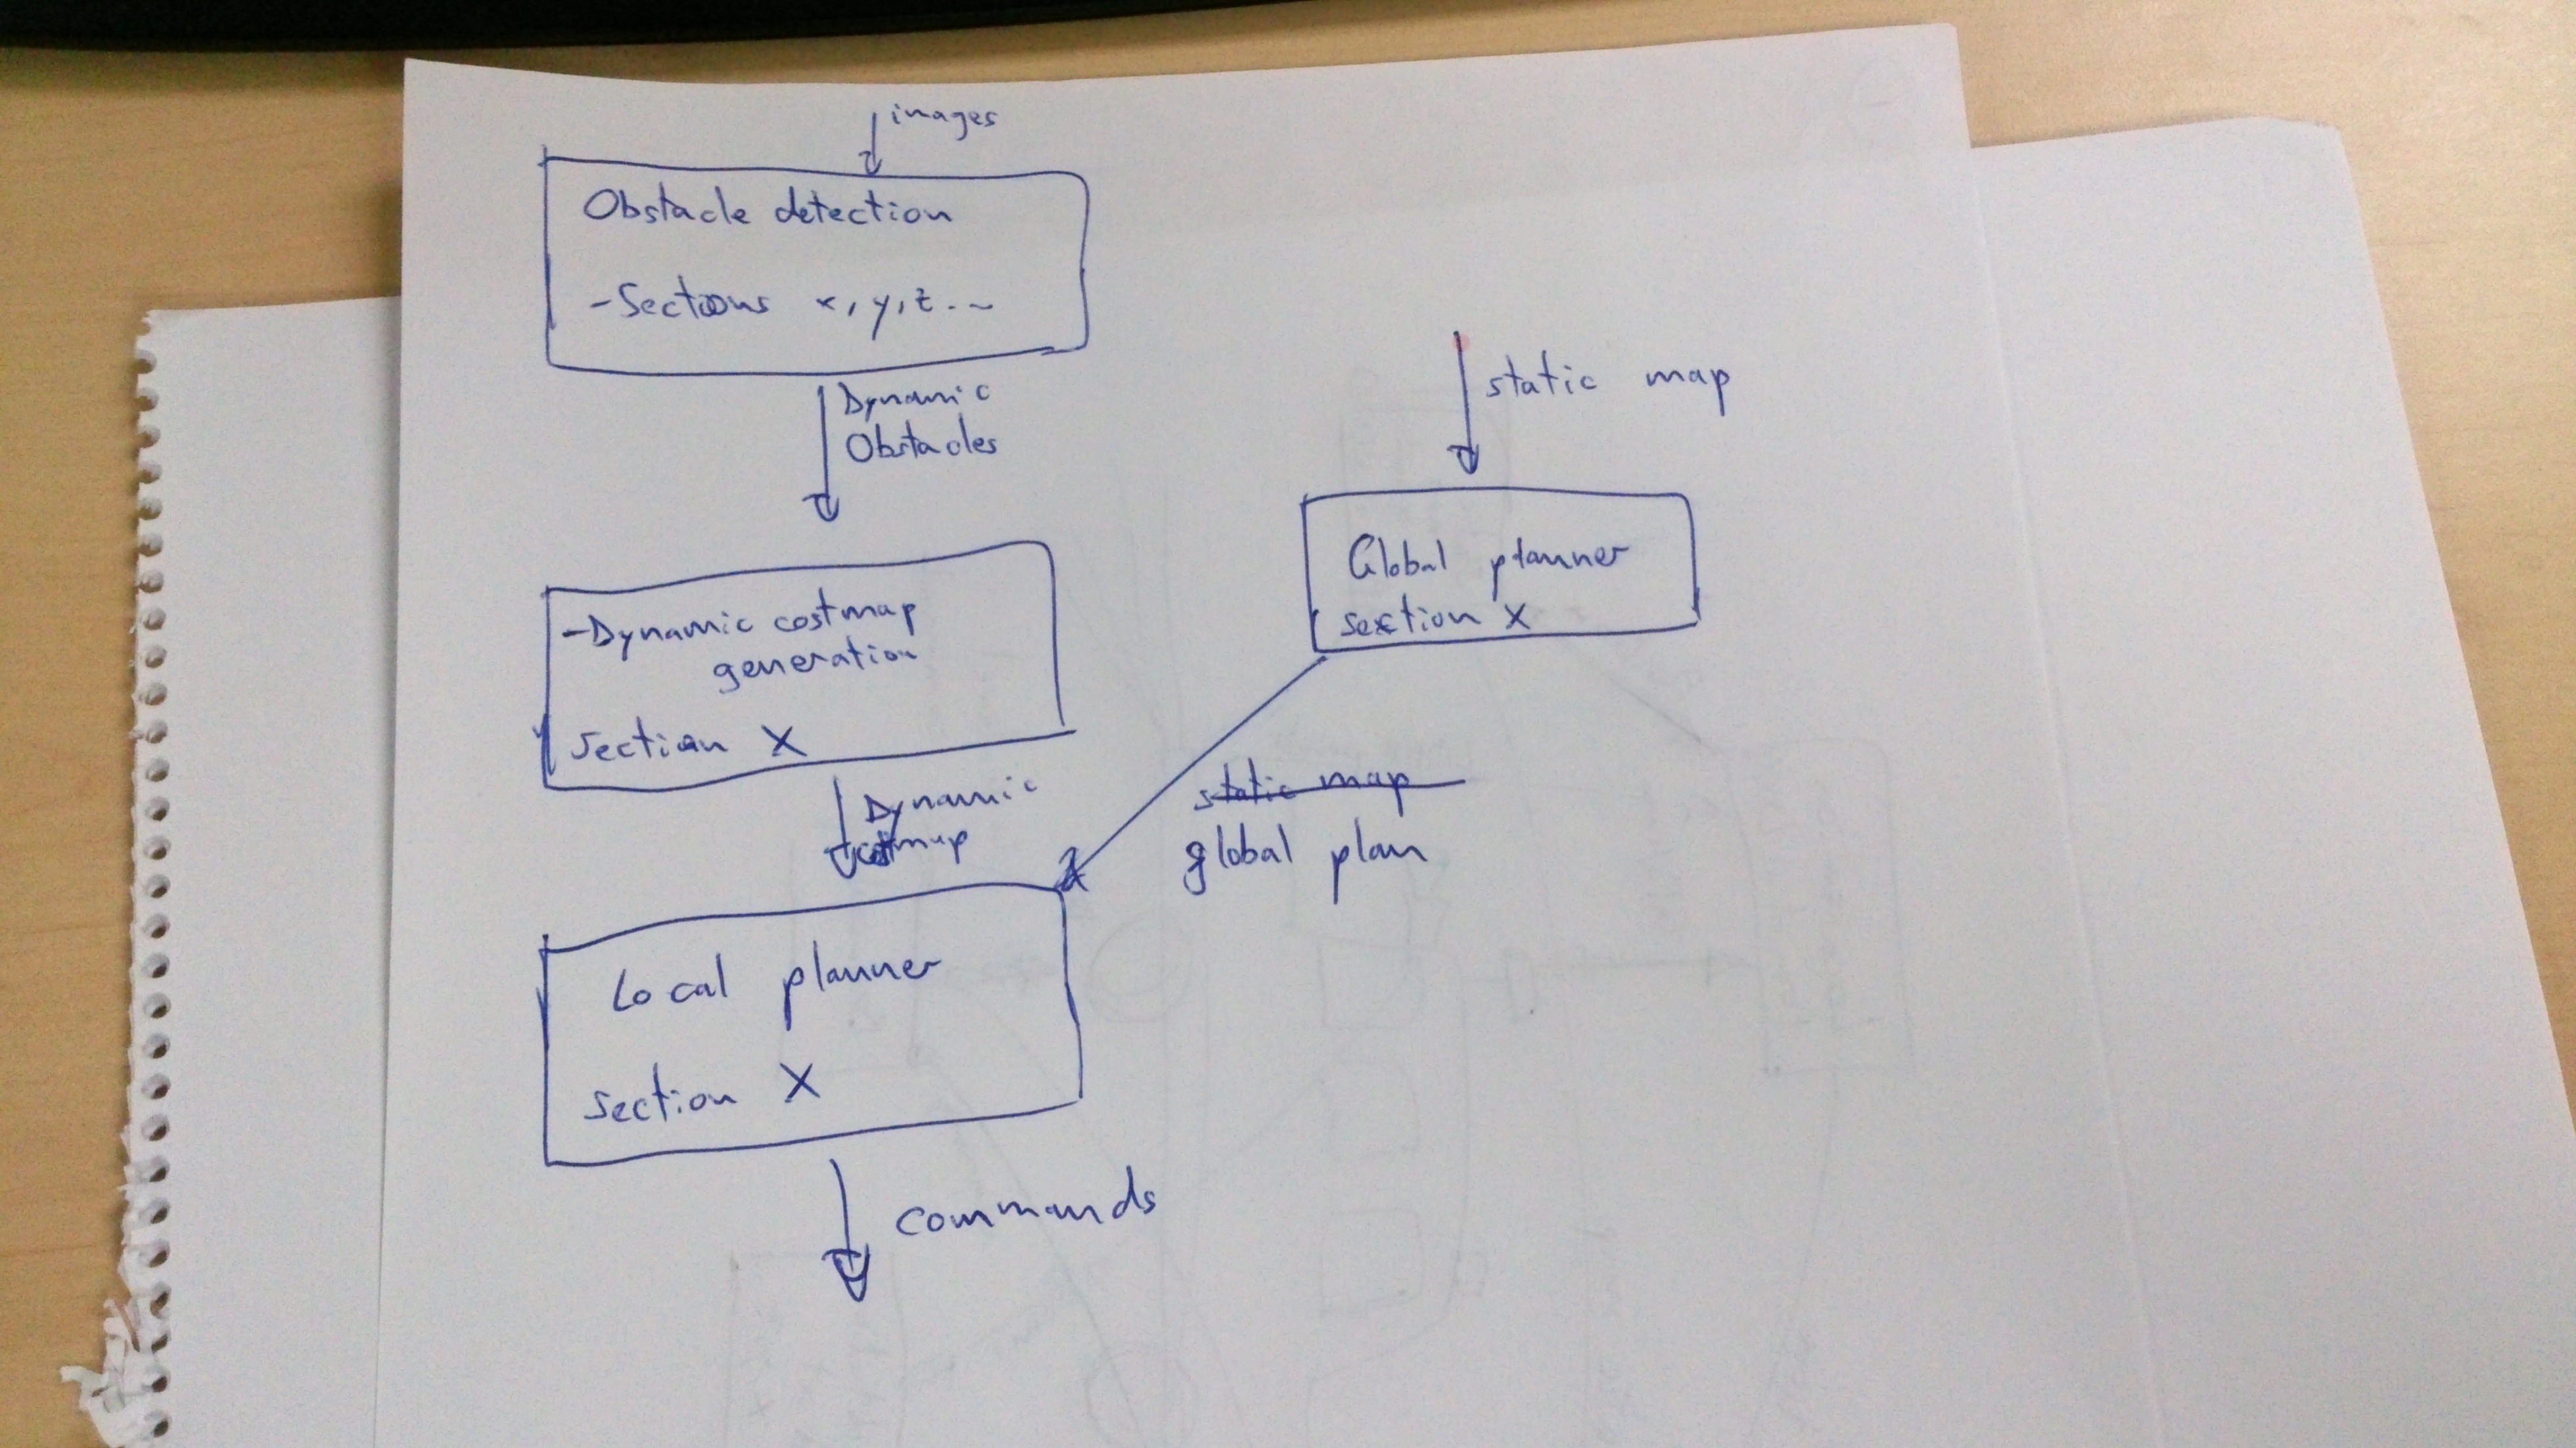
\includegraphics{pipeline}
  \caption{Pipeline of the stixels tracking method described in this chapter.}\label{fig:cp04_pipeline}
\end{figure}

\subsection{Free space computation}\label{ch:chapter04_01_01}

In this section and in the following, we will describe the stixel extraction method, which is similar to that described in \cite{benenson2012pedestrian}. This method works under the following assumptions:

\begin{itemize}
 \item The input of the algorithm is a calibrated stereo image pair.
 \item We use the Lambertian surface assumption.
 \item The ground is planar, at least at local level.
 \item The objects of interest are mainly vertical, and have a limited height range.
 \item Stereo rig has a negligible roll with respect to the ground plane.
\end{itemize}

In this section, we introduce the first step needed for the stixels estimation process, which is the ground plane estimation stage. This ground plane is estimated using the evidences collected in the \emph{v-disparity} domain. Instead of computing and projecting a depthmap obtained, for example, one of the methods evaluated in chapter \todoref{XXX}, the evidence is collected directly from matching the rows from the left and right images at different disparities, obtaining a cube $(U, V, D)$ in which each cell represents the cost of matching the pixel at $p_i(u_i, v_i) \in I_L$ with that at $q_i(u_i + d_i, v_i) \in I_R$. Here, $p_i$ and $q_i$ are pixels from the left ($I_L$) and right ($I_R$) images, respectively; and $u_i$, $v_i$ and $d_i$ are the different possible column, row and disparity values in the cube. In figure \ref{fig:cp04_freespace}, a graphical description of the obtained cube is represented.

\begin{figure}[h!]
  \centering
  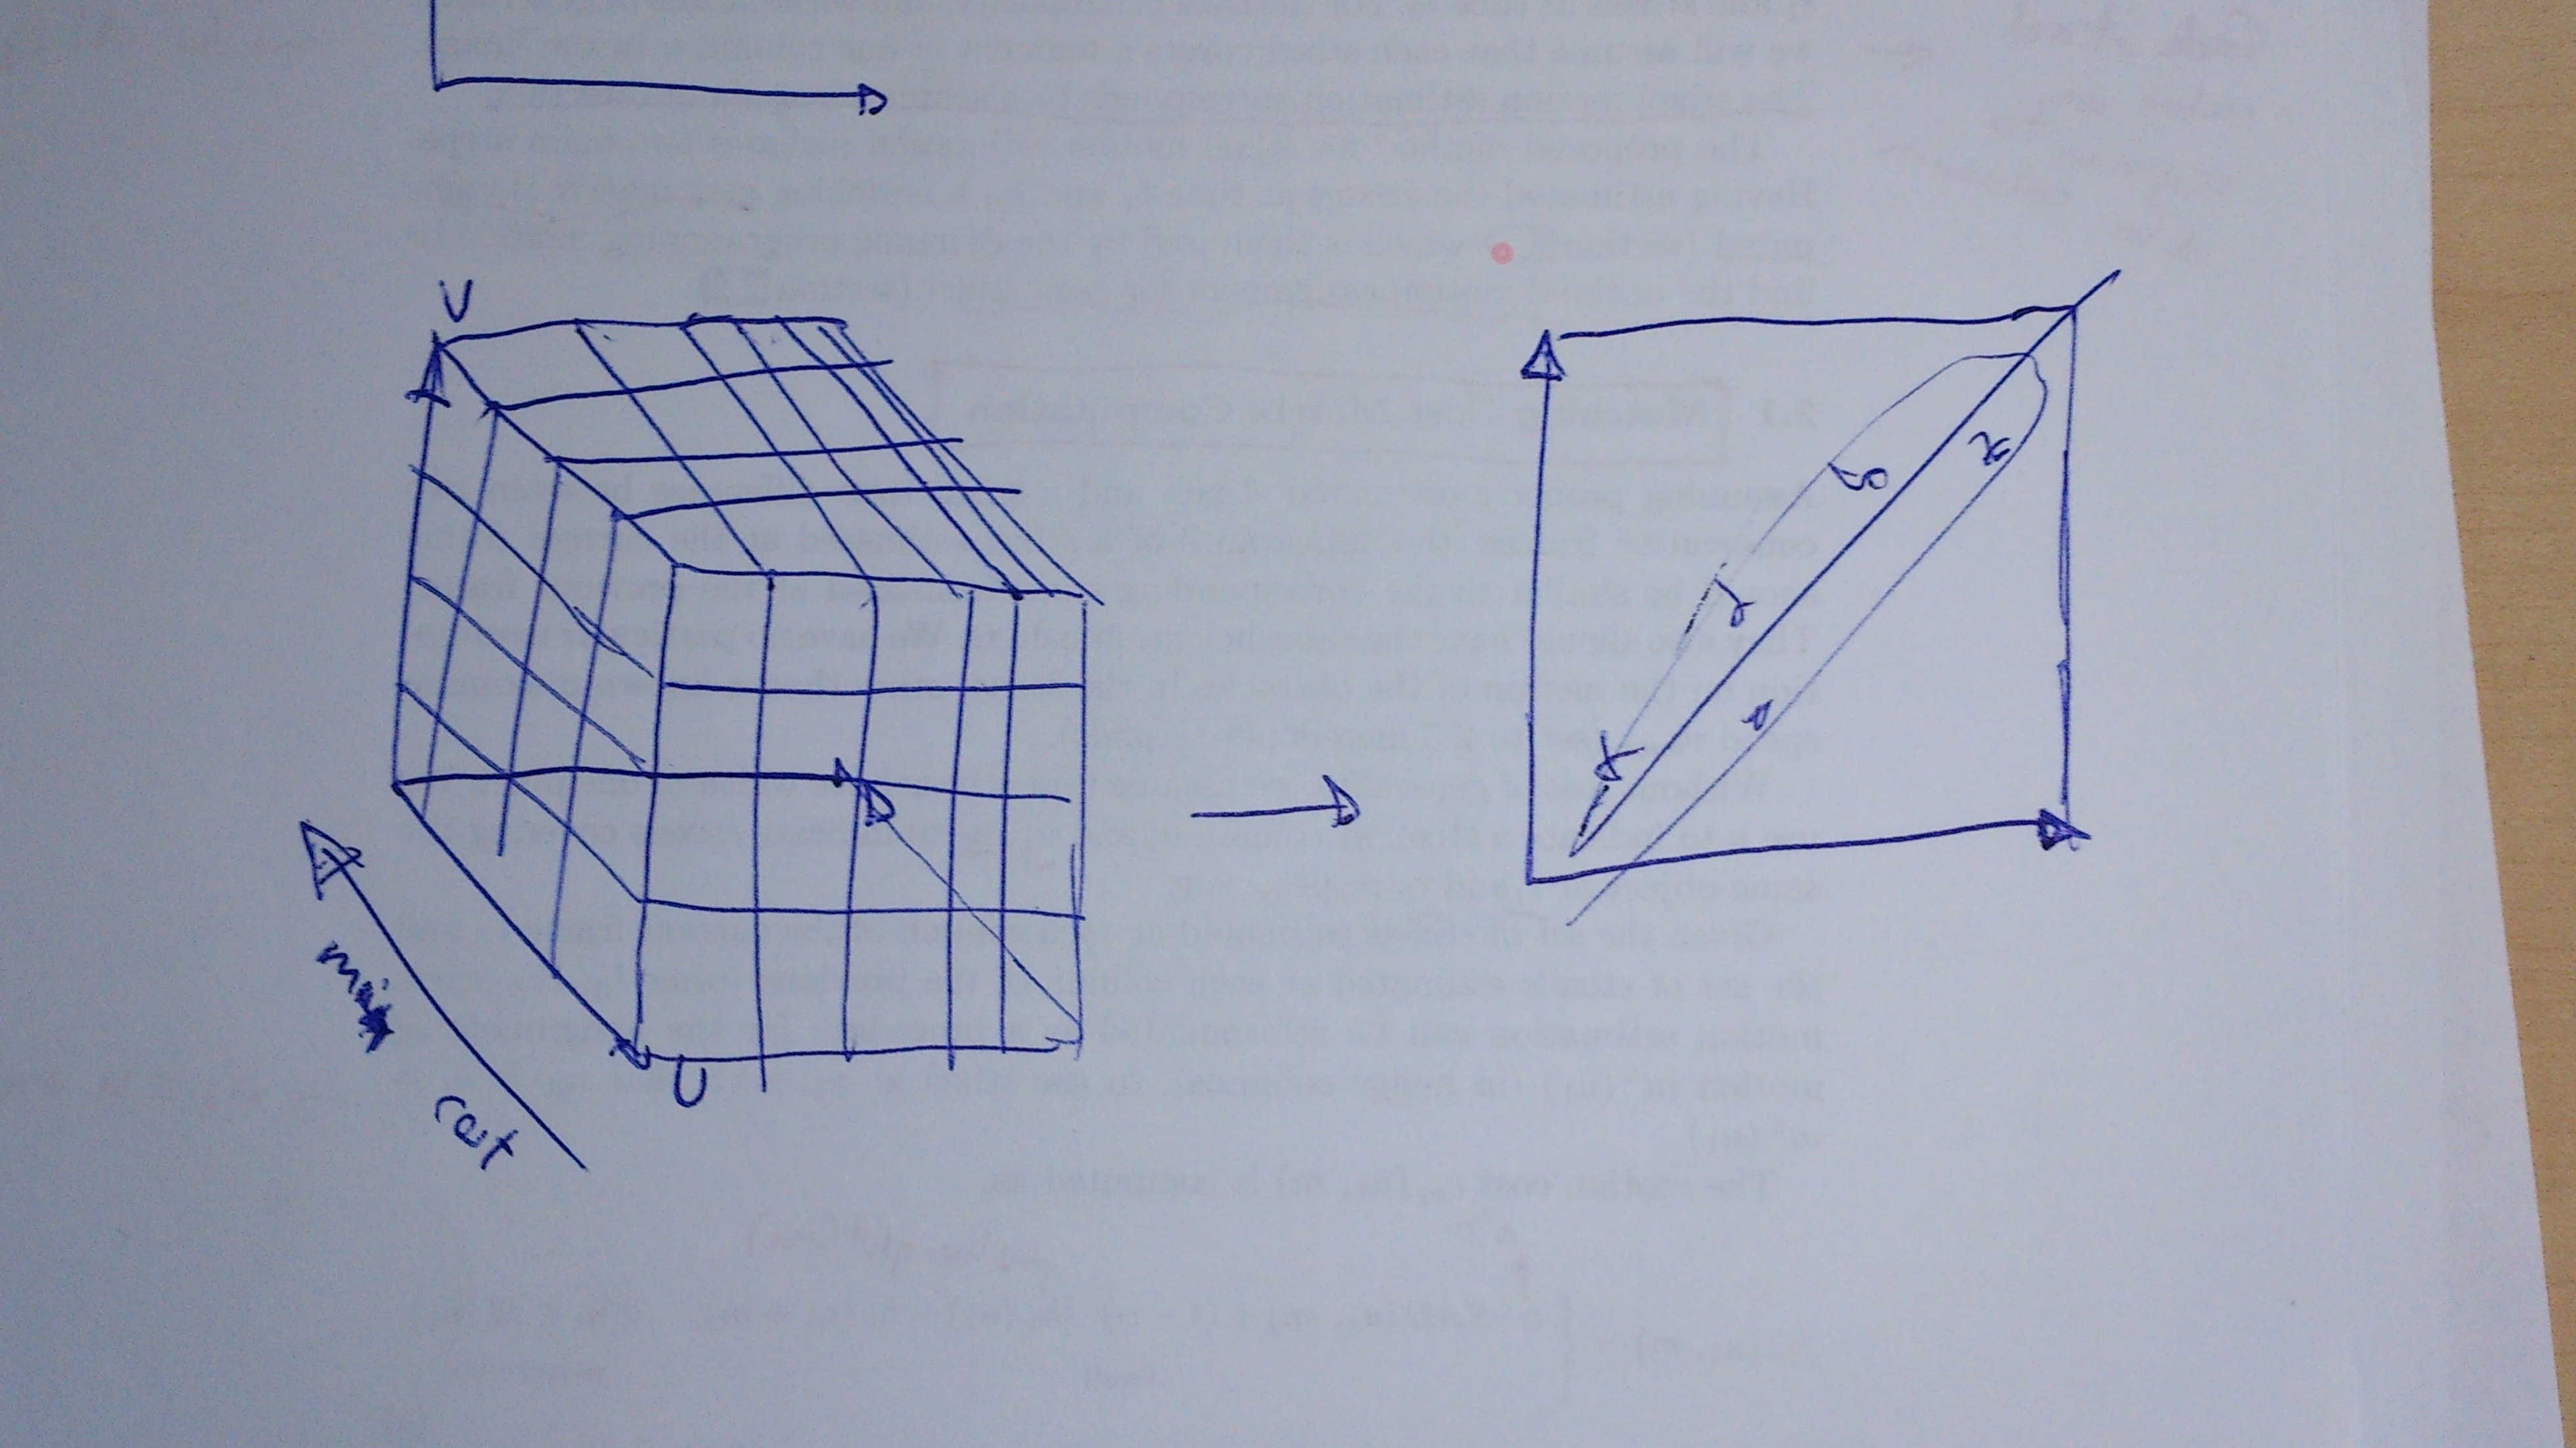
\includegraphics{freespace}
  \caption{Free space computation process.}\label{fig:cp04_freespace}
\end{figure}

For each row $v_i$, the disparity with the lowest cost is extracted for each row, as depicted in figure \ref{XXX}. From these values, a robust line fitting is used in order to find the ground plane, which is represented by the following expression:

\begin{equation}\label{eq:cp04_ground_plane_function}
  d_i = f_{ground}(v_i)
\end{equation}

Using this equation, we can know the disparity associated to each row at ground level, which will we use later for the stixels computation. For optimization purposes, instead of collecting the evidences for each row below the horizon, just one out of each $N$ rows is computed. 

\subsection{Stixels extraction}\label{ch:chapter04_01_02}

With the ground plane, we can start detecting the stixels in the images. The way in which this is done is by dividing the image in multiple row bands $b_i$. Inside each band $b_i$, and for each column $u_i$, the pixel with the biggest horizontal gradient is selected. This reduces the computational cost while the possibilities of finding the border of the object accurately are increased. Also, one of the advantages of using bands and not the rows directly is that, in presence of a confusing horizontal line, the effect is compensated by the band height.

From \ref{fig:cp04_freespace}, we obtain:

\begin{equation}\label{eq:cp04_ground_plane_function_by_band}
  d(q_j, b_i) = f_{ground}(v(q_j, b_i))
\end{equation}

Here, $q_j$ makes reference to the stixel $j$, where the total number of stixels is the total number of columns in the image divided by a parameterized stixel width $\tau_{stixel\_width}$. That is, $j=1 \dots \tau_{stixel\_width}$. In general, interest objects are wider than one column, so computing an evidence for each column in the image is redundant. Each stixel is located in the column $u(q_j) = j \cdot \tau_{stixel\_width}$. $v(q_j, b_i)$ is a certain row inside the stixel $q_j$ in the band $b_i$. 

At this point, the goal is to localize the optimal band for each stixel. This is based on the following expression:

\begin{equation}\label{eq:cp04_stixel_band_cost}
  b^*_s (q) = \underset{b(q)}{\arg\min} \underset{q}{\sum}c_s(q, b(q)) + \underset{q_a, q_b}{\sum}s_s(v(q_a, b(q_a)), v(q_b, b(q_b)))
\end{equation}

Here, we can think on $c_s$ as the data term, while $s_s$ is the smooth term. $q_a$ and $q_b$ are neighbors. That is, $|q_a - q_b| = 1$

\paragraph{Data term}\label{ch:chapter04_01_02_01}

By computing the cost $c_s$, we know the likelihood of the presence of an stixel $q$ at the row band $b$. The lower the cost is, the more possible that there is a stixel. This cost is computed as follows:

\begin{equation}\label{eq:cp04_stixel_band_cost_data_term}
  c_s(q, b) = c_o (u(q), d(q, b)) + c_g(u(q), d(q,b))
\end{equation}

This equation is composed by two terms:
\begin{itemize}
 \item \emph{Object cost($c_o$)}. It represents the cost of the presence of a vertical object. It just sums the evidence along the vertical column, using the expected height of the object, which is projected on the image using the distance given by the ground plane.
 \item \emph{Ground cost($c_g$)}. It represents the cost of a supporting ground being present, and sums the evidence along the ground plane.
\end{itemize}

\paragraph{Smooth term}\label{ch:chapter04_01_02_02}

The smooth term ($s_s$) forces to respect the left-right occlusion restrictions and promotes ground object boundaries with few jumps.

\begin{equation}\label{eq:cp04_stixel_band_cost_smooth_term}
  s_s(v_a, v_b) = 
  \begin{align*}
    \begin{cases}
    \infty & \text{if } d(v_a) < d(v_b) - 1 \\
    c_o(u_a, d(v_a)) & \text{if } d(v_a) \approx d(v_b) - 1 \\
    - \omega \cdot c_o(u_a, d(v_a)) & \text{if } q_a = q_b \\
    0 & \text{if } d(v_a) > d(v_b) - 1
    \end{cases}
  \end{align*}
\end{equation}

Here, $\omega$ is a free parameter, chosen by the user, which promotes boundaries with a few jumps. At this point, we will have extracted the stixels, obtaining a result similar to that shown at figure \ref{fig:cp04_stixels}, in which the stixels (in green) are superimposed to the left image from which they were extracted. For more information about the process described in sections \ref{ch:chapter04_01_01} and \ref{ch:chapter04_01_02}, please refer to \cite{benenson2012fast}.

\begin{figure}[h!]
  \centering
  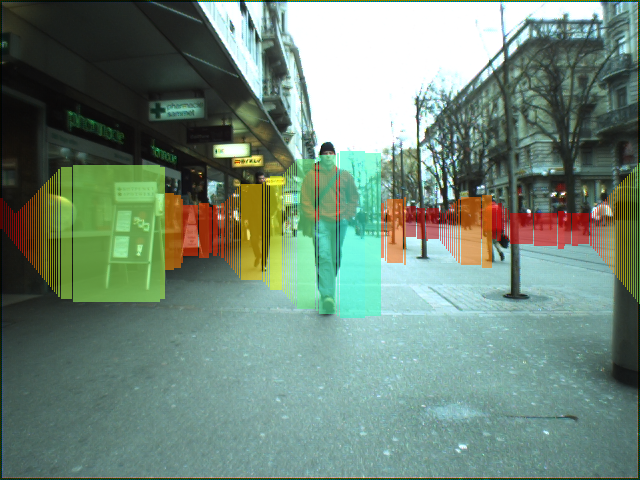
\includegraphics{stixels_over_original}
  \caption{Stixels superimposed to the frame from which they were extracted.}\label{fig:cp04_stixels}
\end{figure}

\subsection{Tracking}\label{ch:chapter04_01_03}

At this point, we are ready to start tracking the stixels. As said before this tracking has been performed using two different approaches: one consists on two different tracking levels from the first one tracks the stixels independently (that is, each stixel at the previous frame $t - 1$ is matched with another - or none - at the current frame $t$). So it becomes a matching problem in which we try to find the minimal cost matching between frames. In \cite{gunyel2012stixels}, this minimal matching was done using \ac{DP}. In our implementation we use a bipartite graph matching based method. In a second level, stixels are clustered into objects, which are matched based on the previous stixels tracking.

In the other approach, just the second level is performed, tracking obstacles based on one of the cost metrics, without considering the stixels included in the objects (except for the clustering process). In the next sections, the tracking process is described. Please note that the process described in section \ref{ch:chapter04_01_03_01} is performed only for the two-level approach, while the process in \label{ch:chapter04_01_04} is common to both approaches, except from the differences explicitly indicated in that section.

For this stage, we made some assumptions:
\begin{itemize}
 \item First, we assume that all stixels have been properly estimated.
 \item The maximal speed of the objects is limited, so we limit the search range between stixels to a certain threshold. This range depends on the distance of the stixel at the current frame and the frame rate. As there is just one stixel per column, we can limit also the matching process to a search into the $u$ direction.
 \item There is not a big temporal difference between two consecutive frames. That means that the same stixel at time $t$ and $t - 1$ should be similar. Also their height in meters should be similar. \notsure{As shown in section \ref{ch:chapter04_02_03_02}, this temporary consistence is more or less restrictive depending on the approach finally used for the tracking process.}
\end{itemize}

\subsubsection{Stixels-level tracking}\label{ch:chapter04_01_03_01}

In this stage, the tracking is performed at stixel level. As we just try to match each stixel at column $q_i\{t\}$ with another in the previous frame $t - 1$, we can think on this process as a matching problem. The way in which we have solved this is through a bipartite graph, in which nodes are the stixels at frame $t$ and $t - 1$, and the edges are associated to a certain movement cost $c_m$, which is represented by the equation:

\begin{equation}\label{eq:cp04_stixel_movement_cost}
  c_m(u_i\{t\}, u_j\{t - 1\}) = 
  \begin{align*}
    \begin{cases}
    f_{cost}(u_i\{t\}, u_j\{t - 1\}) & \textbf{if} \text{ matching is applicable} \\
    \infty & \textbf{otherwise}
    \end{cases}
  \end{align*}
\end{equation}

Here, a matching is applicable if and only if the following restrictions are satisfied:
\begin{itemize}
 \item $|X(u_i\{t\}) - X(u_j\{t - 1\})| < \tau_{max\_disp}$, where the free parameter $\tau_{max\_disp}$ indicates the maximal displacement of a certain stixel between frames; and $X(u)$ refers to its $X$ position in 3d coordinates.
 \item $u_i\{t\}$ is not a new stixel. That is, this is not the very first frame in which the stixel appears.
 \item Stixels $u_i\{t\}$ and $u_j\{t - 1\}$ are not occluded.
 \item $f_{cost}(u_i\{t\}, u_j\{t - 1\}) < \tau_{max\_cost}$.
\end{itemize}

Else, the cost is considered as infinity, so the link is not included in the graph. $f_{cost}(u_i\{t\}, u_j\{t - 1\})$ is a cost function which can be composed by different cost metrics, weighted by a set of parameters in the form:

\begin{equation}\label{eq:cp04_cost_function}
\small
  \begin{align*}
  f_{cost}(u_i\{t\}, u_j\{t - 1\}) =~  & & \alpha_{SAD} & ~\cdot~ & f_{SAD}(u_i\{t\}, u_j\{t - 1\}) \\
      & + & \alpha_{hist} & ~\cdot~ & f_{hist}(u_i\{t\}, u_j\{t - 1\}) \\
      & + & \alpha_{height} & ~\cdot~ & f_{height}(u_i\{t\}, u_j\{t - 1\})
  \end{align*}
\end{equation}

Here, $\alpha_{SAD} + \alpha_{hist} + \alpha_{height} = 1$. $f_{SAD}(u_i\{t\}, u_j\{t - 1\})$, $f_{hist}(u_i\{t\}, u_j\{t - 1\})$ and $f_{height}(u_i\{t\}, u_j\{t - 1\})$ are the factors for the different cost metrics being tested, which are described next.

\subsubsection{\acf{SAD}}\label{ch:chapter04_01_03_01_01}

This cost is computed as the pixel-wise sum of the absolute differences over the RGB color scheme between $u_i\{t\}$ and $u_j\{t - 1\}$, following the expression

\begin{equation}\label{eq:cp04_stixel_movement_sad_cost}
\tiny
f_{SAD}(u_i\{t\}, u_j\{t - 1\}) = 
\overset{v_b(q_i\{t\})}{\underset{v_1=v_a(q_i\{t\})}{\sum}}
\overset{v_b(q_j\{t - 1\})}{\underset{v_2=v_a(q_i\{t - 1\})}{\sum}}
| I_L\{t\}(u_i\{t\}, v_1) - I_L\{t - 1\}(u_j\{t - 1\}, v_2) |
\end{equation}

As it is very unlikely for both stixels to have the exact same height, they are resized to a dimension of $30\,px$. This metric was originally used in \cite{gunyel2012stixels} for the computation of the movement of the stixels. It has been used in our tests to compare the our results with those obtained by them in their implementation.

\subsubsection{Histograms matching}\label{ch:chapter04_01_03_01_02}

As said, the same stixel has not always the same size in different frames. This can happen because the position of the object partially represented by the stixel can change its depth in the scene, or due to noise in the height detection of the stixel. In order to normalize this, we have computed the histogram of each of the stixels being compared. Then, the cost is computed from the Hellinger distance between both histograms:

\begin{equation}\label{eq:cp04_stixel_movement_histograms_cost}
f_{SAD}(u_i\{t\}, u_j\{t - 1\}) = 2 \cdot \sqrt { 1 - \underset{i=1}{\overset{d}{\sum}}\sqrt{H(u_i\{t\})[i] \cdot H(u_j\{t - 1\})[i]}}
\end{equation}

Here, $H(u)[i]$ is the $i^{th}$ bin of the histogram computed for the stixel $u$, and $d$ is the number of bins in the histogram. In our implementation, $d = 256$.

\subsubsection{Height difference}\label{ch:chapter04_01_03_01_05}

This metric is used to complement the other two metrics, as by its own is not enough to do a matching, but it is good enough to help in the decision, in case of very similar scores in two or more possible matches. $f_{height}$ is computed as follows:

\begin{equation}\label{eq:cp04_stixel_movement_height_cost}
f_{height}(u_i\{t\}, u_j\{t - 1\}) = 1 - |h(u_i\{t\} - h(u_j\{t - 1\})|
\end{equation}

, where $h(u)$ is the height of the stixel in column $u$. 

In our tests, we have tried different values for $\alpha_{SAD}$, $\alpha_{hist}$ and $\alpha_{height}$, obtaining the results shown in section \ref{ch:chapter04_02}, both in terms of performance and time. As said, the value obtained using the function $f_{cost}$ is used to weight the links between the nodes of a bipartite graph. This graph, whose nodes are the stixels at times $t$ and $t - 1$, is shown at figure \ref{fig:cp04_bipartite_graph}. In the top row, we can see the nodes (stixels) at current time, while in the lower row, previous stixels are represented. Costs of the match are represented by the edges, depicted in the image with the notation $\omega_{i,j}$.

\begin{figure}[h!]
\centering
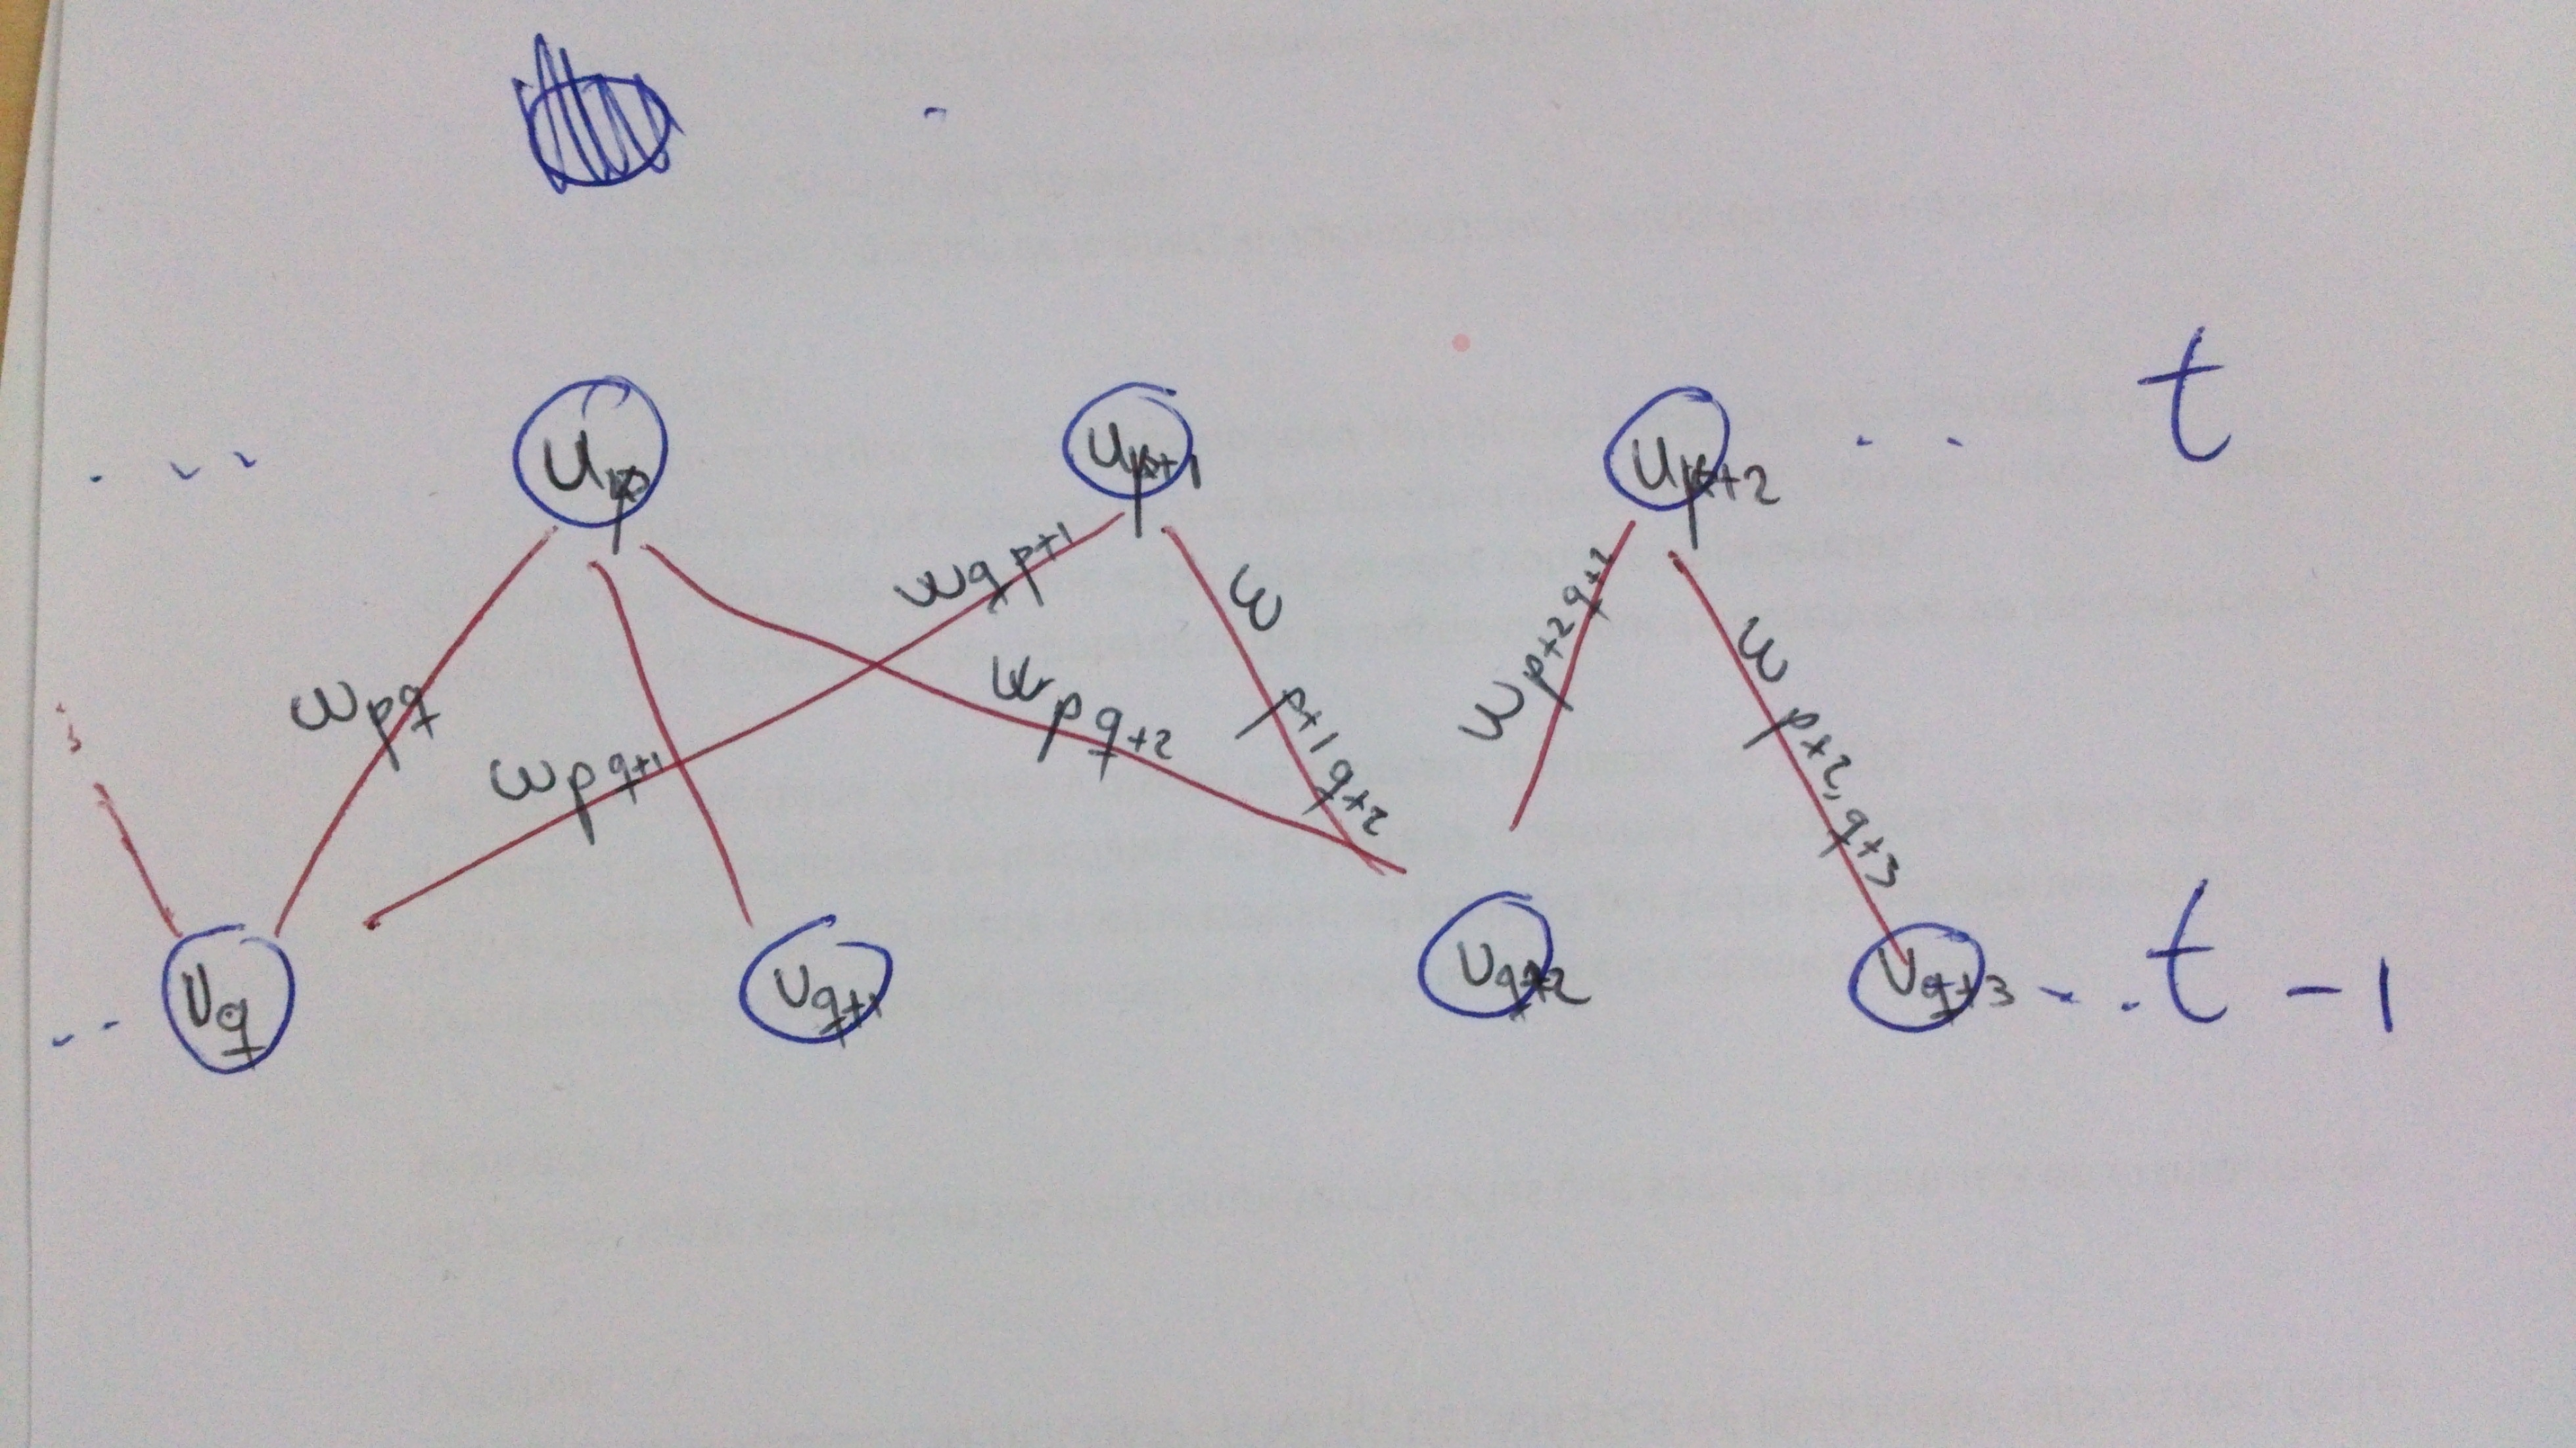
\includegraphics{bipartite_graph}
\caption{Representation of the bipartite graph used for the matching process.}\label{fig:cp04_bipartite_graph}
\end{figure}

Over this graph, we solve the following minimization problem:

\comment{No estoy seguro de esta notación}
\begin{equation}\label{eq:cp04_match_minimization}
\mathcal{\hat{M}}=\underset{\mathcal{M}}{\arg\min} \underset{(i, j) \in \mathcal{M}}{\sum} \omega_{i,j}, 
~~~~\exists! (i, \cdot) \wedge \exists! (\cdot, j)
\end{equation}

This problem is solved using a $O(n \cdot m \cdot log(n))$ implementation of the Edmond's maximum weighted matching algorithm (\cite{edmonds1965paths}). The advantages of using this method instead the \ac{DP} implementation by \cite{gunyel2012stixels} is that we getter better times that the implementation available and, specially, we can ensure that each match is performed one-to-one. That is, in the \cite{gunyel2012stixels} implementation, the same stixel could be matched with more than one stixel from the other frame. This is not good, as we can have multiple paths from the same stixel, so it is difficult to know the trajectory it has followed in the past. In our implementation, we choose the matching set that maximizes the whole matching, ensuring that one stixel is matched with \emph{only} one stixel in the other frame.

\subsection{Obstacle-level tracking}\label{ch:chapter04_01_04}

In this stage, we perform the tracking at obstacle level, and not at stixel level, as described in the previous section. In the case of two-level tracking, we should have at this point the set of matchings $m(i,j) \in \mathcal{M}$, which relates each stixel at column $u_i$ in the frame $t$ with the stixel at column $u_j$ in the frame $t - 1$. Anyway, we do not really need to have these matches for this stage, and do the tracking directly at the obstacle level. This section comprises two steps: object detection (clustering) and object tracking.

\subsubsection{Clustering}\label{ch:chapter04_01_04_01}

From left to right, stixels are being evaluated using the algorithm shown at algorithm \ref{alg:cp04_clustering}.

\begin{algorithm}
\caption{Clustering algorithm}
\label{alg:cp04_clustering}
\begin{algorithmic}
\Function{Clustering}{$\mathcal{Q}\{t\}$}
  \State {$\mathcal{O} \gets \emptyset$}
  \State {$o \gets \emptyset$}
  \For {\textbf{each} stixel $q_i \in \mathcal{Q}$, from left to right}
    \If {$|depth(q_i) - depth(q_{i-1})| > \tau_{depth\_dist}$}
      \If {$|depth(q_i) - depth(q_{i-1})| > \tau_{depth\_dist}$}
	\State {$width(o) > \tau_{min\_width}$}
      \EndIf
      \State {$o \gets \emptyset$}
    \EndIf
    \State {$o \gets o \cup q_i$}
  \EndFor
\EndFunction
\end{algorithmic}
\end{algorithm}

There, $\mathcal{Q}\{t\}$ is the set of stixels for the current frame $t$. From left to right, we start accumulating stixels, until the difference in depth between a certain pair of stixels is above a threshold $\tau_{depth\_dist}$, which is a user-defined free parameter. When this difference appears, we consider that we reached the right border of the obstacle, so it is added to the set $\mathcal{O}$, and a new obstacle is started. In case an obstacle is not wide enough, this obstacle is rejected. The reason for that is there are a stixel for each column, so there is a lot of noise that must be removed. This effect is easy to notice if we look at figure \ref{fig:cp04_stixels}.

At the end of the process, we will have got the set of obstacles $o_i \in \mathcal{O}$. Each obstacle has associated several parameters. One of them is the depth, which is computed as the minimal depth of all the associated stixels. In the left image of figure \ref{fig:cp04_clustering_aggregation}, the output obtained once this process has finished is shown.

\paragraph{Obstacle aggregation}\label{ch:chapter04_01_04_01_01}

In certain cases, due to a bad stixel detection, some stixels are located wrongly at a different depth from their real position. This effect happens, for example in cases like that shown at the left image of figure \ref{fig:cp04_clustering_aggregation}, in which a person in a fist plane opens his legs wide enough to show a big portion of the ground which is after him. This confuses the stixels detection algorithm, which thinks that the base of the obstacle is the central part of this person, and not his feet.

To solve this problem, the process described in algorithm \ref{alg:cp04_aggregation} is performed.

\begin{algorithm}
\caption{Aggregation algorithm}
\label{alg:cp04_aggregation}
\begin{algorithmic}
\Function{Aggregation}{$\mathcal{O}$}
  \State {$\mathcal{O'} \gets \emptyset$}
  \State {$o' \gets \emptyset$}
  \For {\textbf{each} object $o_i \in \mathcal{O}$, from left to right}
    \If {$|X(o_i) - X(o_{i-1})| > \tau_{lateral\_aggregation\_dist}$ \textbf{or}\\ \indent\indent\indent
	 $|Z(o_i) - Z(o_{i-1})| > \tau_{depth\_dist}$ \indent\indent~}

      \State {$\mathcal{O} \gets \mathcal{O} \cup o'$}
      \State {$o' \gets \emptyset$}
    \EndIf
    \State {$o' \gets o' \cup o$}
  \EndFor
\EndFunction
\end{algorithmic}
\end{algorithm}

There, we test all obstacles previously detected, again from left to right. If the lateral distance (in world coordinates) is below a threshold $\tau_{lateral\_aggregation\_dist}$, we check again if the depth difference is below $\tau_{depth\_dist}$. If this condition is satisfied, both obstacles are joined together. In figure \ref{fig:cp04_clustering_aggregation}, an example of the output obtained from this process is shown. In the left image, the person in the first plane is divided into two different obstacles. After the aggregation process, this same person is assigned to a single obstacle. Depth of the obstacle is computed as the minimal depth of both original obstacles.

\begin{figure}[h!]
\begin{tabular}{cc}
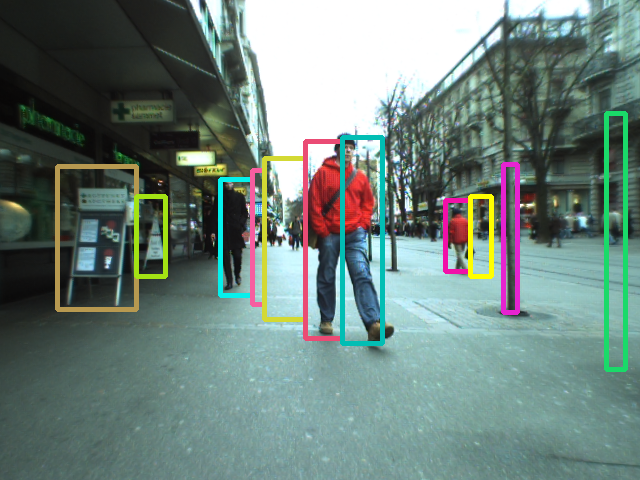
\includegraphics[width=0.49\textwidth]{obstaclesBeforeAggregation}\label{fig:cp04_before_aggregation} &
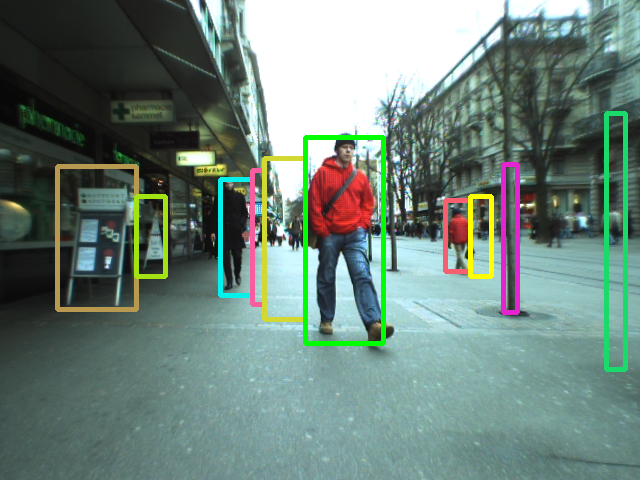
\includegraphics[width=0.49\textwidth]{obstaclesAggregated}\label{fig:cp04_after_aggregation}
\end{tabular}
\caption{Comparison of the obstacles detected before and after the aggregation process.}\label{fig:cp04_clustering_aggregation}
\end{figure}

\paragraph{Obstacle filtering}\label{ch:chapter04_01_04_01_02}

If we look again at figure \ref{fig:cp04_clustering_aggregation}, we will notice that we are still detecting some fake obstacles. For instance, between the man with the red jacket and that with the dark suit, there are two of them. Next to the man in the second plane, also with a red jacket, there is another fake obstacle, and there is a last one in the right side of the image. Signs and poles are not considered fake obstacles, as they are elements to avoid, and we do not have a classification scheme able to distinguish the class of the obstacle being detected.

In order to distinguish real obstacles from fake obstacles, we register the images obtained between frames, so we can distinguish the movement between frames. This movement can be originated both by the movement of the obstacle itself (i.e. a person walking), or by the movement of the camera respect to the obstacles. This makes occluded areas to appear, which allows detecting the border of obstacles that are not moving, but which we want to avoid. This is the case, for example, of the pole in the right part of the image.

The best way to do such a registration is through a polar rectification process, described at appendix \ref{ch:appendix_polar_calib}. With it, we will be able to align the current frame at time $t$ with another frame at time $t - k$. Using the aligned images, we get the pixel-wise absolute difference of both images, so we can get those pixels for which there is movement. This difference image is projected back to coordinates of the current image. Then, this difference is thresholded and binarized, rejecting the small differences produced by noise. Result of this process is shown at the top of figure \ref{fig:cp04_obstacle_filtering}. Then, for each obstacle, we get the associated \ac{ROI}. For each \ac{ROI}, we reject the top half of it, so we just look for movement in the area of the obstacle that is touching the ground. There are two reasons for that: the first one is that obstacles that move over the ground tend to have a higher movement in the lower part (for instance, legs or wheel movements). In the case of first plane static obstacles, the movement due to the camera change is more or less similar in the upper and lower half, so we are not loosing information. The second reason is that the stixels reconstruction assumes a planar ground in front of the camera, it is a fast way to discriminate bad correspondences.

\begin{figure}[h!]
  \begin{minipage}{\textwidth}
    \centering
    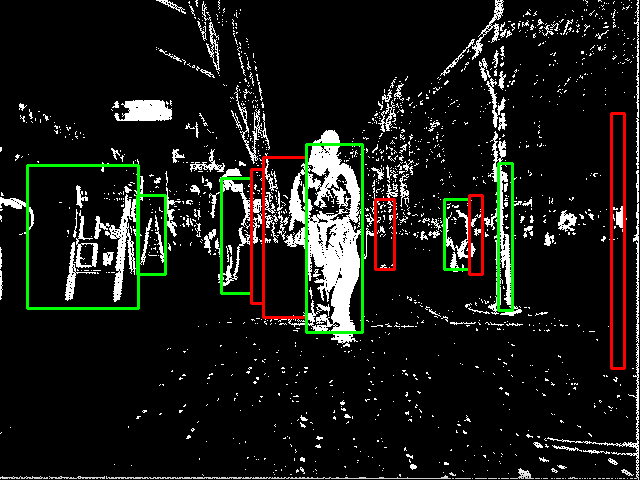
\includegraphics[width=\textwidth]{thresholdedPolar}
    \end{minipage}\hfill~
  \begin{minipage}{\textwidth}
    \centering
    \begin{tabular}{ |c|c|c|c|c|c|c|c|c|c|c|}
      \hline
      0 & 1 & 2 & 3 & 4 & 5 & 6 & 7 & 8 & 9 & 10 \\
      \hline
      
\includegraphics[width=0.15\textwidth, height=0.15\textwidth]{obstacleFilter/roi0} &
      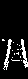
\includegraphics[width=0.15\textwidth, height=0.15\textwidth]{obstacleFilter/roi1} &
      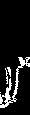
\includegraphics[width=0.15\textwidth, height=0.15\textwidth]{obstacleFilter/roi2} &
      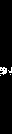
\includegraphics[width=0.15\textwidth, height=0.15\textwidth]{obstacleFilter/roi3} &
      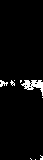
\includegraphics[width=0.15\textwidth, height=0.15\textwidth]{obstacleFilter/roi4} & 
      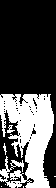
\includegraphics[width=0.15\textwidth, height=0.15\textwidth]{obstacleFilter/roi5} &
      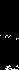
\includegraphics[width=0.15\textwidth, height=0.15\textwidth]{obstacleFilter/roi6} &
      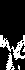
\includegraphics[width=0.15\textwidth, height=0.15\textwidth]{obstacleFilter/roi7} &
      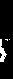
\includegraphics[width=0.15\textwidth, height=0.15\textwidth]{obstacleFilter/roi8} &
      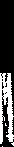
\includegraphics[width=0.15\textwidth, height=0.15\textwidth]{obstacleFilter/roi9} &
      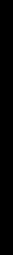
\includegraphics[width=0.15\textwidth, height=0.15\textwidth]{obstacleFilter/roi10} \\
      \hline
      \setlength{\fboxsep}{1pt}\fcolorbox{green}{green}{\includegraphics[width=0.15\textwidth, height=0.15\textwidth]{obstacleFilter/occ0}} &
      \setlength{\fboxsep}{1pt}\fcolorbox{green}{green}{\includegraphics[width=0.15\textwidth, height=0.15\textwidth]{obstacleFilter/occ1}} &
      \setlength{\fboxsep}{1pt}\fcolorbox{green}{green}{\includegraphics[width=0.15\textwidth, height=0.15\textwidth]{obstacleFilter/occ2}} &
      \setlength{\fboxsep}{1pt}\fcolorbox{red}{red}{\includegraphics[width=0.15\textwidth, height=0.15\textwidth]{obstacleFilter/occ3}} &
      \setlength{\fboxsep}{1pt}\fcolorbox{red}{red}{\includegraphics[width=0.15\textwidth, height=0.15\textwidth]{obstacleFilter/occ4}} & 
      \setlength{\fboxsep}{1pt}\fcolorbox{green}{green}{\includegraphics[width=0.15\textwidth, height=0.15\textwidth]{obstacleFilter/occ5}} &
      \setlength{\fboxsep}{1pt}\fcolorbox{red}{red}{\includegraphics[width=0.15\textwidth, height=0.15\textwidth]{obstacleFilter/occ6}} &
      \setlength{\fboxsep}{1pt}\fcolorbox{green}{green}{\includegraphics[width=0.15\textwidth, height=0.15\textwidth]{obstacleFilter/occ7}} &
      \setlength{\fboxsep}{1pt}\fcolorbox{red}{red}{\includegraphics[width=0.15\textwidth, height=0.15\textwidth]{obstacleFilter/occ8}} &
      \setlength{\fboxsep}{1pt}\fcolorbox{green}{green}{\includegraphics[width=0.15\textwidth, height=0.15\textwidth]{obstacleFilter/occ9}} &
      \setlength{\fboxsep}{1pt}\fcolorbox{red}{red}{\includegraphics[width=0.15\textwidth, height=0.15\textwidth]{obstacleFilter/occ10}} \\
      \hline
    \end{tabular}
  \end{minipage}\hfill
  \caption{Object filtering process. In the top, the binarized motion image is shown ($k=0.2$). In the bottom, the occupancy maps generated for each candidate obstacle.}\label{fig:cp04_obstacle_filtering}
\end{figure}

Each region is transformed to real world coordinates and project there the points resulting after the thresholding process. There, the region is dividided in cells (in our tests, of $10\times10\,cm$). For each cell, if there is at least one point falling inside it in the plane $XY$, the cell is marked as occupied. The occupancy grids obtained, together with their associated \ac{ROI} in the motion image, are shown in the table in figure \ref{fig:cp04_obstacle_filtering}. \acs{ROI} are in the first row, and occupancy maps in the second. It is easy to see that real obstacles, like for example number 5 or number 7, present a higher density if compared with, for example, the obstacle number 4. Also, if we look at obstacle 2, a man in a black suit (which makes the motion detection a little bit more complicated through absolute differencing due to the low color values), is properly detected. In order to ensure the detection of this kind of obstacles, it is important to choose a value for $k$ big enough. In our tests, we decided to use $k = 0.2\,s$, so we are sure that differences are appreciable, but being conservative at the same time. At the end of the process, we decide if the obstacle is rejected or not through the following equation:

\begin{equation}\label{eq:cp04_fake_obstacles}
  fake(o) = 
  \begin{align*}
    \begin{cases}
      true & \text{if } {{count(G_o, true)} \over {count(G_o, true) + count(G_o, false)}} > \tau_{occ} \\
      false & otherwise
    \end{cases}
  \end{align*}
\end{equation}

There, $count(G_o, j)$ counts the number of occupied ($j=true$) or free ($j=false$) cells in the occupancy grid corresponding to the object $o$, $G_o$. $\tau_{occ}$ is a parameter. We also check that the width of each obstacle in real world coordinates is inside the limits. We can see the results obtained for this process again in figure \ref{fig:cp04_obstacle_filtering}. Rejected obstacles are highlighted in red, while the accepted are represented in green.

\subsubsection{Tracking}\label{ch:chapter04_01_04_02}

Once we have the obstacles detected and filtered, we propose two approaches for the object tracking. The first one takes advantage of the process described in section \ref{ch:chapter04_01_03_01}. From the initial matching performed at stixel level, we try to maximize the number of matches between obstacles. The second one tries to do the matching directly. As there is not a big difference between frames, we can use template matching techniques in order to do the tracking. As we will see in section \ref{ch:chapter04_02_03}, each of these techniques has its own advantages. The first one presents a better recall along the frames; however, the second is faster, with a recall that, despite of being not as good as that for the two-level tracking scheme, is still good.

\paragraph{Two-level tracking case}\label{ch:chapter04_01_04_02_01}

As said, the two-level tracking takes advantage from the stixels matched using the method in \ref{ch:chapter04_01_03_01}, together with the obstacles found using the method described in the last section. Again, we consider the tracking problem as a pair matching process that is repeated along the time. Based on that idea, we define the correspondence matrix $C_{|\mathcal{O}\{t\}| \times |\mathcal{O}\{t - 1\}|}$, which counts the number of correspondences obtained at stixel level between the stixels at the current frame and the previous one. This process is described in the algorithm \ref{alg:cp04_two_level_tracking}.

\begin{algorithm}
\caption{Two-level tracking algorithm}
\label{alg:cp04_two_level_tracking}
\begin{algorithmic}
\Function{Tracking}{$\mathcal{O}\{t\}$, $\mathcal{O}\{t - 1\}$}
  \State {$C_{|\mathcal{O}\{t\}| \times |\mathcal{O}\{t - 1\}|} \gets 0$}
  \For {\textbf{each} object $o\{t\} \in \mathcal{O}\{t\}$}
    \For {\textbf{each} stixel $q\{t\} \in o$}
      \State {Find correspondence $q\{t - 1\}$ for $q\{t\}$}
      \State {Find the object $o\{t - 1\} \in \mathcal{O}\{t - 1\}$ associated to $q\{t - 1\}$}
      \If {$o\{t - 1\}$ found \textbf{and} $\|o\{t\} - o\{t - 1\}\| < \tau_{max\_obst\_dist}$}
	\State {$C(o\{t\}, o\{t - 1\}) \gets C(o\{t\}, o\{t - 1\}) + 1$}
      \EndIf
    \EndFor
  \EndFor
\EndFunction
\end{algorithmic}
\end{algorithm}

Two objects can be associated between frames if there is at least one stixel correspondence and they are close enough, as we assume the movement between frames should not be too big as the frame rate is high enough. With this cost matrix, we solve the following maximization problem:

\begin{equation}\label{eq:cp04_two_level_maximization}
\mathcal{\hat{C}}=\underset{\mathcal{C}}{\arg\max} \underset{(i, j) \in \mathcal{M}}{\sum} C(i,j),
~~~~\exists! (i, \cdot) \wedge \exists! (\cdot, j)
\end{equation}

After this process, we will have the set of pairs $\mathcal{\hat{C}}$. In our implementation, we maintain an internal structure that associates each track to each obstacle in the last tracked frame. These tracks are extended in order to include the new objects, which will be used as the new indexes of the trajectories list. In figure \ref{fig:cp04_tracking_examples_two_level}, we can see several examples of the results obtained using this tracking method. For more information about the performance obtained, please check the results in section \ref{ch:chapter04_02} \notsure{, or check the videos available at XXX}.

\begin{figure}[h!]
    \centering
    \begin{tabular}{ ccccc}
      \includegraphics[width=0.45\textwidth]{sequenceTwoLevel/twolevel30}\label{fig:cp04_two_level_example_15} &
      \includegraphics[width=0.45\textwidth]{sequenceTwoLevel/twolevel320}\label{fig:cp04_two_level_example_126} &
    \end{tabular}
  \caption{Some tracking results using the two-level based tracking.}\label{fig:cp04_tracking_examples_two_level}
\end{figure}

\paragraph{Object tracking case}\label{ch:chapter04_01_04_02_02}

The object tracking scheme is quite similar. However, in this case the cost matrix is not generated by counting the number of stixels associated to each obstacle, as we do not have this information (remember that for this approach, we do not apply the process described in section \ref{ch:chapter04_01_03_01}). Instead of that, we use the histograms difference for each pair of obstacles, in a process similar to that described in section \ref{ch:chapter04_01_03_01_02}, so the cost matrix in this case is defined as:

\begin{equation}\label{eq:cp04_object_matching_histograms_cost}
C(o\{t\}, o\{t - 1\}) = 1 - \left ( 2 \cdot \sqrt { 1 - \underset{i=1}{\overset{d}{\sum}}\sqrt{H(o\{t\})[i] \cdot H(o\{t - 1\})[i]}} \right )
\end{equation}

Then, the tracking problem is the same as explained for the two-level tracking case: we solve the maximization problem defined in \ref{eq:cp04_two_level_maximization}, and then the tracks are updated with the results of the matching. In figure \ref{fig:cp04_tracking_examples_object}, some other examples of the output obtained after applying this process are shown.

\begin{figure}[h!]
    \centering
    \begin{tabular}{ccccc}
      \includegraphics[width=0.45\textwidth]{sequenceObstacle/obstacle15}\label{fig:cp04_object_level_example_30} &
      \includegraphics[width=0.45\textwidth]{sequenceObstacle/obstacle126}\label{fig:cp04_object_level_example_320}
    \end{tabular}
  \caption{Some tracking results using the object based tracking.}\label{fig:cp04_tracking_examples_object}
\end{figure}

\section{Results}\label{ch:chapter04_02}

In this section, we will show some evaluation results obtained after the evaluation of the method described in this chapter. Evaluations have been focused into four different scopes: 

\begin{itemize}
 \item Quality of the clustering process.
 \item Accuracy of the depth obtained for the computed stixels compared to object level results.
 \item Recall of the obtained tracks related to several conditions.
 \item Computation time.
\end{itemize}

In order to compare our results with those obtained by \cite{gunyel2012stixels} and \cite{benenson2011stixels}, we have used the \emph{Bahnhof} sequence (\cite{ess2009robust}), which contains about 7400 obstacle annotations with height $\geq 40\,px$ on 999 stereo pairs, with an image resolution of $640 \times 480$ pixels and a frame rate of about 15 frames per second. All tests described in this section have been performed over this sequence.

\subsection{Clustering}\label{ch:chapter04_02_01}

In this test, we want to know if the obstacle detection method described in section \ref{ch:chapter04_01_04_01} is good enough. For that, we compared our detections with the real obstacles appearing in each current frame. In these tests, we have executed the method with and without performing the filtering process described in section \ref{ch:chapter04_01_04_01_02}, obtaining the results shown in figure \ref{fig:cp04_detection_rate}.

\begin{figure}[h!]
\centering
\includegraphics[trim=50 40 80 60,clip]{detectionRate}
\caption{Obstacles detection rate achieved using our clustering method.}\label{fig:cp04_detection_rate}
\end{figure}

There, we compare each recall value with the number of frames in the sequence falling below it. That is, the faster the plot grows, the better the results are. There, we can see that, for a recall value of 90\%, just a 40\% fall below this value for the case in which we are filtering the obstacles. Situation is different when objects are not filtered. For the same recall value, a 60\% of the frames in the sequence are below this value.

In figure \ref{fig:cp04_clustering_comparison}, we can see the projected 3d output of the detected stixels. In the left image, the original stixels are shown. As we can see, there is a lot of noise, specially between obstacles. We can see also that a lot of free areas are detected. In the right image we show just the stixels falling inside an obstacle, and with their depths restored.

\begin{figure}[h!]
\begin{tabular}{cc}
\includegraphics[width=0.49\textwidth]{stixelsDetection}\label{fig:cp04_stixels_detection} &
\includegraphics[width=0.49\textwidth]{obstacleDetection}\label{fig:cp04_obstacle_detection}
\end{tabular}
\caption{Comparison of the stixels obtained trough the method of \cite{benenson2012pedestrian} and the clustering performed in our method.}\label{fig:cp04_clustering_comparison}
\end{figure}

\subsection{Stixel accuracy}\label{ch:chapter04_02_02}

In this section, we want to show the accuracy found in the depth computation for the stixels regarding to our reconstruction based just on the obstacles. There, we compare the disparity error regarding to a \ac{ELAS} reconstructed disparity map wit the percentage of frames below this error. The red line represents the stixels error, which grows faster than the error shown by the clustered obstacles. If we look at the $x-coordinates$, we can see that approximately a 95\% of the images have a disparity error below a 10\%, while this error is just found for a 60\% of the images when the reconstruction is made buy just the original stixel computation.

\begin{figure}[h!]
\centering
\includegraphics[trim=50 40 80 60,clip]{disparity}
\caption{Difference in disparity achieved for both our clustering method and the initial stixel reconstruction.}\label{fig:cp04_disparity_comparison}
\end{figure}

In figure \ref{fig:cp04_reconstruction}, we show the disparity maps presented by \ac{ELAS}, the original stixels from \cite{benenson2011stixels} and our clustered obstacles. These are represented by a color scale, which is shown in the right side of the images. In this scale, the lower disparities (further) are represented in red, while the highest disparities are represented in blue.

\begin{figure*}[h!]
        \centering
        \begin{subfigure}[b]{0.25\textwidth}
	  \begin{tabular}{c}
	    \includegraphics[width=\textwidth]{elas}
	  \end{tabular}
	  \caption{ELAS.}\label{fig:cp04_reconstruction_elas}
        \end{subfigure}% 
        ~
        \begin{subfigure}[b]{0.25\textwidth}
	  \begin{tabular}{c}
	    \includegraphics[width=\textwidth]{stixels}
	  \end{tabular}
	  \caption{Stixels.}\label{fig:cp04_reconstruction_stixels}
        \end{subfigure}%       
        ~
        \begin{subfigure}[b]{0.25\textwidth}
	  \begin{tabular}{c}
	    \includegraphics[width=\textwidth]{objects}
	  \end{tabular}
	  \caption{Object clustering.}\label{fig:cp04_reconstruction_objects}
        \end{subfigure}%    
        ~
        \begin{subfigure}[b]{0.25\textwidth}
	  \centering
	  \begin{tabular}{c}
	    \includegraphics[height=0.375\figuresheight]{colorscale_jet}
	  \end{tabular}
	  \caption*{}\label{fig:cp04_reconstruction_colorscale}
        \end{subfigure}% 
        \caption{Comparison of the disparities obtained for \ac{ELAS}, stixels and the reconstructed objects.}\label{fig:cp04_reconstruction}
\end{figure*}

\subsection{Tracking}\label{ch:chapter04_02_03}

In this section, the results obtained in our tracking evaluation tests are shown in terms of the recall measured related to two different criteria: the behavior of the tracking after a few frames (that is, the track length achievable with a certain level of confidence); and the behavior when the time between frames is increased. 

In our tests, we have tried with different configurations attending to the matching metrics and the method used. From the whole set of tests, we have selected the most representative, which are shown in table \ref{table:cp04_configurations_tested}.

\begin{table}[h]
\begin{center}
\begin{tabular}{|c|c|c|c|c|}
  \hline
 \multirow{2}{*}{Name} & \multicolumn{3}{ c| }{Cost factors} & \multirow{2}{*}{Tracking Method} \\ \cline{2-4}
 & $\alpha_{SAD}$ & $\alpha_{hist}$ & $\alpha_{height}$ &  \\
 \hline
 Conf. 1 & 1 & 0 & 0 & \cite{gunyel2012stixels} \\
 Conf. 2 & 0.5 & 0 & 0.5 & \cite{gunyel2012stixels} \\
 \hline
 Conf. 3 & 1 & 0 & 0 & Two-level tracking \\
 Conf. 4 & 0.5 & 0 & 0.5 & Two-level tracking \\
 Conf. 5 & 0 & 1 & 0 & Two-level tracking \\
 Conf. 6 & 0 & 0.5 & 0.5 & Two-level tracking \\
 \hline
 Conf. 7 & 0 & 0 & 0 & Object tracking \\
 \hline
\end{tabular}
\end{center}
\caption{Configurations for which the evaluation results are shown.}\label{table:cp04_configurations_tested}
\end{table}

Two of these configurations are from the implementation of the method by \cite{gunyel2012stixels}, available at \url{https://bitbucket.org/rodrigob/doppia}, with just the \ac{SAD} cost, and the final configuration described in their paper, in which $\alpha_{SAD} = 0.5$ and $\alpha_{height} = 0.5$, in order to know the real contribution of factor $\alpha_{height}$. Same process is done for the two-level tracking method, in which we evaluate also the contribution of factor $\alpha_{hist}$. Finally, we do a evaluation of the results obtained by using the object based tracking, without doing a previous stixel level tracking. As this level is not needed, $\alpha_{SAD} = \alpha_{hist} = \alpha_{height} = 0$.

\subsubsection{Performance along the sequence}\label{ch:chapter04_02_03_01}

For the evaluation of the tracking capabilities of the method, we followed the same strategy as \cite{gunyel2012stixels}: we used annotated obstacle bounding boxes provided as ground truth with the evaluated sequence. Starting from ground truth annotations at a certain frame, each evaluated configuration is used to predict the bounding box positions up to $\Delta$ frames in the future. For each frame, we evaluate the recall using the standard intersection over union metric. By running this evaluation starting from every frame in a video sequence we obtain the \emph{recall vs. $\Delta$ frames} curve shown at figure \ref{fig:cp04_recall_vs_delta_frames}, that can be used to compare the configurations. 

\begin{figure}[h!]
\centering
\includegraphics[trim=50 40 80 60,clip]{recall_vs_delta_frames}
\caption{Comparison of the recall obtained for the different configurations.}\label{fig:cp04_recall_vs_delta_frames}
\end{figure}

In this chart, we can see that the \cite{gunyel2012stixels} method falls quite fast, with a recall below 50\% just after 5 frames have passed. Also, we notice that the contribution of $\alpha_{height}$ is not clear. About the two-level tracking methods, results are better, specially those in which $\alpha_{hist} \neq 0$. There are many reasons for that. Respect with the method of \cite{gunyel2012stixels}, the use of obstacles for the tracking instead of just the stixels filters a lot of noise, making the tracking more reliable. This is confirmed if we look at figure \ref{fig:cp04_tracking_examples}, where we can see the tracking performed by \emph{Configuration 1}, \emph{Configuration 5} and \emph{Configuration 7}. If we look at the first two images, we can see that the trajectories obtained for the \emph{Configuration 5} are longer, and smoother. About the difference between using $\alpha_{hist}$ or $\alpha_{SAD}$, the histograms being used are normalized just before the matching, while the sum of absolute differences is done pixel by pixel, without considering illumination changes.

Finally, object based tracking shows good results for the first frames, but it falls a little bit faster than the two-level based tracking methods. We think the most likely reason for that is that the two-level tracking is more tolerant to the clustering errors. For example, if in one frame we consider as part of the obstacle a relatively big fraction of the background, the aspect of the histogram will change, so the matching score could be small. Looking again at figure \ref{fig:cp04_tracking_examples}, we can see that the quality of the tracks both in configurations 5 and 7 is comparable, but the length of the former is bigger.

\begin{figure*}[h!]
        \centering
        \begin{subfigure}[b]{0.33\textwidth}
	  \begin{tabular}{c}
	    \includegraphics[width=\textwidth]{trackingConf1}
	  \end{tabular}
	  \caption{Conf. 1.}\label{fig:cp04_tracking_example_conf_1}
        \end{subfigure}% 
        ~
        \begin{subfigure}[b]{0.33\textwidth}
	  \begin{tabular}{c}
	    \includegraphics[width=\textwidth]{trackingConf5}
	  \end{tabular}
	  \caption{Conf. 5.}\label{fig:cp04_tracking_example_conf_5}
        \end{subfigure}%       
        ~
        \begin{subfigure}[b]{0.33\textwidth}
	  \begin{tabular}{c}
	    \includegraphics[width=\textwidth]{trackingConf7}
	  \end{tabular}
	  \caption{Conf. 7.}\label{fig:cp04_tracking_example_conf_7}
        \end{subfigure}%
        \caption{Example of the tracking obtained for the different configurations, at stixel level.}\label{fig:cp04_tracking_examples}
\end{figure*}

\subsubsection{Performance at different frame increments}\label{ch:chapter04_02_03_02}

We also wanted to know which of the methods was more tolerant to low frame rate sequences, as one of the assumptions for the tracking methods is that the temporal difference between frames is not too big. Based on this, we evaluated the relation existing between the recall, $\Delta$ frames and the time step between frames. So we repeated the tests, but this time increasing $k$ frames each time, with $k=0.06\dots1.2\,s$ (Corresponding to 1 up to 20 frames at $15\,Hz$). Then, we evaluated the variation in the results. First, we did a few preliminary tests with just the first 200 frames in which we wanted to know the variation in the recall related to the time step. Results of this tests are represented in the chart shown at figure \ref{fig:cp04_recall_vs_step}. In this chart, we show the tracking values presented by the different configurations with just one frame increment at the time step shown in the $x$ axis. There, we can detect four different profiles, which are again related to the configurations 1-2, 3-4; 5-6, and 7. As before, we observe that the contribution offered by the $\alpha_{height}$ factor is negligible. We also observe that the most tolerant of all the configurations is number 7, as it was to be expected. This configuration does the tracking just at object level, so it is able to deal with changes slightly bigger than those with which the stixel level tracking is able to work properly. However, there is a surprise, as the tracking based in just the stixel level presents better values. The reason for that is that tracking using this method gets slightly better results in the first frames, but the recall falls faster along the frames.

\begin{figure}[h!]
\centering
\includegraphics[trim=50 40 80 60,clip]{recall_vs_step}
\caption{Behavior of the recall obtained for the different configurations at different frame increments.}\label{fig:cp04_recall_vs_step}
\end{figure}

This effect is better seen in figure \ref{fig:cp04_recall_vs_delta_frames_vs_step}, where we compare the three involved values (recall, $\Delta frames$ and $\Delta time$ for the configurations 1, 3, 5 and 7. There, we can see that when $\Delta frames \approx 0$, the pattern shown in the previous figure is repeated. However, when $\Delta frames$ starts growing we can see that configurations 3 and 5 do not fall as fast as configuration 1, which confirms the tests previously done. Configuration 7 remains higher with respect to the rest of configurations.

\begin{figure}[h!]
\centering
\includegraphics[trim=80 90 140 90,clip]{recall_vs_delta_frames_vs_step_28b_1_16b}
\caption{Comparison of the tracking capabilities at different frame increments for configurations \emph{Conf. 1}, \emph{Conf. 5} and \emph{Conf. 7}}\label{fig:cp04_recall_vs_delta_frames_vs_step}
\end{figure}

\subsection{Computation time}\label{ch:chapter04_02_04}

In figure \ref{fig:cp04_times_average}, we can see that, as expected, the faster of the methods is that for the \emph{Configuration 7}, as just object comparison is performed. This is quite faster, as just a few obstacles are compared per frame, against the 640 by 640 comparisons that can be achieved at stixel level in the worst case. From the rest, we see that the graph based methods are in average slightly faster than those based on dynamic programming. However, the time variance obtained when using the sum of absolute differences as measure is bigger. We do not have an explanation for that, probably if the situation is not quite discriminative, the graph based method needs more time for computing the matches.

\begin{figure}[h!]
\centering
\includegraphics[trim=50 40 80 60,clip]{times_average}
\caption{Times obtained for each configuration.}\label{fig:cp04_times_average}
\end{figure}

\section{Summary}\label{ch:chapter04_07}

In this chapter, we have seen a different solution for the object tracking for driver assistance applications, based on the stixel world by \cite{badino2009stixel}. Our work extends the work presented by \cite{gunyel2012stixels}, improving the results obtained by them. The use of a two-level based tracking gives robustness to the stixel tracking and is able to improve the reconstruction by joining stixels that were not in the same plane due to a bad reconstruction. We demonstrate that using the Hellinger distance between histograms give better results than the pure Sum of Absolute Differences, and that the use of the height as matching metric is negligible.
We also saw another tracking method in which the tracking is performed at obstacle level. In this case, results were not so good, but in certain applications can be useful due to a high performance time and a low decay in the recall when the frame rate is low.
In the future, we want to try to improve the way in which stixels are computed. We think that using the polar rectification for combining tracking and reconstruction could give good results. Also, the use of a measure of the goodness of the tracks at stixel level should help to improve the results obtained for the clustering process.
In the next chapter, we will see another obstacle tracking method in which 3D dense reconstruction is used as input.


% %%
%%  chapter05.tex - Obstacle Detection and Planning for Autonomous Vehicles based on Computer Vision Techniques
%%
%%  Copyright 2014 Néstor Morales <nestor@isaatc.ull.es>
%%
%%  This work is licensed under a Creative Commons Attribution 4.0 International License.
%%

\graphicspath{{./images/chapter05/bmps/}{./images/chapter05/vects/}{./images/chapter05/}}

\chapter{3D object tracking}\label{ch:chapter05}

As we have seen in previous chapters, we still have not solved completely the problem of detection and tracking of the obstacles. Image comparison could be, as said, a good input point for an obstacle classifier, but it is still not able to locate obstacles in the real world with respect to a map o to the vehicle. Also, it is not able to track the obstacles and it is very dependent on the goodness of the database of the area in which the vehicle is driving. Non-rigid point set registration method is not able to detect obstacles using moving cameras. \notsure{Stixels can be a solution, but they do not consider obstacles further from a first plane and they assume a flat road}. 

In this chapter, we will describe a method that, using a point cloud generated from a pair of moving stereo cameras, is able to detect obstacles and model them as a set of voxels. Also, it is able to decide the direction in which objects are moving to. The method described here is inspired in the work by \cite{danescu2012particle}, in the way that a particle filter is used over an occupancy grid in order to detect the obstacles and their directions. However, this method uses a two-dimensional grid. As said in section \ref{ch:chapter01_02_05}, methods based on such a grid are related to which we named as 2.5D methods. The main disadvantages of this kind of methods is that they consider all the obstacles as lying in the ground, and are represented as a convex cuboid that doesn't take into account the complexities of certain obstacles.
As commented in previous sections, Verdino is thought to work in crowded areas, like pedestrian streets or touristic complexes, in which an overestimation of the size of obstacles can lead to an inefficient behavior. So we decided to extend the original method of \cite{danescu2012particle} in order to make it fully three-dimensional, by using a voxelized grid instead of the original cartesian/polar grid, and including some improvements in order to reduce the number of fake positives, among others.

\section{The Method}\label{ch:chapter05_01}

In this method, we generate a voxelized occupancy grid in which the world surrounding the vehicle is divided into a discrete number of voxels of the same size. For each voxel, a occupancy probability is assigned based on the number of points inside the volume represented by it and its neighborhood. Also, during the process, a set of particles will be assigned dynamically during the execution, based on a 3D generalization of the weighting and resampling mechanism described in \cite{isard1998condensation}. These particles will have a double function:
\begin{enumerate}
 \item Denoting hypotheses (as happens with classical particle filters).
 \item Being the building blocks of our world model.
\end{enumerate}

Like this, at each frame, the set of particles obtained in the previous frame (each of these with a certain pose ${(x, y, z)}$ and speed ${(vx, vy, vz)}$) will be evolved using their movement model and assigned to the corresponding voxel, attending to the time that passed between frames and the ego-motion. Then, these particles are re-weighted and resampled.

At this point, particles that passed the resampling process are used to construct the objects that model the environment, joining all these voxels that share a similar orientation and speed. This object reconstruction is done by using a flood fill approach, in a way quite similar to that described in \cite{broggi2013}, but using the vectors of each voxel, instead of color information, as done in their work.

This particle-based approach inherits some advantages from the previous work by \cite{danescu2012particle}:
\begin{itemize}
 \item \emph{It is not necessary to estimate the probability distribution of the speed or the orientation.} These distributions, which in the past have been approximated as histograms (\cite{chen2006dynamic}), Gaussian mixtures (\cite{gindele2009bayesian}) or higher dimensions (\cite{coue2006bayesian}), are not required anymore due to the use the particles. This distribution is obtained directly from the surviving particles of each voxel. 
 \item \emph{Easy encoding of the past and present knowledge from sensor data.} The usage of a voxel grid makes this easier, and allows updating it dynamically when new information is available with a little computational cost.
\end{itemize}

Also, we add some new advantages in our approach:
\begin{itemize}
 \item \emph{Hierarchical object pose, orientation and speed detection.} Object units are detected at lower level as individual voxels, for which we know their individual speed and pose. Joining all these voxels together, we obtain the whole obstacle, whose pose and speed is directly dependent on the voxels which compose it. 
 \item \emph{Fully 3D perception of the object detected.} No previous assumption of the shape of the obstacles is taken, providing an accurate estimation of complex obstacles. The usage of voxels instead of cuboids, allows to have a clear idea of the actual shape of an obstacle, avoiding the overestimation of their real size, which is not acceptable for an application like that described in this Thesis. In this sense, we can have an accurate idea of 3D boundaries of an obstacle or reject it in case it is hanging, like in the case of traffic lights.
 \item \emph{No color information is used.} As we do not use color information coming from the input 3D point cloud, our implementation is ready to accept data from other sensors different from a stereo pair, like \ac{LIDAR}.
 \item \emph{Collaborative update of the grid.} The usage of a voxel grid also allows combining several input sources at the same time. We have not done any work in this sense, but our implementation is ready for such application.
\end{itemize}

The method pipeline is based on six different steps, depicted in figure \todo{ \ref{fig:cp05_pipeline_general} }:
\begin{enumerate}
 \item \emph{3D point cloud generation.} As said before, our implementation is able to work from data coming from any kind of sensor, but in this work, we have been working with stereo cameras. In this step we obtain, from a pair of calibrated images provided by a stereo pair of cameras, a set of 3D points that will be the actual input for our algorithm. At implementation level, this process is done in a separate process, so the point cloud can be used for other tasks in the system. More details of this process are given at section \todo{ \ref{chapter05_01_01} }.
 \item \emph{Ego-motion.} By using images, the orientation and speeds computed for the different objects is biased by the speed of the own vehicle. To avoid this, we need to know our own movement. In section \todo{ \ref{chapter05_01_02} }, this process is better explained.
 \item \emph{Voxelization.} Each of the 3D points obtained in the first step is assigned to a certain voxel. Each voxel has a certain resolution, which covers a parameterized section of the world. In our tests, we have used voxels of a resolution of $(0.25x0.25x0.25)$\,m in the $X$, $Y$ and $Z$ dimensions, respectively, covering a volume going from $-4$\,m to $+4$\,m in the $X$ axis; $0$ to $+24$\,m in the $Y$ axis; and $0$\,m to $3.5$\,m in the $Z$ axis. This process, and how probabilities are assigned to each voxel is explained at section \todo{\ref{chapter05_01_03}}.
 \item \emph{Voxel pose and speed computation.} Based on a \ac{PF} and in the probabilities assigned in the previous step, we calculate the pose and speed of each of the voxels in the grid, as explained in section \todo{\ref{chapter05_01_04}}.
 \item \emph{Object reconstruction.} Once we know the pose and speed of each voxel, and based on a flood fill procedure inspired in the work by \cite{broggi2013} and in the vectors already obtained, similar voxels are assigned to a common final obstacle. For each segmented object, orientation and speed is computed based on the vectors belonging to each of the associated voxels (See section \todo{\ref{chapter05_01_05}}).
 \item \emph{Planning and obstacle avoidance.} Once we know the exact position of the vehicles, and their future movement, we can integrate the results into the rest of the system and use it for the calculation of safe and smooth paths. This process will be described in more depth in the following chapters, in sections \todo{ \ref{chapter05_01_06} }.
\end{enumerate}

\begin{figure}[thb]\label{fig:cp05_pipeline_general}
  \centering
  \includegraphics{pipeline_general}
  \caption{Pipeline of the different steps of the method. \todo{Me olvidé de poner el módulo encargado de filtrar los puntos antes de la fase de voxelizado} }
\end{figure}

In the following sections, all these steps will be explained in a bigger detail.

\subsection{3D point cloud generation}\label{ch:chapter05_01_01}

In this stage, a pair of calibrated images is received and transformed into a disparity map, that will allow us to get the corresponding 3D point cloud. In \todoref{XXX}, we evaluated a set of algorithms, including some pre- and post-processing filters, in order to know which of these is the most suitable for outdoor autonomous navigation applications. From this evaluation, we concluded that best results were given by the configuration we named as \emph{Census-SGM Conf 2}. Unfortunately, we had not access to the optimized version of this configuration at the moment of developing the method explained in this chapter. In the other hand, in the same comparison, we saw that both \emph{BT-SGM} and \emph{ELAS} algorithms had also a good response, and we had an implementation of both of them. The question is: what is the most suitable algorithm for our approach? 

In section \ref{ch:chapter05_02_01}, a comparison between both \emph{BT-SGM} and \emph{ELAS} algorithms is performed. After this evaluation, we concluded that both because some quality reasons, as the average error shown in the \ac{LGT} tests in chapter \todoref{XXX-algs-eval}; and due to performance reasons, as shown in the chart at \todoref{XXX-ELAS_BTSGM_times}, ELAS is the most suitable algorithm for the method presented in this chapter.

In figure \ref{fig:cp05_full_filtered_pointcloud}, we can observe the relation between the point cloud generated and the coordinates frame located in the center of the left camera. In this coordinate system, $X$ axis is pointing to the right, $Y$ is the depth of the scene, and $Z$ the height. The rest of frames are explained in more detail in section \todoref{XXX}.

\begin{figure*}[t]
        \centering
        \begin{subfigure}[b]{0.475\textwidth}
                \centering
                \caption{Full Point Cloud}
                \includegraphics[width=\textwidth]{fullPointCloud}\label{fig:cp05_full_pointcloud}
        \end{subfigure}%        
        ~ 
        \begin{subfigure}[b]{0.475\textwidth}
                \centering
                \caption{Filtered Point Cloud}
                \includegraphics[width=\textwidth]{filteredPointCloud}\label{fig:cp05_filtered_pointcloud}                
        \end{subfigure}%
        \caption{Comparison of a point cloud obtained using \emph{ELAS}, before and after the filtering.}\label{fig:cp05_full_filtered_pointcloud}
\end{figure*}

\subsubsection{Point cloud filtering}\label{ch:chapter05_01_01_01}

Once we have obtained the point cloud, we segment the salient volumes by assuming a flat ground. We remove the points below a plane defined by $XY$, as well as those points that are too far from the origin centered at the left camera to fall inside the voxel grid. This distance, and the resolution of each voxel, is parameterized for each dimension, and determines the size of the grid, so

\begin{equation}\label{eq:cp05_filter_limits}
\begin{cases}
W = (I_{max}(X) - I_{min}(X)) / {DX} \\
L = (I_{max}(Y) - I_{min}(Y)) / {DY} \\
H = (I_{max}(Z) - I_{min}(Z)) / {DZ}
\end{cases}
\end{equation}

Here, $W$, $L$ and $H$ are the width, length and height of the voxel grid. $DX$, $DY$ and $DZ$, are the parameterized resolutions of each voxel at dimensions $X$, $Y$ and $Z$, respectively. $I_{max}(d)$ and $I_{max}(d)$ represent the maximal and minimal value of the interval taken in consideration at each dimension $d$. As depicted in the diagram at figure \ref{fig:cp05_intervals}, the left camera is in the center of the grid in the $X$ and $Z$ dimensions, and at the minimal depth in the other dimension.

\begin{figure*}[t]
        \centering
        \includegraphics[width=\textwidth]{intervals}
        \caption{Representation of how the voxel grid is computed. Graphical representation of $\{X, Y, Z\}$, $\{DX, DY, DZ\}$, $\{W, L, H\}$ and $\{(I_{min}(n), I_{max}(n))  | n \in \{X, Y, Z\}\}$ are included, for the sake of clarity.}\label{fig:cp05_intervals}
\end{figure*}

At the end of this process, we will have the filtered point cloud $\mathcal{P}$, which will be the input for the 3D reconstruction stage.

\subsubsection{Using other sensors}\label{ch:chapter05_01_01_02}

Despite we have oriented this work to the usage of a stereo camera as input device, the point cloud generation step and filter step have been implemented as separate processes and, as we will see later, no color information is used. So other sources providing a 3D point cloud stream are acceptable for our algorithm. Also several sensors can provide data simultaneously.

\subsection{Ego-motion}\label{ch:chapter05_01_02}

By using a point cloud referred to the left camera (or a given sensor), speeds and orientations are biased by the movement performed by the ego-vehicle between frames. This movement must be compensated, so we need to know the ego-motion performed by the vehicle. This can be done, in one hand, using the localization method used by Verdino (\cite{Perea2013mcl}), based on the information obtained from an odometric sensor, which combined with the \ac{GPS} signal and an \ac{IMU} device, gives a precise localization Other way to do this is by using a visual odometry system, like that proposed by \cite{geiger2011stereoscan}. In section \todoref{XXX}, a comparison between a sensor-based odometric system and a image-based odometry system is performed, concluding that both approaches can be used indistintly without affecting to the results of our method. As some datasets does not include this odometry information, we have decided to use the visual odometry method in our evaluation tests.

In figure \ref{fig:cp05_tfs}, we can see the different positions at which the vehicle has been located at previous frames, as well as the rest of intermediate coordinate frames used in the application.

\begin{figure}[th]
  \centering
  \includegraphics{tfs}
  \caption{Transformations tree used in our application. \todo{Añadir esquema con los frames arriba a la izquierda de la imagen} }\label{fig:cp05_tfs}
\end{figure}

\subsection{Voxelization}\label{ch:chapter05_01_03}

This is the first stage of the process of the process in charge of the object reconstruction. As said, we have implemented our application in four different processes in order to make it more modular. Three of them have been already described in the previous sections \ref{ch:chapter05_01_01}, \ref{ch:chapter05_01_01_01} and \ref{ch:chapter05_01_02}. This is the fourth.

As input, this process receives the odometry information obtained from the process described in \ref{ch:chapter05_01_02}, and the point cloud $\mathcal{P}$ obtained in section \ref{ch:chapter05_01_01_01}. This point cloud is processed, assigning each point $p_i = (p_x, p_y, p_z), i=1..N_p$ to the corresponding voxel $g_j=(g_w, g_l, g_h), j=1..N_g$, using the expression

\begin{equation}\label{eq:cp05_point_to_voxel}
\begin{cases}
g_w = (p_x - I_{min}(X)) / DX\\
g_l = (p_y - I_{min}(Y)) / DY\\
g_h = (p_z - I_{min}(Z)) / DZ
\end{cases}
\end{equation}

$N_p$ is the number of points in $\mathcal{P}$, $N_g = W * L * H$ is the total number of voxels in the grid $\mathcal{G}$ and $w$, $l$ and $h$ are the integer coordinates inside the grid at $X$, $Y$ and $Z$ dimensions. The grid is represented in the way that the centroid of the voxel $g_j=(0,0,0)$ is located at position $(I_{min}(X) - (DX/2), I_{min}(Y) - (DY/2), I_{min}(Z) - (DZ/2))$.

On each voxel, we store information related to:
\begin{itemize}
 \item The 3D associated points, assigned with the expression at equation \ref{eq:cp05_point_to_voxel}.
 \item The centroids $c=(c_x, c_y, c_z)$ of each voxel.
 \item Uncertainty of the stereo reconstruction values $\sigma_{x_{grid}}$, $\sigma_{y_{grid}}$ and $\sigma_{z_{grid}}$, which will be explained at section \ref{ch:chapter05_01_03_01}
 \item Weights $\omega_{occupied}$ and $\omega_{free}$, described also in the same section.
 \item Density of 3D points $N_p$.
 \item Main orientation and speed vectors $v=(v_x, v_y, v_z)$ and their associated yaw $\psi$, pitch $\theta$ and magnitude $\|v\|$.
 \item Stored particles $q_i = (x, y, z, v_x, v_y, v_z) \in \mathcal{Q}$, with their associated position $x$, $y$, $z$ and velocities $v_x$, $v_y$ and $v_z$.
 \item Obstacle identifier $o_i \in \mathcal{O}$, referencing the obstacle it belongs to. The process in which this identifier is assigned is described in section \todoref{XXX}.
\end{itemize}

\subsubsection{Conditional Probabilities Calculation}\label{ch:chapter05_01_03_01}

Both posterior and conditional probabilities of the received measurement are obtained a method similar to that described in \cite{isard1998condensation}, for a three-dimensional case, as that we have. Probabilities are directly related to the existence of not of 3D points in each one of the voxels. These probabilities will help us, in the next stages, to weight the particles.

For each voxel, we need to know the conditional probability of the associated measurements, under the occupied or free asumption. For that, we have to take into account the specificities of each sensor. In our case, we have based our tests on a stereo camera. In this kind of sensors, uncertainties grow while depth is bigger. So, we want to compute this uncertainty for the centroid $c=(c_x, c_y, c_z)$ associated to each voxel. Then, the uncertainty of the distance reconstruction is given by:

\begin{equation}\label{eq:cp05_uncertainty_distance_reconstruction}
\sigma_{c_y}={{{c_y}^2 \cdot \sigma_d} \over {b \cdot f}}
\end{equation}

Here, $\sigma_d$ is the error in disparity computation; $b$ is the baseline of the stereo system; and $f$ is the focal distance (in pixels).

Based on equation \ref{eq:cp05_uncertainty_distance_reconstruction}, we can derive the lateral and height positioning error $\sigma_w$ and $\sigma_h$:

\begin{equation}\label{eq:cp05_uncertainty_lateral_and_height_reconstruction}
\begin{align}
\sigma_{c_x}={{{c_x} \cdot \sigma_l} \over {c_y}} \\
\sigma_{c_z}={{{c_z} \cdot \sigma_l} \over {c_y}}
\end{align}
\end{equation}
These errors must be mapped into voxel errors. This is just done by dividing them with the voxel size on each dimension.

\begin{equation}\label{eq:cp05_uncertainty_voxel_errors}
\begin{align}
\sigma_w={{\sigma_{c_x}} \over {DX}} \\
\sigma_l={{\sigma_{c_y}} \over {DY}} \\
\sigma_h={{\sigma_{c_z}} \over {DZ}}
\end{align}
\end{equation}

Based on these errors, the idea is to find an approximation for the conditional probabilities of the measurement voxels under the occupied/free assumption. For that, we count the occupied neighbor voxels in the grid. The distance for which we consider a voxel as neighbor comes from the values of $\sigma_w$, $\sigma_l$ and $\sigma_h$. The total number of occupied neighbors is divided by the total number of voxels explored, obtaining the final value of the conditional probability.

\begin{equation}\label{eq:cp05_conditional_prob}
p(m(w,l,h)|occupied) = {
{\sum \limits_{w'=w-\sigma_w}^{w+\sigma_w} \sum \limits_{l'=l-\sigma_l}^{l+\sigma_l} \sum \limits_{h'=h-\sigma_h}^{h+\sigma_h} O(w',l',h')} 
\over 
{(2 \cdot \sigma_w + 1) \cdot (2 \cdot \sigma_l + 1) \cdot (2 \cdot \sigma_h + 1)}}
\end{equation}

, where

\begin{equation}\label{eq:cp05_occupied}
\begin{align*}
 O(w', l', h') &=
  \begin{cases}
   1        & \text{if } %
   %
   {\exists p(x, y, z) \in \mathcal{P} ~|~ p \text{ belongs to } \mathcal{G}(w', l', h')}%
   \\
   0        & \text{otherwise}
  \end{cases}
\end{align*}
\end{equation}

The conditional probability of the measurement given the “free” assumption is

\begin{equation}\label{eq:cp05_conditional_prob}
p(m(w,l,h)|occupied) = 1 - p(m(w,l,h)|free)
\end{equation}

In figure \ref{fig:cp05_voxelization} the obtained voxels are represented. The occupation probability is represented through the alpha channel of each of them, so the opacity is directly related to this probability, being the most transparent ones those with a low value.

\begin{figure}[th]
  \centering
  \includegraphics{voxelization}
  \caption{Voxelization of a given point cloud. Those voxels with a bigger occupation probability are more opaque.\todo{Poner opacidad en función de la probabilidad} }\label{fig:cp05_voxelization}
\end{figure}

\subsection{Voxel pose and speed computation}\label{ch:chapter05_01_04}

The pipeline of this step is represented in figure \ref{fig:cp05_voxel_pose_speed_computation}. One of the advantages of using a grid of voxels is that most of the computation is performed for each of them separately, making it suitable for a parallel implementation. 

An explanation of the subtasks of this step is given next:

\begin{figure}[th]
  \centering
  \includegraphics{voxelPoseAndSpeedComputation}
  \caption{Pipeline of the voxel pose and speed computation stage.}\label{fig:cp05_voxel_pose_speed_computation}
\end{figure}

\subsubsection{Prediction}\label{ch:chapter05_01_04_01}

In this step, we compute the present particle distribution taking into account each particle motion model and the time that has passed between frames. With this new distribution, data will be ready for the next task. In the method developed by \cite{danescu2012particle}, they updated the particle set in a step quite similar to this one. However, in their work, prediction equations used odometric information in order to compensate the ego-motion. In our approach, we do not perform this compensation. This doesn't means that we do not care about our the bias introduced by the vehicle movement, but this movement will be compensated at the end of the process, once we have the orientation and speed of each obstacle. This come with some avantages:
\begin{itemize}
 \item We do not need to translate and rotate the whole grid between iterations, as it is moving together with the left camera based frame.
 \item We just need to apply the motion equations in order to update the particles set.
\end{itemize}

These advantages allows saving a lot of resources. This is the most computationally expensive of the tasks in the method, which is highly dependent on the parameter $N_g$, that controls the number of particles. If we speed up this step, the system will be able to deal with a larger number of particles, improving the results.

Each of the particles $q_i = (x, y, z, v_x, v_y, v_z) \in \mathcal{Q}$ is updated as follows. First, we need a motion model that allows to transform the particles based on the increment of time $\Delta t$ and the parameters of position and speed of the particle. For this purpose, we introduce the state transition matrix $S$:

\begin{equation}\label{eq:cp05_state_transition_matrix}
S =
\left( \begin{array}{cc}
I_{3\times3} & \Delta t \cdot I_{3\times3} \\
0_{3x3} & I_{3\times3} \end{array} \right)
\end{equation}

We also introduce the matrix $\Delta$, which models the stochastic diffusion caused by the uncertainties in the motion model.

\begin{equation}\label{eq:cp05_state_motion_model_uncertainties}
\Delta =
\left( \begin{array}{cccccc}
\delta x & \delta y & \delta z & \delta v_x & \delta v_y & \delta v_z
\end{array} \right)^T
\end{equation}

Here, $\delta x$, $\delta y$, $\delta z$, $\delta v_x$, $\delta v_y$ and $\delta z$, are randomly drawn from a Gaussian distribution of zero mean and a covariance matrix Q equivalent to the state transition covariance matrix of a Kalman filter.

So, the new position of each particle is given by the expression

\begin{equation}\label{eq:cp05_particle_update}
q_{t + 1} = S \cdot q_{t} + \Delta
\end{equation}

\subsubsection{Weighting and resampling}\label{ch:chapter05_01_04_02}

This step is quite similar to the stage with the same name in the work of \cite{danescu2012particle}, with some minor differences, most of them related to the addition of a new dimension. For optimization reasons, in this stage we also perform the calculation of the main orientation and speed vectors associated to each voxel.

As said before, particles are the base of our system. They are used both as hypotheses and as the building blocks of the different obstacles. From these particles, we are going to calculate the main vectors of each voxel, which will be used in later steps for the reconstruction and segmentation of the final obstacles.

But in this step we are more interested in their role as hypotheses. A particle in a voxel is a hypothesis saying that it is occupied, and that it has the speed equal to the speed of the particle. The more particles in a voxel, the more chances to be occupied. If there are not many particles in the voxel, the hypothesis of the voxel being free is supported. The particles are multiplied or deleted depending on how well the occupied or the free hypotheses of each voxel are supported by the measured data.

This step is composed by two steps: Weighting and Resampling. As said, we also include the main vectors calculation in this section, but it could be easily a separate step which is included here just for optimization reasons.

\paragraph{Main vectors calculation}\label{ch:chapter05_01_04_02_01}

Once the survival particles which fall inside an occupied voxel have been computed, main vectors are obtained. The way in which we do that is through an spherical histogram. The idea, depicted in figure \ref{fig:cp05_spherical_hist}, works at follows:
\begin{itemize}
 \item The possible values of yaw $\psi$ that the voxel can take ($[0\dots2\pi]$) is divided in intervals of size $\Delta\psi$; we do the same for the pitch $\theta$, with intervals of size $\Delta\theta$. In our tests, both $\Delta\psi$ and $\Delta\theta$ are set to $5^{\circ}$.
 \item For each particle, we obtain the corresponding value of $\psi$ and $\theta$, and the corresponding bin is increased in one unit. Each bin stores, also, the average of the speeds related to each particle.
 \item The speed and orientation will be given by the bin with the biggest number of related particles.
 \end{itemize}
 
 After this process, each voxel will know their estimated speed and direction. These must be obtained using just the surviving particles after the prediction process. As weighting and resampling is an stochastic process, results could be biased by wrongly duplicated or eliminated particles. In figure \ref{XXX-segmentation} we can view the main vectors obtained for the surviving voxels after the segmentation process.

\begin{figure}[th]
  \centering
  \includegraphics{sphericalHist}
  \caption{Diagram representing an spherical histogram.}\label{fig:cp05_spherical_hist}
\end{figure}

\paragraph{Weighting}\label{ch:chapter05_01_04_02_02}

The number of particles $N_g$ is assumed to be constant, assuming that the real particles inside a voxel have the occupancy value \emph{true}, while that the absence of real particles is considered as the presence of virtual particles with an occupancy value equal to \emph{false}. Based on this idea, as measurement data does not include speed information (we are using as input pure 3D point clouds), the weight of the particles depends only on the \emph{occupied} hypothesis.

So, for each voxel, we are interested on getting the total posterior probability of being occupied or free. In order to obtain these probabilities, we will need the measurement conditional probabilities (weights) of each voxel and the number of free/occupied hypotheses. The total posterior probabilities are given by:

\begin{equation}\label{eq:cp05_total_posterior_probabilities}
\begin{array}{l}
P_{og}={{\omega_{occupied} \cdot N_{og}} \over {\omega_{occupied} \cdot N_{og} + \omega_{free} \cdot N_{fg}}} \\
P_{fg}={{\omega_{free} \cdot N_{fg}} \over {\omega_{occupied} \cdot N_{og} + \omega_{free} \cdot N_{fg}}}
\end{array}
\end{equation}

In these equations, the values of the weights $\omega_{occupied}$ and $\omega_{free}$ are already calculated during the process described at section \ref{ch:chapter05_01_03_01}, so 

\begin{equation}\label{eq:cp05_occupancy_weights}
\begin{array}{l}
\omega_{occupied} = p(m(w,l,h)|occupied) \\
\omega_{free} = p(m(w,l,h)|free)
\end{array}
\end{equation}

; about $N_{og}$ and $N_{fg}$, they are the number of particles having the \emph{occupied} hypothesis (real number of particles in the voxel), and those having the \emph{free} hypothesis, respectively. As said before, we consider the absence of particles as the presence of a set of virtual particles with the hypothesis \emph{free}:

\begin{equation}\label{eq:cp05_number_of_particles}
\begin{array}{l}
N_{og} = | \{ p_i \in \mathcal{P} | p_i \text{ belongs to voxel } g \} | \\
N_{fg} = N_g - N_{og}
\end{array}
\end{equation}

\paragraph{Resampling}\label{ch:chapter05_01_04_02_03}

After the weighting step is done, we can start with the resampling step. After this, the population of particles will be properly updated, so we can use them for the reconstruction of the obstacles. As we do not take into account the free voxels, just real particles (those with the \emph{occupied} hypothesis) will be considered. For each of these particles, we will decide if they are destroyed or multiplied. After the process of resampling has been completed, each voxel will have the proper number of particles.

In the algorithm \ref{alg:cp05_weighting_resampling}, we describe the resampling process. For the sake of clarity, the point in which weighting and main vectors are computed is indicated.

\begin{algorithm}
\caption{Weighting and Resampling}
\label{alg:cp05_weighting_resampling}
\begin{algorithmic}
\State {\comment{A la persona que me esté revisando esto: échale un ojo al algoritmo correspondiente en \cite{danescu2012particle} (pagina 11). No se si es plagio o adaptacion al caso concreto de los voxels y, en parte, a como llevé el cambio de celda a voxel. En general es el mismo algoritmo, pero uní los dos fors por un tema de optimización: no recorro todas las partículas correspondientes buscando el voxel asociado. En vez de eso, recorro para cada voxel (para el cual ya calculé $f_g$) y hago el resampling sólo en las partículas asociadas. A efectos prácticos es lo mismo, sólo que más eficiente :) }}
\Function{MeasurementBasedUpdate}{$\mathcal{G}$} 
  \For {\textbf{each} voxel $g \in \mathcal{G}$}
    \State \textbf{Main vectors computation}
      \State \indent {$g$.computeMainVectors()}
    \State
    \State \textbf{Weighting}
      \State \indent Compute $N_{og}$ and $P_{og}$
      \State
    \State \textbf{Resampling}
      \State \indent Compute resampled number of particles $N_{rg}$
      \State \indent $N_{rg} \gets P_{og} \cdot N_g$
      \State \indent $f_g \gets {{N_{rg}} \over {N_{og}}}$
    \For {\textbf{each} particle $p$ belonging to $g$}
      \State \Comment { The number of particles will be increased.}
      \If { $f_g > 1$ } 
	\State {$F_n \gets \lfloor f_g\rfloor$} \Comment {Integer part}
	\State {$F_f \gets f_g - \lfloor f_g\rfloor$} \Comment {Fractional part}
	\For {$k = 1$ to $F_n - 1$}
	  \State {$g$.makeCopy($p$)}
	\EndFor
	\State $r \gets \text{random value in the range [0 \ldots 1]}$
	\If {$r < F_f$}
	  \State {$g$.makeCopy($p$)}
	\EndIf
      \State \Comment {$f_g < 1$, the number of particles will be decreased.}
      \Else 
	\State $r \gets \text{random value in the range [0 \ldots 1]}$
	\If {$r > F_g$}
	  \State {$g$.remove($p$)}
	\EndIf
      \EndIf
    \EndFor
  \EndFor
\EndFunction
\end{algorithmic}
\end{algorithm}

The algorithm is almost the same as proposed in \cite{danescu2012particle}. The main difference is that, due to optimization reasons we do not split the whole process into two different loops. To do that, instead of having the set of particles separated from the voxels, each voxel knows exactly where its particles are. In the original algorithm, it is necessary to compute and store the value of $f_g$ for absolutely all the voxels in $\mathcal{G}$. After that, the program iterates over all the particles in $\mathcal{P}$. For each of these particles $p$, we need to know the related voxel and look for the computed value $f_g$. In our approach, we assign each particle to its voxel directly at the \emph{initialization} and \emph{prediction} steps, so we can perform all the weighting and resampling step at once, saving a little bit more computational time again.

The resampling process depends on the value of the ratio between the actual number of particles and the number of resampled particles ($f_g$). Based on this value, we know if the particles will be duplicated ($f_g > 1$) or removed ($f_g < 1$). In figure \ref{fig:cp05_weight_and_resample}, an example where the surviving particles after this step are shown. In this case, pedestrians are moving in the negative direction of $X$ and $Y$ axis, so the most of surviving particles have this trend. These will be used in the next step for the calculation of the main vectors representing the movement of each voxel separately.

\begin{figure}[th]
  \centering
  \includegraphics{weightAndResample}
  \caption{Pipeline of the voxel pose and speed computation stage.}\label{fig:cp05_weight_and_resample}
\end{figure}

After this process is finished, we can proceed to the initialization stage.

\subsubsection{Initialization}\label{ch:chapter05_01_04_03}

In this stage, those voxels without particles initialize a new set of them with a number proportional to the occupancy probability. This situation can be reached for two reasons:
\begin{itemize}
 \item This is the first iteration, so none of the voxels has been initialized already.
 \item After the weighting and resampling process, none of the particles survived.
\end{itemize}

This stage is the first step we perform in the execution on the method, and the last at each iteration. It is in charge of ensuring that the number of particles never become zero. Here, we just check each of the voxels $g \in \mathcal{G}$. If there are not particles in the voxel ($N_p = 0$), or the occupancy probability is bigger than the occupancy threshold $\tau_{o}$ ($\omega_{occupied} > \tau_{o}$), a number of particles equal to $N_p$ is initialized in the voxel.

Given the voxel $g \in \mathcal{G}$, each particle is initialized with the position $(x, y, z) = (g.c_x, g.c_y, g.c_z)$, and a random speed $(v_x, v_y, v_z)$ in the range $[0\dots v_{max}(n)]$, being $v_{max}(n)$ an user defined parameter that determines the maximal speed at each dimension $n \in \{ X, Y, Z\}$ that is expected by each voxel. 

In this implementation, we allow vertical movements controlled by the parameter $v_{max}(Z)$. However, in certain situations like planar grounds this movement is not relevant, so it is better to assign it to $0$, so the particles can restrict their movement to the $XY$ plane.

\subsection{Object reconstruction}\label{ch:chapter05_01_05}

Based on the main vectors obtained for each voxel, we can assume that all the adjacent voxels with a similar direction and speed belong to the same obstacle, or at least to the same group of obstacles (for example, we could find a situation in which a group of people are all of them walking together. We are not concerned about this case because if they are considered as a single obstacle is because they are adjacent and there is no traversable space between them. As they walk in the same direction, in practice we can think on them as a single obstacle).

In this sense, we have developed a method inspired in the color-based clustering described by \cite{broggi2013}. However, in our case, the similarity function is not based on color information because of the reasons explained before, so this similarity function is split into three different similarity functions:

\begin{equation}\label{eq:cp05_similarity_functions}
\begin{array}{l}
f_1(o,g)=\| |\vec{v}|_o - |\vec{v}|_g \|\\
f_2(o,g)=\| \phi_o - \phi_g \|\\
f_3(o,g)=\| \theta_o - \theta_g \|
\end{array}
\end{equation}

, where $|\vec{v}|_o$ and $|\vec{v}|_g$ are the modulus of the speeds obtained for an obstacle $o \in \mathcal{O}$ and for a voxel $g \in \mathcal{G}$, respectively. The same applies for the yaw $\phi_o$ and $\phi_g$, and the pitch $\theta_o$ and $\theta_g$ measurements.

The use of these similarity functions has several advantages. The most direct is that the input cloud of our algorithm can be generated by a sensor different from a stereo pair. We could even combine them, as it has been said before. The employed flood-fill based clustering algorithm is described in the algorithm \ref{alg:cp05_clustering}.

\begin{algorithm}
\caption{Clustering algorithm}
\label{alg:cp05_clustering}
\begin{algorithmic}
\Function{Clustering}{$\mathcal{G}$} 
\State {$\mathcal{G'} \gets \mathcal{G}$} \Comment {$\mathcal{G'}$ is the set of not-checked voxels }
\For {\textbf{each} voxel $g \in \mathcal{G'}$}
  \State {$\mathcal{G'} \gets \mathcal{G'} - g$}
  \State {$o \gets \text{ new object containing }g$}
  \State {$\text{insert } g \text{ in } queue$}
  \While {$queue \ne \emptyset$}
    \State {$g' \gets \text{extract first element from the } queue$}
    \For {\textbf{each} $\{ g'' | g'' \in o\} \in N(g')$}
      \If {$ f_1(o,g) < \tau_{v} \textbf{ and } f_2(o,g) < \tau_{\psi} \textbf{ and } f_3(o,g) < \tau_{\theta} $}
	\State {$\text{insert } g'' \text{ in } o$}
	\State {$\text{insert } g'' \text{ in } queue$}
      \EndIf
    \EndFor
  \EndWhile
  \If {$|o| >= \tau_{min\_voxels\_per\_obstacle} \textbf{ and }$\\ 
  \pushcode\pushcode$~~~~o.sz(Z) >= \tau_{min\_obstacle\_height} \textbf{ and }$\\
  \pushcode\pushcode$~~~~o.min(Z) == I_{min}(Z)$}
      \State {$o \text{.updateVectors()}$}
      \State {$\text{insert } o \text{ in } \mathcal{O}$}
  \EndIf
\EndFor
\EndFunction
\end{algorithmic}
\end{algorithm}

The neighborhood of a voxel $g$ represented by the function $N(g)$, as in \cite{broggi2013}, is performed using the Chebyshev distance. When a new voxel $g''$ is added to an obstacle $o$, the voxel identifier is updated. From the obstacle point of view, we just add the voxel to a list associated to each obstacle. Once an obstacle is about to be added to the final set of obstacles, this list will be used for updating the information related to the obstacle centroid, speed and limits on each dimension (See section \ref{ch:chapter05_01_05_01}).

Before adding an obstacle to the final list of obstacles $\mathcal{O}$, we perform a filtering stage which, for optimization reasons, has been integrated in the segmentation process. This filtering procedure is based in a set of assumptions, related to the expected size of the obstacles and their position regarding to the ground. An obstacle is accepted in the final list if:

\begin{itemize}
 \item It is big enough. That is, if the number of voxels (which is directly proportional to its volume) is over the user-defined parameter $\tau_{min\_voxels\_per\_obstacle}$.
 \item It is tall enough. The minimal height is controlled by the parameter $\tau_{min\_obstacle\_height}$
 \item The obstacle is on the ground. This helps to remove flying obstacles like traffic lights or the top of some trees.
\end{itemize}

\subsubsection{Obstacle vectors computation}\label{ch:chapter05_01_05_01}

Once we have the list of voxels that compose each obstacle, we can use it for the calculation of their speed direction and magnitude. We want also to compensate the motion of our vehicle in order to know their real speed. Let $ego_{vx}$, $ego_{vy}$ and $ego_{vz}$ be the vectors that represent the motion of the vehicle regarding to the left camera coordinates frame. Also, $o_{vx}$, $o_{vy}$ and $o_{vz}$ will be the motion vectors of each obstacle and $g_{vx}$, $g_{vy}$ and $g_{vz}$ those for each of the voxels in the list for that obstacle. Then, the final speed for each obstacle will be obtained by applying:

\begin{equation}\label{eq:cp05_obstacle_vectors_computation}
\begin{cases}
o_{vx} = {{\sum\limits_{g \in \mathcal{G}_o} g_{vx}} \over {|\mathcal{G}_o|}} + ego_{vx}\\
o_{vy} = {{\sum\limits_{g \in \mathcal{G}_o} g_{vy}} \over {|\mathcal{G}_o|}} + ego_{vy}\\
o_{vz} = {{\sum\limits_{g \in \mathcal{G}_o} g_{vz}} \over {|\mathcal{G}_o|}} + ego_{vz}
\end{cases}
\end{equation}

Here, $\mathcal{G}_o$ is the list of voxels associated to the obstacle $o$. In figure \ref{fig:cp05_obstacle_vectors_computation}, we have shown a simulation of which will be the future movement of the obstacles if we consider the obstacle speed computed in this stage.

\begin{figure}[th]
  \centering
  \includegraphics{fakePointCloud}
  \caption{Simulation of the obstacles future movement using the computed vectors.}\label{fig:cp05_obstacle_vectors_computation}
\end{figure}

\subsection{Planning and obstacle avoidance}\label{ch:chapter05_01_06}

\todo{Si me da tiempo, intentar meter el dataset de Daimler y hacer unos test de detection rate un poco mejores, incluyendo velocidades.}
The speed vectors of each obstacle, together with their position and the 3D point cloud stored by the associated voxels will be used by the planner of the vehicle in order to perform an efficient and safe planning. This task, which is the final objective of this thesis, will be described in section \todoref{XXX}. A figure of the output of this method being used for planning tasks is shown at figure \todoref{XXX}, in the same section. Also, a video of the pipeline of the whole method described here is available at \todoref{XXX}.

\section{Results}\label{ch:chapter05_02}

In this section, a few representative results of the behavior of our algorithm are shown. These results are divided in four sections. In the first one, we evaluate the best choice for the generation of the input point cloud, taking in consideration some of the results obtained in section \todoref{XXX-stereoeval} and some specific evaluations for the current application. The second section evaluates the quality of the ego-motion estimation. The last two sections are related to the detection quality and the performance shown by our method.

\section{Input point cloud}\label{ch:chapter05_02_01}

In this section, we describe the tests performed in order to choose the algorithm that we later used for the rest of evaluations shown in this chapter. If we look again to the charts in section \todoref{fig:cp05_tfs}, we notice that the response is similar for both algorithms in the chart at \todoref{XXX-LGT,density,alg}, where the density of all the algorithms is compared for the \ac{LGT} based evaluation. The same happens in the \todoref{XXX-alg,NCC}, despite we concluded that the reliability on this measure is still not clear. In chart \todoref{XXX-alg,NFC} the difference between both algorithms starts becoming bigger, with better results for the \emph{BT-SGM} approach if compared to the \emph{ELAS}. Anyway, results for this last method are not so bad, which is quite better if we attend to the average error computed using the \ac{LGT} (See chart at figure \todoref{XXX,LGT,avg}). This last measure is quite decisive, as too much noise can fake the results. If we look at figure \ref{fig:cp05_comparison_bt_sgm_vs_elas}, it is possible to see that the noise generated by \emph{BT-SGM} is much more than that by \emph{ELAS}. One of the reasons fo which this noise is not so strong is that the triangulation-based reconstruction of the disparity map used in \emph{ELAS} filters a lot of this noise. If we look at the street light, we can see that it is fully reconstructed in the right image (\emph{ELAS}), while the \emph{BT-SGM} is just able to do the reconstruction of the top of it. Of course, there is some depth imprecisions for the \emph{ELAS} example, but it is inside the range our algorithm is able to deal with. First, the variation is not bigger than the size of the base of our voxels, so the problem is minimized by this factor. Moreover, the use of the conditional probability of the measurement computed with the equation \ref{eq:cp05_conditional_prob} as the basis for the weight computation for each voxel also reduces the problems that could be associated by this kind of noise.

\begin{figure*}[th]
        \centering
        \begin{subfigure}[b]{0.475\textwidth}
                \centering
                \caption{BT-SGM}
                \includegraphics[width=\textwidth]{btsgm}\label{fig:cp05_bt_sgm}
        \end{subfigure}%        
        ~ 
        \begin{subfigure}[b]{0.475\textwidth}
                \centering
                \caption{ELAS}
                \includegraphics[width=\textwidth]{elas}\label{fig:cp05_elas}                
        \end{subfigure}%
        \caption{Comparison of a resulting point cloud obtained using both \emph{BT-SGM} and \emph{ELAS}.}\label{fig:cp05_comparison_bt_sgm_vs_elas}
\end{figure*}

If we look at figure \ref{fig:cp05_times_elas_btsgm}, we have represented the times obtained for each frame along a long sequence, where it is possible to appreciate that \emph{ELAS} is much faster than \emph{BT-SGM}. In this test, the average frequency obtained by the former is about $17\,Hz$, while the second is able to work at an average below $5\,Hz$ in the implementation used. For the application described, we require a fast algorithm in order to complete the whole pipeline in real time. Considering the fact that the differences in reconstruction quality are not so big between them (with some good results for \emph{ELAS}), and the big differences in time performance, we chose to use the \emph{ELAS} algorithm as the base for the point cloud reconstruction step.

 \begin{figure}[th]
  \centering
  \includegraphics[trim=50 50 90 60, clip]{timesELAS_OPENCV}
  \caption{Comparison of the required time for each of the stereo reconstruction algorithms.}\label{fig:cp05_times_elas_btsgm}
\end{figure}

\section{Ego-motion}\label{ch:chapter05_02_02}

In this section, we want to know if using visual odometry or mechanical odometry could affect to the rest of the pipeline. To do that, we have chose one of the sequences in the Karlsruhe KITTI Dataset (\cite{geiger2013vision}), for which a sequence of stereo pair of images is available. For each of these images, the mechanical odometry information is available, as well as the time in which these images were captured.

With this information, we computed the yaw increment between frames, as well as an estimation of the speed on each frame (by computing the distance to the previous frame and dividing it by the time between frames). At the same time, we compute the visual odometry using the method of \cite{geiger2011stereoscan}, and the same process is performed using the output of the algorithm. Results are shown in figures \ref{fig:cp05_ego_yaw} and \ref{fig:cp05_ego_speed}.

If we look at the yaw comparison chart in figure \ref{fig:cp05_ego_yaw}, we observe that the difference between both methods is minimal, where the maximal difference of below 0.001 radians.

 \begin{figure}[th]
  \centering
  \includegraphics[trim=50 50 90 60, clip]{yaw}
  \caption{Comparison between the yaw values obtained through visual odometry compared to mechanical odometry.}\label{fig:cp05_ego_yaw}
\end{figure}

About the speed, shown in figure \ref{fig:cp05_ego_speed}, we observe that the shape of the obtained results are quite similar, but with a constant difference of about 0.5\,m/s between the results of both methods. We have concluded that the reason for that could be an error in the calibration for the cameras. As we are using visual odometry just for evaluation reasons, this bias in the speed is acceptable, as the speed difference between frames looks correct, as the similar shape of the curves suggests.

\begin{figure}[th]
  \centering
  \includegraphics[trim=50 50 90 60, clip]{speed}
  \caption{Comparison between the speed values obtained through visual odometry compared to mechanical odometry.}\label{fig:cp05_ego_speed}
\end{figure}

After analyzing the results provided by these tests, we have concluded that results should be similar by using the visual and mechanical odometry.

\section{Detection}\label{ch:chapter05_02_03}
\todo{Si me sobra tiempo, intentar hacer un estudio más exhaustivo usando las imágenes de Daimler}

In this section, we want to compare our results with those obtained by our implementation of the method developed by \ref{danescu2012particle}, which is named as \emph{Cell based PF tracking}. For this purpose, we have used a base a dataset of stereo pairs for which we know the localization of the obstacles (\cite{geiger2013vision}). For each frame, once we have detected and segmented the obstacles, we reproject the obstacle back to the left image. Around this reprojected obstacle, we define a \ac{ROI} that represents the area covered by this obstacle. In the dataset used, there is information of bounding boxes around the obstacles (pedestrian, vehicles, etc...), that can be used as input for the computation of the \emph{true positives}, \emph{true negatives} and \emph{false negatives} using the standard intersection-over-union criterion (superior to 0.5). Unfortunately, we did not found any dataset that allow us to evaluate the segmentation limits quality (as we are using voxels, we can segment more accurately that with a simple cuboid detection, as discussed before), but we think that a solution like that described is fair enough to have an idea of the goodness of our method. 

With the computed \emph{true positives}, \emph{true negatives} and \emph{false negatives}, the \emph{recall}, \emph{precision}, \emph{$f_1$} measure and \emph{similarity} values are calculated using the same method described in \todoref{XXX-CEP,eval}. From these values, we obtained the curves shown at figure \ref{fig:cp05_detection_rate}, which relate each of theses values with the percentage of frames under this value. In this sense, the fastest the curve grows in the $y-axis$ while the $x-axis$ grows, the better.

The number of particles used for these tests is $1000$, as we decide after performing the tests described in the next section.

% Tasa de deteccion
\begin{figure*}[th]
        \centering
        \begin{subfigure}[b]{0.5\textwidth}
                \centering
                \includegraphics[width=\textwidth, trim=50 40 80 60,clip]{recall}\label{fig:cp05_recall}
                \caption{Recall}
                \label{fig:recallChart}
        \end{subfigure}%        
        ~ %add desired spacing between images, e. g. ~, \quad, \qquad etc.
          %(or a blank line to force the subfigure onto a new line)
        \begin{subfigure}[b]{0.5\textwidth}
                \centering
                \includegraphics[width=\textwidth, trim=50 40 80 60,clip]{precision}\label{fig:cp05_precision}
                \caption{Precision}
                \label{fig:precisionChart}
        \end{subfigure}%
        
%         ~ %add desired spacing between images, e. g. ~, \quad, \qquad etc.
          %(or a blank line to force the subfigure onto a new line)
        \begin{subfigure}[b]{0.5\textwidth}
                \centering
                \includegraphics[width=\textwidth, trim=50 40 80 60,clip]{f1}\label{fig:cp05_f1}
                \caption{$F_1$}
                \label{fig:f1Chart}
        \end{subfigure}%
        ~ %add desired spacing between images, e. g. ~, \quad, \qquad etc.
          %(or a blank line to force the subfigure onto a new line)
        \begin{subfigure}[b]{0.5\textwidth}
                \centering
                \includegraphics[width=\textwidth, trim=50 40 80 60,clip]{similarity}\label{fig:cp05_similarity}
                \caption{Similarity}
                \label{fig:similarityChart}
        \end{subfigure}
        \caption{Detection rate obtained by our method, compared with our implementation of the method of \cite{danescu2012particle}.}\label{fig:cp05_detection_rate}
\end{figure*}

In figure \ref{fig:recallChart}, we see that the behavior in both methods is pretty similar, despite the cell grid based method grows slightly faster. The number of frames with a good recall value is high, with about just less than a 15 percent of images with a recall value below 80\,\%. About precision, the difference is much more evident. Our method (\emph{Voxel based PF tracking}) grows faster than the other method does. The reason for which the cell grid is not so good is because experimentally we have noticed it tends to do over-segmentation, generating more obstacles than actually are. Regarding to our method, despite the results are better, they could be improved if we implemented a mechanism to detect static obstacles. As our method is particle-based, it is very difficult for a zero-speed particle to win, so objects always have a certain speed, even if they are static. A solution for that is rejecting those obstacles with a speed smaller than a parameterized threshold, but in this case we could eliminate obstacles that are actually going slow. Another safer option could be detecting the movement in the 2d images and mask those areas for which no movement is found.

The other two charts, representing the $F_1$ and $similarity$ values, allow knowing which is the method which represents a best compromise between the number of emph{true positives}, \emph{true negatives} and \emph{false negatives}. Again, best results with a noticeable difference are found for our method.

\section{Performance}\label{ch:chapter05_02_04}

One of the parameters that affect the most to the final results of the method is the number of particles. With a bigger number of particles, we will have a better representation of the probability distribution of the hypotheses, but the time needed for computation is increased. In this section, we describe the computation time oriented tests we performed in order to know the best number of particles configuration we could have, while knowing the real frequency at which our method is able to work.
In figure \ref{fig:cp05_time_vs_particles}, we show the results of these tests. There, a chart represents the computation time needed by the method for each frame of a given sequence. Each of the lines represent a certain number of particles.

% Relacion tiempo-particulas
\begin{figure}[th]
  \centering
  \includegraphics[trim=50 50 90 60, clip]{timesVsParticles}
  \caption{Comparison of the time needed for the each iteration when the number of particles increases.}\label{fig:cp05_time_vs_particles}
\end{figure}

As expected, the more particles we use, the more time the method needs to work. We considered that at least a maximal time of 0.2 s (5\,$Hz$) is reasonable for an application like this one. If we look at the chart, we can see that with 1000 particles, the maximal time reached is 0.2\,s. Also, for 2500 particles the average is around this value, but in this case, we are more interested in the maximal peak, that with this number of particle reaches more than 0.4\,s. Because of that, we finally decided to use 1000 particles in our tests, with the results previously shown. With this configuration, the method is able to work at an average between 6-7\,$Hz$ in an computer equipped with an Intel\textregistered\,i7 2.4\,$GHz$.
 
\section{Summary}\label{ch:chapter05_03}
 
In this chapter, we have introduced the method we used for the detection and tracking of obstacles in the environment of the car. This solution solves the main problems we had from the first approach we used for this purpose:
\begin{itemize}
 \item It is able to do the detection of obstacles and locate them in world coordinates, not just in image coordinates.
 \item It is able to work with real cameras.
 \item It is able to do that in real time.
 \item It is able to know the direction and speed of each obstacle.
\end{itemize}

The method comes with some advantages in comparison with other methods. Through the use of a particle filter based approach, the method is able to avoid complex probabilities-related calculations that can be simplified through the use of this tool. It is also able to work in three-dimensions without increasing the complexity, thanks to the use of a voxel grid. This allows also a more specific knowledge of the obstacle, which is not limited just to the more external boundaries of the obstacle through the use of cuboids. Finally, the implementation is quite modular, allowing to use as input any kind of point cloud, as no color information is used; and fast, being able to work at 6-7\,$Hz$.

In the future, we plan to do further research in order to improve the results given by the method. Some ideas are related to the use of color ( despite it would affect to the modularity of our system) as using more information should improve the output. We also think that using a polar voxel grid instead of a cartesian one would improve some results. Also, it would be a good idea to use a Kalman filter in order to track the detected obstacles, so we would know not just their position and current speed, but also their movement along the frames. Finally, we could take advantage of the big amount of operations that are done individually for each voxel and do a parallelized implementation that allows improving the algorithm frequency a little bit more or using a bigger number of particles.

In the next chapters, we will introduce the way in which paths are calculated, both in the sense of allowing the vehicle to reach the desired position but also in the sense that it should be able to avoid the obstacles detected using the method described in this chapter.
 
 
 
 
% \part{Obstacle avoidance and planning}
% \graphicspath{
  {./images/bmps/}{./images/vects/}{./images/}
  {./images/presentation/bmps/}{./images/presentation/vects/}{./images/presentation/}
  {./images/chapter00/bmps/}{./images/chapter00/vects/}{./images/chapter00/}
  {./images/chapter06/bmps/}{./images/chapter06/vects/}{./images/chapter06/}
  {./images/chapter07/bmps/}{./images/chapter07/vects/}{./images/chapter07/}
}

\begin{frame}
  \frametitle{Table of Contents}
  \tiny
  \tableofcontents[currentsection]
\end{frame}
  
\begin{frame}{Planning}
  \begin{columns}[c] % the "c" option specifies center vertical alignment
    \column{.5\textwidth} % column designated by a command
      \begin{overlayarea}{\textwidth}{\textheight}
	\begin{itemize}
	\item Global Planner
	\end{itemize}
	\includegraphics[width=\textwidth]{figure7}
      \end{overlayarea}
    \column{.5\textwidth}
      \begin{overlayarea}{\textwidth}{\textheight}
	\begin{itemize}
	\item Local Planner
	\end{itemize}
	\includegraphics[width=\textwidth]{example14}
	\end{overlayarea}
  \end{columns}
\end{frame}

\subsection{Global Planning}

\begin{frame}{Introduction}
  \begin{itemize}
   \item Based on a Multiclass Support Vector Machine (MSVM)
   \item Advantages:
   \begin{enumerate}
    \item Smooth paths (Non-linear hyperplanes).
    \item Safe paths (Margin maximization).
    \item Noise tolerance (Margin maximization).
    \item Automatic generation of a RNDF (MSVM).
   \end{enumerate}
  \end{itemize}
  \begin{center}
    \includegraphics[height=0.4\textheight]{figure7}
  \end{center}
  
  \note {
  Advantages:
   \begin{enumerate}
      \item With SVM, it is possible to generate non-linear hyperplanes which limit areas in the ground, allowing the generation of smooth paths.
      \item Margin maximization allows performing a safe search strategy, ensuring that the path will always be at a certain distance the obstacles.
      \item By using SVM, the uncertainty due to the errors introduced by sensors is reduced, since they try to maximize the distance to the points that define different obstacles. If it is not possible to define a line that clearly divides two different regions, a function that tries to minimize this effect is generated.
      \item In addition to these features, the use of MSVM adds another advantage.  By using them, \emph{all} possible routes in a map can be generated ensuring that they will be safe (the distance to the obstacles will be optimal) and smooth.
   \end{enumerate}
  }

\end{frame}

\begin{frame}[plain]{Pipeline}
  \begin{center}
    \includegraphics[height=1.1\textheight]{pipeline_cp06}
  \end{center}
  \note{
  }
\end{frame}

\begin{frame}{Costmap generation}
   \begin{center}
    \begin{equation}\nonumber
      \mathcal{C}(i, j) = \exp (-1.0 \cdot \alpha \cdot ( \|c_{ij}-\vec{o}\| - \rho_{inscribed})) \cdot 253
    \end{equation}\\~\\
    \includegraphics[height=0.5\textheight]{cost_levels}
    ~
    \includegraphics[height=0.5\textheight]{inscribed_circumscribed}
  \end{center}
  
  \note {

  }
\end{frame}

\begin{frame}{First execution}
  \begin{columns}
  \column{0.4\textwidth}
    \hskip -0.5cm
    \begin{overlayarea}{\textwidth}{\textheight}
      \begin{enumerate}
	\item<1-> Obstacles inflation.
	\item<1-> Obstacles clustering.
	\item<3-> SVM training.
	\item<4-> Boundary extraction.
	\item<5-> Graph generation.
      \end{enumerate}
    \end{overlayarea}
  \column{0.69\textwidth}
    \vskip -1cm
    \begin{overlayarea}{\textwidth}{\textheight}
      \only<1> {
	\begin{block}{Obstacles inflation}
	  \begin{itemize}
	    \item World map is represented as a grid of a certain resolution.
	    \item Costmap is binarized and boundaries extracted\footnote{\cite{suzuki1985topological}}.
	    \item Boundaries are clustered\footnote{\cite{rusu2009semantic}}
	  \end{itemize}
	\end{block}
      }
      \only<2> {
	\vskip 0.25cm
	\begin{figure}	
	  \includegraphics[height=0.7\textheight]{figure1}
	\end{figure}
      }
      \only<3> {
	\begin{block}{SVM training}
	  \begin{itemize}
	    \item One-versus-all strategy.
	    \item For each SVM $k$
	    \begin{itemize}
	      \item Parameters $\alpha_k ~ \rightarrow$  support vectors $x_k$.
	      \item Labels $y_k$.
	    \end{itemize}
	    \item GPU implementation of the SVM\footnote{\cite{athanasopoulos2011gpu}}.
	  \end{itemize}
	\end{block}
      }
    \only<4> {
	\begin{block}{}
	\footnotesize
	  \begin{itemize}
	    \item We look for the points ($x$) satisfying:
	    \begin{figure}
	      $y = \sum \limits_{k \in S} \alpha_k \cdot y_k \cdot  K(x_k, x) + b = 0$
	      \includegraphics[height=0.4\textheight]{figure2}
	    \end{figure}
	    \item Map is sampled on a grid.
	    \item $y$ is computed for each cell using the GPU.
	    \item Decision boundaries are extracted.
	  \end{itemize}
	\end{block}
      }
     \only<5-7> {
	\begin{block}{Graph generation}
	\footnotesize
	  \begin{itemize}
	    \item Generation of a connectivity graph.
	    \begin{itemize}
	     \item<5-> Nearest-Neighbor Graph (NNG)
	     \item<6-> Relative Neighborhood Graph (RNG)
	    \end{itemize}
	    \item<7-> Over the GPU.
	  \end{itemize}
	  
	  \only<5> {
	    \vskip-0.5cm
	    \begin{figure}
	      \includegraphics[height=0.5\textheight]{figure3}
	    \end{figure}
	  }
	  \only<6-7> {
	    \vskip-0.5cm
	    \begin{figure}
	      \includegraphics[height=0.5\textheight]{figure4}
	    \end{figure}	     
	  }
	\end{block}
      }
    \end{overlayarea}
  \end{columns}

  \note{
  \begin{itemize}
   \item $\beta$ is a scaling factor that increases/decreases the slope of the cost function, $nearest(c)$ is the position of the nearest cell in the map to the cell $c$ marked as obstacle, and $\rho$ is the circumscribed radius of the robot. The function is scaled to $253$ as 254 and 255 are reserved values.
   \item Onve-versus-all: for each set of points $C_i$ corresponding to a cluster in the set of clusters $\mathcal{C}$, we create two classes, one formed by the point set $C_i$, and the other composed by the points belonging to the remaining clusters $\{\mathcal{C} - C_i\}$. From these two classes, we train a single SVM, which will give us the parameters $\alpha_k$ corresponding to the support vectors $x_k$ and their labels $y_k$
   For the generation of the RNG, we use the set of labels $l_i \in \mathcal{L}$. First, we obtain the Delaunay Triangulation using the points in $\mathcal{B}$ as input. 
   \item Then, we iterate through the edges $e(u,v)$ of the triangles. For each one of these edges, we check that there are not obstacles between $u$ and $v$. If this condition is true, and $l_u \neq l_v$, the edge $e$ is added to our graph.   
  \end{itemize}

  }
\end{frame}

% \begin{frame}{Successive executions}
%   \begin{columns}
%   \hskip -0.5cm
%   \column{0.4\textwidth}
%     \begin{overlayarea}{\textwidth}{\textheight}
%       \begin{enumerate}
% 	\item<1-> Obstacles inflation and clustering.
% 	\item<2-> Footprint generation.
% 	\item<3-> SVM training and graph generation.
% 	\item<4-> Shortest path calculation.
%       \end{enumerate}
%     \end{overlayarea}
%   \column{0.69\textwidth}
%     \vskip -1cm
%     \begin{overlayarea}{\textwidth}{\textheight}
%       \only<1> {
% 	\begin{block}{Obstacles inflation and clustering}
% 	  \begin{itemize}
% 	    \item Step similar to the first iteration.
% 	    \item Using a \emph{kd-tree}, we look for differences.
% 	  \end{itemize}
% 	\end{block}
%       }
%       \only<2> {
% 	\begin{block}{Footprint generation}
% 	  \begin{figure}
% 	      \includegraphics[height=0.4\textheight]{figure5}
% 	  \end{figure}
% 	  \vskip-0.65cm
% 	  \begin{itemize}
% 	    \item Footprint is transformed to map coordinates
% 	  \end{itemize}
% 	  \begin{equation}
% 	    \footnotesize \nonumber
% 	    Rt = \left ( \begin{array}{ ccc }
% 	      \cos(\theta_s) & -\sin(\theta_s) & s_x \\
% 	      \cos(\theta_s) & -\sin(\theta_s) & s_y \\
% 	      0 & 0 & 1
% 	    \end{array} \right )
% 	  \end{equation}
% 	\end{block}
%       }
%       \only<3> {
% 	\begin{block}{SVM training and graph generation}
% 	  \begin{itemize}
% 	    \item Similar to first execution.
% 	    \item Differences:
% 	    \begin{itemize}
% 	     \item No traversable paths are removed.
% 	     \item New traversable paths are added.
% 	    \end{itemize}
% 	  \end{itemize}
% 	\end{block}
%       }
%       \only<4-5> {
% 	\only<4-> {
% 	  \begin{block}{Looking for starting and goal points}
% 	    \only<4> {
% 	      \begin{itemize}
% 		\item Sense is restricted by using $s_1$ and $g_1$.
% 		  \begin{equation}\nonumber
% 		  \footnotesize
% 		  \begin {array}{l}
% 		  s_1 = (s_x + \rho * \cos(\theta_s), s_y + \rho * \sin(\theta_s)) \\
% 		  g_1 = (g_x - \rho * \cos(\theta_g), g_y - \rho * \sin(\theta_g))
% 		  \end{array}
% 		  \end{equation}
% 		\item A \emph{kd-tree} is used to find the nearest point in the graph.
% 	      \end{itemize}
% 	      \vskip-0.5cm
% 	    }
% 	    \begin{figure}
% 	      \includegraphics[height=0.4\textheight]{figure6}
% 	    \end{figure}
% 	  \end{block}
% 	}
% 	\only<5-> {
% 	  \begin{block}{Shortest path calculation}
% 	    \begin{itemize}
% 	      \item Connectivity between $s_2$ and $g_2$ is checked.
% 	      \item Dijkstra is applied and the path obtained.
% 	    \end{itemize}
% 	  \end{block}
% 	}
%       }
%       
%     \end{overlayarea}
%   \end{columns}
% 
%   \note{
%   \begin{itemize}
%     \item Footprint generation
%   \end{itemize}
% 
%   }
% \end{frame}

\begin{frame}{Global planning}
 \begin{figure}
  \includemovie[autoplay, repeat, controls]{\textwidth}{0.8\textheight}{/home/nestor/Seafile/Videos/Tesis/cp06/MSVM.mp4}
 \end{figure}
\end{frame}

% %%
%%  chapter07.tex - Obstacle Detection and Planning for Autonomous Vehicles based on Computer Vision Techniques
%%
%%  Copyright 2014 Néstor Morales <nestor@isaatc.ull.es>
%%
%%  This work is licensed under a Creative Commons Attribution 4.0 International License.
%%

\graphicspath{{./images/chapter07/bmps/}{./images/chapter07/vects/}{./images/chapter07/}}

\chapter{Local Planning}\label{ch:chapter07}

By using the methods described in previous chapters, the vehicle is able to detect the obstacles in the surrounding area, and knows how to reach a certain point in the map given its current position. Now we want the vehicle to drive by itself along a trajectory, avoiding the obstacles in the way.
Despite the global path tell us the safest and shortest path to the goal, we can not use it to directly compute the commands that the vehicle needs to start driving, as this global path does not model the long term unpredictability of the environment. Due to the presence of dynamic obstacles, this environment is constantly changing. So we need to follow the trajectory using an intermediate mechanism that introduces this short-term information.

\section{Method}\label{ch:chapter07_01}

The way in which we solved this problem is based on the method described in \cite{chu2012local} and also some ideas are taken from \cite{thrun2006stanley}, modified in order to adapt it to our system requirements and the specific characteristics of Verdino. Other changes have been introduced with the aim of improving the behavior of the whole system. Based on these methods, we first transform the current euclidean coordinate system to a new system based on the Frenét space, which is computed as follows: we consider the global path  as the base frame of a curvilinear coordinate system, which will be the path generation space. The directional information of the path is included, so:
\begin{itemize}
 \item The nearest point (where the distance is computed perpendicular to the global path) to the main trajectory will be the origin of the curvilinear coordinate system.
 \item The horizontal axis will be represented by the distance over global path, in its direction.
 \item The vertical axis is represented by the vector perpendicular to the origin point, which is pointing to the left respect to the path direction.
\end{itemize}
With this schema, we can compute easily the trajectories in the curvilinear space (that is, maneuvering information is generated). These are then transformed to the original euclidean space, in which the obstacles information is added by assigning costs to each path.

Inspired in \cite{chu2012local}, we based our cost function in the path smoothness and in the cost of the collision with the obstacles (computed as a function of the distance). This cost is computed by blurring the binary map of the obstacles. For that, we use a exponential function relative to the distance to obstacles and the footprint of the car (See section \ref{ch:chapter07_01_01}).
We also use length and path curvatures as cost functions. Distance to the center of the path is also used, based on the work of \cite{thrun2006stanley}, so we can ensure that the car is able to return to the center of the trajectory. However, as explained in the previous section, our path calculation is different to adapt the costs to the environments in which Verdino will travel. Cost functions will be explained in more detail in section \ref{ch:chapter07_01_04}. Both approaches \citep{chu2012local, thrun2006stanley} use a base frame relative to the global path as tool for an easy and efficient computation of the paths.

The method has been successfully tested on Verdino. In section \ref{ch:chapter07_02}, some experimental results are shown. Also, there are a set of videos showing the proper behavior of the vehicle in real situations, which can be seen at \url{http://verdino.webs.ull.es/node/109}, \url{http://verdino.webs.ull.es/node/103}, \url{http://verdino.webs.ull.es/node/105}, and \url{http://verdino.webs.ull.es/node/102}.

The path generation method can be divided in five stages, shown at figure \ref{fig:cp07_pipeline}.
\begin{enumerate}
 \item \emph{Generation of the costmap.} Using the information generated by the sensors or by the methods described in previous chapters, the system constructs a costmap in which costs are related to the distance to the obstacles.
 \item \emph{Base frame construction.} Based on the global path constructed in the previous section (see \ref{ch:chapter07_01_02}), we construct the base frame of the curvilinear coordinate system.
 \item \emph{Candidate paths generation.} Candidate paths are generated into the curvilinear space. Then, they are transformed to the euclidean space.
 \item \emph{Selection of the winner path.} Costs for all the paths are assigned, and that with the lowest value is selected.
 \item \emph{Computation of the vehicle commands.} Vehicle speed and steering angles are computed based on the characteristics of the winner path.
\end{enumerate}

\begin{figure*}[h!]
        \centering
        \includegraphics[width=\textwidth]{pipeline}
        \caption{Pipeline of the method described on this chapter.}\label{fig:cp07_pipeline}
\end{figure*}

\subsection{Generation of the costmap}\label{ch:chapter07_01_01}

The costmap maintains information about occupied/free areas in the map in the form of an occupancy grid. It uses sensor data and information from the static map to store and update information about obstacles in the world. In the tests shown in chapter \ref{ch:chapter08}, information is obtained through the sensorial system of the robot. Some tests including the information obtained from the methods described in previous sections will be shown at section \ref{ch:chapter08_08}. Obstacles are marked in the map, or cleared when they are no longer available.

Each cell in the map can have $255$ different cost values:
\begin{itemize}
 \item A value of $255$ means that we do not have information about an specific cell in the map.
 \item $254$ means that a sensor has marked this specific cell as occupied. This is considered as a lethal cell, so the vehicle should never enter there.
 \item The rest of cells are considered as free, but with different cost levels depending on an inflation method relative to the size of the vehicle and its distance to the obstacle.
\end{itemize}

Cost values out from occupied cells decrease with distance using the following expression:

\begin{equation}\label{eq:cp07_costmap_inflation}
 \mathcal{C}(i, j) = \exp (-1.0 \cdot \alpha \cdot ( \|c_{ij}-\vec{o}\| - \rho_{inscribed})) \cdot 253
\end{equation}

In this expression, which is the same we used in section \ref{ch:chapter06_01_01_01} of chapter \ref{ch:chapter06}, $\alpha$ is a scaling factor that allows increasing or decreasing the decay rate of the cost of the obstacle. $\|c_{ij}-\vec{o}\|$ is the distance between the cell $c_{ij} \in \mathcal{C}$ (where $\mathcal{C}$ is the set of cells in the costmap) and the obstacle. Finally, $\rho_{inscribed}$ is the inscribed radius, which is the inner circle of the limits of the car. This radius is depicted in the figure \ref{fig:cp07_costmap_concepts}.

\begin{figure}[h!]
\centering
\begin{tabular}{c}
  \begin{subfigure}[b]{\textwidth}
    \centering
    \includegraphics[width=\textwidth]{cost_levels}
    \caption{Cost levels.}
    \label{fig:cp07_cost_levels}
  \end{subfigure}\\ 
  \begin{subfigure}[b]{\textwidth}
    \centering
    \includegraphics[width=\textwidth]{inscribed_circumscribed}
    \caption{$\rho_{inscribed}$ and $\rho_{circumscribed}$.}
    \label{fig:cp07_inscribed_circumscribed}
  \end{subfigure}
\end{tabular}
\caption{Costmap computation concepts.}\label{fig:cp07_costmap_concepts}
\end{figure}

Despite all of them are free cells, we define four different distance thresholds in order to set different danger levels in the map, depicted in figure \ref{fig:cp07_costmap_concepts}:

\begin{itemize}
 \item $\tau_{lethal}$: There is a obstacle in this cell, so the vehicle is in collision. It is represented by the cost level $254$.
 \item $\tau_{inscribed}$: Cell distance to the nearest obstacle is below $\rho_{inscribed}$. If the center of the vehicle is in this cell, it is also in collision, so areas below this distance threshold should be avoided. Cost level is always $253$.
 \item $\tau_{circumscribed}$: If the vehicle center is on this cell, it is very likely that the car collided with an obstacle, depending on its orientation. A cell with a distance to an obstacle below this threshold should be avoided, but there still are chances of being in one of them without colliding an obstacle. 
 \item The rest of cells are assumed to be safe (except from those with \emph{unknown} cost, for which we do not know if they are occupied or not, so we think on them as if they were lethal).
\end{itemize}

In our approach, we just consider those paths passing through cells with a cost below $\tau_{circumscribed}$, which is obtained obtained using the equation \ref{eq:cp07_costmap_inflation} and other cost factors that will be explained later. Paths passing trough the cells over this threshold will be truncated at the last safe point.

For optimization reasons, we do not compute the costmap for the whole map at each iteration. Instead, we just compute the cells in a $40 \times 40\,m$ area centered into the current car position. 

For the computation of the costmap and the computation of the costs associated to each cell, we used the \ROS plugin \program{costmap\_2d}\footnote{\url{http://wiki.ros.org/costmap\_2d}}, which implements the functionalities described in this section.

\subsection{Base frame construction}\label{ch:chapter07_01_02}

In this stage, we will define the base frame of the curvilinear coordinate system, so the algorithm will be able to compute the trajectories in this space as if the global plan were a rectilinear trajectory. In this stage we just consider the generation of trajectories, but at this point we will not consider the presence of obstacles or the restrictions associated to the vehicle's motion model. The geometric relationship between the path in euclidean and curvilinear coordinates is shown at figure \ref{fig:cp07_euclidean_frenet_conversion}.

Before the construction of the base frame, we must find the point we want to use as origin of coordinates. For this purpose, we iterate over the points of the trajectory until we reach the point which is the nearest to the current position of the vehicle. This will be the origin of coordinates of the base frame. If the trajectory is valid (that is, it is different from zero), we can start with the base frame construction.

\begin{figure}[h!]
\centering
\begin{tabular}{cc}
  \begin{subfigure}[b]{0.45\textwidth}
      \centering
      \includegraphics[width=\textwidth, trim=50 30 80 60,clip]{justOneCartesian45}
      \caption{Euclidean space.}
      \label{fig:cp07_justOneCartesian45}
  \end{subfigure} &
  \begin{subfigure}[b]{0.45\textwidth}
    \centering
    \includegraphics[width=\textwidth, trim=50 30 80 60,clip]{justOneFrenet45}
    \caption{Curvilinear space.}
    \label{fig:cp07_justOneFrenet45}
  \end{subfigure}%   
\end{tabular}
\caption{Conversion of a trajectory between the Cartesian and Frenét spaces.}\label{fig:cp07_euclidean_frenet_conversion}
\end{figure}

Base frame's arc length ($s$, on the right image) is obtained as the distance of each point along the global plan (represented as a green line) to the origin of coordinates. This distance is represented in the \emph{x-axis} of the curvilinear system. \emph{y-axis}, $q$, represents the perpendicular lateral distance respect to the path. Left side is represented by positive values and the right by the negatives.

For the computation of the transformation between the euclidean and the curvilinear coordinate system, we need to compute path curvature $\kappa$. This value is computed as follows \citep{chu2012local, werling2010optimal, barfoot2004motion}:

\begin{equation}\label{eq:cp07_path_curvature}
 \kappa = {S \over Q} \cdot \left ( \kappa_b \cdot { 
 {(1 - q \cdot \kappa_b) \cdot (\partial^2q / \partial s^2) +
 \kappa_b \cdot (\partial q / \partial s )^2
 } 
 \over {Q^2} } \right )
\end{equation}

,where 

\begin{equation}\label{eq:cp07_path_curvature_s_and_q}
\begin{cases}
S=sign(1 - q \cdot \kappa_b)\\
Q=\sqrt{\left ( { {\partial q} \over {\partial s}} \right ) ^2+ (1 - q \cdot \kappa_b)^2}
\end{cases}
\end{equation}

A generated path will be rejected if $q > {1 \over \kappa_b}$. In this case, the generated path curvature and sense is opposed to that of the base frame. The path violates the non-holonomic condition of the movement of the vehicle, so it is discarded.

We are just able to accept paths in which the lateral offset $q$ is similar or smaller to the curvature radius of the base frame $1 / \kappa_b$. If $q = 1 / \kappa_b$, that means that the path passes through the center of curvature of the base frame. Also, the maximal curvature a path can have in order to be feasible by the vehicle is limited by the maximal steering angle. If this restriction is violated, the corresponding path is rejected. Curvature is directly related to the movement of the vehicle, which can be described through several models. A simplified version  \citep{chu2012local, barfoot2004motion}, which ignores the related physical effects (like inertia or mass), is:

\begin{equation}\label{eq:cp07_simplified_motion_model}
\begin{cases}
\dot{x} = |\vec{v}| \cdot cos(\theta) \\
\dot{y} = |\vec{v}| \cdot sin(\theta) \\
\dot{\theta} = |\vec{v}| \cdot \kappa
\end{cases}
\end{equation}

As these physical effects do not affect to the geometric shape of the path, we can ignore them in the path generation step. At this point, we are neither considering other physical restrictions like the maximal curvature that the vehicle is able to follow or the maximal speed, since it will be done in the next steps. In equation \ref{eq:cp07_simplified_motion_model}, $[\dot{x} ~ \dot{y} ~ \dot{\theta} ]^T$ are the estimated position and orientation of the vehicle and $|\vec{v}|$ is speed magnitude. Considering this simplified model, we assume that the vehicle just have two degrees of freedom, represented by the speed $\vec{v}$ and $\kappa$. As we are just interested into the geometric generation of the path, it is possible to remove the speed of the vehicle $\vec{v}$ from the model. This is done by expressing the movement of the vehicle in terms of the traveled distance. So the following relation is established \citep{chu2012local}:

\begin{equation}\label{eq:cp07_speed_to_distance}
|\vec{v}| = S \cdot Q \cdot { {\partial s} \over {\partial t}}
\end{equation}

If the speed of the vehicle is substituted into the model described in equation \ref{eq:cp07_simplified_motion_model}, the differential equation of the movement can be represented in terms of the base frame's arc length $s$:

\begin{equation}\label{eq:cp07_motion_model_in_distance_terms}
\begin{cases}
{{\partial x} \over {\partial s}} = Q \cdot cos(\theta) \\
{{\partial y} \over {\partial s}} = Q \cdot sin(\theta) \\
{{\partial \theta} \over {\partial s}} = Q \cdot \kappa
\end{cases}
\end{equation}

\subsection{Candidate paths generation}\label{ch:chapter07_01_03}

As seen, path generation is performed in the curvilinear space, without considering the obstacles in the environment. These will be taken into account later, once the tentative trajectories are transformed to the euclidean space.

\subsubsection{Maneuvering paths generation}\label{ch:chapter07_01_03_01}

The curvature of the generated paths is defined by the lateral offset $q$ respect to the base frame. First and second order derivatives of $q$ are needed if we want to compute $\kappa$ (see equations \ref{eq:cp07_path_curvature} and \ref{eq:cp07_path_curvature_s_and_q}), so we need a function dependent on the lateral offset if we want to compute a smooth lateral change.

$q$ can be defined by a sequence of a cubic polynomial and a set of constants \citep{chu2012local}:

\begin{equation}\label{eq:cp07_function_q}
\begin{align*}
q(s) &=
  \begin{cases}
   a \cdot \Delta s^3 + b \cdot \Delta s^2 + c \cdot \Delta s + q_i & \text{if } s_i \le s < s_f \\
   q_f        & \text{if } s_f \le s
  \end{cases}\\
{{\partial q} \over {\partial s}}(s) &=
  \begin{cases}
   3 \cdot a \cdot \Delta s^2 + 2 \cdot b \cdot \Delta s + c & ~~~~~~~\text{if } s_i \le s < s_f \\
   0        & ~~~~~~~\text{if } s_f \le s
  \end{cases}\\
{{\partial^2 q} \over {\partial s^2}}(s) &=
  \begin{cases}
   6 \cdot a \cdot \Delta s + 2 \cdot b & ~~~~~~~~~~~~~~~~~~~~~~~\text{if } s_i \le s < s_f \\
   0        & ~~~~~~~~~~~~~~~~~~~~~~~\text{if } s_f \le s
  \end{cases}
\end{align*}
\end{equation}

, where $\Delta s = s - s_i$.

In figure \ref{fig:cp07_justOneFrenet45}, the components involved in this process are depicted.
\begin{itemize}
 \item The initial lenght $s_i$ is zero, due to the pruning process performed at the beginning of each iteration (section \ref{ch:chapter07_01_02}). Lateral offset $q_i$ is also known, which is the lateral offset respect to the global path's origin.
 \item Angle $\theta$ defines the difference between the vehicle heading angle and the tangent angle of the base frame at the current position.
 \item $s_f$ is a parameter that allows controlling the longitudinal distance needed to reach the offset $q_f$. This distance should be dependent from the speed. However, as the maximal speed of the prototype is not too hight, we can think on $\Delta s_f$ as the distance needed to go from $q_i$ to the biggest $q_f$ at the maximal speed.
 \item The different $q_f$ are computed separately for each path attending to the parameters defined by the user. $s_f$ is also a free parameter.
\end{itemize}

Parameters $s_i$, $q_i$, and $s_f$ are shared by all the candidate paths. By modifying the value of $q_f$ we get the different tentative trajectories, so the only difference between all them is the lateral offset we want to reach at the end of the paths. This lateral offset will give us flexibility in the the way in which we avoid obstacles. To do that, we divide the width of the road into as many segments as paths are desired. $q_f$ will be the perpendicular distance between the base frame and the corresponding road width division. Using this technique, the desired number of paths is created. The set of paths should cover the whole road width, ensuring the vehicle is able to avoid the obstacles, if it is possible.

In our tests, we have considered a maximal width of 4\,m (a little bit above the width of the roads in our testing area), and an horizon of 10\,m in the direction of the global path. This horizon gives us a prediction of 2\,seconds at the maximal speed of the vehicle. We evaluate a total of 21 paths, with a distance between them ($\Delta q_f$) of 20\,cm.

\subsubsection{Candidate paths generation}\label{ch:chapter07_01_03_02}

Once we have computed the paths in the curvilinear coordinate system, we transform them so we can work in the euclidean space. In this new space, we will be able to evaluate their associated costs, as those related to the distance to obstacles, smoothness, etc. In figures \ref{fig:cp07_frenet0} and \ref{fig:cp07_frenet45}, we can see two examples of this process.

In figure \ref{fig:cp07_frenet0}, an example in which the vehicle is at a lateral distance of 1\,m respect to the base frame, and the orientation of the vehicle regarding to this base frame is 0 is shown. That is, $q_i = 1$, $s_i = 0$ and $\theta = 0$. In the left image, we see that the set of paths is symmetric, being the central path completely parallel to the axis $s$. These trajectories are then projected to the euclidean space, obtaining the paths represented in the right image. There, the green line represents the global path, and the blue lines are the projected candidate paths. As shown, they fit properly to the global path.

\begin{figure}[h!]
\centering
\begin{tabular}{cc}
  \begin{subfigure}[b]{0.45\textwidth}
    \centering
    \includegraphics[width=\textwidth, trim=50 40 80 60,clip]{frenet0}
    \caption{Curvilinear space.}
    \label{fig:cp07_frenet_space0}
  \end{subfigure} &
  \begin{subfigure}[b]{0.45\textwidth}
    \centering
    \includegraphics[width=\textwidth, trim=50 40 80 60,clip]{cartesian0}
    \caption{Euclidean space.}
    \label{fig:cp07_cartesian0}
  \end{subfigure}%
\end{tabular}
\caption{Example in which the vehicle is oriented parallel to the path.}\label{fig:cp07_frenet0}
\end{figure}

In figure \ref{fig:cp07_frenet45}, a similar example is shown. The only difference is that, this time, the vehicle is oriented $45^\circ$ away from the base frame orientation. This causes the paths in the curvilinear space to move away from the $s$ axis until they start converging. As shown, same effect occurs in the transformed euclidean paths: they move away from the global path but, after a few meters, they start approaching to it.

\begin{figure}[h!]
\centering
\begin{tabular}{cc}
  \begin{subfigure}[b]{0.45\textwidth}
    \centering
    \includegraphics[width=\textwidth, trim=50 40 80 60,clip]{frenet45}
    \caption{Curvilinear space.}
    \label{fig:cp07_frenet_space45}
  \end{subfigure} &
  \begin{subfigure}[b]{0.45\textwidth}
    \centering
    \includegraphics[width=\textwidth, trim=50 40 80 60,clip]{cartesian45}
    \caption{Euclidean space.}
    \label{fig:cp07_cartesian45}
    \end{subfigure}
\end{tabular}
\caption{Example in which the vehicle is rotated with respect to the path.}\label{fig:cp07_frenet45}
\end{figure}

Now the paths are in euclidean coordinates, we can evaluate which is the maximal distance they can reach individually if obstacles are considered. To do that, we iterate over the points in the trajectory, and check the cost associated to each cell $c_{ij}$ containing the point in the costmap computed in section \ref{ch:chapter07_01_01}. If this cost is over the value associated to the threshold $\tau_{circumscribed}$, the path is truncated at this point, as shown in figure \ref{fig:cp07_path_truncation}, where the generated paths are shown together with a colored costmap representation. There, blue means a low value, while the red color is used for the higher costs. Yellow and cyan correspond to cells in lethal and inscribed cells, respectively. The points iterated before reaching this cost will be kept, but it is very unlikely that this will be the winner path, as the occlusion cost will be maximal, and the length of the path shorter (see section \ref{ch:chapter07_01_04}). 
As shown, when a path collides with an obstacle, we do not remove the path completely. The reason for that is that there are certain situations in which we can not reach the maximal distance with none of the paths. However, we still want to approach slowly towards the maximal reachable point, with the hope that the obstacles that are blocking the way will disappear in the next iterations. In crowded areas with many pedestrians this is a typical situation: the way is blocked, but when pedestrians see a vehicle that is approaching, they move away. However, if the vehicle reaches a point in which it can not move for a long time, we generate a new trajectory and try to go through a different way.
The problem with this strategy is that one of the colliding paths could win even if there is a path able to go through a clear area. In order to avoid that, we have implemented a weighted cost functions based schema, explained in the next section, that allows a smart selection of the winner path.

\begin{figure}[h!]
\centering
\includegraphics{example15}
\caption{Paths truncation example.}\label{fig:cp07_path_truncation}
\end{figure}

\subsection{Selection of the winner path}\label{ch:chapter07_01_04}

The winner path is selected through the use of a linear combination $J[i]$ of weighted cost functions, related to the following parameters: occlusion, length, distance to the global path, curvature and consistency of the path. $J[i]$ is evaluated as follows:

\begin{equation}\label{eq:cp07_cost_function}
J[i] = \omega_o C_o[i] + \omega_l C_l[i] + \omega_d C_d[i] + \omega_{\kappa} C_{\kappa}[i] + \omega_c C_c[i]
\end{equation}

Here, $i$ is the path index, and $C_o$, $C_l$, $C_d$, $C_{\kappa}$ and $C_c$ are the costs of occlusion, length, distance to the global path, curvature and consistency, respectively. Their relatives $\omega_k$, $k \in \{o, l, d, \kappa, c\}$ are the associate weights that allow to adjust the influence of each of the costs to the final cost value. All these costs are normalized to $1.0$, and 

\begin{equation}\label{eq:cp07_weights_sum}
\sum_{{i \in \{o, l, d, \kappa, c\}}} w_i= 1.0
\end{equation}

, so it is easy to determine the proportional influence of each weight. Based on this, the value of $J[i]$ will be always inside the interval $[0\dots1]$.

The following costs will be computed for each candidate path independently from the euclidean space.

\paragraph{Occlusion}\label{ch:chapter07_01_04_00_01}

The occlusion cost is related to the safety of the path. This cost estimates the goodness of a path, being the bests paths those that pass far enough from the obstacles. To do that, we iterate along the path, simulating the footprint of the car at each position. The occlusion cost corresponding to the trajectory point $i$ will be the maximal cost of each of the cells $c_{ij} \in \mathcal{C}$ under the footprint of the car at that position. Based on this, the occlusion cost will be

\begin{equation}\label{eq:cp07_occlusion_cost}
C_o = {{max\{c_i\}} \over 255}, ~~~~~~ i=1 \dots L
\end{equation}

In this expression, $L$ is the length of the current path being evaluated. $max\{c_i\}$ is the maximal value of all the costs, associated to a point in the path. As we saw in section \ref{ch:chapter07_01_01}, the maximal value of each cost is $255$, so we divide the cost by this value, in order to normalize it to $1$.

\paragraph{Length}\label{ch:chapter07_01_04_00_02}

This cost represents the length of the current path. By iterating along the points in the path, we accumulate the distance between them, so we know the real distance traveled in euclidean coordinates. The longer that a path is, the better, as we assume that it means that paths are able to travel a longer distance. However, we are want to minimize the costs, so we must invert the length of each path in the way that longer paths give us smaller values. This is done through the expression:

\begin{equation}\label{eq:cp07_length_cost}
C_l = 1- {{\sum\limits_{i=1}^{L}\|p_i - p_{i - 1}\|} \over {q_{f_{max}} + s_f}}
\end{equation}

Here, $p_i$ is a certain point inside the evaluated path. $q_{f_{max}}$ is the maximal value that a $q_f$ can have for a certain path. Lengths are normalized to a value that a path will never reach. In our case, we decided that the sum of the maximal expected offset for $s$ and for $q$ is good enough (lengths will never trespass this value, while being small enough to allow an easy discrimination between paths). We subtract this cost from $1.0$, in order to make it comparable to the rest of costs (as said, lower values are preferred respect to the higher ones).

\paragraph{Distance to the global path}\label{ch:chapter07_01_04_00_03}

In our implementation, we included information about the average lateral offset respect to the global path. The use of this cost will benefit the choice of those paths that allow coming back to the global path after an occasional obstacle is avoided. It is computed as follows:

\begin{equation}\label{eq:cp07_lateral_cost}
C_d = {{\sum\limits_{i=1}^{L}\|p_i - nearest(p_i, g)\|} \over {L \cdot q_{f_{max}}}}
\end{equation}

, where $nearest(p, g)$ is the nearest point in the global path $g$ to the point $p$. This cost is normalized with respect to the maximal expected offset, $q_{f_{max}}$.

\paragraph{Curvature}\label{ch:chapter07_01_04_00_04}

This cost allows giving priority to the smoother paths. Let $p_(x_i, y_i), ~ i=1\cdots L$, be a point in the path. Then, 

\begin{equation}\label{eq:cp07_curvature_cost}
C_{\kappa} = max \left \{ {{x_i' \cdot y_i'' - x_i'' \cdot y_i'} \over {(x_i' + y_i')^{3/2}}} \right \}, ~~~~~~ i=1 \dots L
\end{equation}

\paragraph{Consistency}\label{ch:chapter07_01_04_00_05}

This cost avoids the continuous changes in the winner paths between iterations. Once the vehicle starts a maneuver, the idea is keeping this behavior in the following iterations.

This is done through the following expression:

\begin{equation}\label{eq:cp07_consistency_cost}
C_c = {1 \over {s_2 - s_1}} \int \limits_{s_1}^{s_2} l_i ~ ds
\end{equation}

This equation is better understood if we look at figure \ref{fig:cp07_consistency_cost}. There, the lateral cost $l_i(s)$ is the distance between the current and the previous winner path at the same longitudinal position $s$; $s_1$ and $s_2$ are the first and last positions over $s$ for which there are points in common in both trajectories.

\begin{figure}[h!]
  \centering
  \includegraphics[width=\textwidth]{consistency_cost}
  \caption{Representation of the way in which the consistency cost is computed.}\label{fig:cp07_consistency_cost}
\end{figure}

\subsubsection{Selection of the winner path}\label{ch:chapter07_01_04_01}

Once all the costs are computed, we just apply the expression described in equation \ref{eq:cp07_cost_function}. In those paths for which it is impossible to advance due to the presence of a nearby obstacle because the car is bad oriented to the global path (meaning that no valid paths can be generated in this situation), the cost will be negative (invalid path).

From all the paths, we select that with the smallest cost, which will be the winner path $W$. If all paths are set as invalid, the car cannot advance. If the reason for that situation is the presence of a nearby obstacle, the vehicle waits until the way is clearer. If this situation does not change for a long time, a new global plan is computed.

If no valid paths were found because the vehicle has a bad orientation respect to the global plan, a recovery behavior process is started.

\subsection{Computation of the vehicle commands}\label{ch:chapter07_01_05}

The last step required in order to follow the trajectory obtained from the global planner is the computation of the steering angle and speed commands that will be sent to the built-in controller of the vehicle. The way in which this is done is quite simple. Over the winner path, we apply a \ac{PID} controller in which we try to minimize the distance and heading of the vehicle respect to that trajectory. Using this controller and a model of the vehicle, we can compute the proper values, which are finally sent to the vehicle.

\subsection{Recovery behavior}\label{ch:chapter07_01_06}

When the lateral offset of a path is bigger than the radius of curvature of base frame, paths can not be generated using the approach described before. Because of that, we propose to compute the paths in a different way, so the vehicle can advance towards the global plan until this restriction is satisfied again. The way in which we do that is through the use of a model of the behavior of the vehicle. This model is the same Ackerman model used in \cite{espelosin2013path}.

Four paths are evolved in a parameterized time $t$, considering a low speed. Two of these paths are generated considering a positive speed (forward movement) and the top left and top right steering position, and the other two are similar, but using a negative speed. All these four paths are weighted following the same process described in in \ref{ch:chapter07_01_04}, and the winner is selected. The resulting speed and steering commands for the recovery behavior process will be those used to evolve the winner path.

% \section{Putting all together}\label{ch:chapter08_08}
% \comment{No tengo muy claro si esto debería ir aquí o en las conclusiones}
% 
% Using the methods described in this thesis, we are now able to detect the obstacles existing in the environment and track them along the frames. Also, we are able to generate trajectories that can be followed by our vehicle in order to reach a certain point, and we know how to compute the commands that the vehicle need to follow these trajectories. Now it is time to put everything together.
% 
% In the images shown at figure \ref{fig:cp07_whole_pipeline}, we can see an integration of some of the methods described in this thesis. These images have been extracted from the videos available at \url{http://youtu.be/08mAOD6bT9w} (for the Stixels based example); and \url{http://youtu.be/SCQ6_GYjbJs} and \url{http://youtu.be/rn4iIafBFZc} (for the Particle Filter based one). In these methods, we have included the obstacles detected using the methods described in chapters \ref{ch:chapter04} and \ref{ch:chapter05}, which are incorporated to the costmap described in section \ref{ch:chapter07_01_01}. Unfortunately, at this time the described implementation of the costmap do not accept temporal information, so we just can include the detected obstacles, but not the information about their future movement that could be obtained thanks to the tracks detected. Also, as we said before, the global planner described in section \ref{ch:chapter06} was discarded as it is not longer needed in this form, but we think on it as a solution for the fast generation of \acp{RNDF}.
% 
% \begin{figure*}[h!]
%   \begin{subfigure}[b]{\textwidth}
%     \centering
%     \includegraphics[width=\textwidth, height=0.75\textwidth]{stixels_whole_pipeline}
%     \caption{Integration of the whole pipeline of the application, including the stixel based method, described in chapter \ref{ch:chapter04}.}\label{fig:cp07_stixels_whole_pipeline}
%   \end{subfigure}
%   ~
%   \begin{subfigure}[b]{\textwidth}
%     \centering
%     \includegraphics[width=\textwidth, height=0.75\textwidth]{particle_filter_whole_pipeline}
%     \caption{Integration of the whole pipeline of the application, including the particle filter based method, described in chapter \ref{ch:chapter05}.}\label{fig:cp07_particle_filter_whole_pipeline}
%   \end{subfigure}
%   \caption{Integration of the full pipeline of the application described in this thesis. Frames have been extracted from the videos available at \url{http://youtu.be/08mAOD6bT9w}, \url{http://youtu.be/SCQ6_GYjbJs} and \url{http://youtu.be/rn4iIafBFZc}.}\label{fig:cp07_whole_pipeline}
% \end{figure*}
% 
% Anyway, the integration of the method with the planner described in this chapter is quite good. We can see in both images that the planner reacts properly to the objects detected and that, given a pair images, both methods are able to detect the obstacles, allowing a safe trip. In general, both methods are suitable for the evaluated scenarios, being the most limiting features those inherent to the methods, which were described in chapters \ref{ch:chapter04} and \ref{ch:chapter05}.

\section{Summary}\label{ch:chapter07_07}

In this chapter, we have seen a method able to follow efficiently a given trajectory, while avoiding the potential obstacles in the way. The use of a curvilinear coordinate system for the generation of a set of candidate trajectories simplifies the calculations while allows creating soft paths that makes the vehicle to converge to the followed track in a way as smooth as possible. Moreover, these paths are generated with different lateral offsets regarding to the global plan, so we are able to avoid an obstacle even if it is in the middle of the path. Finally, as speed is out of the model used for the generation of the tracks, this generation step is reduced to the computation of a set of parameters that define a third order polynomial. Speed and steering angle are then computed, using a \ac{PID} controller over the winner path, which is chosen based on a cost function.

There are some videos in which the good behavior of this method is available, as those in \url{http://verdino.webs.ull.es/node/109}, \url{http://verdino.webs.ull.es/node/103}, \url{http://verdino.webs.ull.es/node/105} and \url{http://verdino.webs.ull.es/node/102}. Also, the videos introduced in section \ref{ch:chapter08_08}, available at \url{http://youtu.be/08mAOD6bT9w}, \url{http://youtu.be/rn4iIafBFZc} and \url{http://youtu.be/SCQ6_GYjbJs}, show how the integration of the method with the algorithm described in chapters \ref{ch:chapter04} and \ref{ch:chapter05} is possible (This process is better explained at section \ref{ch:chapter08_08}).

As future work, we can study the inclusion of new cost functions in order to improve the choice of the right path or long-term control strategies, as those used in \cite{werling2010optimal}. Furthermore, the computation of the steering angle based on the winner path could be improved through the use of a predictive controller.

In the next chapter, we will see the results obtained for all the methods described until now, which will be give us a clear idea of their performance, and the advantages and disadvantages of using such methods.



% \acresetall
% 
% %%
%%  results.tex - Obstacle Detection and Planning for Autonomous Vehicles based on Computer Vision Techniques
%%
%%  Copyright 2014 Néstor Morales <nestor@isaatc.ull.es>
%%
%%  This work is licensed under a Creative Commons Attribution 4.0 International License.
%%


\chapter{Results}\label{ch:chapter08}

In this chapter, we will show the results obtained for each of the methods described in the previous chapters. Each section corresponds to one method. At the end of this chapter, we will try to put all the definitive methods together and, in the last chapter, the conclusions obtained by this thesis are summarized.

\graphicspath{{./images/chapter01/bmps/}{./images/chapter01/vects/}{./images/chapter01/}}
\section{Change detection for obstacle localization in images}\label{ch:chapter01_02}

In order to know the behavior of our method, some tests have been performed. In the following sections we show the results obtained from them.

\subsection{Image registration}\label{ch:chapter01_02_01}

For the analysis of the behavior of the algorithm, more than 86000 image pairs at different resolutions ($800 \times 600$, $640 \times 480$, $320 \times 240$), distances and angle differences, and with diverse zoom and blurring factors applied to them have been tested. From this study a set of charts, shown at figure \ref{fig:cp01_matching_results} were obtained.

\begin{figure*}[h!]
        \centering
        \begin{subfigure}[b]{0.45\textwidth}
	    \includegraphics[width=\textwidth]{distVsMatches}
	  \caption{Distance \emph{vs} matched points.}\label{fig:cp01_distance_vs_matched}
        \end{subfigure}% 
        ~
        \begin{subfigure}[b]{0.45\textwidth}
	    \includegraphics[width=\textwidth]{angleVsMatches}
	  \caption{Angle \emph{vs} matched points.}\label{fig:cp01_angle_vs_matched}
        \end{subfigure}%       
        \\
        \begin{subfigure}[b]{0.45\textwidth}
	    \includegraphics[width=\textwidth]{blurVsMatches}
	  \caption{Blur \emph{vs} matched points.}\label{fig:cp01_blur_vs_matched}
        \end{subfigure}%    
        ~
        \begin{subfigure}[b]{0.45\textwidth}
	    \includegraphics[width=\textwidth]{zoomVsMatches}
	  \caption{Zoom \emph{vs} matched points.}\label{fig:cp01_zoom_vs_matched}
        \end{subfigure}%    
        \caption{Comparison of the number of matched points by considering several factors.}\label{fig:cp01_matching_results}
\end{figure*}

In this figure, four charts describing the difference of points matched attending on different variables are shown. Results obtained for the images at $320 \times 240$, $640 \times 480$ and $800 \times 600$ are represented by the red, blue and green lines, respectively.In those charts, we can see that the algorithm works properly when the euclidean distance between images is below than 1\,m, and the angle difference is under 5-10\textdegree. Over this limit, the algorithm still works, but results are not so good. So we have to be sure that our database is big enough to go beyond this values. Anyway, the width of the road where the prototype will work is about 3\,m and the driving direction should not change too much, so it is difficult to find a pair of images with such a big angular or euclidean difference.

Also different sized windows of Gaussian blurring have been passed over the images to test the robustness of the algorithm, as can be observed in the figure \ref{fig:cp01_blur_vs_matched}, where we can observe that the algorithm is not too much sensitive to the blur. Similar results were obtained after applying different zoom percentages to the images used for the tests (figure \ref{fig:cp01_zoom_vs_matched}.

As said before, to ensure that the method works well, the selection of the images is an important step in the whole process. One parameter that could affect several parts of the algorithm is the brightness difference. If this change is very big, the point matching stage could fail, and therefore the rest of the method. Also fake obstacles could appear. To minimize this effect, just images whose brightness difference to the current frame falls under certain threshold are retrieved from the database (see section \ref{ch:chapter01_01_01}). This brightness changes are strictly related to the hour in which they were obtained, but also there are a lot of factors that can affect, just like the weather, different shadows, etc. In the figure \ref{fig:cp01_brightness_vs_matches}, a chart shows how the number of points paired decreases as the brightness difference is getting bigger.

\begin{figure}[h!]
\centering
\includegraphics[width=\textwidth]{brightness_vs_matches}
\caption{Matches obtained related to the brightness difference of input images.}\label{fig:cp01_brightness_vs_matches}
\end{figure}

In this chart, it is possible to appreciate how when the database image becomes darker, less point pairs are found. Virtually no control points are found over a difference of 50\% for darker images, and 40\% for brighter images.

With this information, it is easy to know that images 30\% darker or 20\% brighter than the current frame could not be suitable for the method. Images in which the number of detected pairs is over 30 are adequate for this algorithm. Being conservative, a threshold of an absolute difference of 20\% is being used (parameter $\tau_{\mu}$ of \ref{eq:cp01_eligible_images_by_brightness}).

Also medium and maximal covered areas of the images have been studied. Apart of having a lot of features matched; these features should be distributed in the way that the bigger area of the images could be matched. A comparison of the covered areas at different image distances or angles is represented at figure \ref{fig:cp01_area_covered}. As can be seen, results are better for the nearest images, covering areas up to 90\% of the image.

\begin{figure}[h!]
\centering
\begin{tabular}{cc}
\includegraphics[width=0.45\textwidth]{distance_vs_area}\label{fig:cp01_distance_vs_area} &
\includegraphics[width=0.45\textwidth]{angle_vs_area}\label{fig:cp01_angle_vs_area}
\end{tabular}
\caption{Relation of the covered area of the image and the euclidean distance (upper image) and angle difference (lower image) between $I_{RT}$ and $I_{DB}$.}\label{fig:cp01_area_covered}
\end{figure}

In the other hand, to test the goodness of the adjustment made by the algorithm, images with no obstacles were used. If the algorithm works well, a low number of pixels marked as change should be obtained. For the images tested, the number of points detected as changes were under 5\% (there are always differences due to noise or bad adjustments, but in many cases they are usually dispersed by the image, without forming clusters).

\subsection{Obstacle detection}\label{ch:chapter01_02_02}

The final objective of the method is the detection of the obstacles in the environment of the vehicle. In order to evaluate this part of the algorithm, we have generated by hand the ground truth for a sequence recorded in the testing area. By comparing this ground truth with the obstacles found by the algorithm, we obtained the results in table \ref{table:cp01_fp_and_fp}.

\begin{table}[h]
\begin{center}
\begin{tabular}{|c|c|c|c|}
 \hline
 Distance (m) & Angle (\textdegree) & False positives (\%)  & False negatives (\%) \\
 \hline
 −1 & 0 & 9.76 & 16.67 \\
−1 & 5 & 12.50 & 8.33 \\
−1 & 10 & 15.00 & 16.67 \\
0 & −10 & 0 & 22.22 \\
0 & −5 & 13.95 & 8.33 \\
0 & 0 & 4.88 & 2.78 \\
0 & 5 & 8.33 & 13.89 \\
0 & 10 & 11.54 & 38.89 \\
1 & −10 & 28.57 & 19.44 \\
1 & −5 & 14.29 & 8.33 \\
1 & 0 & 12.20 & 11.11 \\
 \hline
\end{tabular}
\end{center}
\caption{False positive and false negative results related to the distance and the angle between the compared images.}\label{table:cp01_fp_and_fp}
\end{table}

As seen, the rate of false positives is quite good inside the limits we defined in the previous section for the correct performance of the algorithm, obtaining the best results when the angle difference is low. Response of images with an angle difference over 10\textdegree is not as good. This reflects the importance of a well populated database: if the number of images increases, the probability of having images with a big angle difference decreases. However, as the road where the prototype will travel is not too wide, this probability is not quite big in comparison to that for having smaller angles. The best results are obtained in the case where the distance and angle to the sensed image is 0, as it would be expected.

\subsection{Timing results}\label{ch:chapter01_02_03}

One of the most critical parameters taken into account for the development of the method is the computational time that the algorithm needs for its execution. In figure \ref{fig:cp01_times}, a chart shows the times obtained when executing the method with series of image pairs, ordered by the total time needed.

\begin{figure}[h!]
\centering
\includegraphics[width=\textwidth]{times}
\caption{Times obtained after the execution of a big sequence of images, ordered by the total time measured.}\label{fig:cp01_times}
\end{figure}

As it shown there, practically all the times are below 200\,ms, time enough to allow the algorithm to use all the data reported by the \ac{GPS}, except from a small percentage of image pairs, with a maximal execution time of 210\,ms. However, the number of images over the threshold of 200\,ms is very small and these times are not extremely big. It is easy to appreciate that the part of the algorithm which consumes more time is that for the feature extraction and optical flow. The more features that are selected, the more time needed. To prevent the method from expending too much time in this stage, the number of features that can be selected is limited. In the other hand, image transformation and change detection methods have constant times, with a maximal computational time of 30\,ms and 20\,ms, respectively.

\subsection{Qualitative results}\label{ch:chapter01_02_04}

In this section, we will observe some examples of detections performed by the method. In figure \ref{fig:cp01_pipeline_example}, we can observe some of the intermediate steps in the pipeline of the method. The first two columns represent the images $I_{DB}$ and $I_{RT}$, respectively. There, the features found and matched in both images are represented with a color code, assigning the same random color for a point in the first image and its associated point in the second. In the third column, the output obtained after applying the \ac{PCA} to the aligned images is shown, and in the last column, the detected objects are represented. As we can see, there are many obstacles detected in the bushes next to the road and due to some occlusions. Anyway, as we are using the road mask represented in gray, we can discard those and limit the detection to the objects lying in the ground, for which this effect (occlusions or small changes of the static objects) is minimal.

\begin{figure*}[h!]
        \centering
        \begin{subfigure}[b]{0.24\columnwidth}
	    \includegraphics[width=\textwidth]{pipeline/fig5}\label{fig:pipelineA_1}
        \end{subfigure}% 
        ~
        \begin{subfigure}[b]{0.24\columnwidth}
	    \includegraphics[width=\textwidth]{pipeline/fig4}\label{fig:pipelineA_2}
        \end{subfigure}%       
        ~
        \begin{subfigure}[b]{0.24\columnwidth}
	    \includegraphics[width=\textwidth]{pipeline/fig2}\label{fig:pipelineA_3}
        \end{subfigure}%    
        ~
        \begin{subfigure}[b]{0.24\columnwidth}
	    \includegraphics[width=\textwidth]{pipeline/fig3}\label{fig:pipelineA_4}
        \end{subfigure}%
        \\
        \begin{subfigure}[b]{0.24\columnwidth}
	    \includegraphics[width=\textwidth]{pipeline2/fig2}\label{fig:pipelineB_1}
        \end{subfigure}% 
        ~
        \begin{subfigure}[b]{0.24\columnwidth}
	    \includegraphics[width=\textwidth]{pipeline2/fig1}\label{fig:pipelineB_2}
        \end{subfigure}%       
        ~
        \begin{subfigure}[b]{0.24\columnwidth}
	    \includegraphics[width=\textwidth]{pipeline2/fig4}\label{fig:pipelineB_3}
        \end{subfigure}%    
        ~
        \begin{subfigure}[b]{0.24\columnwidth}
	    \includegraphics[width=\textwidth]{pipeline2/fig5}\label{fig:pipelineB_4}
        \end{subfigure}%
        \caption{Two examples of the pipeline explained in this chapter.}\label{fig:cp01_pipeline_example}
\end{figure*}

Also, in figure \ref{fig:cp01_sequence_example}, we can see some frames of a sequence in which a vehicle is being detected using this method. As seen, the method is able to detect the obstacle even when it is far. The reason because just the bottom part of the vehicle is detected is due to the fact that the roof of the car is out of the road mask. This sequence was recorded inside the area in which the vehicle will be driving.

\begin{figure*}[h!]
        \centering
        \begin{subfigure}[b]{0.24\columnwidth}
	    \includegraphics[width=\textwidth]{sequence/seq1}\label{fig:seq1}
        \end{subfigure}% 
        ~
        \begin{subfigure}[b]{0.24\columnwidth}
	    \includegraphics[width=\textwidth]{sequence/seq2}\label{fig:seq2}
        \end{subfigure}%       
        ~
        \begin{subfigure}[b]{0.24\columnwidth}
	    \includegraphics[width=\textwidth]{sequence/seq3}\label{fig:seq3}
        \end{subfigure}%    
        ~
        \begin{subfigure}[b]{0.24\columnwidth}
	    \includegraphics[width=\textwidth]{sequence/seq4}\label{fig:seq4}
        \end{subfigure}%
        \\
        \begin{subfigure}[b]{0.24\columnwidth}
	    \includegraphics[width=\textwidth]{sequence/seq5}\label{fig:seq5}
        \end{subfigure}% 
        ~
        \begin{subfigure}[b]{0.24\columnwidth}
	    \includegraphics[width=\textwidth]{sequence/seq6}\label{fig:seq6}
        \end{subfigure}%       
        ~
        \begin{subfigure}[b]{0.24\columnwidth}
	    \includegraphics[width=\textwidth]{sequence/seq7}\label{fig:seq7}
        \end{subfigure}%    
        ~
        \begin{subfigure}[b]{0.24\columnwidth}
	    \includegraphics[width=\textwidth]{sequence/seq8}\label{fig:seq8}
        \end{subfigure}%
        \caption{A sequence in which a vehicle is detected.}\label{fig:cp01_sequence_example}
\end{figure*}

\graphicspath{{./images/chapter02/bmps/}{./images/chapter02/vects/}{./images/chapter02/}}
\section{Non-rigid Contour Tracking}\label{ch:chapter02_02}

In this section, four different groups of experiments have been performed. Two of them aiming at choosing the best 
algorithm combination to be used in the stages of foreground segmentation and contour flow selection. Then, we fine 
tune those algorithms, in terms of parameter values to be used. In the last group of experiments, we compare the output 
of our method with the output obtained by a Microsoft Kinect\textregistered and by a vision based method.

\subsection{Foreground segmentation}\label{ch:chapter02_02_01}

For the evaluation of the methods taken into account for the foreground segmentation stage, the accuracy metrics considered where the \textit{Recall}, \textit{Precision}, \textit{$F_1$} and \textit{Similarity} \cite{maddalena2008self}, which are used as follows:

\begin{equation}\label{eq_Recall}
Recall = { tp \over { tp + fn } }
\end{equation}
\begin{equation}\label{eq_Precision}
Precision = { tp \over { tp + fp } }
\end{equation}
\begin{equation}\label{eq_F1}
F_1 = { {2 * Recall * Precision} \over {Recall + Precision} }
\end{equation}
\begin{equation}\label{eq_Similarity}
Similarity = { tp \over { tp + fn + fp } },
\end{equation}

where $tp$, $tn$, $fp$ and $fn$ denote the number of the true positives, true negatives, false positives and false negatives, respectively. $(fp + tn)$ indicates the total number of pixels representing the background in an image, while $(tp + fn)$ is the total number of pixels representing the foreground.
These measures where tested using the sequences of SZTAKI Surveillance Benchmark Set \cite{benedek2008bayesian}, obtaining the results shown in figure \ref{fig:cp02_chartsFG}.

\begin{figure*}[t]
        \centering
        \begin{subfigure}[b]{0.5\textwidth}
                \centering
                \includegraphics[width=\textwidth, trim=50 40 80 50,clip]{fig9.pdf}
                \caption{Recall}
                \label{fig:cp02_recallChart}
        \end{subfigure}%        
        ~ %add desired spacing between images, e. g. ~, \quad, \qquad etc.
          %(or a blank line to force the subfigure onto a new line)
        \begin{subfigure}[b]{0.5\textwidth}
                \centering
                \includegraphics[width=\textwidth, trim=50 40 80 50,clip]{fig10.pdf}
                \caption{Precision}
                \label{fig:cp02_precisionChart}
        \end{subfigure}%
        
%         ~ %add desired spacing between images, e. g. ~, \quad, \qquad etc.
          %(or a blank line to force the subfigure onto a new line)
        \begin{subfigure}[b]{0.5\textwidth}
                \centering
                \includegraphics[width=\textwidth, trim=50 40 80 50,clip]{fig11.pdf}
                \caption{$F_1$}
                \label{fig:cp02_f1Chart}
        \end{subfigure}%
        ~ %add desired spacing between images, e. g. ~, \quad, \qquad etc.
          %(or a blank line to force the subfigure onto a new line)
        \begin{subfigure}[b]{0.5\textwidth}
                \centering
                \includegraphics[width=\textwidth, trim=50 40 80 50,clip]{fig12.pdf}
                \caption{Similarity}
                \label{fig:cp02_similarityChart}
        \end{subfigure}
        \caption{Values obtained for foreground detection tested algorithms}\label{fig:cp02_chartsFG}
\end{figure*}

\begin{table}[t]
\begin{center}
\caption{Foreground detection methods. Average results}\label{table:fgAverage}
\resizebox{0.5\columnwidth}{!} {
\begin{tabular}{|l|c|c|c|c|}
\hline
Method & Recall & Precision & $F_1$ & Similarity \\
\hline
BACKSA & \textbf{76.72} \% & 93.92 \% & 99.82 \% & 93.77 \% \\
FSOM & 55.29 \% & 96.88 \% & \textbf{99.87} \% & 96.76 \% \\
hierFG & 71.89 \% & 97.15 \% & 99.69 \% & 96.87 \% \\
BCCPDI & 57.87 \% & \textbf{97.61} \% & 99.83 \% & \textbf{97.46} \% \\
\hline
\end{tabular}
}
\end{center}
\end{table}

Figure \ref{fig:cp02_recallChart} shows the percentage of images (Y-axis) that are under a certain value of recall (X-axis) 
for each algorithm. As seen, best results are obtained for the BACKSA method, followed by the hierFG algorithm.  FSOM 
and BCCPDI methods have not so good results. Having a look to the Table \ref{table:fgAverage}, this behavior is also 
reflected in the average of the measures of all the images.

In figure \ref{fig:cp02_precisionChart} it is observable that the best precision is shown for the BCCPDI, which does not 
differ too much from the results obtained for the hierFG and FSOM algorithms. It is noticeable also that, for these 
three algorithms, the lowest value is above an 87\% of precision. Also, if having a look at Table \ref{table:fgAverage}, 
the average precision values for hierFG and BCCPDI are above a 97\%.

In the chart shown at figure \ref{fig:cp02_f1Chart}, results are also quite good, being the minimum value for all the 
algorithms above an 98\%, and where the best values are obtained for FSOM, not too far from the values of the BACKSA and 
BCCPDI algorithms. Despite hierFG falls a little faster than the other three algorithms, results are also good for this 
algorithm. This behavior is reflected by the values represented in Table \ref{table:fgAverage}, where all the averages 
for this measure are above a 99\%.

Finally, in the chart depicted in figure \ref{fig:cp02_similarityChart}, hierFG, FSOM and BCCPDI show a similar behavior, 
although the response of BCCPDI is slightly better. Measures for BACKSA are not so good, which practically a 60\% of the 
tested images are below a 95\% of similarity. Again, Table \ref{table:fgAverage} confirm these data, showing that best 
results are obtained for BCCPDI.

As seen, results are quite similar. In Table \ref{table:fgAverage}, it is possible to see that hierFG is the most 
constant, with high values for all the measures. However, BCCPDI is a good candidate also, despite of the not so good 
recall. There is not a clear candidate, so final decision must be performed based on the aspect of the retrieved masks. 
In figure \ref{fig:cp02_fgMasks} it is possible to see several examples of the obtained images.

\begin{figure*}
        \centering
        \begin{subfigure}[b]{0.19\textwidth}
                \centering
                \includegraphics[width=\textwidth]{fig13.jpg}
                \caption{Original}
                \label{fig:cp02_originalMask}
        \end{subfigure}%        
        ~ %add desired spacing between images, e. g. ~, \quad, \qquad etc.
          %(or a blank line to force the subfigure onto a new line)
        \begin{subfigure}[b]{0.19\textwidth}
                \centering
                \includegraphics[width=\textwidth]{fig14.jpg}
                \caption{BACKSA}
                \label{fig:cp02_backsaMask}
        \end{subfigure}%
        ~ %add desired spacing between images, e. g. ~, \quad, \qquad etc.
          %(or a blank line to force the subfigure onto a new line)
        \begin{subfigure}[b]{0.19\textwidth}
                \centering
                \includegraphics[width=\textwidth]{fig15.jpg}
                \caption{FSOM}
                \label{fig:cp02_fsomMask}
        \end{subfigure}%
        ~ %add desired spacing between images, e. g. ~, \quad, \qquad etc.
          %(or a blank line to force the subfigure onto a new line)
        \begin{subfigure}[b]{0.19\textwidth}
                \centering
                \includegraphics[width=\textwidth]{fig16.jpg}
                \caption{hierFG}
                \label{fig:cp02_hierFGmask}
        \end{subfigure}%
	~ %add desired spacing between images, e. g. ~, \quad, \qquad etc.
          %(or a blank line to force the subfigure onto a new line)
	\begin{subfigure}[b]{0.19\textwidth}
                \centering
                \includegraphics[width=\textwidth]{fig17.jpg}
                \caption{BCCPDI}
                \label{fig:cp02_bccpdiMask}
        \end{subfigure}%

        \caption{Values obtained for the foreground extraction tested algorithms}\label{fig:cp02_fgMasks}
\end{figure*}

As can be seen, the cleanest images are obtained for the FSOM and BCCPDI algorithms. Also, borders of the silhouettes 
are softer, making them suitable for the proposed algorithm. However, FSOM seems to show holes in some of the frames. 
Surprisingly, the noisiest one is hierFG, which in contrast is the one that in table \ref{table:fgAverage} seemed to be 
the most stable. The image could be cleaned after post-processing it, but nevertheless, it still seems to be more 
sensitive to moving backgrounds.

Based on the results, the most promising algorithms are FSOM and BCCPDI. We finally decided to use BCCPDI for our method 
as FSOM produces holes in some frames, which is not appropriate behavior for the application.

\subsection{Nonrigid point set matching}\label{ch:chapter02_02_02}

In order to select the best of the tested algorithms, several tests were performed using the data provided by 
\cite{chui2000new}. Using this dataset, the error of the obtained registration and the number of mismatches obtained for 
each test was calculated. Also, as the bottleneck of this application is in the point set registration algorithms, we 
developed a test of the computing time needed by each algorithm.

\begin{figure*}[t]
        \centering
        \begin{subfigure}[b]{0.5\columnwidth}
                \centering
                \includegraphics[width=\textwidth, trim=50 40 80 50,clip]{fig18.pdf}
                \caption{Error}
                \label{fig:cp02_errorChart}
        \end{subfigure}%     
%         ~ %add desired spacing between images, e. g. ~, \quad, \qquad etc.
          %(or a blank line to force the subfigure onto a new line)
        \begin{subfigure}[b]{0.5\columnwidth}
                \centering
                \includegraphics[width=\textwidth, trim=50 40 80 50,clip]{fig19.pdf}
                \caption{Mismatches}
                \label{fig:cp02_mismatchesChart}
        \end{subfigure}%
        
%         ~ %add desired spacing between images, e. g. ~, \quad, \qquad etc.
          %(or a blank line to force the subfigure onto a new line)
        \begin{subfigure}[b]{0.5\columnwidth}
                \centering
                \includegraphics[width=\textwidth, trim=50 45 80 50,clip]{fig20.pdf}
                \caption{Times}
                \label{fig:cp02_timesChart}
        \end{subfigure}%

        \caption{Values obtained for nonrigid point set registration tested algorithms}\label{fig:cp02_chartsRegistration}
\end{figure*}

In the chart of figure \ref{fig:cp02_errorChart}, it is possible to see the error percentage made by each test. This 
error value is calculated as follows:

\begin{equation}\label{eq_errorCalculation}
error = { { \sqrt{ \sum_{i=1}^N \| p_i - t_{corresp(i)}\| } } \over N }
\end{equation}

where $N$ is the number of matched points (unmatched points are not considered), $corresp(i)$ is the index of the correspondence in the ground truth dataset for the index $i$ in the transformed model data set, and $p$ and $t$ are points in the transformed model and ground truth datasets.
In the chart of figure \ref{fig:cp02_errorChart}, it is possible that the best error rate is clearly found for the RPM-NRS 
algorithm, being followed by CPD.  The rest of algorithms present a similar behavior being, from the best to the 
worst, TPS-RPM, ICP, DPPSM-MST and DPPSM-STAR. This is expectable, as the STAR is a simplification of MST in order to 
have a better time performance.

About the percentage of mismatches, in figure \ref{fig:cp02_mismatchesChart} it is possible to see the results obtained. In 
this chart, the percentage of mismatches is shown. The number of mismatches is calculated using a ground truth, and the 
percentage is obtained by dividing this value by the number of points in the smaller point set. The best algorithm in 
this case is TPS-RPM, followed again by CPD. However, RPM-RNS, which presented the best results in the previous test, 
has the worst results in this case. The relative behavior between ICP, DPPSM-MST and DPPSM-STAR in this test is 
similar to that obtained in the previous one.

Finally, in figure \ref{fig:cp02_timesChart} it is possible to see the relative time needed by each algorithm, with respect to 
the maximal time obtained in all the tests. This value is shown ordered. In this case, the more time consuming is 
DPPSM-MST. As expected, DPPSM-STAR is faster. The difference in efficiency shown in this chart demonstrates that worst 
results in the previous tests are compensated by a faster algorithm. RPM-NRS shows a high speed in some tests, but it is 
one of the slowest in the others. 

Analyzing data, it is due to the fact that the fastest results are obtained for clean 
tests, without outliers or noise. Once the noise and outliers starts increasing, the algorithm becomes slower.
The most interesting behavior is that shown by ICP and CPD algorithms, as they remain constant. This is a good 
symptom, it means that the computing time of that algorithms is independent on the input data. This is a very desirable 
feature for the presented application. In fact, CPD developers \cite{myronenko2010point} claim that their algorithm is 
the only one able to work with large point sets.

In this case, the choice of methodologies to the final tests was easy. CPD clearly showed to have the best compromise 
between number of mismatches, error and time consumption.

\subsection{Final algorithm evaluation}\label{ch:chapter02_02_03}

In this section, the final method is evaluated. At the beginning of the section, we explain the method used to perform the error measurements. Then, an study of the best parameters to be used in the CPD algorithm is performed. Finally, we compare our method with other approaches.

\subsubsection{Method evaluation methodology}\label{ch:chapter02_02_03_01}

In this section, we want to evaluate the performance of our application. The main problem is that there is not a 
database available in which there is a ground truth information about the correspondences of the contours of objects in 
an scene along the time. Because of that, we had to create an indirect way to measure the performance of our method. The 
way in which we did that was by recording a sequence in which a person moves each part of its body using a Microsoft 
Kinect \textregistered, and process it to obtain the skeleton using the method described in \cite{shotton2013real}, 
which is implemented in the OpenNI libraries\footnote{\url{http://www.openni.org/}}.

The idea is the following: for each frame at time $t$, we have an initial skeleton provided by the Kinect, which is used as the initial configuration. From this skeleton, we repeat the following process for each joint $s_i$ in the skeleton $S$:
\begin{itemize}
 \item First, we look, for the contour of the silhouette extracted in the current frame, the joint nearest points. To do that, we create the set of points $\mathcal{D} = \{ x \in X \cup s_i \}$, and the Delaunay triangulation \cite{lingas1994linear} is applied to them, as shown in figure \ref{fig:cp02_err_measure_triangulation}. This triangulation is also a visibility graph in the sense that we are going to select the subset of points $X' \subseteq X$ in which all the points in $X'$ have a line joining them with the joint $s_i$. It is more clear in the left image of figure \ref{fig:cp02_err_measure_trilateration}. For each point in $X'$, we also obtain the set $D = \{ x'_k - s_i) | x'_k \in X' \} $.
 \item For each $x'_k \in X'$, we obtain the set of correspondences $Y' \subseteq Y$ for the new frame $t + 1$, which is 
obtained using the CPD algorithm. Using this new set and the set $D$, we can obtain the new position $s'_i$ by 
trilateration. As we are working in 2D, in this case we can separate the $x$ and $y$ components in order to have two 
separate linear problems in which we have one variable and more than one equation. For instance, for obtaining the 
value of $s'_i(x)$, we solve the following system of equations:
 
 \begin{equation}
  \left( \begin{array}{cc}
1 & x'_0 \\
\vdots & \vdots \\
1 & x'_k \\
\vdots & \vdots \\
1 & x'_K \end{array} \right)
  \left( \begin{array}{c}
s'_i(x) \\
1 \end{array} \right) = 
  \left( \begin{array}{cc}
d_0 \\
\vdots \\
d_k \\
\vdots \\
d_K \end{array} \right)
 \end{equation}
 
In this equation system, $K$ is the number of points in $X'$. A similar process is performed for $s'_i(y)$. In 
figure \ref{fig:cp02_err_measure_trilateration} it is possible to see, in the left, the initial $s_i$ corresponding to the 
\textit{torso} joint with the relative points of set $X'$. In the right side, the generated $s'_i$ together with the 
respective $Y'$ set.
\end{itemize}

\begin{figure*}[t]
        \centering
        \begin{subfigure}[b]{0.33\textwidth}
                \centering
                \includegraphics[width=\textwidth, trim=0 0 0 0,clip]{fig21.jpg}
                \caption{Triangulation}
                \label{fig:cp02_err_measure_triangulation}
        \end{subfigure}%        
        ~ %add desired spacing between images, e. g. ~, \quad, \qquad etc.
          %(or a blank line to force the subfigure onto a new line)
        \begin{subfigure}[b]{0.33\textwidth}
                \centering
                \includegraphics[width=\textwidth, trim=40 230 30 220,clip]{fig22.pdf}
                \caption{Trilateration}
                \label{fig:cp02_err_measure_trilateration}
        \end{subfigure}%
        ~ %add desired spacing between images, e. g. ~, \quad, \qquad etc.
          %(or a blank line to force the subfigure onto a new line)
        \begin{subfigure}[b]{0.33\textwidth}
                \centering
                \includegraphics[width=\textwidth, trim=0 0 0 0,clip]{fig23.jpg}
                \caption{New joints obtained}
                \label{fig:cp02_err_measure_new_joints}
        \end{subfigure}%

        \caption{Skeleton generation process for the evaluation of the method}\label{fig:cp02_err_measure_skeleton}
\end{figure*}

The evaluation of the algorithm has been performed by comparing the position of each joint after doing the process 
described above in this section with the joint generated using the Kinect. Of course, using the Kinect as ground truth 
is not the best option as it has its own error. However, we expect that if the behavior is similar using both 
approaches, the performance of the algorithm is good. For avoiding including extra error, in each frame we start from 
the same joint set $S$, provided by the Kinect. That is, for the evaluation of the method, the initial skeleton is 
provided by the Kinect, so we just evaluate its evolution as generated by our application. By doing so, we avoid biasing 
produced by a deformation of the skeleton due of a single bad frame. The measurement of the displacement is performed 
separately for each frame.
Also, we want to notice that, using the process described in this section with the trajectories obtained would allow to, 
given an initial set of joints, analyze its evolution along the time as Kinect does, but without the need of a previous 
model. It can be useful in motion analysis or virtual reality applications.

\subsubsection{Parameterization}\label{ch:chapter02_02_03_02}

In this section, we perform a study in order to know the best tuning parameters for our application. In particular, we 
want to obtain the parameters that produce the best performance from the CPD, given the sort of data we are working 
with. Parameters chosen for this study are those that are described as free parameters in \cite{myronenko2010point}: 
$\omega$, $\lambda$ and $\beta$. According to the authors of the algorithm, parameter $\omega$, which can have a value 
between $0$ and $1$, reflects the assumption on the amount of noise in the point sets; parameter $\beta$ defines the 
width of the smoothing Gaussian filter used by the method; and $\lambda$ represents the trade off between the goodness 
of maximum likelihood fit and regularization.

For this evaluation, we measure the average distance between the joints generated with the method described in section \ref{ch:chapter02_02_03_01} and the Kinect joints used as ground truth. Results of this evaluation can be observed in figure \ref{fig:cp02_err_measure_parameterization}.

\begin{figure*}[t]
        \centering
        \begin{subfigure}[b]{0.33\textwidth}
                \centering
                \includegraphics[width=\textwidth, trim=80 80 150 100,clip]{fig24.pdf}
                \caption{$\lambda$-$\beta$ comparison.}
                \label{fig:cp02_err_measure_lambda_beta}
        \end{subfigure}%        
        ~ %add desired spacing between images, e. g. ~, \quad, \qquad etc.
          %(or a blank line to force the subfigure onto a new line)
        \begin{subfigure}[b]{0.33\textwidth}
                \centering
                \includegraphics[width=\textwidth, trim=80 80 150 100,clip]{fig25.pdf}
                \caption{$\lambda$-$\omega$ comparison.}
                \label{fig:cp02_err_measure_lambda_omega}
        \end{subfigure}%
        ~ %add desired spacing between images, e. g. ~, \quad, \qquad etc.
          %(or a blank line to force the subfigure onto a new line)
        \begin{subfigure}[b]{0.33\textwidth}
                \centering
                \includegraphics[width=\textwidth, trim=80 80 150 100,clip]{fig26.pdf}
                \caption{$\omega$-$\beta$ comparison.}
                \label{fig:cp02_err_measure_omega_beta}
        \end{subfigure}%

        \caption{Comparison of the error obtained when combining different parameters.}\label{fig:cp02_err_measure_parameterization}
\end{figure*}

In this figure, best results are in dark blue, and worst results are in yellow, representing high and low distances, 
respectively. In figure \ref{fig:cp02_err_measure_lambda_beta}, it is possible to deduce that best results are obtained when 
both $\lambda$ and $\beta$ are equal to $5$. It is important to evaluate both parameters together because, apart from 
the fact that both parameters are related to the smoothness regularization, the worst result is obtained precisely when 
$\lambda=5$, but $\beta=1$. However, it seems that the biggest contribution to the overall error is given by parameter 
$\beta$, except when its value is $1$. In this case, the contribution of $\lambda$ is uncertain.

The combination $\beta = 5$, $\lambda = 1$ is also a good choice, but if we have a look on figures \ref{fig:cp02_err_measure_lambda_omega} and \ref{fig:cp02_err_measure_omega_beta}, it is pretty clear that best results are obtained when $\beta=\lambda=5$, and $\omega=0.1$. This is quite surprising, as we assume that the error in the input data is quite high. However, worst results are obtained with $\omega=1$, with an average distance of more than 2.6\,pixels.

\subsubsection{Comparison with other methods}\label{ch:chapter02_02_03}

\begin{figure*}[t]
        \centering

        \begin{subfigure}[b]{0.5\columnwidth}
                \centering
                \includegraphics[width=\textwidth, trim=50 40 80 40,clip]{fig27.pdf}
                \caption{Left elbow.}
                \label{fig:cp02_comparison_left_elbow}
        \end{subfigure}%        
        \begin{subfigure}[b]{0.5\columnwidth}
                \centering
		  \includegraphics[width=\textwidth, trim=50 40 80 40,clip]{fig28.pdf}
                \caption{Left hand.}
                \label{fig:cp02_comparison_left_hand}
        \end{subfigure}%        

        \begin{subfigure}[b]{0.5\columnwidth}
                \centering
                \includegraphics[width=\textwidth, trim=50 40 80 40,clip]{fig29.pdf}
                \caption{Left knee.}
                \label{fig:cp02_comparison_left_knee}
        \end{subfigure}%        

        \caption{Comparison of the behavior in different joints.}\label{fig:cp02_comparison}
\end{figure*}

As far as we are concerned, there is not a method in the literature that uses geometrical nonrigid point set 
registration methods for performing a contour tracking. One of the contributions of our method is that we demonstrate 
that it is possible to perform such a task by using just geometrical information. Because of that, we compare our method 
with the output of the OpenNI algorithm that makes use of the Kinect, and with a computer vision based method. About the 
former, as said above, we consider it as ground truth, because we have not found data which includes the information of 
the contour correspondences between frames at point level. 

As we will see, this method sometimes fails. Due to that, we will pay attention to the frames in which the output of 
our algorithm and Kinect's diverge, in order to know what is happening. For the tests, we have calibrated the sensor in 
the way that the skeleton generated from the depth map obtained by the Kinect device is perfectly aligned with the $2D$ 
image obtained by its visible camera.

The computer vision based algorithm works as follows: starting from the set $X$, obtained with the method described in 
section \ref{ch:chapter02_01_01}, we apply the Lucas-Kanade \cite{bouguet2001pyramidal} optical flow 
method between the current and the next frame, obtaining the set $Y$. At this point, we have a set of correspondences 
equivalent to the set $\Phi$ described in section \ref{ch:chapter02_01_02_02}. Then, the process is similar to 
that described for our method.

In figure \ref{fig:cp02_comparison}, several charts show the behavior of our method compared with the other two, for three 
representative joints. In the charts, the absolute increment is shown separately for $x$ and $y$ coordinates in the 
upper and lower charts. The variations of these increments are shown along the frames. In these charts, BCCPDI-CPD is 
our method, BCCPDI-LK is the optical flow based method, and Kinect is the OpenNI output. \notsure{The sequence, which is shown in 
the attached video with the name \textit{Algorithm evaluation}, consists on a person who moves separately each part of 
his body.} The detection of this movement is reflected in the charts. For example, left arm is moved up and down between 
frames $0$ and $100$, and again between frames $200$ and $300$, as deduced by the bigger changes shown in the charts of 
figures \ref{fig:cp02_comparison_left_elbow} and \ref{fig:cp02_comparison_left_hand}. Left leg is also moved between frames $200$ 
and $250$, as seen in the chart of figure \ref{fig:cp02_comparison_left_knee}.

In the charts, we can see that the behavior of our method is quite similar to that shown by the Kinect. In fact, it is 
quite more similar than the behavior shown by the Lucas-Kanade output. In instance, if we have a look on the set of 
frames between $80$ and $100$ of the $|\Delta X|$ chart of figure \ref{fig:cp02_comparison_left_elbow}, they have a much 
bigger increment than that shown by the other two methods. 

If we have look on the frame $96$, shown in figure 
\ref{fig:cp02_comparison_oflow_fails_elbow_lk_side}, we can observe how BCCPDI-LK fails in finding the correspondences, as 
the movement of the arm is mostly up to down. In this figure, correspondences are represented with a green line joining 
them, where the blue dots represent the points of the set $Y$. Joints are represented by the red circles, and in magenta 
we show the trajectory calculated for each joint. 

Also in figure 
\ref{fig:cp02_comparison_oflow_fails_elbow_lk_side} we can appreciate how the 
orientation of the correspondences is not the same for all of them, even when they belong to the same rigid part of the 
body. 

Likewise, if 
these results are compared with the tracking performed by the BCCPDI-CPD method, shown in figure 
\ref{fig:cp02_comparison_oflow_fails_elbow_cpd_side}, we can see that there are a lot of missing correspondences, specially 
in the upper side of the arm. A similar example is shown in figure \ref{fig:cp02_comparison_oflow_fails_knee_cpd_side} for 
the frame $226$, in which we can see what is happening in the set of frames between $210$ and $230$, for which a 
different behavior is found for BCCCPDI-LK in figure \ref{fig:cp02_comparison_left_knee}. As explained for figure 
\ref{fig:cp02_comparison_oflow_fails_elbow_lk_side}, some correspondences are missing in the upper part of the thigh and some 
others are not right.

If we have a look at the upper chart in figure \ref{fig:cp02_comparison_left_elbow}, there is a set of frames in which the 
absolute increment of $x$ between frames is similar for BCCPDI-CPD and BCCPDI-LK. As said, Kinect is not perfect and 
there are some situations in which we obtain better results. This is one of the cases. 

In figure 
\ref{fig:cp02_comparison_kinect_fails}, corresponding to frame $199$, we represent in blue the skeleton calculated by the 
Kinect method, while in green we represent the skeleton generated by our method. In these frames, the person in the 
image was performing a lateral displacement. As can be seen, the skeleton provided by our method is more centered into 
the person that the obtained using the Kinect. 

\begin{figure*}[t]
        \centering

        \begin{subfigure}[b]{0.45\textwidth}
                \centering
                \includegraphics[width=\textwidth, trim=0 0 0 0,clip]{fig30.jpg}
                \caption{BCCPDI-CPD tracking for frame $96$.}
                \label{fig:cp02_comparison_oflow_fails_elbow_cpd_side}
        \end{subfigure}%        
	~
        \begin{subfigure}[b]{0.45\textwidth}
                \centering
                \includegraphics[width=\textwidth, trim=0 0 0 0,clip]{fig31.jpg}
                \caption{BCCPDI-CPD tracking for frame $226$.}
                \label{fig:cp02_comparison_oflow_fails_knee_cpd_side}
        \end{subfigure}%        

        \begin{subfigure}[b]{0.45\textwidth}
                \centering
                \includegraphics[width=\textwidth, trim=0 0 0 0,clip]{fig32.jpg}
                \caption{BCCPDI-LK tracking for frame $96$.}
                \label{fig:cp02_comparison_oflow_fails_elbow_lk_side}
        \end{subfigure}%    
        ~
        \begin{subfigure}[b]{0.45\textwidth}
                \centering
                \includegraphics[width=\textwidth, trim=0 0 0 0,clip]{fig33.jpg}
                \caption{BCCPDI-LK tracking for frame $226$}
                \label{fig:cp02_comparison_oflow_fails_knee_lk_side}
        \end{subfigure}%     

        \caption{Some frames in which BCCPDI-LK has a poor performance.}\label{fig:cp02_comparison}
\end{figure*}

\begin{figure*}[h]
  \centering
  \includegraphics[width=0.5\columnwidth, trim=0 0 0 0,clip]{fig34.jpg}
  \caption{An example in which our method outperforms Kinect output.}
  \label{fig:cp02_comparison_kinect_fails}
\end{figure*}

\notsure{In the video named as \textit{Algorithm evaluation} it is possible to see the full sequence and the output obtained by each different algorithm.}

\graphicspath{{./images/chapter03/bmps/}{./images/chapter03/vects/}{./images/chapter03/}}
\section{Evaluation of stereo 3D reconstruction algorithms}\label{ch:chapter03_04}

In this section, full performance graphs are presented showing the results obtained for the tests performed. For the sake of brevity, the following notations will be used:
\begin{itemize}
 \item LGT – LIDAR-based ground truth evaluation (section \ref{ch:chapter03_01_01}).
 \item NFC – Number of false correspondences (section \ref{ch:chapter03_02}).
 \item NCC – Normalized cross correlation (section \ref{ch:chapter03_03}).
\end{itemize}

\subsection{Isolated filters}\label{ch:chapter03_04_01}

LGT evaluation results for each single filter presented in section \ref{ch:chapter03_03_03} are plotted in figure \ref{fig:cp03_isolated_LGT_bpp} and \ref{fig:cp03_isolated_LGT_avg}. Biggest improvements can be obtained through the use of the despeckle filter; the uniqueness constraint with a strict threshold is also quite effective at removing spurious values, albeit at the cost of a reduced density. Adaptive mean consistently reduces the average reconstruction error, even if on a relatively small scale (around 0.1\,px). At the level of sub-pixel error the gap filter produces worse results, which can be explained by the fact that the constant value interpolation that it performs is not accurate enough to capture pixel to pixel variations in the disparity values. Figure \ref{fig:cp03_isolated_NFC} shows the results for the NFC test: the despeckle and uniqueness filters still show clear improvements, as it does the adaptive mean, reinforcing the idea that their combined use is likely to boost the reconstruction performance. Results 
for 
the NCC test are plotted in figure \ref{fig:cp03_isolated_NCC}: unfortunately, the scores obtained from the different filters are almost overlapping. This behavior is not easily explained, although some factors are likely to contribute to it:
\begin{itemize}
 \item NCC scores are normalized with respect to the average image luminance, but local luminance variations still affect the resulting error value, so wrong reconstructions are not evenly weighted;
 \item the relatively small baseline in use reduces the measurable effects of reconstruction errors;
 \item the reconstruction quality is always quite good when using the algorithms described in section \ref{ch:chapter03_03} irrespective of the filters applied, and the test scores might be dominated by other error sources, such as the calibration.
\end{itemize}

\begin{figure}
      \centering
      \begin{subfigure}[h]{\textwidth}
	\centering
	\includegraphics[width=\textwidth, trim=0 0 0 0,clip]{filt_bpp}
	
	\caption{ Bad pixels percentage.}
	\label{fig:cp03_isolated_LGT_bpp} 
      \end{subfigure}%        
      
      \begin{subfigure}[h]{\textwidth}
	\centering
	\includegraphics[width=\textwidth, trim=0 0 0 0,clip]{filt_avg}
	\caption{ Average error using LGT. }
	\label{fig:cp03_isolated_LGT_avg}
      \end{subfigure}%  
      \caption{ Isolated filters LGT performance. }
\end{figure}

\begin{figure}[h]
  \centering
  \includegraphics[width=\textwidth, trim=0 0 0 0,clip]{filt_nfc_perc}
  \caption{ Isolated filters NFC performance.}
  \label{fig:cp03_isolated_NFC}
\end{figure}%        

\begin{figure}[h]
  \centering
  \includegraphics[width=\textwidth, trim=0 0 0 0,clip]{filt_ncc}
  \caption{ Isolated filters NCC performance.}
  \label{fig:cp03_isolated_NCC}
\end{figure}%  

\subsection{Composite filters}\label{ch:chapter03_04_02}

By combining different filters it is possible to obtain even better performances than when using them separately. Figure \ref{fig:cp03_composite_LGT_bpp}, \ref{fig:cp03_composite_LGT_avg} and \ref{fig:cp03_composite_LGT_dens} plot the results for the three Census-SGM configurations described in Tab. \ref{table:cp03_algorithms} under the LGT test. Looking at the 90th percentile of figure \ref{fig:cp03_composite_LGT_bpp} it can be observed an improvement of around 6\% in the number of pixels exceeding the endpoint error for configurations 2 and 3; the average pixels error, instead, decreases by around 0.175\,px for the same two configurations (figure \ref{fig:cp03_composite_LGT_avg}). These improvements, however, come at the cost of a decreased disparity map density, as it is apparent in figure \ref{fig:cp03_composite_LGT_dens}: configuration 3, at the 90th percentile, has a density of around 58\%, while configuration 2 scores better, at about 65\%, which can still be considered acceptable for autonomous driving tasks; for comparison, the baseline 
method has a density close to 78\%, with 12\% bad pixels. Configurations 2 and 3 also produce the best results in the NFC test (figure \ref{fig:cp03_composite_NFC}), effectively reducing the number of wrong reconstructions falling within the vehicle trajectory to a negligible amount. The NCC test, instead, seems to indicate an opposite behavior across the tested configurations (figure \ref{fig:cp03_composite_NCC}), but as explained in section \ref{ch:chapter03_04_01} this data is likely to be very loosely related to the configuration in use.

\begin{figure}
  \centering
  \begin{subfigure}[h]{\textwidth}
    \centering
    \includegraphics[width=\textwidth, trim=0 0 0 0,clip]{comp_bpp}
    \caption{ Bad pixels percentage. }
    \label{fig:cp03_composite_LGT_bpp}
  \end{subfigure}%
  
  \begin{subfigure}[h]{\textwidth}
    \centering
    \includegraphics[width=\textwidth, trim=0 0 0 0,clip]{comp_avg}
    \caption{ Average error. }
    \label{fig:cp03_composite_LGT_avg}
  \end{subfigure}%        
  \phantomcaption % new inserted command
\end{figure}

\begin{figure}
  \ContinuedFloat
  \begin{subfigure}[h]{\textwidth}
    \centering
    \includegraphics[width=\textwidth, trim=0 0 0 0,clip]{comp_dens}
    \caption{ Output density. }
    \label{fig:cp03_composite_LGT_dens}
  \end{subfigure}%    
  \caption{ Composite filters LGT performance. }
\end{figure}

\begin{figure}[h]
  \centering
  \includegraphics[width=\textwidth, trim=0 0 0 0,clip]{comp_nfc_perc}
  \caption{ Composite filters NFC performance.}
  \label{fig:cp03_composite_NFC}
\end{figure}%  

\begin{figure}[h]
  \centering
  \includegraphics[width=\textwidth, trim=0 0 0 0,clip]{comp_ncc}
  \caption{ Composite filters NCC performance.}
  \label{fig:cp03_composite_NCC}
\end{figure}%  

\subsection{Algorithms comparison}\label{ch:chapter03_04_03}

Census-SGM configuration 2 has been selected as the best compromise between reconstruction quality and map density, and the following graphs illustrate its performance compared to that of the other two approaches described in section \ref{ch:chapter03_03}. LGT evaluation (figure \ref{fig:cp03_algorithms_LGT_bpp}, \ref{fig:cp03_algorithms_LGT_avg}, and \ref{fig:cp03_algorithms_LGT_dens}) shows that the bad pixel percentage is cut by around 7.5\% at the 90th percentile with respect to the baseline configuration, and by about 4.5\% if compared to the BT-SGM algorithm. The average error is also reduced by 0.15\,px, when using Census-SGM configuration 2, making it in line with the values obtained by ELAS. The missing pixels percentage increases to around 35\%, which is 12\% more than the baseline setup; however, a substantial portion of the additional unreconstructed points is due to the improved error suppression capabilities of the algorithm, and as such is expected behavior.
NFC evaluation (figure \ref{fig:cp03_algorithms_NFC}) produces results which are in line with the one obtained with the LGT test, which means that Census-SGM configuration 2 is measurably and consistently better than the alternative approaches, and as such the winning algorithm in this comparison.
NCC scores for the ELAS and BT-SGM algorithms are quite close (figure \ref{fig:cp03_algorithms_NCC}), and better than the Census-SGM baseline configuration (as expected), but the placement of Census-SGM configuration 2 looks suspicious (i.e. worse than the Census-SGM baseline configuration). For this reason, data coming from this test will have to undergo further investigation before it can be trusted as a reliable indicator of an algorithm's performance.

\begin{figure}
  \centering
  \begin{subfigure}[h]{\textwidth}
    \centering
    \includegraphics[width=\textwidth, trim=0 0 0 0,clip]{algo_bpp_ee3}
    \caption{ Bad pixels percentage. }
    \label{fig:cp03_algorithms_LGT_bpp}
  \end{subfigure}%        

  \begin{subfigure}[h]{\textwidth}
    \centering
%       \framebox{\parbox{3in}{\centering \includegraphics[width=3in, trim=50 60 80 60,clip]{algo_avg_ee3}}}
    \includegraphics[width=\textwidth, trim=0 0 0 0, clip]{algo_avg_ee3}
    \caption{ Average error. }
    \label{fig:cp03_algorithms_LGT_avg}
  \end{subfigure}%        
  \phantomcaption % new inserted command
\end{figure}

\begin{figure}
  \ContinuedFloat
  \begin{subfigure}[h]{\textwidth}
    \centering
    \includegraphics[width=\textwidth, trim=0 0 0 0,clip]{algo_dens_ee3}
    \caption{ Output density. }
    \label{fig:cp03_algorithms_LGT_dens}
  \end{subfigure}%    
  \caption{ Algorithms LGT performance. }
\end{figure}

\begin{figure}[h]
  \centering
  \includegraphics[width=\textwidth, trim=0 0 0 0,clip]{algo_nfc_perc}
  \caption{  Algorithms NFC performance.}
  \label{fig:cp03_algorithms_NFC}
\end{figure}%  

\begin{figure}[h]
  \centering
  \includegraphics[width=\textwidth, trim=0 0 0 0,clip]{algo_ncc}
  \caption{ Algorithms NCC performance.}
  \label{fig:cp03_algorithms_NCC}
\end{figure}%  

\graphicspath{{./images/chapter04/bmps/}{./images/chapter04/vects/}{./images/chapter04/}}
\section{Stixel World}\label{ch:chapter04_02}

In this section, we will show some evaluation results obtained after the evaluation of the method described in this chapter. Evaluations have been focused into four different scopes: 

\begin{itemize}
 \item Quality of the clustering process.
 \item Accuracy of the depth obtained for the computed stixels compared to object level results.
 \item Recall of the obtained tracks related to several conditions.
 \item Computation time.
\end{itemize}

In order to compare our results with those obtained by \cite{gunyel2012stixels} and \cite{benenson2011stixels}, we have used the \emph{Bahnhof} sequence (\cite{ess2009robust}), which contains about 7400 obstacle annotations with height $\geq 40\,px$ on 999 stereo pairs, with an image resolution of $640 \times 480$ pixels and a frame rate of about 15 frames per second. All tests described in this section have been performed over this sequence.

\subsection{Clustering}\label{ch:chapter04_02_01}

In this test, we want to know if the obstacle detection method described in section \ref{ch:chapter04_01_04_01} is good enough. For that, we compared our detections with the real obstacles appearing in each current frame. In these tests, we have executed the method with and without performing the filtering process described in section \ref{ch:chapter04_01_04_01_02}, obtaining the results shown in figure \ref{fig:cp04_detection_rate}.

\begin{figure}[h!]
\centering
\includegraphics[trim=50 40 80 60,clip]{detectionRate}
\caption{Obstacles detection rate achieved using our clustering method.}\label{fig:cp04_detection_rate}
\end{figure}

There, we compare each recall value with the number of frames in the sequence falling below it. That is, the faster the plot grows, the better the results are. There, we can see that, for a recall value of 90\%, just a 40\% fall below this value for the case in which we are filtering the obstacles. Situation is different when objects are not filtered. For the same recall value, a 60\% of the frames in the sequence are below this value.

In figure \ref{fig:cp04_clustering_comparison}, we can see the projected 3d output of the detected stixels. In the left image, the original stixels are shown. As we can see, there is a lot of noise, specially between obstacles. We can see also that a lot of free areas are detected. In the right image we show just the stixels falling inside an obstacle, and with their depths restored.

\begin{figure}[h!]
\begin{tabular}{cc}
\includegraphics[width=0.49\textwidth]{stixelsDetection}\label{fig:cp04_stixels_detection} &
\includegraphics[width=0.49\textwidth]{obstacleDetection}\label{fig:cp04_obstacle_detection}
\end{tabular}
\caption{Comparison of the stixels obtained trough the method of \cite{benenson2012pedestrian} and the clustering performed in our method.}\label{fig:cp04_clustering_comparison}
\end{figure}

\subsection{Stixel accuracy}\label{ch:chapter04_02_02}

In this section, we want to show the accuracy found in the depth computation for the stixels regarding to our reconstruction based just on the obstacles. There, we compare the disparity error regarding to a \ac{ELAS} reconstructed disparity map wit the percentage of frames below this error. The red line represents the stixels error, which grows faster than the error shown by the clustered obstacles. If we look at the $x-coordinates$, we can see that approximately a 95\% of the images have a disparity error below a 10\%, while this error is just found for a 60\% of the images when the reconstruction is made buy just the original stixel computation.

\begin{figure}[h!]
\centering
\includegraphics[trim=50 40 80 60,clip]{disparity}
\caption{Difference in disparity achieved for both our clustering method and the initial stixel reconstruction.}\label{fig:cp04_disparity_comparison}
\end{figure}

In figure \ref{fig:cp04_reconstruction}, we show the disparity maps presented by \ac{ELAS}, the original stixels from \cite{benenson2011stixels} and our clustered obstacles. These are represented by a color scale, which is shown in the right side of the images. In this scale, the lower disparities (further) are represented in red, while the highest disparities are represented in blue.

\begin{figure*}[h!]
        \centering
        \begin{subfigure}[b]{0.25\textwidth}
	  \begin{tabular}{c}
	    \includegraphics[width=\textwidth]{elas}
	  \end{tabular}
	  \caption{ELAS.}\label{fig:cp04_reconstruction_elas}
        \end{subfigure}% 
        ~
        \begin{subfigure}[b]{0.25\textwidth}
	  \begin{tabular}{c}
	    \includegraphics[width=\textwidth]{stixels}
	  \end{tabular}
	  \caption{Stixels.}\label{fig:cp04_reconstruction_stixels}
        \end{subfigure}%       
        ~
        \begin{subfigure}[b]{0.25\textwidth}
	  \begin{tabular}{c}
	    \includegraphics[width=\textwidth]{objects}
	  \end{tabular}
	  \caption{Object clustering.}\label{fig:cp04_reconstruction_objects}
        \end{subfigure}%    
        ~
        \begin{subfigure}[b]{0.25\textwidth}
	  \centering
	  \begin{tabular}{c}
	    \includegraphics[height=0.375\figuresheight]{colorscale_jet}
	  \end{tabular}
	  \caption*{}\label{fig:cp04_reconstruction_colorscale}
        \end{subfigure}% 
        \caption{Comparison of the disparities obtained for \ac{ELAS}, stixels and the reconstructed objects.}\label{fig:cp04_reconstruction}
\end{figure*}

\subsection{Tracking}\label{ch:chapter04_02_03}

In this section, the results obtained in our tracking evaluation tests are shown in terms of the recall measured related to two different criteria: the behavior of the tracking after a few frames (that is, the track length achievable with a certain level of confidence); and the behavior when the time between frames is increased. 

In our tests, we have tried with different configurations attending to the matching metrics and the method used. From the whole set of tests, we have selected the most representative, which are shown in table \ref{table:cp04_configurations_tested}.

\begin{table}[h]
\begin{center}
\begin{tabular}{|c|c|c|c|c|}
  \hline
 \multirow{2}{*}{Name} & \multicolumn{3}{ c| }{Cost factors} & \multirow{2}{*}{Tracking Method} \\ \cline{2-4}
 & $\alpha_{SAD}$ & $\alpha_{hist}$ & $\alpha_{height}$ &  \\
 \hline
 Conf. 1 & 1 & 0 & 0 & \cite{gunyel2012stixels} \\
 Conf. 2 & 0.5 & 0 & 0.5 & \cite{gunyel2012stixels} \\
 \hline
 Conf. 3 & 1 & 0 & 0 & Two-level tracking \\
 Conf. 4 & 0.5 & 0 & 0.5 & Two-level tracking \\
 Conf. 5 & 0 & 1 & 0 & Two-level tracking \\
 Conf. 6 & 0 & 0.5 & 0.5 & Two-level tracking \\
 \hline
 Conf. 7 & 0 & 0 & 0 & Object tracking \\
 \hline
\end{tabular}
\end{center}
\caption{Configurations for which the evaluation results are shown.}\label{table:cp04_configurations_tested}
\end{table}

Two of these configurations are from the implementation of the method by \cite{gunyel2012stixels}, available at \url{https://bitbucket.org/rodrigob/doppia}, with just the \ac{SAD} cost, and the final configuration described in their paper, in which $\alpha_{SAD} = 0.5$ and $\alpha_{height} = 0.5$, in order to know the real contribution of factor $\alpha_{height}$. Same process is done for the two-level tracking method, in which we evaluate also the contribution of factor $\alpha_{hist}$. Finally, we do a evaluation of the results obtained by using the object based tracking, without doing a previous stixel level tracking. As this level is not needed, $\alpha_{SAD} = \alpha_{hist} = \alpha_{height} = 0$.

\subsubsection{Performance along the sequence}\label{ch:chapter04_02_03_01}

For the evaluation of the tracking capabilities of the method, we followed the same strategy as \cite{gunyel2012stixels}: we used annotated obstacle bounding boxes provided as ground truth with the evaluated sequence. Starting from ground truth annotations at a certain frame, each evaluated configuration is used to predict the bounding box positions up to $\Delta$ frames in the future. For each frame, we evaluate the recall using the standard intersection over union metric. By running this evaluation starting from every frame in a video sequence we obtain the \emph{recall vs. $\Delta$ frames} curve shown at figure \ref{fig:cp04_recall_vs_delta_frames}, that can be used to compare the configurations. 

\begin{figure}[h!]
\centering
\includegraphics[trim=50 40 80 60,clip]{recall_vs_delta_frames}
\caption{Comparison of the recall obtained for the different configurations.}\label{fig:cp04_recall_vs_delta_frames}
\end{figure}

In this chart, we can see that the \cite{gunyel2012stixels} method falls quite fast, with a recall below 50\% just after 5 frames have passed. Also, we notice that the contribution of $\alpha_{height}$ is not clear. About the two-level tracking methods, results are better, specially those in which $\alpha_{hist} \neq 0$. There are many reasons for that. Respect with the method of \cite{gunyel2012stixels}, the use of obstacles for the tracking instead of just the stixels filters a lot of noise, making the tracking more reliable. This is confirmed if we look at figure \ref{fig:cp04_tracking_examples}, where we can see the tracking performed by \emph{Configuration 1}, \emph{Configuration 5} and \emph{Configuration 7}. If we look at the first two images, we can see that the trajectories obtained for the \emph{Configuration 5} are longer, and smoother. About the difference between using $\alpha_{hist}$ or $\alpha_{SAD}$, the histograms being used are normalized just before the matching, while the sum of absolute differences is done pixel by pixel, without considering illumination changes.

Finally, object based tracking shows good results for the first frames, but it falls a little bit faster than the two-level based tracking methods. We think the most likely reason for that is that the two-level tracking is more tolerant to the clustering errors. For example, if in one frame we consider as part of the obstacle a relatively big fraction of the background, the aspect of the histogram will change, so the matching score could be small. Looking again at figure \ref{fig:cp04_tracking_examples}, we can see that the quality of the tracks both in configurations 5 and 7 is comparable, but the length of the former is bigger.

\begin{figure*}[h!]
        \centering
        \begin{subfigure}[b]{0.33\textwidth}
	  \begin{tabular}{c}
	    \includegraphics[width=\textwidth]{trackingConf1}
	  \end{tabular}
	  \caption{Conf. 1.}\label{fig:cp04_tracking_example_conf_1}
        \end{subfigure}% 
        ~
        \begin{subfigure}[b]{0.33\textwidth}
	  \begin{tabular}{c}
	    \includegraphics[width=\textwidth]{trackingConf5}
	  \end{tabular}
	  \caption{Conf. 5.}\label{fig:cp04_tracking_example_conf_5}
        \end{subfigure}%       
        ~
        \begin{subfigure}[b]{0.33\textwidth}
	  \begin{tabular}{c}
	    \includegraphics[width=\textwidth]{trackingConf7}
	  \end{tabular}
	  \caption{Conf. 7.}\label{fig:cp04_tracking_example_conf_7}
        \end{subfigure}%
        \caption{Example of the tracking obtained for the different configurations, at stixel level.}\label{fig:cp04_tracking_examples}
\end{figure*}

\subsubsection{Performance at different frame increments}\label{ch:chapter04_02_03_02}

We also wanted to know which of the methods was more tolerant to low frame rate sequences, as one of the assumptions for the tracking methods is that the temporal difference between frames is not too big. Based on this, we evaluated the relation existing between the recall, $\Delta$ frames and the time step between frames. So we repeated the tests, but this time increasing $k$ frames each time, with $k=0.06\dots1.2\,s$ (Corresponding to 1 up to 20 frames at $15\,Hz$). Then, we evaluated the variation in the results. First, we did a few preliminary tests with just the first 200 frames in which we wanted to know the variation in the recall related to the time step. Results of this tests are represented in the chart shown at figure \ref{fig:cp04_recall_vs_step}. In this chart, we show the tracking values presented by the different configurations with just one frame increment at the time step shown in the $x$ axis. There, we can detect four different profiles, which are again related to the configurations 1-2, 3-4; 5-6, and 7. As before, we observe that the contribution offered by the $\alpha_{height}$ factor is negligible. We also observe that the most tolerant of all the configurations is number 7, as it was to be expected. This configuration does the tracking just at object level, so it is able to deal with changes slightly bigger than those with which the stixel level tracking is able to work properly. However, there is a surprise, as the tracking based in just the stixel level presents better values. The reason for that is that tracking using this method gets slightly better results in the first frames, but the recall falls faster along the frames.

\begin{figure}[h!]
\centering
\includegraphics[trim=50 40 80 60,clip]{recall_vs_step}
\caption{Behavior of the recall obtained for the different configurations at different frame increments.}\label{fig:cp04_recall_vs_step}
\end{figure}

This effect is better seen in figure \ref{fig:cp04_recall_vs_delta_frames_vs_step}, where we compare the three involved values (recall, $\Delta frames$ and $\Delta time$ for the configurations 1, 3, 5 and 7. There, we can see that when $\Delta frames \approx 0$, the pattern shown in the previous figure is repeated. However, when $\Delta frames$ starts growing we can see that configurations 3 and 5 do not fall as fast as configuration 1, which confirms the tests previously done. Configuration 7 remains higher with respect to the rest of configurations.

\begin{figure}[h!]
\centering
\includegraphics[trim=80 90 140 90,clip]{recall_vs_delta_frames_vs_step_28b_1_16b}
\caption{Comparison of the tracking capabilities at different frame increments for configurations \emph{Conf. 1}, \emph{Conf. 5} and \emph{Conf. 7}}\label{fig:cp04_recall_vs_delta_frames_vs_step}
\end{figure}

\subsection{Computation time}\label{ch:chapter04_02_04}

In figure \ref{fig:cp04_times_average}, we can see that, as expected, the faster of the methods is that for the \emph{Configuration 7}, as just object comparison is performed. This is quite faster, as just a few obstacles are compared per frame, against the 640 by 640 comparisons that can be achieved at stixel level in the worst case. From the rest, we see that the graph based methods are in average slightly faster than those based on dynamic programming. However, the time variance obtained when using the sum of absolute differences as measure is bigger. We do not have an explanation for that, probably if the situation is not quite discriminative, the graph based method needs more time for computing the matches.

\begin{figure}[h!]
\centering
\includegraphics[trim=50 40 80 60,clip]{times_average}
\caption{Times obtained for each configuration.}\label{fig:cp04_times_average}
\end{figure}

\graphicspath{{./images/chapter05/bmps/}{./images/chapter05/vects/}{./images/chapter05/}}

\section{Particle filter based object tracking}\label{ch:chapter05_02}

In this section, a few representative results of the behavior of our algorithm are shown. These results are divided in four sections. In the first one, we evaluate the best choice for the generation of the input point cloud, taking in consideration some of the results obtained in section \todoref{XXX-stereoeval} and some specific evaluations for the current application. The second section evaluates the quality of the ego-motion estimation. The last two sections are related to the detection quality and the performance shown by our method.

\section{Input point cloud}\label{ch:chapter05_02_01}

In this section, we describe the tests performed in order to choose the algorithm that we later used for the rest of evaluations shown in this chapter. If we look again to the charts in section \todoref{fig:cp05_tfs}, we notice that the response is similar for both algorithms in the chart at \todoref{XXX-LGT,density,alg}, where the density of all the algorithms is compared for the \ac{LGT} based evaluation. The same happens in the \todoref{XXX-alg,NCC}, despite we concluded that the reliability on this measure is still not clear. In chart \todoref{XXX-alg,NFC} the difference between both algorithms starts becoming bigger, with better results for the \emph{BT-SGM} approach if compared to the \emph{ELAS}. Anyway, results for this last method are not so bad, which is quite better if we attend to the average error computed using the \ac{LGT} (See chart at figure \todoref{XXX,LGT,avg}). This last measure is quite decisive, as too much noise can fake the results. If we look at figure \ref{fig:cp05_comparison_bt_sgm_vs_elas}, it is possible to see that the noise generated by \emph{BT-SGM} is much more than that by \emph{ELAS}. One of the reasons fo which this noise is not so strong is that the triangulation-based reconstruction of the disparity map used in \emph{ELAS} filters a lot of this noise. If we look at the street light, we can see that it is fully reconstructed in the right image (\emph{ELAS}), while the \emph{BT-SGM} is just able to do the reconstruction of the top of it. Of course, there is some depth imprecisions for the \emph{ELAS} example, but it is inside the range our algorithm is able to deal with. First, the variation is not bigger than the size of the base of our voxels, so the problem is minimized by this factor. Moreover, the use of the conditional probability of the measurement computed with the equation \ref{eq:cp05_conditional_prob} as the basis for the weight computation for each voxel also reduces the problems that could be associated by this kind of noise.

\begin{figure*}[th]
        \centering
        \begin{subfigure}[b]{0.475\textwidth}
                \centering
                \caption{BT-SGM}
                \includegraphics[width=\textwidth]{btsgm}\label{fig:cp05_bt_sgm}
        \end{subfigure}%        
        ~ 
        \begin{subfigure}[b]{0.475\textwidth}
                \centering
                \caption{ELAS}
                \includegraphics[width=\textwidth]{elas}\label{fig:cp05_elas}                
        \end{subfigure}%
        \caption{Comparison of a resulting point cloud obtained using both \emph{BT-SGM} and \emph{ELAS}.}\label{fig:cp05_comparison_bt_sgm_vs_elas}
\end{figure*}

If we look at figure \ref{fig:cp05_times_elas_btsgm}, we have represented the times obtained for each frame along a long sequence, where it is possible to appreciate that \emph{ELAS} is much faster than \emph{BT-SGM}. In this test, the average frequency obtained by the former is about $17\,Hz$, while the second is able to work at an average below $5\,Hz$ in the implementation used. For the application described, we require a fast algorithm in order to complete the whole pipeline in real time. Considering the fact that the differences in reconstruction quality are not so big between them (with some good results for \emph{ELAS}), and the big differences in time performance, we chose to use the \emph{ELAS} algorithm as the base for the point cloud reconstruction step.

 \begin{figure}[th]
  \centering
  \includegraphics[trim=50 50 90 60, clip]{timesELAS_OPENCV}
  \caption{Comparison of the required time for each of the stereo reconstruction algorithms.}\label{fig:cp05_times_elas_btsgm}
\end{figure}

\section{Ego-motion}\label{ch:chapter05_02_02}

In this section, we want to know if using visual odometry or mechanical odometry could affect to the rest of the pipeline. To do that, we have chose one of the sequences in the Karlsruhe KITTI Dataset (\cite{geiger2013vision}), for which a sequence of stereo pair of images is available. For each of these images, the mechanical odometry information is available, as well as the time in which these images were captured.

With this information, we computed the yaw increment between frames, as well as an estimation of the speed on each frame (by computing the distance to the previous frame and dividing it by the time between frames). At the same time, we compute the visual odometry using the method of \cite{geiger2011stereoscan}, and the same process is performed using the output of the algorithm. Results are shown in figures \ref{fig:cp05_ego_yaw} and \ref{fig:cp05_ego_speed}.

If we look at the yaw comparison chart in figure \ref{fig:cp05_ego_yaw}, we observe that the difference between both methods is minimal, where the maximal difference of below 0.001 radians.

 \begin{figure}[th]
  \centering
  \includegraphics[trim=50 50 90 60, clip]{yaw}
  \caption{Comparison between the yaw values obtained through visual odometry compared to mechanical odometry.}\label{fig:cp05_ego_yaw}
\end{figure}

About the speed, shown in figure \ref{fig:cp05_ego_speed}, we observe that the shape of the obtained results are quite similar, but with a constant difference of about 0.5\,m/s between the results of both methods. We have concluded that the reason for that could be an error in the calibration for the cameras. As we are using visual odometry just for evaluation reasons, this bias in the speed is acceptable, as the speed difference between frames looks correct, as the similar shape of the curves suggests.

\begin{figure}[th]
  \centering
  \includegraphics[trim=50 50 90 60, clip]{speed}
  \caption{Comparison between the speed values obtained through visual odometry compared to mechanical odometry.}\label{fig:cp05_ego_speed}
\end{figure}

After analyzing the results provided by these tests, we have concluded that results should be similar by using the visual and mechanical odometry.

\section{Detection}\label{ch:chapter05_02_03}
\todo{Si me sobra tiempo, intentar hacer un estudio más exhaustivo usando las imágenes de Daimler}

In this section, we want to compare our results with those obtained by our implementation of the method developed by \ref{danescu2012particle}, which is named as \emph{Cell based PF tracking}. For this purpose, we have used a base a dataset of stereo pairs for which we know the localization of the obstacles (\cite{geiger2013vision}). For each frame, once we have detected and segmented the obstacles, we reproject the obstacle back to the left image. Around this reprojected obstacle, we define a \ac{ROI} that represents the area covered by this obstacle. In the dataset used, there is information of bounding boxes around the obstacles (pedestrian, vehicles, etc...), that can be used as input for the computation of the \emph{true positives}, \emph{true negatives} and \emph{false negatives} using the standard intersection-over-union criterion (superior to 0.5). Unfortunately, we did not found any dataset that allow us to evaluate the segmentation limits quality (as we are using voxels, we can segment more accurately that with a simple cuboid detection, as discussed before), but we think that a solution like that described is fair enough to have an idea of the goodness of our method. 

With the computed \emph{true positives}, \emph{true negatives} and \emph{false negatives}, the \emph{recall}, \emph{precision}, \emph{$f_1$} measure and \emph{similarity} values are calculated using the same method described in \todoref{XXX-CEP,eval}. From these values, we obtained the curves shown at figure \ref{fig:cp05_detection_rate}, which relate each of theses values with the percentage of frames under this value. In this sense, the fastest the curve grows in the $y-axis$ while the $x-axis$ grows, the better.

The number of particles used for these tests is $1000$, as we decide after performing the tests described in the next section.

% Tasa de deteccion
\begin{figure*}[th]
        \centering
        \begin{subfigure}[b]{0.5\textwidth}
                \centering
                \includegraphics[width=\textwidth, trim=50 40 80 60,clip]{recall}\label{fig:cp05_recall}
                \caption{Recall}
                \label{fig:recallChart}
        \end{subfigure}%        
        ~ %add desired spacing between images, e. g. ~, \quad, \qquad etc.
          %(or a blank line to force the subfigure onto a new line)
        \begin{subfigure}[b]{0.5\textwidth}
                \centering
                \includegraphics[width=\textwidth, trim=50 40 80 60,clip]{precision}\label{fig:cp05_precision}
                \caption{Precision}
                \label{fig:precisionChart}
        \end{subfigure}%
        
%         ~ %add desired spacing between images, e. g. ~, \quad, \qquad etc.
          %(or a blank line to force the subfigure onto a new line)
        \begin{subfigure}[b]{0.5\textwidth}
                \centering
                \includegraphics[width=\textwidth, trim=50 40 80 60,clip]{f1}\label{fig:cp05_f1}
                \caption{$F_1$}
                \label{fig:f1Chart}
        \end{subfigure}%
        ~ %add desired spacing between images, e. g. ~, \quad, \qquad etc.
          %(or a blank line to force the subfigure onto a new line)
        \begin{subfigure}[b]{0.5\textwidth}
                \centering
                \includegraphics[width=\textwidth, trim=50 40 80 60,clip]{similarity}\label{fig:cp05_similarity}
                \caption{Similarity}
                \label{fig:similarityChart}
        \end{subfigure}
        \caption{Detection rate obtained by our method, compared with our implementation of the method of \cite{danescu2012particle}.}\label{fig:cp05_detection_rate}
\end{figure*}

In figure \ref{fig:recallChart}, we see that the behavior in both methods is pretty similar, despite the cell grid based method grows slightly faster. The number of frames with a good recall value is high, with about just less than a 15 percent of images with a recall value below 80\,\%. About precision, the difference is much more evident. Our method (\emph{Voxel based PF tracking}) grows faster than the other method does. The reason for which the cell grid is not so good is because experimentally we have noticed it tends to do over-segmentation, generating more obstacles than actually are. Regarding to our method, despite the results are better, they could be improved if we implemented a mechanism to detect static obstacles. As our method is particle-based, it is very difficult for a zero-speed particle to win, so objects always have a certain speed, even if they are static. A solution for that is rejecting those obstacles with a speed smaller than a parameterized threshold, but in this case we could eliminate obstacles that are actually going slow. Another safer option could be detecting the movement in the 2d images and mask those areas for which no movement is found.

The other two charts, representing the $F_1$ and $similarity$ values, allow knowing which is the method which represents a best compromise between the number of emph{true positives}, \emph{true negatives} and \emph{false negatives}. Again, best results with a noticeable difference are found for our method.

\section{Performance}\label{ch:chapter05_02_04}

One of the parameters that affect the most to the final results of the method is the number of particles. With a bigger number of particles, we will have a better representation of the probability distribution of the hypotheses, but the time needed for computation is increased. In this section, we describe the computation time oriented tests we performed in order to know the best number of particles configuration we could have, while knowing the real frequency at which our method is able to work.
In figure \ref{fig:cp05_time_vs_particles}, we show the results of these tests. There, a chart represents the computation time needed by the method for each frame of a given sequence. Each of the lines represent a certain number of particles.

% Relacion tiempo-particulas
\begin{figure}[th]
  \centering
  \includegraphics[trim=50 50 90 60, clip]{timesVsParticles}
  \caption{Comparison of the time needed for the each iteration when the number of particles increases.}\label{fig:cp05_time_vs_particles}
\end{figure}

As expected, the more particles we use, the more time the method needs to work. We considered that at least a maximal time of 0.2 s (5\,$Hz$) is reasonable for an application like this one. If we look at the chart, we can see that with 1000 particles, the maximal time reached is 0.2\,s. Also, for 2500 particles the average is around this value, but in this case, we are more interested in the maximal peak, that with this number of particle reaches more than 0.4\,s. Because of that, we finally decided to use 1000 particles in our tests, with the results previously shown. With this configuration, the method is able to work at an average between 6-7\,$Hz$ in an computer equipped with an Intel\textregistered\,i7 2.4\,$GHz$.
 
\graphicspath{{./images/chapter06/bmps/}{./images/chapter06/vects/}{./images/chapter06/}}

\section{Global Planning}\label{ch:chapter06_02}

This section shows the results obtained from two different experiments performed in order to validate the good response of the method. In section \ref{ch:chapter06_02_01}, we show the results obtained when trying to get the best parameters for our method. In section \ref{ch:chapter06_02_02}, we compare our method with other related methods found in the literature.

\subsection{Parameterization}\label{ch:chapter06_02_01}

The first set of experiments tries to to find the best parameters for our method. We have stored several paths obtained with a given parameterization in a real scenario. In particular, we have tested the quality of the generated paths when parameters $C$ of the equation \ref{eq:appendixSVM_soft_objective_function} and $\gamma$ of the \ac{RBF} kernel are modified. For each set of paths, we have performed the following measures:

\begin{figure*}[h!]
  \centering
  \begin{subfigure}[b]{\textwidth}
	  \centering
	  \includegraphics[width=\textwidth, trim=55 50 85 60,clip]{figure8}
	  \caption{Average distance to obstacles.}
	  \label{fig:cp06_avg_dist_msvmpp}
  \end{subfigure}  

  \begin{subfigure}[b]{\textwidth}
	  \centering
%                 \includegraphics[width=\textwidth, trim=55 50 85 60,clip]{figures/avgSmooth_MSVMPP}
	  \includegraphics[width=\textwidth, trim=55 50 85 60,clip]{figure9}
	  \caption{Smoothness.}
	  \label{fig:cp06_smoothness_msvmpp}
  \end{subfigure}        
  \phantomcaption % new inserted command
\end{figure*}

\begin{figure*}
  \ContinuedFloat
  \begin{subfigure}[b]{\textwidth}
	  \centering
%                 \includegraphics[width=\textwidth, trim=55 40 85 60,clip]{figures/Length_MSVMPP}
	  \includegraphics[width=\textwidth, trim=55 50 85 60,clip]{figure10}
	  \caption{Length.}
	  \label{fig:cp06_length_msvmpp}
  \end{subfigure}
  
  \caption{Results obtained for the parameterization of the method.}\label{fig:cp06_results_parameterization}
\end{figure*}

\subsubsection{Average distance to obstacles}\label{ch:chapter06_02_01_01}
Given a set of trajectories $\mathcal{T}$, for each trajectory $t_i$, we obtain the average distance to the nearest obstacle, using the equation

\begin{equation}\label{eq:cp06_avg_dist}
  \bar{d} = {1 \over N_{t_i}} \sum_{j=1}^{N_{t_i}} \| p_j - nearest\_obst(p_j) \|
\end{equation}

, where $N_{t_i}$ is the number of points in the trajectory $t_i$, $nearest\_obst(p_j)$ is the nearest point to the point $p_j$ belonging to and obstacle, and $\| x - y \|$ is the euclidean distance between $x$ and $y$.

In figure \ref{fig:cp06_avg_dist_msvmpp}, we show a chart with a selection of the best results obtained. We have tested values going from 10 to 10000, but for the sake of clarity, just best results are shown. As can be observed, results are more dependent to the $\gamma$ value than to the $C$ parameter. This is due to the fact that the \ac{RBF} kernel is responsible of giving non-linearity to the \ac{SVM}. Best results were obtained with $\gamma = 150$. Best $C$ value is not clear and must be decided with the following tests.

\subsubsection{Smoothness}\label{ch:chapter06_02_01_02}

The other measure we have obtained is the smoothness of the path. The way in which we do that is by averaging the second derivative of each trajectory $t_i$, so the nearest a test is to $0$, the better. In our case,

\begin{equation}\label{eq:cp06_avg_smooth}
  \bar{s} = {1 \over N_{t_i}} \sum_{j=2}^{N_{t_i} - 1} \left[ {{p_j(y) - p_{j-1}(y)} \over {p_j(x) - p_{j-1}(x)}} - {{p_{j + 1}(y) - p_j(y)} \over {p_{j + 1}(x) - p_j(x)}} \right]^2
\end{equation}

, where $p_j(x)$ is the $x$ component of the point $p_j$ in the trajectory $t_i$, and $p_j(y)$ the corresponding $y$ component. In figure \ref{fig:cp06_smoothness_msvmpp}, we can see a chart where a selection of the best $\gamma$ and $C$ values is shown. Best results were obtained for $\gamma=750$, but also $\gamma=150$ has a good behavior, so we remain using this value as it shows a more stable response in all tests. About $C$, the best value is found when $C=500$. So, we have a best parameterization candidate: $C=500$, $\gamma=150$.

\subsubsection{Length}\label{ch:chapter06_02_01_03}

The length of each path has also been tested, where

\begin{equation}\label{eq:cp06_length}
  l = \sum_{j=2}^{N_{t_i}} \| p_j - p_{j - 1}\|
\end{equation}

In our tests, we have launched a execution in which a robot ask for a goal. The robot recalculates the path repeatedly while approaching to this goal. Then, length should decrease monotonically along the time. This behavior is shown in the chart of figure \ref{fig:cp06_length_msvmpp}, where the length output selection of the parameters analyzed in the previous tests is depicted. Best parameters should have a constant approach to zero, while worst show a zigzagging approach. Again, the combination $C=500$, $\gamma=150$ seems to be a good choice.

\subsection{Comparison with other related methods}\label{ch:chapter06_02_02}

In order to demonstrate the good behavior of our method, we have compared it with other related methods that use \ac{SVM} for path planning. In particular, we have implemented the method in \cite{miura2006support}, which will be referenced from now as \textit{Single \ac{SVM}}. As said in section \ref{ch:chapter00_02_06}, this method uses a single \ac{SVM} which is calculated by testing several labeling patterns of the obstacles, incorporating them into one or another class randomly; also, we have implemented the method in \cite{yang2012safe}, which will be referred as \textit{Voronoi+\ac{SVM}}, that pre-generates a path using a Voronoi diagram, which is smoothed using a \ac{SVM}. We have not considered other methods like \cite{sarkar2008mobile} or \cite{qingyang2012local} as they do not analyze the whole map of the environment of the robot but a local window inside it, so results are not comparable. As an example of a classic method, we have included the path planning based Voronoi algorithm, too.
For both \textit{Single \ac{SVM}} and \textit{Voronoi+\ac{SVM}} algorithms, we have performed similar tests to those described in section \ref{ch:chapter06_02_01}. After that, we chose the parameters $C=300$ and $\gamma=200$ for the former, and $C=500$ and $\gamma=750$ for the later.

\begin{figure*}[h!]
  \centering
  \begin{subfigure}[b]{\textwidth}
	  \centering
	  \includegraphics[width=\textwidth, trim=55 50 85 60,clip]{figure11}
	  \caption{Average distance to obstacles.}
	  \label{fig:cp06_avg_dist_all}
  \end{subfigure}  

  \begin{subfigure}[b]{\textwidth}
	  \centering
	  \includegraphics[width=\textwidth, trim=55 50 85 60,clip]{figure12}
	  \caption{Smoothness.}
	  \label{fig:cp06_smoothness_all}
  \end{subfigure}        
\phantomcaption % new inserted command
\end{figure*}

\begin{figure*}
  \ContinuedFloat
  \begin{subfigure}[b]{\textwidth}
	  \centering
	  \includegraphics[width=\textwidth, trim=55 50 85 60,clip]{figure13}
	  \caption{Length.}
	  \label{fig:cp06_length_all}
  \end{subfigure}
  
  \caption{Results obtained after the comparison of the different methods.}\label{fig:cp06_results_comparison}
\end{figure*}

\subsubsection{Average distance to obstacles}\label{ch:chapter06_02_02_01}

In the chart of the figure \ref{fig:cp06_avg_dist_all}, we can see how the worst results were obtained by the \textit{Single \ac{SVM}} method. This method shows also a big variance in its results. This is due to the fact that results depend on the patterns analyzed, as well as the fact that using a single \ac{SVM} for a lot of obstacles with hidden corners, curves, etc. can give an unpredictable result. It is easy to deal with these difficulties if you separate the obstacles, as done with our method, or as done by \textit{Voronoi}, which shows a good behavior in this measure. In fact, results obtained by \textit{Voronoi} are better than those shown by our method, but this is because \textit{Voronoi} diagram always find the central point between each pair of points. However, as shown later, in other tests, this will become a disadvantage as it does not take into account other variables, like smoothness or length. Same applies to \textit{Voronoi+\ac{SVM}}, which shows a good behavior, as it takes as base the path given by the \textit{Voronoi} method.
Our method, despite of not having so good results, presents a good average distance to the obstacles, with an acceptable variance.

\subsubsection{Smoothness}\label{ch:chapter06_02_02_02}

As shown in the charts in figure \ref{fig:cp06_smoothness_all}, our method completely outperforms the results obtained by \textit{Single \ac{SVM}} and \textit{Voronoi}, as they are in a scale completely bigger than ours. Regarding to \textit{Voronoi+\ac{SVM}} method, it is not so bad if compared to the other two methods, but the measured smoothness is not as good as that measured for our method, which is much smaller and with a smaller variance, too.

\subsubsection{Length}\label{ch:chapter06_02_02_03}

About length, figure \ref{fig:cp06_length_all} shows the evolution of the path lengths for the four analyzed methods. The peaks of the \textit{Single \ac{SVM}} method stand out. These are due to the change in the patterns, so depending on the random pattern finally chosen, the path could change, avoiding the obstacles by their right or left randomly, producing changes in the measured length, as can be appreciated in the chart. This effect can be seen better in the videos. Also, it is possible to see that there are not results until a few iterations later than the other methods, due to the fact that in the conditions existing in these instants, the method was unable to find a feasible path.

Both \textit{Voronoi} and \textit{Voronoi+\ac{SVM}} methods reduce their length monotonically as expected except at the end of the route because the vehicle is too near to the goal and the diagram generated by Voronoi makes the car doing a turn. Despite of this particular effect, results of both methods are good, but not as good as those shown by our method, which always find a shortest path, because unlike Voronoi does, our method is able to avoid doing extra turns when finding the path by approaching a little more to the obstacles, when possible. This allows finding shorter and smoother paths, which are distant enough to the obstacles, but is the reason for which average distance to obstacle is slightly lower in our method.

As a final comparison, at figure \ref{fig:cp06_final_path_comparison} we can see the path obtained for each planner given the same position and goal. As can be seen, \textit{Multiclass \ac{SVM}} is the smoother of all them, showing also a safe path, which is far enough from the obstacles.

\begin{figure*}[h!]
  \centering
  \begin{subfigure}[b]{0.45\textwidth}
	  \centering
	  \includegraphics[width=\textwidth, trim=0 0 0 0,clip]{figure14}
	  \caption{Multiclass \ac{SVM}.}
	  \label{fig:cp06_multi_svm_final}
  \end{subfigure}%        
  ~
  \begin{subfigure}[b]{0.45\textwidth}
	  \centering
	  \includegraphics[width=\textwidth, trim=0 0 0 0,clip]{figure15}
	  \caption{Single \ac{SVM}.}
	  \label{fig:cp06_singl_svm_final}
  \end{subfigure}
  ~
  \begin{subfigure}[b]{0.45\textwidth}
	  \centering
	  \includegraphics[width=\textwidth, trim=0 0 0 0,clip]{figure16}
	  \caption{Voronoi.}
	  \label{fig:cp06_voronoi_final}
  \end{subfigure}%
  ~
  \begin{subfigure}[b]{0.45\textwidth}
	  \centering
	  \includegraphics[width=\textwidth, trim=0 0 0 0,clip]{figure17}
	  \caption{Voronoi + \ac{SVM}.}
	  \label{fig:cp06_voronoi_svm_final}
  \end{subfigure}
  \caption{Final path obtained for the four methods compared.}\label{fig:cp06_final_path_comparison}
\end{figure*}

\graphicspath{{./images/chapter07/bmps/}{./images/chapter07/vects/}{./images/chapter07/}}

\section{Local Planning}\label{ch:chapter07_02}

In this section, some results showing the performance of the planner are shown. For more results, please check the videos available at \todoref{XXX}, in which some examples of Verdino using this planner in real situations are shown with the vehicle in movement.

\subsection{Path following performance}\label{ch:chapter07_02_01}

In this section, we will see a comparison of a generated global path with the trajectory finally followed by the vehicle using this method, in absence of obstacles. Results of this experiment are shown in figure \ref{fig:cp07_localization_diff}.

\begin{figure}[h!]
  \centering
  \includegraphics[trim=50 50 90 60, clip]{differences}
  \caption{Comparison between the localization of the vehicle and the nearest point in the global path.}\label{fig:cp07_localization_diff}
\end{figure}

In our tests, global planner computes a unique path at the beginning of the execution, in order to avoid biases due to the generation of a new trajectory.

Results are shown into two charts corresponding each of the axis in the euclidean space. In red, the initially generated global path is shown, while in blue we represent the blue position over time. As can be seen, just some minor bias is shown when the tangent of the curve changes in any of the axis, with an average difference of $7\,cm$, which is a good result.

\subsection{Costs}\label{ch:chapter07_02_02}

In figure \ref{fig:cp07_examples}, some examples of real situations captured in our test area are shown. In the left column, a representation of the map, including the static map, the costmap and the global and candidate trajectories is included. The map is represented through a gray scale in which the black cells represent static obstacles, the dark gray cells represent non-traversable areas and the light gray cells correspond to traversable areas.

About the costmap, it is represent through a color scale, in which the yellow cells are those in which the sensors have detected an obstacle, and the cyan ones are those inside the $\tau_{circumscribed}$ threshold. Occlusion costs are represented by a blue to red scale in which lower costs are assigned to the blue areas, and the higher are represented in red.

Red line represents the global path, the candidate paths are depicted in green, and the vehicle footprint is represented by an orange rectangle.

In the first row, an example in which there are not vehicles in front of the car can be observed. Just a few paths in the right side of the vehicle are being truncated, as they pass too close from a row of cars being parked there. Costs of the paths are reflected in the image on the right side, where the different costs are represented in the $y-axis$, compared to each candidate path, represented by a position in the $x-axis$. 

As can bee seen, curvature costs are very similar at the different paths, but with a bigger curvature found for the trajectories in the external paths, as expected. We also see that the path distance is bigger in the more external paths, as the vehicle is over the global path. The occlusion cost reaches $1$ in the paths from $0$ to $3$ (starting from the right to the left), being quite small in the central paths, and near to $1$ in the outer paths, which pass quite near to the red areas. Length is related to the point in which paths are truncated, so the shape is quite similar along the paths, except from those between $0$ and $3$, where costs due the the presence of shorter paths.

Finally, if we attend to the consistency cost, we and guess that the last selected path was quite close to the current path number $10$, as we see that the consistency cost of this path is near to $0$, and it grows when we move away from it.

Similar examples are shown at rows 2 and 3. In the second row, a person is after a turn, so trajectories have more curvature, and some of them are truncated. This is observed in the occlusion costs, which is just different from $1$ in the trajectories from $9$ to $16$. Length cost is also smaller in those trajectories, and from these, the longer paths are those in the external side of the turn. Path distance has the minimum on the trajectory number $10$, as the global path is under it, but the last trajectory was near to the current $13^{th}$ path, which is again the winner path, as the red highlight represents.

Finally, the third row represents a similar case, in which a pedestrian is in the middle of the way of the car. Costs have a similar behavior than that shown for the other paths. In this case we will just focus in the length cost, which is quite small for the only path that was able to avoid correctly the obstacle. Paths 3, 4 and 5 reach also the final horizon, but they are too short, and other costs are not too good. The winner path was the number 16, as can be observed in the left image, highlighted in red.

\begin{figure}[h!]
\begin{tabular}{cc}
\includegraphics[width=0.45\textwidth]{example4} &
\includegraphics[width=0.45\textwidth,trim=50 40 80 60,clip]{costs4}\label{fig:cp07_example3}\\
\includegraphics[width=0.45\textwidth]{example14} &
\includegraphics[width=0.45\textwidth,trim=50 40 80 60,clip]{costs14}\label{fig:cp07_example6}\\
\includegraphics[width=0.45\textwidth]{example17} &
\includegraphics[width=0.45\textwidth,trim=50 40 80 60,clip]{costs17}\label{fig:cp07_example9}
\end{tabular}
\caption{Some examples of the computed paths and their costs.}\label{fig:cp07_examples}
\end{figure}


\subsection{Obstacle avoidance}\label{ch:chapter07_02_03}

In figure \ref{fig:cp07_sequence} a set of three images from the a sequence in which the vehicle is avoiding a pedestrian in the test area is shown. In the left column, we can see the paths generated together with the costmap and the global planner, in a color scheme similar to that described for section \ref{ch:chapter07_02_02}. In the right column, an image that was actually happening in the real world is shown. The whole video can be observed at \todoref{XXX-sequence}.

\begin{figure}[h!]
\begin{tabular}{cc}
\includegraphics[width=0.45\textwidth]{example9} &
\includegraphics[width=0.45\textwidth]{seq9}\label{fig:cp07_seq1}\\
\includegraphics[width=0.45\textwidth]{example10} &
\includegraphics[width=0.45\textwidth]{seq10}\label{fig:cp07_seq2}\\
\includegraphics[width=0.45\textwidth]{example11} &
\includegraphics[width=0.45\textwidth]{seq11}\label{fig:cp07_seq3}
\end{tabular}
\caption{Example of a sequence in which an obstacle is avoided.}\label{fig:cp07_sequence}
\end{figure}

\subsection{Algorithm performance}\label{ch:chapter07_02_04}

In figure \ref{fig:cp07_times}, execution times obtained for a test example are shown. As can be seen, the method works at an average of $8\,Hz$. This test was configured to generate 21 candidate paths at each iteration, so better times would be obtained with less paths. Anyway, this speed is fast enough given the maximal speed at which the car is able to drive.

\begin{figure}[h!]
  \centering
  \includegraphics[trim=50 50 90 60, clip]{times}
  \caption{Execution times obtained for a test with a configuration with 21 candidate paths.}\label{fig:cp07_times}
\end{figure}

\section{Putting all together}\label{ch:chapter08_08}

\todo{Hacer cuando tenga los vídeos y la parte de stixels integrada en ROS}
% 
% \graphicspath{{./images/bmps/}{./images/vects/}{./images/}
	      {./images/presentation/bmps/}{./images/presentation/vects/}{./images/presentation/}
	      {./images/chapter00/bmps/}{./images/chapter00/vects/}{./images/chapter00/}}

\begin{frame}{Conclusions}
  \begin{itemize}
   \item Main goal: study of CV based methods for obstacle detection and avoidance applied to the Verdino prototype. 
   \item Four different object detection and tracking approaches.
   \item One method for global planning.
   \item One method for local planning.
   \item A methodology for the automatic evaluation of stereo vision based reconstruction algorithms.
  \end{itemize}
\end{frame}

\begin{frame}{Change Detection for Obstacle Localization in Images}
  \begin{itemize}
   \item Through this approach, we evaluated the influence of the distance and angle difference between the compared images to the quality of the results. 
   \item Conclusions were that the method works properly if distance is below 1\,m and the angle difference is below 10\textdegree. 
   \item We also evaluated the influence of illumination difference between images, concluding that best results were obtained when this difference was below 20\%.
   \item Limitations:
   \begin{enumerate}
    \item If we want to be sure that we fulfill the distance and brightness difference limitations established, we need a highly populated database. 
    \item We can not locate the obstacles detected in real world coordinates since we are working with monocular images.
    \item We can not predict obstacles motion.
   \end{enumerate}
  \end{itemize}
\end{frame}

\begin{frame}{Non-Rigid Contour Tracking}
  \small
  \begin{itemize}
    \only<1> {
    \item With this method, we demonstrated that it is possible to perform contour tracking by using just geometrical information. \item Rhe behavior of four different foreground segmentation methods \citep{lopez2011stochastic, lopez2011foreground, guo2011hierarchical, reddy2012improved} was evaluated, demonstrating that the method presented by \cite{reddy2012improved} is the best for the method requirements.
    \item Same was done for six different non rigid point set registration methods, from which the Coherent Point Drift was the one that gave the best results. 
    }
    \only<2> {
    \item This method was compared with a simple optical flow tracker and a OpenNI Kinect based method. From these tests, we concluded that the behavior is comparable, and usually better than a classical optical flow based contour tracker. Respect to the Kinect based method, our results were reasonable and in certain circumstances outperformed those from the OpenNI method.
    \item The main limitation is that we are tied to the use of static cameras.
    }
  \end{itemize}
\end{frame}

\begin{frame}{Evaluation of Stereo 3D Reconstruction Algorithms}
  \small
  \begin{itemize}
  \only<1> {
    \item Choosing an specific dense reconstruction algorithm or another is, \emph{a priori}, a difficult task. In this thesis, an automatized framework for the evaluation of dense reconstruction algorithms was developed.
    \item This framework allows testing algorithms from long sequences of images, at different weather and illumination conditions. This solves the problem existing for other previous evaluations in which testing images are taken in laboratories, under controlled conditions; or are based on too short sequences, where ground truth is edited by hand.
    \item We demonstrated that it is possible to do an evaluation on the performance of the methods without the need of a LIDAR-based ground truth (which, despite of the great reliability of the statistics obtained with it, is quite expensive in terms of the required equipment and the time needed for post-processing the captured data). 
    }
    \only<2> {
    \item The use of a prior on the vehicle movement was successfully exploited to identify a portion of the wrongly reconstructed points, making it suitable for evaluation of big data-sets, thus covering a broad range of environmental conditions. 
    \item In the other hand, the use of a third camera for evaluation looks feasible, but in practice obtained results were not very discriminative.
    \item With these evaluation strategies, we concluded that the use of filtering strategies reduces the number of wrong pixels and enhances the accuracy of the results. 
    }
  \end{itemize}
\end{frame}

\begin{frame}{Stixel World}
  \small
  \begin{itemize}
    \item We successfully developed a method for obstacle detection and tracking based on the stixel world described in \cite{badino2009stixel}. 
    \item With this work, we demonstrated that the use of a two-level tracking outperforms existing stixel based tracking methods. \item Also, we discovered that the use of the Hellinger distance instead of the SAD improves tracking results, and we saw that the effect of factor $\alpha_{height}$ on tracking results is negligible. 
    \item We showed that if speed is preferred over accuracy, object based tracking is possible, in which objects are obtained through a simple clustering method and then are tracked by using the illumination information between the obstacles.
  \end{itemize}
\end{frame}

\begin{frame}{Particle Filter based Object Tracking}
  \small
  \begin{itemize}
  \only<1> {
    \item We developed a tracking method able to receive a point cloud as input and detect objects and their movement direction and speed, based just on their position in real world coordinates and a particle filter. 
    \item Although we centered this work on dense stereo reconstruction based point clouds, it is also able to work with point clouds provided by other sensors, like for example LIDARs, as we are not using color information. 
    \item The use of a particle filter based approach allows avoiding complex calculations associated to the computation of probabilities, and the use of a voxel grid allows working in three dimensions without increasing the complexity. It also allows a more specific knowledge of obstacles, better than other representations of obstacles, like cuboids.
    }
    \only<2> {
    \item Our method is compared with the method of \cite{danescu2012particle}, concluding that, despite the obtained recall in the detection is almost similar (being slightly better the values obtained by our implementation), the precision obtained with our method outperforms theirs. 
    \item We wanted to know which of the available stereoscopic 3D reconstruction methods is the most suitable to be used as input, concluding that ELAS is the best choice from all the available methods.
    \item Some tests were also done in order to ensure that the localization method described in \cite{geiger2011stereoscan} is a valid substitute of the localization provided by mechanical odometry, concluding that both of them are equally reliable.
    }
  \end{itemize}
\end{frame}

\begin{frame}{Global Planning}
  \small
  \begin{itemize}
    \item We developed an innovative strategy for generating trajectories based on a Multiclass Support Vector Machine, in which each obstacle is a class, and the decision borders are the possible paths. 
    \item Advantages of using this method as a base is that we can generate continuous non-linear border lines that allow the creation of smooth, short and safe paths. The use of the GPU reduces the required computational time.
    \item This method was compared to other state of the art SVM planners, showing that our method outperforms all of them in terms of average distance to obstacles, smoothness and length of the computed paths. It was also compared to other classical methods, like \emph{Voronoi}, obtaining also better results with our approach.
  \end{itemize}
\end{frame}

\begin{frame}{Local Planning}
  \small
  \begin{itemize}
    \item We developed a method that based on the Frenét space, is able to generate smooth paths that allow, at the same time, following the computed trajectory and avoiding obstacles in the way. 
    \item Generation of tentative paths is simplified as speed is out of the model for the tracks generation, so the problem is reduced to the computation of a set of parameters that define a third order polynomial. We also use different lateral offsets with respect to the global plan, so avoidance of obstacles is considered. Then, the use of a cost function allows selecting the best path.
    \item In our tests, we demonstrated that the described method is able to accurately follow a given trajectory. We also saw the effect produced by each cost factor independently, and that their integration conducts to a safe and efficient behavior in the trajectory following procedure.
  \end{itemize}
\end{frame}

\begin{frame}{Putting all together}
  \footnotesize
  \begin{itemize}
    \item Local planner was integrated with the stixel and the particle filter based methods. As the implemented costmap is reduced to a bidimensional grid in which no temporal information can be included, we were just able to integrate the top-view projection of the detected obstacles.
    \item However, integration of obstacles was satisfactory, allowing in our simulations to perform a safe navigation between the obstacles using both KITTI \citep{geiger2013vision} and Bahnhoff \citep{ess2009robust} datasets. 
    \item Using the stixel or the particle filter based approach, it is a decision that must be taken and that depends on the suitability of the environment to the characteristics of each method, as well as on the requirements of each application. \item Particle filter based method is more generalist, as we do not take special assumptions in this approach; however, if assumptions made for the stixel based approach are fulfilled, this method is much faster, specially if we do not need to perform an accurate tracking (which would allow us to use just the object based tracking method).
  \end{itemize}
\end{frame}

\begin{frame}{Future work}
  \footnotesize
  \begin{itemize}
    \only<1> {
    \tiny
    \item Change Detection for Obstacle Localization in Images
    \begin{itemize}
      \tiny
      \item Using other methods for the matching of features between images is possible. In fact, we have done some tests in which we used the GPU for the computation and matching of SURF features (\cite{bay2008speeded}), in which times obtained were acceptable for this approach.
%       \item We could also implement a shadow detector, in order to reduce the similarity on the illumination requirements.
      \item Some of the techniques used in the image database based method could be also used for other related tasks like the improvement of some of the existing change detection methods for aligned video sequences, as for example those presented in \cite{diego2011video, evangelidis2011slice, evangelidis2011efficient}.
    \end{itemize}
    \tiny
    \item Non-Rigid Contour Tracking
    \begin{itemize}
      \tiny
      \item Output obtained for the non rigid contour tracking method could be used for many applications, not just related to ADAS, but also to motion analysis in videos or HMI systems.
      \item We would like to go beyond the use of static bidimensional image sequences, and extend the contour tracking method to be used with 3D information. A way to do that could be the segmentation of a disparity map, in which the contours used would be the borders of the segmented regions. These could be easily transformed to real world coordinates, once the tracking step is finished.
      \item Another way to do that would be through the addition of new dimensions to the points used in the non-rigid point set registration step. Despite the Coherent Point Drift algorithm allows doing that, it would require to optimize the current implementation of this method. This will also allow including color information easily. We started a CUDA based implementation of this method, with promising results.
      \item We would like to extend the trilateration based motion detector method used in the results section for the evaluation, so it is used for the analysis of an object motion. This would require to generate an initial model of the tracked object, but the analysis of its movement could be done through our method.
    \end{itemize}
    }
    \only<2> {
    \item Evaluation of Stereo 3D Reconstruction Algorithms
    \begin{itemize}
      \item About the evaluation of dense reconstruction methods, the use of a third camera for the comparison with a reconstructed virtual image was promising, but results were not as good as expected. In the future, we could use different metrics to measure the similarity between the control camera and virtual images. 
      \item More experiments could be performed, including sequences with different weather conditions.
    \end{itemize}
    }
    \only<3> {
    \tiny
    \item Stixel World
    \begin{itemize}
      \tiny
      \item We also want to try new methods for stixel computation. A possibility could be using polar rectification for the combination of tracking and reconstruction in a single process. 
      \item We could use the tracking output as a clue for the clustering process, in which we just consider the stixels for which a correspondence was found.
    \end{itemize}
    \item Particle Filter based Object Tracking
    \begin{itemize}
      \tiny
      \item The particle filter could be extended so color information is also used. This would prevent the use of sensors different from stereo cameras, but we could think on an schema in which the information provided by several sensors is combined, being a stereo pair one of them.
      \item We could track the particles along frames, which would improve results and also would increment the knowledge we have about obstacles.
      \item Taking advantage of the big amount of operations that are performed independently for each voxel, we think that a parallel implementation of the method is easy to achieve and will reduce drastically the required time.
    \end{itemize}
    }
    \only<4> {
    \item Global Planning
    \begin{itemize}
      \item Regarding to path planning methods, there also some work that could be done. For example, new clustering strategies could be applied for the global planner, and the use of MSVM could be combined with other classical approaches.
    \end{itemize}
    \item Local Planning
    \begin{itemize}
      \item New cost of long-term control strategies could be applied for the generation and selection of the candidate paths in the local planner, as done in \cite{werling2010optimal}.
      \item In the local planner, the final selection of applied steering angle and speed could be improved. Some approaches we have considered are based on the use of a predictive controller.
    \end{itemize}
    }
    \only<5> {
    \item Finally, we would like to improve the costmap computation scheme, so full-3D information (in the form of voxels or other similar approach, for instance) will allow making use of more accurate information about the obstacles. In special, we would like to include temporal information, so we will be able to perform a more intelligent navigation, in which we consider both the present and the future of the environment for a safe and enjoyable trip.
    }
  \end{itemize}
\end{frame}

{
\setbeamertemplate{background canvas}{\hskip-0.2cm\begin{tikzpicture}\node[opacity=1.0]{\includegraphics[height=\paperheight]{background}};\end{tikzpicture}}
\begin{frame}[plain]{Questions?}
%   \begin{overlayarea}{2\textwidth}{\textheight}
%     \vskip-0.7cm \hskip-1cm
%     \begin{center}
%       \includegraphics[width=\textwidth]{background}
%     \end{center}
%   \end{overlayarea}
%     \includegraphics[width=\textwidth]{thankyou}

\end{frame}
}

% 
% \appendix
% %%
%%  appendixPolarCalib.tex - Obstacle Detection and Planning for Autonomous Vehicles based on Computer Vision Techniques
%%
%%  Copyright 2014 Néstor Morales <nestor@isaatc.ull.es>
%%
%%  This work is licensed under a Creative Commons Attribution 4.0 International License.
%%

\graphicspath{{./images/chapter04/bmps/}{./images/chapter04/vects/}{./images/chapter04/}}

\chapter{Polar Rectification}\label{ch:appendix_polar_calib}

In chapter \ref{ch:chapter04}, we registered a pair of images obtained between frames, with the aim of distinguishing real from fake obstacles. The best way to do such a registration is through a polar rectification process \citep{pollefeys1999simple}. This non-linear polar rectification method allows registering the images along the time, helping in the detection of motion. The basis of this method is to reparameterize the images by setting the coordinates of their pixels in terms of the epipoles of a stereo pair. In this process, a linear transformation has to be found for every wedge part of the image with vertex at the epipole. This allows rectifying the whole image for every possible epipolar configuration, while keeping the size of resulting image reasonably large. The algorithm is designed in such way that no pixel loss is guaranteed. Also the length of original epipolar lines is preserved. The resulting image is upper-bounded by a size of $(2 (W + H) \times \sqrt{W^2 + H^2})$, where $W$ is the image width and $H$ its height. An implementation of this method is made available at \url{https://github.com/nestormh/PolarCalibration}.

In order to reduce the matching ambiguity to a half of the epipolar line in a case of epipole inside the image, it uses the concept of oriented epipolar geometry. To do this, one point correspondence is needed in both views. With this information, just positive coordinates over the epipolar line will be taken into account. The transfer of corresponding epipolar lines is obtained from the expression:

\begin{equation}\label{eq:cp04_epipolar_lines}
l_{t - 1} \sim H^{-T}l_t\text{, or }l_t \sim H^T l_{t - 1}
\end{equation}

Here, $l'$ is the epipolar line at image at frame $t$, and $l$ the corresponding epipolar line at frame $t - 1$. $H$ is an homography for an arbitrary plane, which can be obtained from the fundamental matrix $F$ \citep{luong1996fundamental}:

\begin{equation}\label{eq:cp04_homography}
H = [e_{t - 1}] \times F + e_{t - 1}^T a
\end{equation}

, where $a$ is a random vector for which $det(H) \neq 0$, so that $H$ is invertible. $e$ is the epipole.

The first step in the polar rectification process consists on the definition of the common region between both images. To do that, we first need to compute the epipoles for both images and the homography $H$. So we need to know first the fundamental matrix $F$. The epipolar geometry is described by the following equation:

\begin{equation}\label{eq:cp04_fundamental_matrix}
m_{L,t - 1}^T \cdot F \cdot m_{L,t}= 0
\end{equation}

, where $m_{L,t - 1}$ and $m_{L,t}$ are homogenous representations of corresponding image points in the left image of the frames $t$ and $t - 1$, respectively. So we need to compute these matches. To ensure that we just get correct matches, we compute the correspondences between image pairs in the following order: $I_{L, t} \rightarrow I_{R, t} \rightarrow I_{R, t - 1} \rightarrow I_{L, t - 1} \rightarrow I_{L, t}$, where $I_{\{L,R\},t}$ is the left ($L$) or right ($R$) image at frame $t$. From a initial set of features in $I_{L, t}$, we get the valid matches in $I_{R, t}$, and the cycle is completed until we reach $I_{L, t}$ again, keeping just the valid matches. A match is valid if satisfies the following rules:
\begin{itemize}
 \item At the end of the cycle, points obtained should be the same as those from which we started the process. If not, a wrong match was found in the way.
 \item Features in $I_{L, t}$ must be in the same row as $I_{R, t}$. As images are rectified, the vertical component should be the same. Same applies to $I_{L, t - 1}$ and $I_{R, t - 1}$.
 \item The 2D distance between features from frame $t$ and $t - 1$ should not be too big, since the frame rate is high and images do not change too much between frames.
\end{itemize}

The result of this matching process is represented at figure \ref{fig:cp04_polar_fund_matrix_computation}. There, each matching cycle is represented by the same random color.
\begin{figure*}[h!]
\centering
\includegraphics{fundamentalMatrixComputation}
\captionof{figure}{Looking for the common points in frames $t$ and $t - 1$.}\label{fig:cp04_polar_fund_matrix_computation}
\end{figure*}

Once we get these matches, we solve the system described by equation \ref{eq:cp04_fundamental_matrix}, obtaining $F$. From $F$, it is possible to get also the homography $H$ and the epipoles $e_t$ and $e_{t-1}$. So we can start looking for the common region between the images. This common region will be determined by the extremal epipolar lines, which will be those that touch the outer image corners. We must deal with three possible cases depending on
whether the epipoles are located inside or outside the image. These three cases are shown at figure \ref{fig:cp04_polar_common_region}.

\begin{figure}[h!]
\centering
\includegraphics[width=0.8\textwidth]{polar_common_region}
\captionof{figure}{The three possible cases depending on the position of the epipoles.}\label{fig:cp04_polar_common_region}
\end{figure}

There, $I_i^j$ refer to the extremal lines for each image, where $i$ indicates if it is the current ($t$) or the previous ($t - 1$) image, and $j$ is the corner with which the line intersects (1 and 2 for the current image and 3 and 4 for the previous one), so $I_i^j = [e_i] \times c_j$. If the epipole is located inside the image we need to decide which half-epipolar lines, pointing in oposite direction, is the correct one.


\begin{figure}[h!]
\centering
\begin{tabular}{cc}
\includegraphics[width=0.40\textwidth]{epipolarExtremeLeft1}\label{fig:cp04_epipolarExtremeLeft1} &
\includegraphics[width=0.40\textwidth]{epipolarExtremeRight1}\label{fig:cp04_epipolarExtremeRight1} \\
\includegraphics[width=0.40\textwidth]{epipolarExtremeLeft2}\label{fig:cp04_epipolarExtremeLeft2} &
\includegraphics[width=0.40\textwidth]{epipolarExtremeRight2}\label{fig:cp04_epipolarExtremeRight2} \\
\end{tabular}
\captionof{figure}{Two examples of the external epipolar lines found for a case in which the epipole is inside the image for both images (top row); and out, also in both images (bottom row).}\label{fig:cp04_epipolarExtreme}
\end{figure}

\FloatBarrier

In image \ref{fig:cp04_epipolarExtreme}, two examples of the outer epipolar lines found are shown. From these, the common region is defined, which will be represented by the beginning and ending epipolar lines $I_i^B$ and $I_i^E$. If both epipoles are inside the image, an arbitrary epipolar line can be used. In that case, we can avoid boundary effects by adding a small overlap. That is, we will use a region a little bit bigger than $360\textdegree$.

Then, starting from $I_i^B$, we start constructing the rectified image, line by line, until we reach the epipolar line $I_i^E$. This process is repeated for $i=t$ and $i=t-1$ so, at the end of it, we will have both images rectified. In these images, each of the rows will have a correspondence with a certain epipolar line. The distance between two consecutive epipolar lines is determined independently for each of the lines so we avoid pixel compression. The benefits of doing such non-linear warping are that this allows getting the smallest image without information loss.

\begin{figure}[h!]
    \centering
    \begin{tabular}{ cc }
      \includegraphics[width=0.4\textwidth]{polarRectification}\label{fig:cp04_polarRectification} &
      \includegraphics[width=0.2\textwidth]{polarDiff}\label{fig:cp04_polarDiff}
    \end{tabular}
  \caption{Example of a rectified pair of frames. Red line shows that the alignment is correct. On the right, the absolute difference of both rectified images is shown.}\label{fig:cp04_polarRectification_example}
\end{figure}

Using this method, we compute a transformation map that allows knowing the correspondences of the pixels of each image in euclidean and in polar coordinates easily and without a meaningful computational cost. With such a map, we compute a pair of images as those shown in the left side of figure \ref{fig:cp04_polarRectification_example}. Red line demonstrates that the alignment obtained is correct. 

% %%
%%  appendixSVM.tex - Obstacle Detection and Planning for Autonomous Vehicles based on Computer Vision Techniques
%%
%%  Copyright 2014 Néstor Morales <nestor@isaatc.ull.es>
%%
%%  This work is licensed under a Creative Commons Attribution 4.0 International License.
%%

\graphicspath{{./images/chapter06/bmps/}{./images/chapter06/vects/}{./images/chapter06/}}

\chapter{Support Vector Machines}\label{ch:appendixSVM}

\acfp{SVM} are a set of linear classifiers usually employed both for classification and regression, which are based on methods of supervised learning. This technique is based on the Vapnik Chervonenkis (VC) dimension from the statistical learning theory and Structural Risk Minimization.
The original algorithm was developed by Vladimir Vapnik in 1963 as a linear classifier, but the most currently used version (soft margin) was proposed together by Vapnik and Corinna Cortes in 1995 \citep{cortes1995support}.

\section{Margin Maximization}\label{ch:appendixSVM_01}

Let $(x_1,y_1),\dots,(x_N,y_N)$, with $\begin{array}{l c r}  
  x_k \in \mathbb{R}^m & y_k \in {-1,1} & k=1,\dots,N 
\end{array}$ be the set of samples separated by the hyperplane $w^T \cdot x + b = 0$, where $x$ is a $N$-dimensional point and $w$ is a vector of weights. This hyperplane divides data, in the way that $w^T \cdot x_k + b > 0$ for the $x_k$ in a class, and $w^T \cdot x_k + b < 0$ for the $x_k$ in the other class. If data is separable, it is quite likely to have more than one way to do that. From all possible solutions, the \ac{SVM} selects that with the biggest distance from the hyperplane to the nearest data points. The described method takes advantage of this fact.
If training points are labeled in the way that $y_k \in \{ -1, +1\}$, where $+1$ is a positive sample, and $-1$ a negative sample, the following expression is obtained:

\begin{equation}\label{eq:appendixSVM_hyperplane_scaled}
  \begin{array}{l r}
    y_k (w^T \cdot x_k + b) \geq 1 & \forall k \in \{1, \dots, N \}
  \end{array}
\end{equation}

Based on this, both classes can be separated by two hyperplanes, $H_1: w^T \cdot x_k + b = 1$ and $H_2: w^T \cdot x_k + b = -1$, in the way that there are not data points inside the gap existing between $H_1$ and $H_2$. The distance between them is $2 / \|w\|$, where $\|w\|$ is the Euclidean norm of $w$. Therefore, the way in which the parameters that maximize this distance are obtained is by minimizing the following objective function:

\begin{equation}\label{eq:appendixSVM_objective_function}
 L(w) = {{\|w\|^2} \over 2}
\end{equation}

, such that $\begin{array}{l r} 
y_k (w^T \cdot x_k + b) \geq 1 & \forall k \in \{1, \dots, N \}
\end{array} $.

To solve this, the dual problem must be obtained. After a few calculations, we obtain the following formulation:

\begin{equation}\label{eq:appendixSVM_dual_formulation}
 L_D (\alpha) = \sum_{k=1}^N \alpha_k - {1 \over 2} \sum_{k = 1, l=1}^N \alpha_k \alpha_l y_k y_l x_k^T x_l
\end{equation}

$L_D$ must be maximized. The training vectors $x_k$ with positive Lagrange multipliers $\alpha_k$ in any of the two hyperplanes are called Support Vectors (SV). SVs define the hyperplane parameters. Therefore, using the SVs it is possible to define a discriminative function like the next one: 

\begin{equation}\label{eq:appendixSVM_discriminative_function}
 y = sign(w^T \cdot x + b) = sign \left(\sum_{k \in S} \alpha_k y_k x_k^T x + b \right)
\end{equation}

, where $S$ is the set containing all SVs.

\section{Soft Margin}\label{ch:appendixSVM_02}

In a real problem, it is very unlikely that a line divides data in an exact way. In fact, most of the times it is not desired to divide them accurately, even having the possibility of defining a non-linear decision boundary. 
In these cases, the objective function \ref{eq:appendixSVM_objective_function} can be substituted by:

\begin{equation}\label{eq:appendixSVM_soft_objective_function}
 L(w) = {{\|w\|^2} \over 2} + C \sum_{k=1}^N \xi_k
\end{equation}

, where $\xi_k$ is the error allowed in the classification.

The solution of this problem can also be obtained through the dual formulation, as we did for the linear case. The non-zero $\alpha_k$ corresponds to the next two cases:
\begin{itemize}
 \item For SVs on either of two hyperplanes, $0 < \alpha_k < C$.
 \item For SVs inside the hyperplanes, $\alpha_k = C $.
\end{itemize}

\section{Non-linear \ac{SVM}}\label{ch:appendixSVM_03}

\acp{SVM} can also be used to determine non-linear separable surfaces. To do that, it is possible to use kernel based techniques. Using the appropriate kernel function we can find the separating hyperplane by using higher dimensions. This kernel function allows changing the problem of finding a non-linear separating surface in the original space by computing a separating hyperplane inside the high-dimensional space, allowing reducing the calculation costs and, at the same time, obtaining an optimal non-linear separating surface inside the original space, as described at \cite{burges1998tutorial}.

Let $\pi$ be the mapping of the data from the original space to higher dimensions. This mapping is given by several functions $K$:

\begin{equation}\label{eq:appendixSVM_kernel_func}
 K(x_1, x_2) = \pi(x_1)^T \cdot \pi(x_2)
\end{equation}

Using this kernel function, the objective function in \ref{eq:appendixSVM_dual_formulation} becomes:

\begin{equation}\label{eq:appendixSVM_soft_formulation}
 L_d(\alpha) = \sum_{k=1}^N  \alpha_k - {1 \over 2} \sum_{k = 1, l=1}^N \alpha_k \alpha_l y_k y_l K(x_k, x_l)
\end{equation}

And the discriminative function:

\begin{equation}\label{eq:appendixSVM_soft_discriminative_function}
 y = sign \left( \sum_{k \in S} \alpha_k y_k K(x_k, x) + b \right)
\end{equation}

Function $K$ can take several forms, being the most common those listed next:
\begin{itemize}
 \item Linear: $K(x_k, x_l) = x_k^T \cdot x_l$.
 \item Polynomial: $K(x_k, x_l) = (\gamma \cdot x_k^T \cdot x_l + r)^d$.
 \item \acf{RBF}: $K(x_k, x_l) = \exp(-\gamma \cdot \| x_k - x_l\|)$.
 \item Sigmoid: $K(x_k, x_l) = \tanh(\gamma \cdot x_k^T \cdot x_l + r)$
\end{itemize}

In the method described in chapter \ref{ch:chapter06}, we use the Gaussian \acf{RBF}, as it is able to produce continuous soft decision boundaries, making it the most suitable for application.

\backmatter
\bibliography{references}

\end{document}
